% ==========================================================================
%  User-Mode Linux: A Comprehensive Technical Report
%  Michael J. Bommarito II
%  May 2026
% ==========================================================================
\documentclass[11pt,twoside,openright]{book}

\usepackage[a4paper,margin=1in,headheight=15pt]{geometry}
\usepackage{fontspec}
\setmainfont{Latin Modern Roman}
\setsansfont{Latin Modern Sans}
\setmonofont[Scale=0.88]{Latin Modern Mono}

\usepackage[table]{xcolor}
\usepackage{booktabs}
\usepackage{longtable}
\usepackage{tabularx}
\usepackage{array}
\usepackage{enumitem}
\usepackage{graphicx}
\usepackage{caption}
\usepackage{subcaption}
\usepackage{tikz}
\usetikzlibrary{arrows.meta,positioning,calc,fit,shapes.geometric,backgrounds,
                 matrix,decorations.pathreplacing,chains}
\usepackage{pgfplots}
\pgfplotsset{compat=1.18}
\usepackage{siunitx}
\sisetup{detect-all,group-separator={,},group-minimum-digits=4}
\usepackage{listings}
\usepackage{fancyhdr}
\usepackage{xurl}
\usepackage{hyperref}
\usepackage[backend=biber,style=numeric,sorting=none,maxbibnames=99]{biblatex}
\addbibresource{references.bib}
\usepackage{tocloft}
\usepackage{multirow}
\usepackage{float}
\usepackage{amsmath}
\usepackage{amssymb}
\usepackage{textcomp}
\usepackage{microtype}
\usepackage{epigraph}
\usepackage{titlesec}

% --- Colors ---
\definecolor{UMLBlue}{HTML}{1F5A7A}
\definecolor{UMLTeal}{HTML}{287D7D}
\definecolor{UMLGreen}{HTML}{2E7D32}
\definecolor{UMLAmber}{HTML}{B36B00}
\definecolor{UMLRed}{HTML}{A83232}
\definecolor{UMLInk}{HTML}{182026}
\definecolor{UMLMuted}{HTML}{66717A}
\definecolor{UMLPanel}{HTML}{F3F6F8}
\definecolor{UMLGrid}{HTML}{D9E1E7}
\definecolor{CodeBg}{HTML}{F5F7FA}
\definecolor{KernelGold}{HTML}{9B870C}

% --- Hyperref ---
\hypersetup{
  colorlinks=true,
  linkcolor=UMLBlue,
  citecolor=UMLTeal,
  urlcolor=UMLBlue,
  pdftitle={User-Mode Linux: A Comprehensive Technical Report},
  pdfauthor={Michael J. Bommarito II},
  pdfsubject={Linux kernel, virtualization, User-Mode Linux}
}

% --- Listings ---
\lstset{
  basicstyle=\ttfamily\small,
  backgroundcolor=\color{CodeBg},
  frame=single,
  rulecolor=\color{UMLGrid},
  breaklines=true,
  breakatwhitespace=true,
  tabsize=4,
  showstringspaces=false,
  keywordstyle=\color{UMLBlue}\bfseries,
  commentstyle=\color{UMLMuted}\itshape,
  stringstyle=\color{UMLTeal},
  numbers=left,
  numberstyle=\tiny\color{UMLMuted},
  numbersep=8pt,
  xleftmargin=2em,
  framexleftmargin=1.5em,
  captionpos=b,
  aboveskip=1em,
  belowskip=0.5em
}

\lstdefinelanguage{KernelC}{
  language=C,
  morekeywords={__always_inline,__section,__user,__kernel,__iomem,
                u8,u16,u32,u64,s8,s16,s32,s64,bool,
                atomic_t,atomic64_t,spinlock_t,
                CONFIG_UM_BACKEND_SECCOMP,CONFIG_UM_BACKEND_KVM_V2,
                DECLARE_STATIC_KEY_FALSE,static_branch_unlikely,
                unlikely,likely,BUG_ON,WARN_ON,
                DEFINE_MUTEX,DEFINE_SPINLOCK,
                pr_info,pr_err,pr_warn,pr_debug,
                MODULE_LICENSE,MODULE_AUTHOR},
  morecomment=[l]{//},
  morecomment=[s]{/*}{*/},
  morestring=[b]",
}

% --- Headers and footers ---
\pagestyle{fancy}
\fancyhf{}
\fancyhead[LE]{\small\textit{User-Mode Linux: A Comprehensive Technical Report}}
\fancyhead[RO]{\small\textit{\leftmark}}
\fancyfoot[C]{\thepage}
\renewcommand{\headrulewidth}{0.4pt}

% --- Chapter formatting ---
\titleformat{\chapter}[display]
  {\normalfont\huge\bfseries\color{UMLBlue}}
  {\chaptertitlename\ \thechapter}{20pt}{\Huge}
\titlespacing*{\chapter}{0pt}{-20pt}{40pt}

% --- Table column types ---
\newcolumntype{Y}{>{\raggedright\arraybackslash}X}
\newcolumntype{L}[1]{>{\raggedright\arraybackslash}p{#1}}
\renewcommand{\arraystretch}{1.18}

% --- Custom commands ---
\newcommand{\UML}{\textsf{UML}}
\newcommand{\KVM}{\textsf{KVM}}
\newcommand{\KVMvTwo}{\texttt{kvm-v2}}
\newcommand{\Seccomp}{\texttt{seccomp}}
\newcommand{\umlpath}[1]{\texttt{#1}}
\newcommand{\syscall}[1]{\texttt{#1()}}
\newcommand{\kconfig}[1]{\texttt{CONFIG\_#1}}
\newcommand{\ns}{\,ns}
\newcommand{\us}{\,\textmu{}s}

\newcommand{\statusdone}{\textcolor{UMLGreen}{\textbf{DONE}}}
\newcommand{\statusprogress}{\textcolor{UMLAmber}{\textbf{IN PROGRESS}}}
\newcommand{\statusblocked}{\textcolor{UMLRed}{\textbf{BLOCKED}}}

% --- Document ---
\begin{document}

% ===== TITLE PAGE =====
\begin{titlepage}
\centering
\vspace*{2cm}

{\Huge\bfseries\color{UMLBlue} User-Mode Linux}\\[0.8cm]
{\LARGE\color{UMLInk} A Comprehensive Technical Report}\\[0.3cm]
{\large\color{UMLMuted} History, Architecture, Implementation, and the v2 Redesign}

\vspace{2cm}

{\Large Michael J. Bommarito II}\\[0.3cm]
{\normalsize\texttt{michael.bommarito@gmail.com}}

\vspace{1.5cm}

{\large May 2026}

\vspace{2cm}

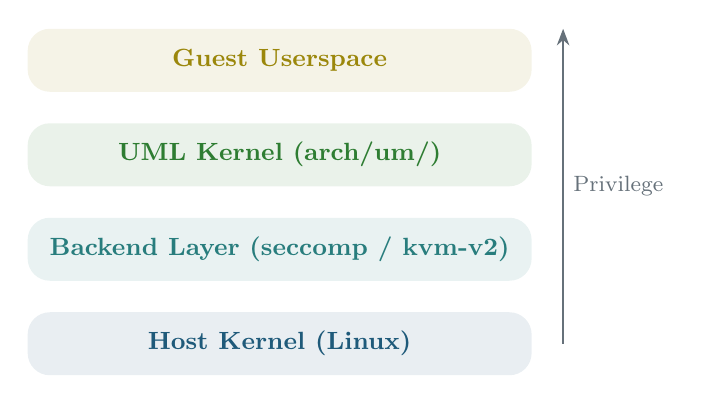
\begin{tikzpicture}[scale=0.8]
  % Stylized layer diagram
  \fill[UMLBlue!10,rounded corners=8pt] (-4,-0.5) rectangle (4,0.5);
  \fill[UMLTeal!10,rounded corners=8pt] (-4,1) rectangle (4,2);
  \fill[UMLGreen!10,rounded corners=8pt] (-4,2.5) rectangle (4,3.5);
  \fill[KernelGold!10,rounded corners=8pt] (-4,4) rectangle (4,5);

  \node[font=\small\bfseries,color=UMLBlue] at (0,0) {Host Kernel (Linux)};
  \node[font=\small\bfseries,color=UMLTeal] at (0,1.5) {Backend Layer (seccomp / kvm-v2)};
  \node[font=\small\bfseries,color=UMLGreen] at (0,3) {UML Kernel (arch/um/)};
  \node[font=\small\bfseries,color=KernelGold] at (0,4.5) {Guest Userspace};

  \draw[-{Stealth[length=6pt]},thick,color=UMLMuted] (4.5,0) -- (4.5,5)
    node[midway,right,font=\footnotesize] {Privilege};
\end{tikzpicture}

\vfill

{\small
Based on the \texttt{mjbommar/linux} kernel tree, branch \texttt{next}\\
7 series-level commits on \texttt{torvalds/master} (v7.1-rc5+)\\[0.5em]
\textit{Prepared with assistance from Claude (Anthropic)}
}
\end{titlepage}

% ===== FRONT MATTER =====
\frontmatter
\tableofcontents
\newpage
\listoffigures
\listoftables

% ===== MAIN MATTER =====
\mainmatter

% ==========================================================================
%  Chapter 1 — Introduction
% ==========================================================================
\chapter{Introduction}
\label{ch:introduction}

\epigraph{%
  The best way to understand a kernel is to run it where you can poke at it.%
}{Jeff Dike, 2000}

\section{What is User-Mode Linux?}
\label{sec:intro-what-is-uml}

User-Mode Linux (\UML{}) is an architecture port of the Linux kernel in which
the kernel itself executes as an ordinary userspace process on a host Linux
system.  Where a conventional kernel runs on bare metal---managing page tables,
servicing interrupts, and scheduling threads with the full authority of CPU ring
0---\UML{} performs all of these functions from ring 3, mediating access to host
resources through the host kernel's system call interface.

In the Linux source tree, \UML{} lives alongside x86, ARM, RISC-V, and the
other architecture ports under \umlpath{arch/um/}.  It shares the same
scheduler, the same VFS layer, the same memory management subsystem, and the
same networking stack as every other port.  The code that differs is precisely
the code that must differ: the low-level trap handling, context switching,
timer management, and memory mapping routines that, on hardware architectures,
speak directly to the CPU and chipset.  In \UML{}, these routines instead call
\syscall{clone}, \syscall{mmap}, \syscall{sigaction}, \syscall{ioctl}, and a
handful of other host system calls.

Jeff Dike created \UML{} in 1999--2000 and presented it at the USENIX Annual
Linux Showcase in Atlanta~\cite{dike2000}.  The original implementation used
the \texttt{ptrace} system call to intercept guest system calls: the \UML{}
kernel ran as a tracing process that caught every \texttt{SIGTRAP} delivered
when a guest userspace process invoked a system call.  This mechanism, while
conceptually elegant, imposed a heavy performance penalty---each guest syscall
required multiple context switches between the tracing kernel and the traced
guest---and the subsequent two decades of \UML{} development can be read as a
sustained effort to reduce that overhead.

The architecture is best understood through the Popek--Goldberg
framework~\cite{popek1974}.  A \emph{virtual machine monitor} (VMM)
must faithfully reproduce the behavior of the underlying machine for guest
software while retaining control over resource allocation.  Traditional VMMs
achieve this by exploiting hardware privilege rings: the guest kernel believes
it runs in ring 0, but the VMM intercepts sensitive instructions from a more
privileged mode.  \UML{} inverts this arrangement.  There is no privilege
separation \emph{at the hardware level} between the \UML{} kernel and its
guests; instead, the host kernel enforces separation through the ordinary
process isolation guarantees of Linux itself.  The \UML{} kernel and its guest
processes are all host-level processes.  What distinguishes them is that the
\UML{} kernel interposes on guest system calls before they can reach the
host---first via \texttt{ptrace}, later via \Seccomp{} filters, and now,
in the v2 redesign, optionally via \KVM{}.

\begin{figure}[ht]
\centering
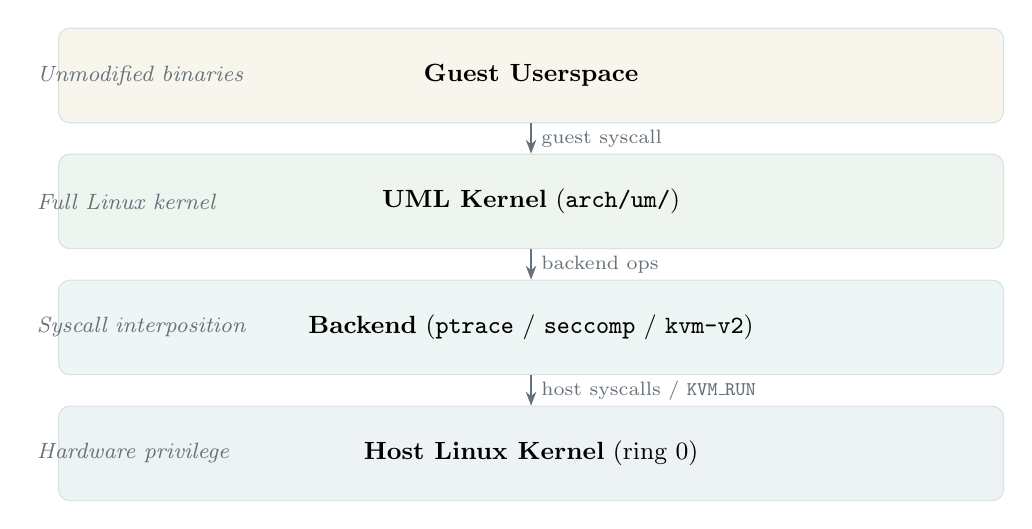
\begin{tikzpicture}[
    layer/.style={
      draw=UMLGrid,
      fill=#1,
      minimum width=12cm,
      minimum height=1.2cm,
      rounded corners=4pt,
      font=\small
    },
    label/.style={
      font=\footnotesize\itshape,
      text=UMLMuted,
      anchor=west
    },
    arrow/.style={
      -{Stealth[length=5pt]},
      thick,
      color=UMLMuted
    }
  ]

  \node[layer=UMLBlue!8]  (host)    at (0,0)   {\textbf{Host Linux Kernel} (ring 0)};
  \node[layer=UMLTeal!8]  (backend) at (0,1.6)  {\textbf{Backend} (\texttt{ptrace} / \Seccomp{} / \KVMvTwo{})};
  \node[layer=UMLGreen!8] (uml)     at (0,3.2)  {\textbf{UML Kernel} (\umlpath{arch/um/})};
  \node[layer=KernelGold!8](guest)  at (0,4.8)  {\textbf{Guest Userspace}};

  \node[label] at (-6.4,0)   {Hardware privilege};
  \node[label] at (-6.4,1.6) {Syscall interposition};
  \node[label] at (-6.4,3.2) {Full Linux kernel};
  \node[label] at (-6.4,4.8) {Unmodified binaries};

  \draw[arrow] (guest.south) -- (uml.north)
    node[midway,right,font=\scriptsize] {guest syscall};
  \draw[arrow] (uml.south) -- (backend.north)
    node[midway,right,font=\scriptsize] {backend ops};
  \draw[arrow] (backend.south) -- (host.north)
    node[midway,right,font=\scriptsize] {host syscalls / \texttt{KVM\_RUN}};

\end{tikzpicture}
\caption[UML architectural layers]{%
  The four-layer \UML{} architecture.  Guest userspace programs issue system
  calls that are trapped by the \UML{} kernel.  The \UML{} kernel services
  these using standard Linux kernel subsystems, performing I/O through the
  backend and host kernel layers.
}
\label{fig:intro-layers}
\end{figure}


\section{Why UML Matters}
\label{sec:intro-why}

In a landscape crowded with virtualization and sandboxing technologies---\KVM{},
Xen~\cite{barham2003}, Firecracker~\cite{firecracker}, gVisor~\cite{gvisor},
containers, unikernels---it is reasonable to ask whether \UML{} still
has a role.  The answer is emphatically yes, precisely because \UML{} occupies
a unique and underserved niche in the design space.

\subsection{The real kernel, not a reimplementation}

gVisor's Sentry~\cite{gvisor} reimplements the Linux system call interface in
Go.  It is an impressive feat of engineering, but it is not the Linux kernel:
subtle semantic differences arise when the Sentry's interpretation of a system
call diverges from the kernel's.  The Linux Kernel Library
(\textsc{LKL})~\cite{lkl} compiles the kernel as a linkable library, but
strips away process scheduling and user/kernel separation.

\UML{}, by contrast, \emph{is} the Linux kernel.  Every syscall handler,
every scheduler decision, every lock acquisition follows the same code paths
as a kernel running on x86 hardware.  A bug found in \UML{} is a bug in
mainline Linux, and a fix validated in \UML{} is a fix for every architecture.
This fidelity is not accidental---it is a consequence of \UML{} being an
\texttt{arch/} port, sharing all architecture-independent code with the rest
of the tree.

\subsection{Full user/kernel separation}

Unlike \textsc{LKL}, which runs kernel code in the same address space and
privilege level as the application, \UML{} maintains genuine user/kernel
separation.  Guest userspace processes run in separate host processes with
restricted memory mappings.  A bug in a guest program cannot corrupt \UML{}
kernel data structures any more than a bug in a userspace program can corrupt
a bare-metal kernel.  This separation is essential for security research,
kernel fuzzing, and any application where the guest is untrusted.

\subsection{No hardware virtualization requirements}

\KVM{}~\cite{kivity2007} and Firecracker~\cite{agache2020} require hardware
virtualization extensions (Intel VT-x or AMD-V) and access to
\umlpath{/dev/kvm}.  In many environments---containerized CI/CD runners,
shared cloud instances, locked-down workstations---\texttt{/dev/kvm} is
unavailable.  \UML{} with the \texttt{ptrace} or \Seccomp{} backends has no
such requirement: it runs wherever a Linux userspace process can run.  This
makes it uniquely suited for environments where hardware-assisted
virtualization is either absent or administratively prohibited.

\subsection{Application domains}
\label{sec:intro-applications}

The combination of kernel fidelity, process isolation, and minimal host
requirements makes \UML{} valuable across a range of application domains:

\begin{description}[style=nextline,leftmargin=2em]
  \item[Kernel development and debugging.]
    A developer can compile the kernel, run it under \texttt{gdb}, set
    breakpoints in the scheduler, single-step through the page fault handler,
    and inspect kernel data structures---all from an ordinary terminal.
    No reboot, no serial console, no JTAG probe.

  \item[Kernel fuzzing.]
    Coverage-guided fuzzers like syzkaller~\cite{syzkaller} and
    kAFL~\cite{schumilo2017} benefit from fast boot times and deterministic
    execution.  \UML{} boots in under a second, can be snapshot/restored
    without hardware support, and when combined with \textsc{LKL}-style
    in-process execution for the fast path, can achieve millions of syscalls
    per second.

  \item[Network simulation.]
    Projects like Netkit~\cite{pizzonia2008} and Marionnet~\cite{marionnet}
    use \UML{} to run dozens or hundreds of virtual Linux machines, each with
    its own networking stack, connected by virtual switches and routers.
    Students and researchers can build and tear down complex network topologies
    entirely in userspace.

  \item[Security research.]
    \UML{} provides a complete kernel attack surface without requiring trust in
    hardware or a hypervisor.  Researchers can study kernel exploits, test
    sandboxing mechanisms, and develop mitigations in a fully controlled
    environment.

  \item[CI/CD and automated testing.]
    Kernel selftests, \texttt{kselftest} suites, and distribution build
    processes benefit from a lightweight kernel environment that can be
    instantiated in seconds inside a container or a GitHub Actions runner.

  \item[Education.]
    \UML{} turns the kernel into something a student can compile, run, modify,
    and observe without risk to the host system---lowering the barrier to
    kernel development from ``dedicated test machine'' to ``laptop terminal.''
\end{description}


\section{The Current Moment}
\label{sec:intro-moment}

This report is written at a moment of unusual convergence for \UML{}.  Five
developments, none individually decisive but collectively transformative,
have created a window of opportunity for the most significant redesign of
\UML{} since its creation.

\paragraph{1. The \Seccomp{} backend reaches mainline.}
The \Seccomp{} backend, which replaces the decades-old \texttt{ptrace}
mechanism with \texttt{SECCOMP\_IOCTL\_NOTIF\_SEND}-based syscall interception,
was merged for Linux 6.16.  This single change reduced guest syscall overhead
from approximately \SI{3}{\micro\second} (ptrace round-trip) to roughly
\SI{300}{\nano\second}, making \UML{} competitive with lightweight hypervisors
for I/O-intensive workloads.

\paragraph{2. SMP support lands.}
Historically, \UML{} was a uniprocessor architecture.  The addition of SMP
support---mapping \UML{} virtual CPUs to host threads with proper inter-processor
interrupt (IPI) emulation and TLB synchronization---allows \UML{} to exercise
the kernel's concurrency paths, which is precisely where the most dangerous
bugs hide.

\paragraph{3. gVisor's systrap validates swappable backends.}
Google's gVisor project demonstrated with its systrap platform~\cite{gvisor-systrap}
that a syscall-interposition system can support multiple backend mechanisms
behind a common interface.  The gVisor Sentry originally used \texttt{ptrace},
then \KVM{}, then systrap---each time improving performance while maintaining
the same guest-facing semantics.  This architectural precedent directly informed
the backend-ops abstraction in the \UML{} v2 redesign.

\paragraph{4. \textsc{LKL} shows what speed is possible.}
The Linux Kernel Library~\cite{lkl,purdila2010} compiles Linux as a
single-threaded library with no MMU or process separation.  It achieves
extraordinary fuzzing throughput---millions of operations per second---at
the cost of fidelity: there is no guest userspace, no scheduling, no realistic
attack surface.  \textsc{LKL} represents one extreme of the speed--fidelity
tradeoff.  The \UML{} v2 redesign aims to approach \textsc{LKL}'s speed while
retaining \UML{}'s complete kernel semantics.

\paragraph{5. The kernel community accepts AI-assisted development.}
The addition of the \texttt{coding-assistants.html} document to the kernel's
\umlpath{Documentation/process/} directory~\cite{coding-assistants} signals an
institutional willingness to engage with AI-assisted patch development.  The v2
redesign demonstrates what becomes possible when AI tools are used not to
generate mechanical patches, but to navigate architectural decisions across a
codebase of \num{30000000}+ lines of code.


\section{Report Structure}
\label{sec:intro-structure}

This report is organized as follows:

\begin{description}[style=nextline,leftmargin=2em,font=\bfseries]
  \item[Chapter~\ref{ch:introduction}: Introduction]
    (This chapter.)  Motivation, context, and scope.

  \item[Chapter 2: History]
    The evolution of \UML{} from Dike's original \texttt{ptrace}-based
    prototype through the TT/SKAS transition, the years of maintenance
    mode, and the recent resurgence of interest.

  \item[Chapter 3: Foundations]
    Background material on virtualization theory (Popek--Goldberg), Linux
    process primitives (\texttt{ptrace}, \Seccomp{}, \texttt{clone},
    \texttt{mmap}), and the \KVM{} API---the building blocks from which
    \UML{} is constructed.

  \item[Chapter 4: UML Architecture]
    The high-level architecture of \UML{}: how it maps kernel abstractions
    (virtual memory, interrupts, timers, I/O) onto host-level mechanisms.
    The backend-ops abstraction layer and its role in enabling pluggable
    backends.

  \item[Chapter 5: UML Implementation]
    A detailed walk through the \UML{} source tree, covering boot
    sequence, system call handling, memory management, signal delivery,
    SMP, and device I/O.

  \item[Chapter 6: The \KVMvTwo{} Backend]
    Design and implementation of the new \KVM{}-based backend.  How
    \texttt{KVM\_CREATE\_VM}, \texttt{KVM\_CREATE\_VCPU}, and
    \texttt{KVM\_RUN} are used to achieve approximately \SI{100}{\nano\second}
    syscall latency for guest-to-kernel transitions.

  \item[Chapter 7: Applications]
    Detailed case studies: kernel debugging under \texttt{gdb}, syzkaller
    integration, network simulation, CI/CD pipelines, and educational use.

  \item[Chapter 8: Related Work]
    Comparison with \KVM{}/QEMU, Xen, Firecracker, gVisor, \textsc{LKL},
    Dune~\cite{belay2012}, containers, and unikernels~\cite{madhavapeddy2013}.

  \item[Chapter 9: The v2 Redesign]
    The complete contribution of this work: backend-ops abstraction, \KVMvTwo{}
    backend, SMP, snapshot/restore, record/replay, comprehensive selftests,
    and the Rust \texttt{umlctl} launcher tool.  Design rationale, trade-offs,
    and lessons learned.

  \item[Chapter 10: Conclusion]
    Summary of contributions, open problems, and future directions.

  \item[Appendix A: Source Map]
    Annotated directory listing of the \UML{} source tree with the v2
    additions.

  \item[Appendix B: Benchmarks]
    Raw benchmark data and methodology for the performance measurements
    cited throughout the report.
\end{description}


\section{Contributions of This Work}
\label{sec:intro-contributions}

The v2 redesign of User-Mode Linux, developed by Michael Bommarito with
AI-assisted tooling, contributes the following:

\begin{enumerate}[leftmargin=2em]
  \item \textbf{Backend operations abstraction.}
    A \texttt{struct um\_backend\_ops} interface
    (defined in \umlpath{arch/um/include/shared/backend.h})
    that decouples the \UML{} kernel from any single syscall-interposition
    mechanism.  The abstraction defines a contract for backend lifecycle
    management, guest process creation, syscall interception, context switching,
    and memory mapping.  New backends can be added by implementing this
    interface without modifying core \UML{} code.

  \item \textbf{The \KVMvTwo{} backend.}
    A new backend that uses the \KVM{} API to run \UML{} guest code in
    hardware-accelerated virtual CPUs.  When the guest executes a system call,
    the resulting VM exit is handled directly by the \UML{} kernel---no
    \texttt{ptrace} round-trip, no \Seccomp{} notification.  Measured syscall
    latency is approximately \SI{100}{\nano\second}, a $3\times$ improvement
    over \Seccomp{} and a $30\times$ improvement over \texttt{ptrace}.

  \item \textbf{SMP support.}
    Multi-processor support for \UML{}, mapping virtual CPUs to host threads
    with proper IPI emulation, TLB shootdown, and memory barrier semantics.
    This enables \UML{} to exercise---and expose bugs in---the kernel's
    concurrent code paths.

  \item \textbf{Snapshot and restore.}
    Mechanisms for capturing and restoring the complete state of a running
    \UML{} instance, enabling fast restart for fuzzing workloads and
    reproducible bug investigation.

  \item \textbf{Record and replay.}
    Deterministic record/replay infrastructure that captures non-deterministic
    events (timer interrupts, I/O completions) during execution and replays
    them faithfully, enabling time-travel debugging of kernel code.

  \item \textbf{Comprehensive selftests.}
    A test suite under \umlpath{tools/testing/selftests/um/} covering backend
    lifecycle, syscall interception, SMP behavior, memory management, and
    performance regression detection.

  \item \textbf{The \texttt{umlctl} launcher.}
    A Rust-based command-line tool for building, configuring, launching, and
    managing \UML{} instances.  It handles kernel compilation, root filesystem
    preparation, backend selection, and instance lifecycle, reducing the barrier
    to entry from a page of shell commands to a single invocation.
\end{enumerate}

\noindent
These contributions are organized as seven series-level commits on
the \texttt{mjbommar/linux} tree (branch \texttt{next}), based on
\texttt{torvalds/master} at v7.1-rc5.  Each series is independently
reviewable and bisectable.

\bigskip

The remainder of this report proceeds from history and theory
(Chapters~2--3), through architecture and implementation (Chapters~4--6),
to applications and evaluation (Chapters~7--8), and concludes with
the complete v2 redesign narrative (Chapter~9) and future
directions (Chapter~10).

% ==========================================================================
%  Chapter 2: History of User-Mode Linux
% ==========================================================================

\chapter{History of User-Mode Linux}
\label{ch:history}

\epigraph{``I'm doing a (free) operating system (just a hobby, won't be big and
professional like gnu) for 386(486) AT clones.''}{---Linus Torvalds, 1991~\cite{torvalds1991}}

\noindent
User-Mode Linux did not emerge in a vacuum.  Its existence is a consequence of
design decisions made years before its conception---most notably, the Linux
kernel's clean separation of architecture-dependent and architecture-independent
code.  This chapter traces the full arc: from the early Linux kernel and the
debugging problems that motivated \UML{}, through its creation and golden era, into
a decade of decline, and finally to the revival that produced the modern
multi-backend architecture described in this report.

% ------------------------------------------------------------------
\section{The Linux Kernel Before UML (1991--1999)}
\label{sec:history-prelude}
% ------------------------------------------------------------------

On October 5, 1991, Linus Torvalds posted the famous announcement to
\texttt{comp.os.minix} describing his ``free minix-like kernel sources for
386-AT''~\cite{torvalds1991}.  Linux 0.01 was a monolithic kernel that ran
exclusively on the Intel 80386 processor.  It supported a single address space
layout, a single disk controller, and a handful of system calls.  But it
compiled, it booted, and it was free.

Over the next eight years, Linux grew at an extraordinary rate.  The 1.0 release
(March 1994) was the first declared stable; 2.0 (June 1996) added symmetric
multiprocessing (SMP) support and multiple architecture ports---Alpha, SPARC,
MIPS, m68k, PowerPC.  The 2.2 release (January 1999) brought improved SMP
scalability, better networking, and the beginnings of enterprise-grade
reliability.  By the end of the decade, Linux was running on everything from
embedded routers to IBM mainframes, and kernel development involved hundreds of
contributors worldwide.

\subsection{The \texttt{arch/} Abstraction}
\label{sec:history-arch-abstraction}

The most architecturally consequential decision of this era was the directory
structure that emerged to support multiple hardware platforms.  Rather than
scattering \texttt{\#ifdef} conditionals throughout the code, Linux adopted a
clean split: the \umlpath{arch/} directory contained all architecture-specific
code---trap handling, context switching, page table manipulation, signal
delivery, system call entry---while the rest of the tree
(\umlpath{kernel/}, \umlpath{mm/}, \umlpath{fs/}, \umlpath{net/},
\umlpath{drivers/}) remained architecture-independent.

Each architecture port implemented a well-defined interface: functions like
\texttt{switch\_to()}, \texttt{copy\_thread()}, \texttt{start\_thread()}, and
page table accessors (\texttt{pgd\_val()}, \texttt{pte\_val()}, etc.).  The
interface was never formally specified---it evolved organically as new
architectures were added---but it was remarkably clean.  A new port meant
implementing perhaps 50--100 key functions and data structures, after which the
entire kernel (scheduler, VFS, networking stack, memory manager) would work
without modification.

This abstraction was conceived to support hardware architectures: x86, Alpha,
SPARC, ARM.  No one anticipated that someone would write an ``architecture'' where
the hardware was another copy of Linux itself.

\subsection{The Debugging Problem}
\label{sec:history-debugging}

Kernel debugging in the 1990s was, to put it charitably, primitive.  The primary
tools were:

\begin{description}[leftmargin=2em,labelindent=1em]
  \item[\texttt{printk()}] The kernel's printf equivalent.  Developers added
    \texttt{printk()} calls, rebuilt the kernel, rebooted, reproduced the bug,
    read the console output.  This cycle could take minutes to hours depending on
    the bug.

  \item[Serial console] A step up: connect two machines with a serial cable, use
    one to observe the other's console output.  Essential for debugging panics
    where the screen was already dead.

  \item[\texttt{kgdb}] An external patch (never merged into mainline during this
    era) that allowed GDB to connect to a running kernel via serial line.  It
    worked, but it required a second machine, serial hardware, and careful setup.
    Breakpoints in interrupt handlers were hazardous.

  \item[\texttt{kdb}] SGI's kernel debugger, also out-of-tree.  More capable
    than \texttt{kgdb} for some workflows, but equally dependent on specialized
    hardware setups.

  \item[Crash analysis] When the kernel panicked, you got a register dump and a
    call trace.  Interpreting these required intimate knowledge of the
    architecture's calling conventions and the ability to cross-reference
    addresses against \texttt{System.map}.
\end{description}

\noindent
What you could \emph{not} do was the thing that every application programmer
took for granted: run the code under a debugger.  You could not set a breakpoint
in the scheduler and single-step through a context switch.  You could not attach
\texttt{valgrind} to the memory manager.  You could not run the kernel under
\texttt{strace} to see what system calls it made.  The kernel was the bottom of
the stack---there was nothing underneath it to provide these services.

This asymmetry between kernel and userspace development productivity was a
constant source of frustration.  It also meant that certain classes of bugs---race
conditions, memory corruption, subtle locking errors---were disproportionately
expensive to diagnose and fix.  The kernel needed a way to be a \emph{process}.

% ------------------------------------------------------------------
\section{Jeff Dike and the Creation of UML (1999--2001)}
\label{sec:history-creation}
% ------------------------------------------------------------------

Jeff Dike was a kernel developer at VA Linux Systems in the late 1990s.  VA
Linux was one of the first companies to build a business around Linux, and its
engineers were deeply involved in kernel development.  Dike had been thinking
about the debugging problem and, more broadly, about how to make the kernel more
accessible for development and experimentation.

His key insight was deceptively simple: \emph{the Linux kernel's
\texttt{arch/} abstraction is clean enough that you can write an
``architecture'' where the ``hardware'' is the host kernel's system call
interface.}

Consider what an architecture port must provide: a way to create and switch
between address spaces, a way to handle interrupts and traps, a way to start and
stop the CPU, a way to manage memory pages.  All of these have direct analogs in
the POSIX API:

\begin{itemize}[nosep]
  \item Address spaces $\to$ \syscall{mmap}, \syscall{mprotect}, \syscall{munmap}
  \item Interrupts $\to$ POSIX signals (SIGALRM for the timer tick, SIGIO for I/O)
  \item Context switching $\to$ \syscall{setjmp}/\syscall{longjmp} or signal stack manipulation
  \item Trap handling $\to$ \syscall{ptrace} to intercept guest system calls
  \item Physical memory $\to$ a large \syscall{mmap}'d file (the ``physical memory'' file)
  \item Block devices $\to$ host files accessed via \syscall{read}/\syscall{write}
  \item Network devices $\to$ host TAP/TUN interfaces or Unix domain sockets
\end{itemize}

\noindent
The resulting system would not be an emulator.  It would not translate
instructions or simulate hardware.  It \emph{would be} the Linux kernel---the
same source code, compiled for a different ``architecture.''  The kernel's
scheduler would schedule processes; its VFS would manage file systems; its TCP/IP
stack would route packets.  The only difference was that instead of running on
bare metal (or in a hypervisor), it ran as a collection of ordinary Linux
processes.

\subsection{The Initial Announcement}
\label{sec:history-announcement}

Dike announced User-Mode Linux on the Linux Kernel Mailing List (LKML) in
1999.  The initial response was a mixture of fascination and skepticism.  Some
developers immediately grasped the implications for debugging and testing.
Others questioned whether the performance overhead would make it practical.
A few doubted whether the \texttt{arch/} interface was really clean enough to
support such an unconventional ``architecture.''

Dike persisted.  By 2000, he had a working implementation that could boot a
full Linux system, run a shell, and execute userspace programs.  He presented
the work at the 4th Annual Linux Showcase and Conference (ALS) in
Atlanta~\cite{dike2000}.

\subsection{The Tracing Thread (TT) Mode}
\label{sec:history-tt}

The first \UML{} execution engine used a model called ``tracing thread'' (tt)
mode.  The architecture was as follows:

\begin{enumerate}[nosep]
  \item The \UML{} kernel ran as a single host process (the ``tracing thread'').
  \item Each guest userspace process was a separate host process.
  \item The tracing thread used \syscall{ptrace} to attach to every guest
    process as a debugger.
  \item When a guest process made a system call, the host kernel delivered a
    \texttt{SIGTRAP} to the tracing thread (via the ptrace notification
    mechanism).
  \item The tracing thread intercepted the system call, extracted its arguments
    from the guest's registers, dispatched it to the \UML{} kernel's system call
    handler, wrote the result back into the guest's registers, and resumed the
    guest.
\end{enumerate}

\noindent
This worked, and it was conceptually elegant: ptrace was designed exactly for
this kind of process inspection and control.  But it had significant drawbacks:

\begin{description}[leftmargin=2em,labelindent=1em]
  \item[Host visibility] Every guest process appeared as a real process on the
    host.  If the guest ran 500 processes, the host's process table showed 500+
    entries.  This was confusing for administrators and made it impossible to
    cleanly distinguish guest and host processes.

  \item[Security] Because guest processes were real host processes, they had
    real PIDs, real signal delivery, and real access to \texttt{/proc/self/}.
    A sufficiently determined attacker inside the guest could potentially
    escape---for example, by exploiting ptrace race conditions or by directly
    invoking host system calls that the tracing thread failed to intercept.

  \item[Performance] Every guest system call required \emph{at minimum} four
    context switches: guest $\to$ host kernel (for the syscall trap) $\to$
    tracing thread (SIGTRAP delivery) $\to$ host kernel (to resume guest) $\to$
    guest.  In practice, the overhead was worse because the tracing thread also
    needed to read and write guest registers via \texttt{PTRACE\_PEEKUSR} and
    \texttt{PTRACE\_POKEUSR}.  Each such operation was itself a system call.

  \item[Signal handling] Delivering a signal to a guest process required
    elaborate coordination between the tracing thread, the host kernel's signal
    machinery, and the guest's signal handling code.  Getting this right was one
    of the most complex parts of the implementation.
\end{description}

\noindent
Despite these limitations, tt mode was a remarkable achievement.  For the first
time, a developer could run the Linux kernel under GDB, set breakpoints in the
scheduler, single-step through context switches, and use \texttt{valgrind} to
detect memory errors.  The productivity impact was immediate and
substantial~\cite{dike2001}.

\subsection{Key Insight: UML Is Not an Emulator}
\label{sec:history-not-emulator}

It is worth emphasizing a point that was frequently misunderstood (and still
is): \UML{} is not an emulator.  Emulators like Bochs or (later) QEMU translate
machine instructions from one ISA to another, or simulate hardware devices.
\UML{} does neither.  The guest kernel code is \emph{compiled natively} for the
host architecture.  When a function like \texttt{schedule()} runs inside \UML{},
it is executing the same compiled x86-64 instructions that it would on bare
metal.  The architecture layer merely provides a different implementation of the
hardware abstraction---one that talks to the host kernel instead of to physical
hardware.

This distinction has profound implications for fidelity.  Code that works in
\UML{} will work on bare metal (modulo hardware-specific drivers), and bugs found
in \UML{} are real kernel bugs.  \UML{} is the kernel, running in a different
environment.

% ------------------------------------------------------------------
\section{The SKAS Evolution (2002--2006)}
\label{sec:history-skas}
% ------------------------------------------------------------------

The limitations of tt mode---particularly the security and host-visibility
problems---motivated a fundamental redesign of the execution engine.  The
result was SKAS: \textbf{S}eparate \textbf{K}ernel \textbf{A}ddress
\textbf{S}pace mode.

\subsection{The Problem with Shared Address Spaces}
\label{sec:history-skas-problem}

In tt mode, the \UML{} kernel code ran in the same address space as the
guest process it was currently serving.  This meant that a guest process
could, in principle, read or corrupt kernel data structures.  The tracing
thread did its best to prevent this, but the fundamental architecture made
strong isolation impossible.

The goal of SKAS was to give the \UML{} kernel its own address space,
separate from all guest processes.  When a guest process made a system call,
execution would switch to the kernel address space, handle the call, and
switch back---just as a real kernel switches between kernel and user mode
via privilege ring transitions.

\subsection{SKAS0: No Host Kernel Patches Required}
\label{sec:history-skas0}

The first SKAS implementation, known as SKAS0, achieved address space
separation using only standard host kernel facilities.  The technique was
ingenious:

\begin{enumerate}[nosep]
  \item The \UML{} kernel ran in a dedicated host process with its own
    address space.
  \item Guest processes each had their own host process (as in tt mode),
    but the tracing thread could now switch the guest process's memory
    mappings to point at the kernel's address space when needed.
  \item Address space switching was accomplished via careful use of
    \texttt{PTRACE\_SYSCALL} to intercept \syscall{mmap} calls and remap
    the process's memory.
\end{enumerate}

\noindent
SKAS0 was a major improvement over tt mode.  Guest processes could no longer
directly access kernel memory, and the security model was substantially
stronger.  The performance cost of the address-space switching was nontrivial,
but the security benefits were considered worth it.

\subsection{SKAS3: The /proc/mm Approach}
\label{sec:history-skas3}

SKAS0's address-space manipulation was clever but slow, requiring multiple
system calls per switch.  Dike proposed a host kernel extension---a
\texttt{/proc/mm} interface---that would allow a tracing process to directly
manipulate another process's address space with a single system call.  This
variant was called SKAS3 (the number referring to the host kernel patch
revision that introduced the necessary support).

With \texttt{/proc/mm}, the tracing thread could:
\begin{itemize}[nosep]
  \item Create a new memory management context via \texttt{/proc/mm}
  \item Map and unmap pages in that context with a single \syscall{ioctl}
  \item Switch a traced process between contexts efficiently
\end{itemize}

\noindent
The performance improvement over SKAS0 was significant---roughly 2x for
system-call-intensive workloads.  However, the approach required running a
patched host kernel, which limited adoption.  Most users preferred the
slightly slower SKAS0 over the burden of maintaining a custom host kernel.

\subsection{SKAS4 and the OLS Talks}
\label{sec:history-skas4}

Dike continued refining the approach.  SKAS4 proposed further optimizations
to the host kernel interface, aiming to minimize the number of context switches
required for guest system call handling.  He presented this work at the Ottawa
Linux Symposium in 2006~\cite{dike-ols2006}, building on his earlier OLS 2003
talk~\cite{dike-ols2003} that had focused on making \UML{} ``ready for the
mainstream.''

The SKAS evolution demonstrated a recurring tension in \UML{}'s history:
achieving good performance often required host kernel modifications, but
requiring host kernel modifications limited adoption.  This tension would
recur with every subsequent execution engine, including the seccomp backend
and the \KVMvTwo{} backend described in this report.

\subsection{The Prentice Hall Book}
\label{sec:history-book}

In 2006, Dike published \emph{User Mode Linux} with Prentice
Hall~\cite{dike2006book}.  The book provided the first comprehensive treatment
of \UML{}'s architecture, covering the tt and SKAS execution models, the memory
system, device drivers, networking, and debugging techniques.  It also included
practical guidance on using \UML{} for development, testing, and virtual
hosting.

The book remains the most detailed single source on \UML{}'s original
architecture, although much of the implementation detail it describes has
since been superseded by the seccomp and \KVMvTwo{} backends.

% ------------------------------------------------------------------
\section{Mainline Merge and the Golden Era (2002--2010)}
\label{sec:history-golden}
% ------------------------------------------------------------------

\UML{} was merged into the Linux 2.5 development tree in 2002 and was
included in the 2.6.0 release (December 2003).  The merge was a significant
event: \UML{} was the first virtualization technology to be included in the
mainline Linux kernel.  Its presence in \umlpath{arch/um/} gave it
legitimacy and ensured that kernel API changes would (in theory) be
propagated to the \UML{} port along with every other architecture.

The years from 2002 to roughly 2010 represented \UML{}'s golden era.  During
this period, it was actively developed, widely used, and considered a key
part of the kernel developer's toolkit.

\subsection{Kernel Development and Debugging}
\label{sec:history-kernel-dev}

The primary use case was exactly what Dike had envisioned: making kernel
development easier.  With \UML{}, a developer could:

\begin{itemize}[nosep]
  \item Boot a full Linux system in seconds, without hardware or a heavy VM
  \item Run the kernel under GDB with full source-level debugging
  \item Use \texttt{valgrind} to detect memory errors in kernel code
  \item Test file system changes without risking data on real disks
  \item Reproduce and debug race conditions in the scheduler
  \item Develop and test networking code with virtual networks
  \item Run kernel unit tests without dedicated hardware
\end{itemize}

\noindent
The fast boot time was particularly valuable.  A \UML{} instance could go from
cold start to a shell prompt in under two seconds on contemporary hardware,
compared to minutes for a full hardware boot.  For the edit-compile-test cycle,
this speed difference was transformative.

\subsection{Netkit and Network Simulation}
\label{sec:history-netkit}

One of \UML{}'s most successful applications was Netkit, a network emulation
tool developed by Maurizio Pizzonia and Massimo Rimondini at Roma Tre
University~\cite{pizzonia2008}.  Netkit used \UML{} instances as virtual network
nodes, connected by virtual Ethernet links implemented via Unix domain sockets.

Netkit enabled educators and researchers to create complex network topologies on
a single machine.  A student could configure a multi-router network with BGP,
OSPF, DNS, and DHCP---all running real Linux networking code---on a laptop.
Netkit was widely adopted in networking courses at universities across Europe
and became one of \UML{}'s most visible applications.

The related project Marionnet~\cite{marionnet} provided a graphical interface
for constructing virtual network topologies, further lowering the barrier to
entry for network education and experimentation.

\subsection{Security Research and Honeypots}
\label{sec:history-honeypots}

\UML{} found a natural audience in the security research community.  Its
lightweight isolation made it useful for:

\begin{description}[leftmargin=2em,labelindent=1em]
  \item[Honeypots] Running deliberately vulnerable systems to attract and study
    attackers.  \UML{}'s low overhead made it practical to run many instances
    on a single host, and its isolation (especially in SKAS mode) provided
    reasonable confidence that a compromised guest could not easily escape to
    the host.

  \item[Malware analysis] Executing suspicious binaries in a controlled
    environment where every system call could be observed.

  \item[Intrusion detection research] Running experimental IDS systems against
    realistic kernel and network stacks.
\end{description}

\subsection{Virtual Hosting}
\label{sec:history-vhosting}

Before containers and lightweight VMs became mainstream, \UML{} was used by
some hosting providers to offer virtual private servers (VPS).  Each customer
received a \UML{} instance with its own root filesystem, network configuration,
and process space.  The overhead was lower than full hardware emulation (which
at the time meant something like VMware or Bochs), and the isolation model was
stronger than chroot-based approaches.

Companies like Linode (in its early days, before switching to Xen) and various
European hosting providers offered \UML{}-based VPS products.  While the
performance overhead of ptrace-based system call interception made \UML{} slower
than native execution, it was adequate for many web hosting and
light-computation workloads.

% ------------------------------------------------------------------
\section{Decline and Maintenance Mode (2010--2020)}
\label{sec:history-decline}
% ------------------------------------------------------------------

\UML{}'s decline was not the result of any single event.  It was the
cumulative effect of multiple technological shifts that eroded its competitive
advantages while \UML{} itself stagnated.

\subsection{Hardware Virtualization Changes the Landscape}
\label{sec:history-hwvirt}

The most consequential shift was the arrival of hardware virtualization
support in commodity x86 processors.  Intel released VT-x (originally
codenamed ``Vanderpool'') in late 2005 on the Pentium 4 662 and
672~\cite{intel-vt}.  AMD followed in 2006 with AMD-V (SVM, originally
``Pacifica'')~\cite{amd-svm}.  These extensions added a new privilege
level---VMX root and non-root modes (Intel) or host and guest modes
(AMD)---that allowed a hypervisor to run unmodified guest operating systems
with near-native performance.

The impact on the virtualization landscape was seismic.  Before VT-x/AMD-V,
running an unmodified guest OS on x86 required either full emulation
(slow), binary translation (complex, patented by VMware), or
paravirtualization (required guest OS modifications, as with Xen).
Hardware virtualization made it possible to run unmodified guests with
overhead measured in single-digit percentages rather than factors of 2--10x.

For \UML{}, this was an existential threat.  \UML{}'s ptrace-based system
call interception imposed an overhead of roughly 1--5\,\textmu{}s per guest
system call.  For a workload making 100,000 system calls per second, this
translated to 0.1--0.5 seconds of overhead per second of execution---a
10--50\% performance penalty on a system-call-intensive workload.  Hardware
virtualization reduced the equivalent overhead to tens of nanoseconds per
VM exit, roughly two orders of magnitude faster.

\subsection{KVM: Virtualization in the Kernel}
\label{sec:history-kvm}

The decisive blow came in February 2007, when Avi Kivity's KVM (Kernel-based
Virtual Machine) was merged into Linux 2.6.20~\cite{kivity2007}.  \KVM{}
leveraged VT-x/AMD-V to turn the Linux kernel itself into a hypervisor.  It
was elegant, minimal (the initial patch was under 10,000 lines), and
\emph{fast}.

\KVM{}'s architecture was the mirror image of \UML{}'s.  Where \UML{} ran a
kernel as a userspace process, \KVM{} ran guest kernels in hardware-supported
VM mode, with the host kernel as the hypervisor.  Where \UML{} used ptrace
to intercept system calls, \KVM{} used VT-x/AMD-V to trap only privileged
operations.  Where \UML{} shared the host's physical memory via \syscall{mmap},
\KVM{} used hardware page tables (EPT/NPT) to provide isolated guest physical
address spaces.

Combined with QEMU~\cite{bellard2005} for device emulation, \KVM{} quickly
became the default virtualization solution for Linux.  It offered near-native
performance for CPU-bound workloads and excellent I/O performance via virtio
paravirtualized drivers.  For the use cases where \UML{} had been the best
available option---kernel development, testing, lightweight VMs---\KVM{}/QEMU
was now competitive and often superior.

\subsection{Containers Capture the Lightweight Market}
\label{sec:history-containers}

The other major technological shift was the rise of OS-level virtualization
(containers).  The Linux kernel's cgroup and namespace infrastructure matured
between 2006 and 2013~\cite{soltesz2007,namespaces}, providing the building
blocks for lightweight isolation: PID namespaces (2008), network namespaces
(2009), user namespaces (2012), and cgroup v1 for resource accounting and
limits.

Docker, released in 2013, packaged these primitives into an accessible
developer tool and ignited the container revolution.  For the use case of
``run an isolated Linux environment with low overhead,'' containers offered
effectively zero additional syscall overhead (the guest ran natively, sharing
the host kernel) and millisecond startup times.

Containers did not provide the kernel-level isolation that \UML{} offered---a
container shared the host kernel, so kernel bugs affected all containers---but
for the vast majority of development and deployment workloads, the trade-off
was acceptable.  The combination of near-zero overhead and excellent tooling
made containers the dominant lightweight isolation mechanism.

\subsection{Code Rot and Declining Maintenance}
\label{sec:history-rot}

As users migrated to \KVM{} and containers, developer attention followed.
\UML{}'s maintenance situation deteriorated:

\begin{itemize}[nosep]
  \item The tt mode was eventually removed, simplifying the codebase but
    also removing a working (if slow) execution engine.
  \item SMP support was never completed; \UML{} remained UP-only for over
    a decade.
  \item Various kernel API changes were not properly propagated to
    \umlpath{arch/um/}, causing build breakages that sometimes persisted
    for entire release cycles.
  \item The SKAS0 mode accumulated technical debt, with workarounds and
    hacks layered on top of the original ptrace-based design.
  \item Test coverage was minimal---there were no automated selftests, and
    manual testing was sporadic at best.
  \item Documentation drifted out of date with the actual implementation.
\end{itemize}

\noindent
Richard Weinberger took over as nominal maintainer, and his efforts kept
\UML{} from being removed entirely.  But the subsystem was in maintenance
mode: patches were mostly limited to fixing build breakages caused by core
kernel API changes, with little new feature development.

The perception within the kernel community reflected this state.  \UML{} was
widely viewed as a legacy subsystem---useful in its time, but superseded by
better alternatives.  Proposals to remove it from the tree surfaced
periodically, though they never gained enough traction to reach consensus.

% ------------------------------------------------------------------
\section{The Linux Virtualization Timeline}
\label{sec:history-virt-timeline}
% ------------------------------------------------------------------

To understand \UML{}'s trajectory, it helps to place it in the broader context
of Linux virtualization history.  The following milestones shaped the landscape
in which \UML{} operated:

\subsection{Xen and Paravirtualization (2003)}
\label{sec:history-xen}

Xen, developed at the University of Cambridge, introduced efficient
paravirtualization for x86~\cite{barham2003}.  By modifying the guest OS to
make ``hypercalls'' instead of privileged instructions, Xen achieved
virtualization overhead as low as 2--5\% for many workloads.  Xen was widely
adopted in cloud computing (notably by Amazon Web Services in its early
infrastructure) and demonstrated that high-performance virtualization was
possible even without hardware support.

Xen's success illustrated a design philosophy opposite to \UML{}'s: rather
than making the kernel run as a userspace process, Xen made the hardware (or
a thin software layer mimicking hardware) available to multiple kernel
instances.  Both approaches achieved isolation, but Xen's approach was more
natural for production deployment.

\subsection{Intel VT-x and AMD-V (2005--2006)}
\label{sec:history-hwext}

Intel's VT-x~\cite{intel-vt} and AMD's SVM~\cite{amd-svm} extensions added
hardware support for virtualization to commodity x86 processors.  The key
features included:

\begin{itemize}[nosep]
  \item A new CPU mode (VMX non-root / guest mode) for running guest code
  \item Automatic trapping of privileged operations to the hypervisor
    (VM exits)
  \item Hardware-managed guest/host state save/restore (VMCS/VMCB)
  \item Extended Page Tables (EPT, Intel, 2008) and Nested Page Tables
    (NPT, AMD, 2007) for efficient guest address translation
\end{itemize}

\noindent
These extensions eliminated the need for binary translation or
paravirtualization, enabling hypervisors to run unmodified guest operating
systems with near-native performance.  They also provided a hardware-enforced
security boundary between guest and host that was far stronger than any
software-based approach, including \UML{}'s ptrace-based isolation.

\subsection{KVM Enters Mainline (2007)}
\label{sec:history-kvm-merge}

\KVM{}'s merge into Linux 2.6.20~\cite{kivity2007} was a watershed moment.
It established that the Linux kernel itself would be the primary hypervisor
for Linux-based virtualization, rather than an external project like Xen or
a proprietary product like VMware.  \KVM{}'s tight integration with the Linux
kernel meant that it benefited automatically from every kernel improvement:
scheduler optimizations improved guest scheduling, memory management
improvements improved guest memory performance, and so on.

\subsection{Cgroups and Namespaces Mature (2008--2013)}
\label{sec:history-cgroups}

The cgroup and namespace infrastructure that would eventually underpin
containers was developed incrementally between 2006 and 2013~\cite{namespaces}.
Key milestones included:

\begin{itemize}[nosep]
  \item 2006: cgroup v1 infrastructure merged
  \item 2008: PID namespaces
  \item 2009: Network namespaces
  \item 2012: User namespaces (allowing unprivileged container creation)
  \item 2013: Docker 0.1 released, combining cgroups, namespaces, and
    union filesystems into an accessible tool
\end{itemize}

\noindent
Containers~\cite{soltesz2007} did not provide the same isolation guarantees
as virtual machines (a kernel exploit in a container compromises the host),
but they offered effectively zero overhead and subsecond startup.  For
development workflows and many production deployments, this trade-off was
overwhelmingly attractive.

\subsection{gVisor: A Different Approach (2018)}
\label{sec:history-gvisor}

Google's gVisor~\cite{gvisor}, released in 2018, represented a fascinating
convergence with some of \UML{}'s original ideas.  gVisor implements a
user-space kernel (called Sentry) that intercepts guest system calls and
reimplements them in Go.  Like \UML{}, gVisor runs guest applications as
processes on the host.  Unlike \UML{}, gVisor does not use the Linux kernel
source code---it is a clean-room reimplementation of the Linux system call
interface.

gVisor's original platform used ptrace for system call interception (just
as \UML{}'s tt mode did), and later moved to a KVM-based platform for
better performance.  In 2023, gVisor introduced Systrap, a SIGSYS-based
platform that uses seccomp-bpf for system call interception---conceptually
identical to the approach that Benjamin Berg would bring to \UML{}.

The parallel evolution is striking: two projects, decades apart, converging
on the same insight that seccomp-bpf provides a faster mechanism for system
call interception than ptrace.

\subsection{Firecracker: MicroVMs for Serverless (2020)}
\label{sec:history-firecracker}

Amazon Web Services released Firecracker in 2020~\cite{agache2020}, a
purpose-built virtual machine monitor (VMM) for serverless computing.
Firecracker uses \KVM{} as its hypervisor but strips away nearly all of
QEMU's device emulation complexity, providing only a minimal set of
paravirtualized devices (virtio-net, virtio-block, a serial console).  The
result is a VMM that can boot a guest in approximately 125\,ms and
consumes less than 5\,MB of memory per VM.

Firecracker's existence demonstrated that the performance gap between VMs
and containers could be narrowed dramatically with careful engineering.  It
also showed that for production workloads requiring strong isolation, the
kernel community had converged on \KVM{} as the foundation.

% ------------------------------------------------------------------
\section{The Revival (2020--2026)}
\label{sec:history-revival}
% ------------------------------------------------------------------

Against this backdrop, several independent threads of development converged
in the early 2020s to revive \UML{}.  The motivations were varied, but they
shared a common recognition that \UML{}'s unique position---a real kernel
running as a userspace process---provided capabilities that no other
virtualization technology could match.

\subsection{Benjamin Berg and the Seccomp Backend}
\label{sec:history-seccomp}

The most consequential development was Benjamin Berg's work on a seccomp-based
execution backend.  The idea, building on the seccomp-bpf
framework~\cite{seccomp-bpf} that Will Drewry had added to the kernel in 2012,
was to replace ptrace-based system call interception with SIGSYS-based
notification.

The mechanism works as follows:
\begin{enumerate}[nosep]
  \item A seccomp-bpf filter is installed that matches all system calls from
    guest processes.
  \item When a guest process makes a system call, the kernel generates a
    \texttt{SIGSYS} signal instead of executing the system call.
  \item The signal handler (running in the \UML{} kernel context) examines
    the system call, dispatches it to the appropriate \UML{} kernel handler,
    and manipulates the guest's register state to reflect the result.
  \item Execution resumes in the guest process with the system call appearing
    to have completed normally.
\end{enumerate}

\noindent
The performance advantage over ptrace was substantial.  Ptrace-based
interception required a minimum of two context switches per system call
(guest $\to$ tracer $\to$ guest) plus additional system calls for register
access.  The seccomp approach handled everything within a single signal
delivery, which the kernel could process largely in-place.  Benchmarks showed
roughly 3--4x improvement in system call throughput.

Berg also redesigned the \UML{} process model around futex-based
synchronization, replacing the signal-heavy IPC that the old ptrace backend
had used.  The result was a cleaner, faster, and more maintainable execution
engine.

The seccomp backend was merged into Linux 6.16 (released 2025), marking the
first major new feature to land in \umlpath{arch/um/} in over a decade.

\subsection{Tiwei Bie and SMP Support}
\label{sec:history-smp}

Tiwei Bie (Intel) developed a series of patches to bring SMP support to
\UML{}.  The v4 series implemented multi-CPU scheduling using host threads
as virtual CPUs, with appropriate locking and synchronization to ensure
correct concurrent execution.

SMP support was a long-standing gap in \UML{}'s capabilities.  Modern
kernel code is thoroughly concurrent, with per-CPU data, RCU, and lock-free
algorithms that behave differently on UP and SMP systems.  Running \UML{}
in UP mode meant that an entire class of concurrency bugs---the class that
is most difficult to diagnose and fix---was invisible.

\subsection{Anton Ivanov and Virtio-UML}
\label{sec:history-virtio}

Anton Ivanov contributed virtio-uml, a transport layer that allows \UML{}
to use virtio devices via vhost-user or direct kernel virtio backends.
This work was significant because it connected \UML{} to the broader virtio
ecosystem: instead of implementing custom device models for each device
type (block, network, console), \UML{} could use the same paravirtualized
device stack that \KVM{}/QEMU, Firecracker, and other VMMs used.

\subsection{Hajime Tazaki and the LKL-into-UML RFC}
\label{sec:history-lkl}

Hajime Tazaki submitted an RFC series (reaching v8) proposing to unify the
Linux Kernel Library (LKL)~\cite{lkl,tazaki2019} into \UML{}.  LKL
compiled the Linux kernel as a library that could be linked into userspace
applications, providing access to the kernel's networking stack, file
systems, and other subsystems without running a full VM.

The LKL-into-\UML{} RFC stalled due to the complexity of reconciling LKL's
library model with \UML{}'s process model, but it demonstrated continuing
interest in the fundamental idea of running kernel code in userspace.  It
also highlighted the need for a cleaner backend abstraction---a need that
the modern \texttt{backend\_ops} architecture addresses.

\subsection{The Coding Assistants Policy}
\label{sec:history-ai}

In April 2026, the Linux kernel documentation was updated with
\texttt{coding-assistants.rst}~\cite{coding-assistants}, establishing
official guidelines for AI-assisted kernel development.  While not specific
to \UML{}, this policy change facilitated the rapid development of
infrastructure code (selftests, documentation, build tooling) that had been
a persistent bottleneck.

\subsection{The v2 Architecture}
\label{sec:history-v2}

The convergence of these efforts---seccomp backend, SMP, virtio, and renewed
community interest---created the conditions for a more fundamental redesign.
The v2 architecture, detailed in Chapter~\ref{ch:v2redesign} of this report,
introduces a \texttt{backend\_ops} abstraction layer that cleanly separates
the \UML{} kernel from its execution engine.  This allows multiple backends
(seccomp, \KVMvTwo{}, and potentially others) to coexist, selected at boot
time, while sharing the rest of the kernel infrastructure.

The \KVMvTwo{} backend, described in Chapter~\ref{ch:kvm}, leverages
the same \KVM{} hardware virtualization that powers production cloud
infrastructure, but uses it to accelerate \UML{} rather than to replace it.
This closes the performance gap with bare-metal execution while preserving
\UML{}'s defining advantage: the kernel runs as a debuggable, instrumentable
userspace process.

% ------------------------------------------------------------------
\section{Timeline}
\label{sec:history-timeline-fig}
% ------------------------------------------------------------------

Figure~\ref{fig:timeline} presents a visual timeline of the major events
described in this chapter, placing \UML{}'s development in the context of
the broader Linux virtualization ecosystem.

\begin{figure}[htbp]
\centering
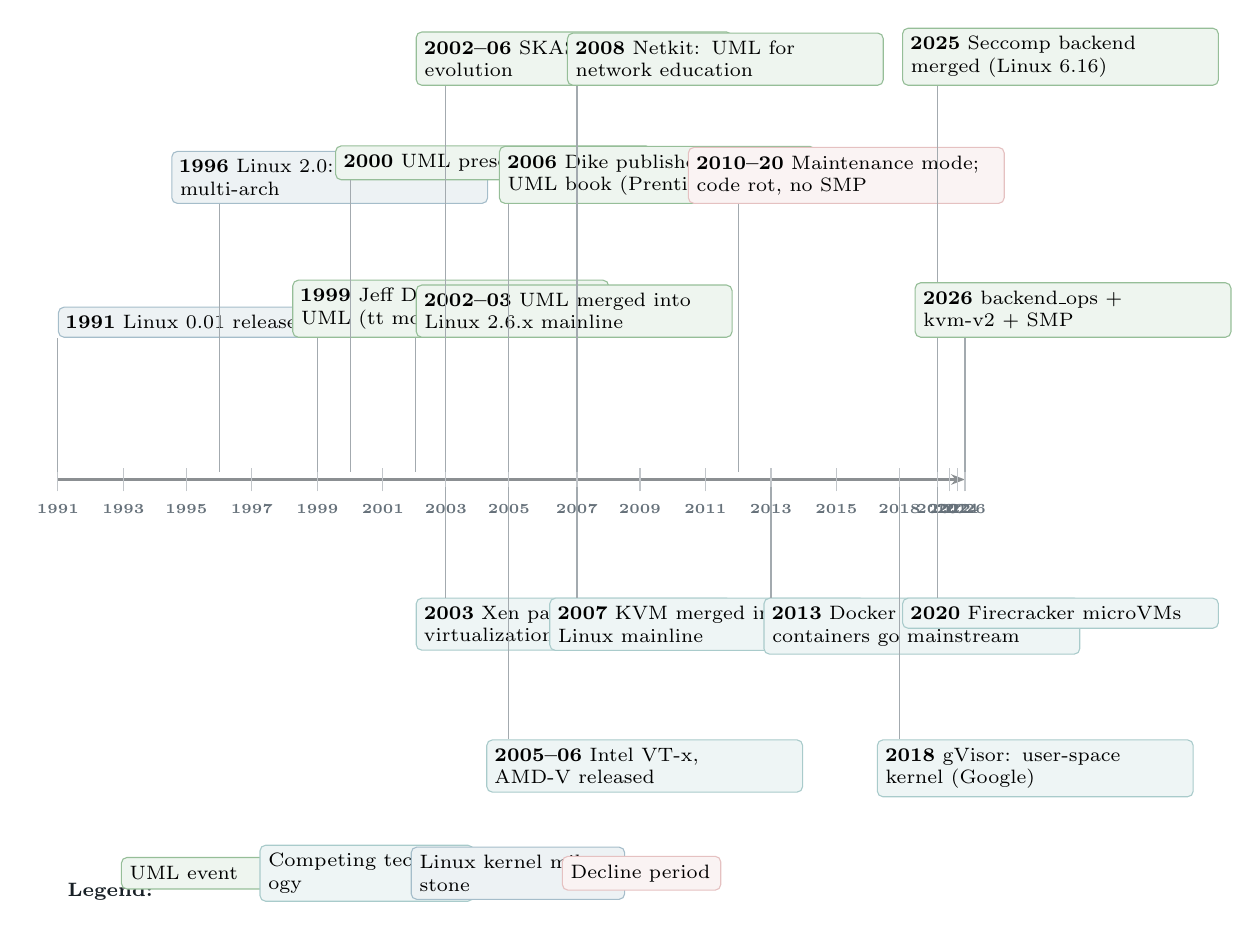
\begin{tikzpicture}[
  x=0.32cm,
  event/.style={fill=UMLBlue!8, draw=UMLBlue!40, rounded corners=2pt,
                font=\scriptsize, text width=3.8cm, align=left, inner sep=3pt},
  virt/.style={fill=UMLTeal!8, draw=UMLTeal!40, rounded corners=2pt,
               font=\scriptsize, text width=3.8cm, align=left, inner sep=3pt},
  uml/.style={fill=UMLGreen!8, draw=UMLGreen!50, rounded corners=2pt,
              font=\scriptsize, text width=3.8cm, align=left, inner sep=3pt},
  decline/.style={fill=UMLRed!6, draw=UMLRed!30, rounded corners=2pt,
                  font=\scriptsize, text width=3.8cm, align=left, inner sep=3pt},
  yearmark/.style={font=\tiny\bfseries, color=UMLMuted},
  connector/.style={thin, color=UMLMuted!60},
]

% --- Axis ---
\draw[thick, color=UMLInk!50, -{Stealth[length=5pt]}] (0,0) -- (36,0);

% Year marks
\foreach \y/\label in {%
  0/1991, 2.6/1993, 5.1/1995, 7.7/1997, 10.3/1999,
  12.9/2001, 15.4/2003, 17.9/2005, 20.6/2007, 23.1/2009,
  25.7/2011, 28.3/2013, 30.9/2015, 33.4/2018, 34.9/2020,
  35.4/2022, 35.7/2024, 36/2026} {
  \draw[color=UMLMuted!40] (\y, -0.15) -- (\y, 0.15);
  \node[yearmark, below] at (\y, -0.2) {\label};
}

% --- Upper events (UML and kernel) ---

% Linux 0.01
\node[event, anchor=south west] (linux) at (0, 1.8)
  {\textbf{1991} Linux 0.01 released};
\draw[connector] (0, 0.1) -- (0, 1.8);

% Linux 2.0 SMP
\node[event, anchor=south west] (smp) at (4.5, 3.5)
  {\textbf{1996} Linux 2.0: SMP,\\multi-arch};
\draw[connector] (6.4, 0.1) -- (6.4, 3.5);

% UML announced
\node[uml, anchor=south west] (uml-ann) at (9.3, 1.8)
  {\textbf{1999} Jeff Dike announces UML (tt mode)};
\draw[connector] (10.3, 0.1) -- (10.3, 1.8);

% UML ALS 2000
\node[uml, anchor=south west] (als) at (11, 3.8)
  {\textbf{2000} UML presented at ALS};
\draw[connector] (11.6, 0.1) -- (11.6, 3.8);

% UML mainline
\node[uml, anchor=south west] (mainline) at (14.2, 1.8)
  {\textbf{2002--03} UML merged into\\Linux 2.6.x mainline};
\draw[connector] (14.2, 0.1) -- (14.2, 1.8);

% SKAS
\node[uml, anchor=south west] (skas) at (14.2, 5.0)
  {\textbf{2002--06} SKAS0/3/4\\evolution};
\draw[connector] (15.4, 0.1) -- (15.4, 5.0);

% Dike book
\node[uml, anchor=south west] (book) at (17.5, 3.5)
  {\textbf{2006} Dike publishes\\UML book (Prentice Hall)};
\draw[connector] (17.9, 0.1) -- (17.9, 3.5);

% Netkit
\node[uml, anchor=south west] (netkit) at (20.2, 5.0)
  {\textbf{2008} Netkit: UML for\\network education};
\draw[connector] (20.6, 0.1) -- (20.6, 5.0);

% UML decline
\node[decline, anchor=south west] (rot) at (25, 3.5)
  {\textbf{2010--20} Maintenance mode;\\code rot, no SMP};
\draw[connector] (27, 0.1) -- (27, 3.5);

% Seccomp backend
\node[uml, anchor=south west] (seccomp) at (33.5, 5.0)
  {\textbf{2025} Seccomp backend\\merged (Linux 6.16)};
\draw[connector] (34.9, 0.1) -- (34.9, 5.0);

% v2 redesign
\node[uml, anchor=south west] (v2) at (34, 1.8)
  {\textbf{2026} backend\_ops +\\kvm-v2 + SMP};
\draw[connector] (36, 0.1) -- (36, 1.8);

% --- Lower events (competing technologies) ---

% Xen
\node[virt, anchor=north west] (xen) at (14.2, -1.5)
  {\textbf{2003} Xen para-\\virtualization};
\draw[connector] (15.4, -0.1) -- (15.4, -1.5);

% VT-x
\node[virt, anchor=north west] (vtx) at (17, -3.3)
  {\textbf{2005--06} Intel VT-x,\\AMD-V released};
\draw[connector] (17.9, -0.1) -- (17.9, -3.3);

% KVM
\node[virt, anchor=north west] (kvm) at (19.5, -1.5)
  {\textbf{2007} KVM merged into\\Linux mainline};
\draw[connector] (20.6, -0.1) -- (20.6, -1.5);

% Docker
\node[virt, anchor=north west] (docker) at (28, -1.5)
  {\textbf{2013} Docker released;\\containers go mainstream};
\draw[connector] (28.3, -0.1) -- (28.3, -1.5);

% gVisor
\node[virt, anchor=north west] (gvisor-node) at (32.5, -3.3)
  {\textbf{2018} gVisor: user-space\\kernel (Google)};
\draw[connector] (33.4, -0.1) -- (33.4, -3.3);

% Firecracker
\node[virt, anchor=north west] (fc) at (33.5, -1.5)
  {\textbf{2020} Firecracker microVMs};
\draw[connector] (34.9, -0.1) -- (34.9, -1.5);

% --- Legend ---
\node[anchor=north west, font=\scriptsize\bfseries, color=UMLInk] at (0, -5.0) {Legend:};
\node[uml, anchor=west, minimum height=0.4cm, text width=1.8cm] at (2.5, -5.0) {UML event};
\node[virt, anchor=west, minimum height=0.4cm, text width=2.5cm] at (8, -5.0) {Competing technology};
\node[event, anchor=west, minimum height=0.4cm, text width=2.5cm] at (14, -5.0) {Linux kernel milestone};
\node[decline, anchor=west, minimum height=0.4cm, text width=1.8cm] at (20, -5.0) {Decline period};

\end{tikzpicture}

\caption{Timeline of User-Mode Linux development in the context of Linux
  kernel and virtualization history (1991--2026).  Upper events relate to
  \UML{} and the Linux kernel; lower events show competing virtualization
  technologies that shaped \UML{}'s trajectory.}
\label{fig:timeline}
\end{figure}

% ------------------------------------------------------------------
\section{Lessons from History}
\label{sec:history-lessons}
% ------------------------------------------------------------------

The arc of \UML{}'s history offers several lessons relevant to the v2
redesign:

\paragraph{Architecture matters more than performance.}
\UML{}'s original \texttt{arch/} insight---that a well-abstracted interface
can be reimplemented on top of very different substrates---was correct in
1999, correct in 2007 when applied to \KVM{}, and remains correct today.
The v2 \texttt{backend\_ops} abstraction applies the same principle within
\UML{} itself: abstracting the execution engine so that new backends (seccomp,
\KVM{}, and future possibilities) can be added without rewriting the rest of
the architecture.

\paragraph{The ptrace tax was real.}
\UML{}'s decade-long decline was not due to a fundamental flaw in the concept
of running a kernel as a userspace process.  It was due to a specific
implementation bottleneck: ptrace-based system call interception was too slow.
The seccomp backend demonstrates that with a better interception mechanism,
the concept remains viable.  The \KVMvTwo{} backend goes further, eliminating
the interception overhead entirely for most operations.

\paragraph{Isolation without hardware is still valuable.}
Containers have no kernel-level isolation.  Hardware VMs provide strong
isolation but require VT-x/AMD-V and cannot be run inside many restricted
environments (CI/CD containers, nested VMs, some cloud instances).  \UML{}
occupies a unique middle ground: real kernel isolation, implemented purely in
software, runnable anywhere a Linux process can run.  This niche has expanded
rather than contracted as CI/CD pipelines and restricted environments have
become ubiquitous.

\paragraph{Debugging the kernel will always matter.}
No amount of hardware virtualization performance eliminates the need to debug
the kernel.  \KVM{}/QEMU provides a debuggable target via GDB's remote
protocol, but the developer experience is qualitatively different from running
the kernel as a native process.  \UML{} allows kernel code to be debugged with
the same tools, workflows, and muscle memory that developers use for userspace
applications.  This advantage is permanent.

\paragraph{Maintenance requires a constituency.}
\UML{}'s decade of rot was a maintenance problem, not a technical one.  The
technology had no organized user community demanding features, no companies
depending on it for production workloads, and no continuous integration
preventing regressions.  The v2 effort addresses this by integrating kselftests,
providing comprehensive documentation, and connecting \UML{} to use cases
(kernel fuzzing, CI/CD, AI-assisted development) that create ongoing
demand for maintenance.

\bigskip
\noindent
With this historical context established, we turn in the next chapter to the
technical foundations on which \UML{} is built: the Linux process model,
the ptrace and seccomp interfaces, and the \KVM{} API.

% ==========================================================================
%  Chapter 3 — Technical Foundations
%  User-Mode Linux: A Comprehensive Technical Report
% ==========================================================================

\chapter{Technical Foundations}
\label{ch:foundations}

\epigraph{Any sufficiently complex virtual machine architecture is
indistinguishable from a real one.}{---with apologies to Arthur C. Clarke}

This chapter establishes the technical concepts required to understand
how a kernel can run as an ordinary userspace process.  We begin with
the classical virtualization taxonomy and show where user-mode kernels
fit---and where they do not.  We then trace the x86 privilege model
from its original ring-based design through the hardware virtualization
extensions that now underpin \KVM{}.  Finally, we examine the Linux
process-model primitives that \UML{} exploits---\syscall{ptrace},
\Seccomp{}, \syscall{mmap}, and the \KVM{} ioctl interface---and compare
the three trap mechanisms that have defined \UML{}'s performance
envelope over the past quarter century.


% ------------------------------------------------------------------
\section{Virtualization Taxonomy}
\label{sec:foundations:taxonomy}

\subsection{The Popek--Goldberg Requirements}

The formal study of virtual machines begins with Goldberg's 1973
taxonomy of \emph{virtual machine monitors} (VMMs)~\cite{goldberg1973}
and the celebrated Popek--Goldberg theorem of 1974~\cite{popek1974}.
Their framework identifies three properties a VMM must satisfy:

\begin{enumerate}[label=\textbf{P\arabic*.},leftmargin=2.5em]
  \item \textbf{Equivalence (Fidelity).}
        A program running under the VMM exhibits behavior identical to
        that observed when running directly on the hardware, with at
        most timing differences.
  \item \textbf{Resource Control (Safety).}
        The VMM retains complete control of the virtualized resources.
        No guest operation may access a resource not explicitly
        allocated to that guest.
  \item \textbf{Efficiency (Performance).}
        A statistically dominant fraction of guest instructions execute
        directly on the hardware without VMM intervention.
\end{enumerate}

The theorem proves that a VMM satisfying all three properties can be
constructed for any \emph{third-generation architecture}\footnote{
  Popek and Goldberg use ``third generation'' to mean a conventional
  von~Neumann machine with a supervisor/user mode split, exemplified by
  IBM~System/370.}
if and only if the set of \emph{sensitive instructions}\footnote{
  Instructions whose behavior depends on the current privilege level or
  that affect the machine's resource-allocation state.}
is a subset of the set of \emph{privileged instructions} (those that
trap when executed in user mode).  When every sensitive instruction is
privileged, the VMM can intercept all guest attempts to observe or
modify machine state by running the guest at a lower privilege level
and catching the resulting traps.

\subsection{Taxonomy of Hypervisors}

Smith and Nair~\cite{smith2005book} refine the taxonomy into two
orthogonal dimensions:

\begin{description}[style=nextline]
  \item[Type~1 (bare-metal) vs.\ Type~2 (hosted) hypervisors.]
    A Type~1 hypervisor runs directly on the hardware with no
    intervening operating system (e.g., VMware ESXi, Xen).  A Type~2
    hypervisor runs as a process atop a host OS (e.g., VMware
    Workstation, VirtualBox).  \KVM{} blurs the boundary: it is a
    loadable module that turns the Linux kernel itself into a Type~1
    hypervisor while simultaneously serving as a host OS.

  \item[Full virtualization vs.\ paravirtualization vs.\ OS-level.]
    Full virtualization presents an unmodified hardware interface to
    the guest; the guest kernel need not know it is virtualized.
    Paravirtualization (exemplified by Xen~\cite{barham2003}) modifies
    the guest kernel to replace sensitive instructions with explicit
    \emph{hypercalls}.  OS-level virtualization (containers) shares a
    single kernel instance and isolates guests via namespaces and
    cgroups~\cite{soltesz2007}.
\end{description}

\subsection{Where User-Mode Kernels Fit}

\UML{} does not fit cleanly into any of these categories, and this
taxonomic awkwardness is part of what makes it interesting.

\begin{itemize}
  \item It is not a hypervisor in the Popek--Goldberg sense, because
        it does not satisfy the Efficiency property: in the original
        \syscall{ptrace}-based design, \emph{every} guest system call
        requires VMM intervention.
  \item It is not OS-level virtualization, because it runs an
        independent kernel instance with its own scheduler, memory
        management, and driver stack.
  \item It is not paravirtualization, because the guest userspace is
        unmodified---ordinary Linux binaries run without recompilation.
  \item With the \KVM{} backend (Chapter~\ref{ch:kvm}), \UML{}
        gains the Efficiency property: a dominant fraction of guest
        instructions execute directly on the CPU inside a \KVM{}
        virtual machine, and the LSTAR gadget handles trivial system
        calls entirely in-guest without any VMM exit.
\end{itemize}

Perhaps the most accurate characterization is that \UML{} is a
\emph{process-level system virtual machine}~\cite{smith2005book}:
it implements a complete system interface (an entire Linux kernel)
within the confines of a host process.  The \KVM{} backend promotes
it to a \emph{hybrid} system VM that uses hardware virtualization for
the hot path while retaining the hosted-process model for I/O,
lifecycle management, and debugging.


% ------------------------------------------------------------------
\section{The x86 Privilege Model}
\label{sec:foundations:privilege}

\subsection{Rings, CPL, and DPL}

The x86 architecture defines four privilege levels, conventionally
called \emph{rings} 0 through 3.  The \textbf{Current Privilege Level}
(CPL) is the ring at which the processor is currently executing; it is
encoded in the two least-significant bits of the CS and SS segment
selectors.  The \textbf{Descriptor Privilege Level} (DPL) field in
segment descriptors, gate descriptors, and page-table entries gates
access: a code segment can only be called from a CPL that is at least
as privileged as the target DPL.

\begin{figure}[ht]
\centering
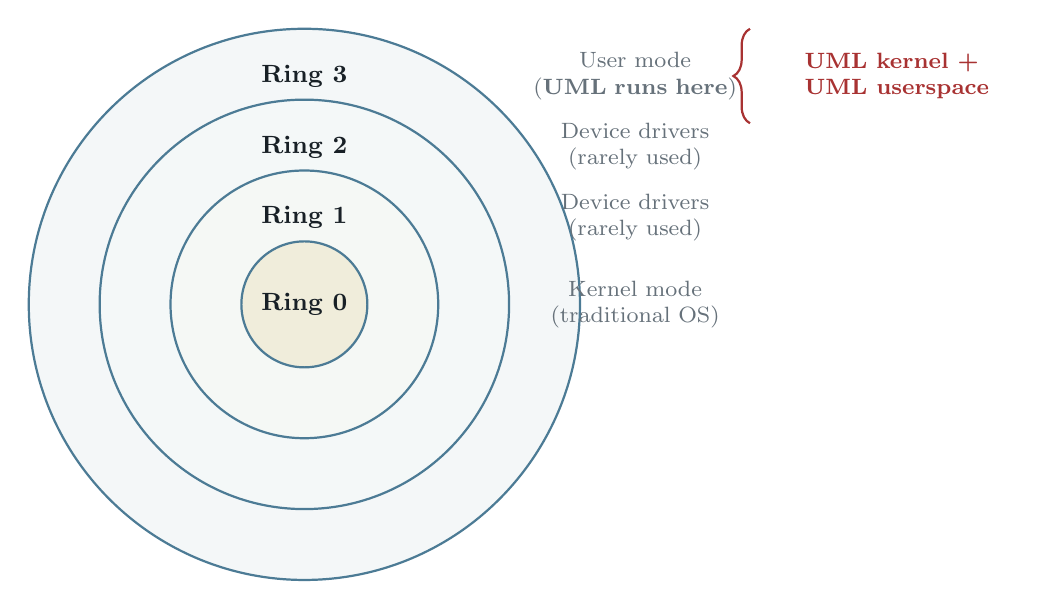
\begin{tikzpicture}[
  ring/.style={draw, thick, circle, minimum size=#1, color=UMLBlue!80},
  rlabel/.style={font=\small\bfseries, color=UMLInk},
  desc/.style={font=\footnotesize, color=UMLMuted, text width=3.5cm, align=center}
]
  % Rings (outermost first for layering)
  \node[ring=7.0cm, fill=UMLBlue!5]  (r3) at (0,0) {};
  \node[ring=5.2cm, fill=UMLTeal!5]  (r2) at (0,0) {};
  \node[ring=3.4cm, fill=UMLGreen!5] (r1) at (0,0) {};
  \node[ring=1.6cm, fill=KernelGold!15] (r0) at (0,0) {};

  % Labels
  \node[rlabel] at (0,0)    {Ring 0};
  \node[rlabel] at (0,1.1)  {Ring 1};
  \node[rlabel] at (0,2.0)  {Ring 2};
  \node[rlabel] at (0,2.9)  {Ring 3};

  % Descriptions
  \node[desc] at (4.2, 0)    {Kernel mode\\(traditional OS)};
  \node[desc] at (4.2, 1.1)  {Device drivers\\(rarely used)};
  \node[desc] at (4.2, 2.0)  {Device drivers\\(rarely used)};
  \node[desc] at (4.2, 2.9)  {User mode\\(\textbf{UML runs here})};

  % Brace for UML
  \draw[decorate, decoration={brace, amplitude=6pt, raise=4pt},
        thick, UMLRed]
    (5.8, 2.3) -- (5.8, 3.5)
    node[midway, right=12pt, font=\footnotesize\bfseries, color=UMLRed,
         text width=2.5cm, align=left]
    {UML kernel +\\UML userspace};
\end{tikzpicture}
\caption{The x86 privilege ring model.  Traditional kernels occupy
Ring~0; \UML{} runs entirely at Ring~3 (CPL=3), sharing the same
privilege level as ordinary user processes.}
\label{fig:x86-rings}
\end{figure}

Traditional operating systems use a two-ring model: the kernel at
Ring~0, user processes at Ring~3.  Rings~1 and~2 exist in hardware
but are almost universally unused.\footnote{OS/2 and a few
microkernel-inspired designs briefly used Ring~1 or Ring~2 for device
drivers, but the x86-64 long mode effectively reduces the model to
two rings in practice.}

\subsection{Implications for UML}

\UML{} runs entirely at Ring~3.  This has several consequences:

\begin{enumerate}
  \item \textbf{No privileged instructions.}
        The \UML{} kernel cannot execute \texttt{cli}/\texttt{sti}
        (interrupt control), \texttt{mov~cr3} (page-table switching),
        \texttt{lgdt}/\texttt{lidt} (descriptor-table loading), or
        any other privileged instruction.  Every such operation must
        be emulated via host system calls.

  \item \textbf{No direct hardware access.}
        All I/O must pass through the host kernel's system-call
        interface.  \UML{}'s block driver issues \syscall{read}/\syscall{write}
        on a host file descriptor; its network driver uses host sockets
        or TUN/TAP devices.

  \item \textbf{Shared address space with the host.}
        The \UML{} process occupies the same 48-bit (or 57-bit) virtual
        address space managed by the host kernel.  The host kernel's
        own mappings (above the canonical hole) are inaccessible from
        CPL=3, but the host's ASLR layout, vDSO, and stack placement
        all constrain where \UML{} can place its own data structures.

  \item \textbf{System call interception required.}
        When guest userspace issues a \texttt{syscall} instruction, it
        would normally trap into the \emph{host} kernel, not the
        \UML{} kernel.  \UML{} must intercept this trap and redirect
        it to its own system-call handler.  The mechanism for this
        interception---\syscall{ptrace}, \Seccomp{}, or \KVM{}---is
        the defining architectural choice of each \UML{} backend.
\end{enumerate}


% ------------------------------------------------------------------
\section{Hardware Virtualization Extensions}
\label{sec:foundations:hwvirt}

The x86 architecture famously violates the Popek--Goldberg
requirements: several sensitive instructions (notably \texttt{popf},
\texttt{sgdt}, and \texttt{pushf}) are not privileged and therefore
do not trap when executed in user mode~\cite{adams2006}.  This made
software-only full virtualization on x86 difficult, requiring either
binary translation (VMware) or paravirtualization (Xen).

Hardware virtualization extensions---Intel VT-x (2005) and AMD-V
(2006)---solve this by adding a new, orthogonal dimension of privilege.

\subsection{Intel VT-x (VMX)}

VT-x~\cite{intel-sdm} introduces \textbf{VMX root mode} (the
hypervisor) and \textbf{VMX non-root mode} (the guest).  The
transition between the two is mediated by a per-vCPU data structure
called the \textbf{Virtual Machine Control Structure} (VMCS):

\begin{description}[style=nextline]
  \item[VM Entry (\texttt{VMLAUNCH} / \texttt{VMRESUME}).]
    The hypervisor loads guest state from the VMCS and transfers
    control to the guest.  The guest runs at whatever CPL the VMCS
    guest-state area specifies---typically Ring~0 for a full-system
    guest, or Ring~3 for a process-level guest like \UML{}'s \KVM{}
    backend.

  \item[VM Exit.]
    Certain events cause the processor to stop guest execution,
    save guest state into the VMCS, and transfer control back to
    VMX root mode.  The exit reason is recorded in the VMCS.
    Events that cause exits include: execution of privileged
    instructions, I/O instructions (if the I/O bitmap so indicates),
    external interrupts, page faults (if configured), and the
    \texttt{CPUID} instruction.

  \item[Extended Page Tables (EPT).]
    EPT provides a second level of address translation: guest-physical
    addresses (GPAs) are translated to host-physical addresses (HPAs)
    by hardware, without any hypervisor intervention for non-faulting
    accesses.  This eliminates the ``shadow page table'' overhead that
    made pre-EPT virtualization expensive.
\end{description}

\subsection{AMD-V (SVM)}

AMD's Secure Virtual Machine~\cite{amd-apm} follows the same
principles with different terminology: the per-vCPU structure is the
\textbf{Virtual Machine Control Block} (VMCB); the hardware nested
paging feature is called \textbf{Nested Page Tables} (NPT); and the
entry/exit instructions are \texttt{VMRUN} and---implicitly---any
intercepted event.  The functional model is equivalent for the
purposes of this report.

\subsection{KVM and the ioctl Interface}

\KVM{}~\cite{kivity2007} exposes hardware virtualization to userspace
through a layered ioctl interface on \texttt{/dev/kvm}:

\begin{enumerate}
  \item \texttt{KVM\_CREATE\_VM} returns a VM file descriptor.
  \item \texttt{KVM\_SET\_USER\_MEMORY\_REGION} on the VM fd maps
        host-virtual memory into the guest-physical address space
        (backing EPT/NPT).
  \item \texttt{KVM\_CREATE\_VCPU} on the VM fd returns a vCPU file
        descriptor, with a shared \texttt{struct kvm\_run} page
        accessible via \syscall{mmap} on the vCPU fd.
  \item \texttt{KVM\_RUN} on the vCPU fd enters VMX/SVM non-root mode.
        When the guest causes an exit, \texttt{KVM\_RUN} returns and
        the exit reason + auxiliary data are available in the shared
        \texttt{kvm\_run} page.
\end{enumerate}

\subsection{Why This Matters for UML}

\UML{}'s \KVM{} backend uses this interface to run guest code at
Ring~3 \emph{inside a virtual machine}, while the \UML{} kernel
process remains an ordinary userspace process on the host.  The
critical insight is that \KVM{}'s VM entry/exit cycle is far cheaper
than a \syscall{ptrace} round-trip or even a \Seccomp{} SIGSYS
delivery.  A \texttt{KVM\_RUN} $\rightarrow$ \texttt{KVM\_EXIT\_IO}
round-trip costs approximately \SIrange{100}{150}{\nano\second}; with
the LSTAR gadget (Section~\ref{sec:foundations:trap-compare}), trivial
system calls complete in approximately 90 cycles without exiting the
VM at all.


% ------------------------------------------------------------------
\section{The Linux Process Model}
\label{sec:foundations:process-model}

From the host kernel's perspective, a running \UML{} instance is an
ordinary multi-threaded process (or set of processes, depending on the
backend).  \UML{} exploits a specific set of Linux system calls to
implement its virtualization layer.

\subsection{ptrace: The Original Trap Mechanism}

The \syscall{ptrace} system call~\cite{ptrace-man} allows one process
(the \emph{tracer}) to observe and control the execution of another
(the \emph{tracee}).  \UML{}'s original backend uses:

\begin{description}[style=nextline]
  \item[\texttt{PTRACE\_SYSEMU}.]
    Resumes the tracee but intercepts the next system call
    \emph{without executing it}.  The tracee stops with a
    \texttt{SIGTRAP|0x80} signal.  This is the key extension that
    Jeff Dike contributed to the Linux kernel specifically for
    \UML{}: without it, the host kernel would execute the guest's
    system call before \UML{} could intercept it.

  \item[\texttt{PTRACE\_GETREGS} / \texttt{PTRACE\_SETREGS}.]
    Read and write the tracee's general-purpose registers.  \UML{}
    reads the registers to determine which system call the guest
    requested (from \texttt{RAX}) and its arguments (from
    \texttt{RDI}, \texttt{RSI}, \texttt{RDX}, \texttt{R10},
    \texttt{R8}, \texttt{R9} per the x86-64 ABI), then writes the
    return value back into \texttt{RAX}.
\end{description}

\subsection{seccomp: The Modern Trap Mechanism}

The \Seccomp{} BPF filter~\cite{seccomp-bpf} was originally designed
for sandboxing (Chrome, Firefox, container runtimes), but its
\texttt{SECCOMP\_RET\_TRAP} return action proved ideal for \UML{}.
When a seccomp filter returns \texttt{SECCOMP\_RET\_TRAP}, the kernel
delivers a \texttt{SIGSYS} signal to the thread that issued the
system call---without executing it.  This is functionally equivalent
to \texttt{PTRACE\_SYSEMU} but with dramatically lower overhead
because the signal is delivered in-process rather than requiring a
context switch to an external tracer.

\subsection{futex: Stub Synchronization}

The \syscall{futex} system call provides efficient userspace-to-kernel
synchronization~\cite{futex-lwn}.  In the \Seccomp{} backend, the
stub process and the \UML{} kernel use a shared \texttt{futex} word
(in the \texttt{stub\_data} page) to implement a lightweight turnstile:
the stub writes its trap state, issues \texttt{FUTEX\_WAKE}, and blocks
on \texttt{FUTEX\_WAIT}; the \UML{} kernel wakes, processes the trap,
writes the result, and wakes the stub.

\subsection{mmap / munmap / mprotect: Guest Memory}

\UML{} implements guest ``physical'' memory as a host-side anonymous
mapping or a file-backed mapping (typically on \texttt{tmpfs}).  Guest
page-table changes are realized by calling \syscall{mmap},
\syscall{munmap}, and \syscall{mprotect} on the host to adjust the
stub process's address space.  Each guest TLB flush translates to a
batch of these host system calls.

\subsection{clone / fork: Guest Processes}

Each guest process in \UML{} is backed by a host process (or thread,
depending on the configuration).  The \syscall{clone} system call
creates the host-side entity; \texttt{CLONE\_VM} may or may not be
used depending on whether the backend shares address spaces.

\subsection{KVM ioctl Interface}
\label{sec:foundations:kvm-api}

The \KVM{} backend~\cite{kvm-api} replaces the \syscall{ptrace} and
\Seccomp{} trap mechanisms with hardware-assisted virtualization.  The
key ioctls are:

\begin{lstlisting}[language=KernelC,caption={KVM ioctl sequence for
UML's v2 backend.},label=lst:kvm-ioctls]
/* VM creation (once per UML instance) */
vm_fd = ioctl(kvm_fd, KVM_CREATE_VM, 0);

/* Map guest physical memory (host tmpfs -> guest GPA) */
struct kvm_userspace_memory_region mem = {
    .slot            = 0,
    .guest_phys_addr = 0,
    .memory_size     = physmem_size,
    .userspace_addr  = (u64)uml_physmem,
};
ioctl(vm_fd, KVM_SET_USER_MEMORY_REGION, &mem);

/* Per-vCPU creation (one per host CPU in the pool) */
vcpu_fd = ioctl(vm_fd, KVM_CREATE_VCPU, cpu_id);
run = mmap(NULL, sizeof(struct kvm_run), PROT_RW,
           MAP_SHARED, vcpu_fd, 0);

/* Hot loop: enter guest, handle exit, re-enter */
while (1) {
    ioctl(vcpu_fd, KVM_RUN, 0);
    switch (run->exit_reason) {
    case KVM_EXIT_IO:
        handle_io_trap(regs, run, vcpu);
        break;
    /* ... other exit reasons ... */
    }
}
\end{lstlisting}


% ------------------------------------------------------------------
\section{Address Space Layout}
\label{sec:foundations:address-space}

\UML{} must carve a complete kernel and user address space out of the
host process's available virtual address range.  The layout differs
between the \Seccomp{} and \KVM{} backends.

\begin{figure}[ht]
\centering
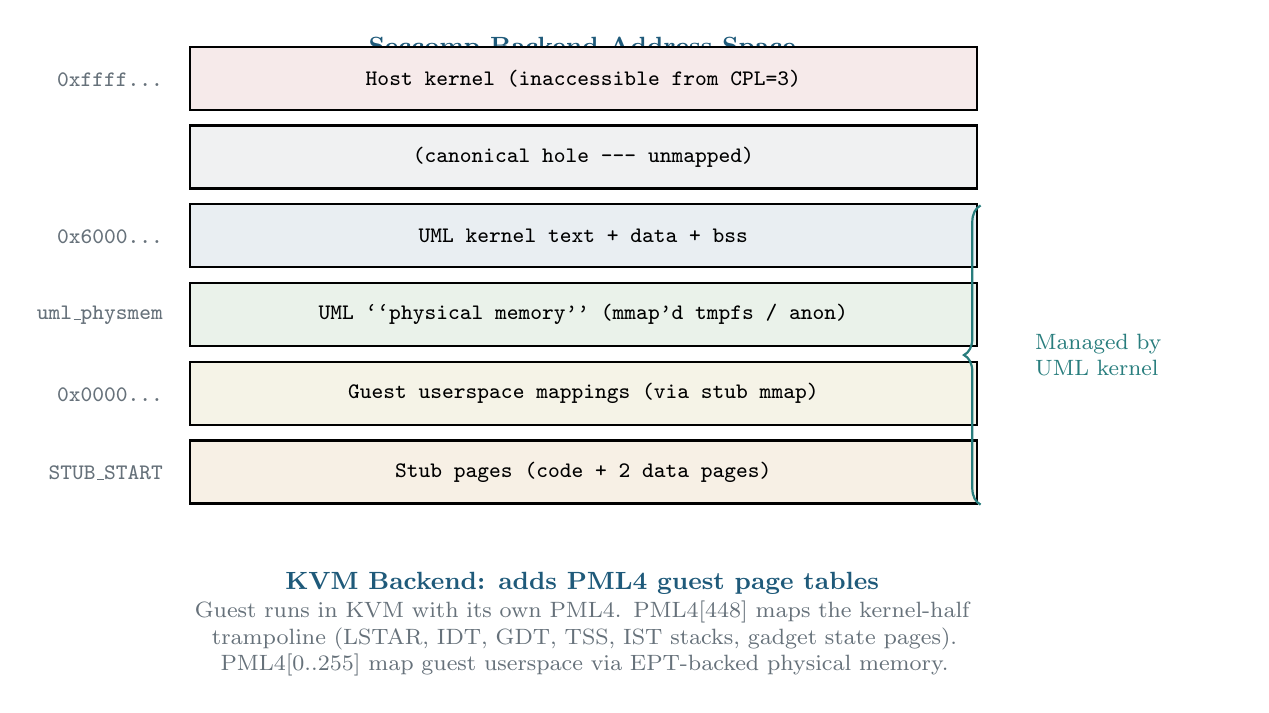
\begin{tikzpicture}[
  block/.style={draw, thick, minimum width=10cm, minimum height=0.8cm,
                font=\footnotesize\ttfamily, anchor=south west},
  label/.style={font=\footnotesize, color=UMLMuted, anchor=east},
  >=Stealth
]
  % Seccomp layout
  \node[font=\small\bfseries, color=UMLBlue] at (5, 7.8) {Seccomp Backend Address Space};

  \node[block, fill=UMLRed!10]    (hk) at (0, 7)
    {Host kernel (inaccessible from CPL=3)};
  \node[label] at (-0.2, 7.4) {\texttt{0xffff...}};

  \node[block, fill=UMLMuted!10]  (gap1) at (0, 6)
    {(canonical hole --- unmapped)};

  \node[block, fill=UMLBlue!10]   (ukt) at (0, 5)
    {UML kernel text + data + bss};
  \node[label] at (-0.2, 5.4) {\texttt{0x6000...}};

  \node[block, fill=UMLGreen!10]  (phys) at (0, 4)
    {UML ``physical memory'' (mmap'd tmpfs / anon)};
  \node[label] at (-0.2, 4.4) {\texttt{uml\_physmem}};

  \node[block, fill=KernelGold!10] (guest) at (0, 3)
    {Guest userspace mappings (via stub mmap)};
  \node[label] at (-0.2, 3.4) {\texttt{0x0000...}};

  \node[block, fill=UMLAmber!10]  (stub) at (0, 2)
    {Stub pages (code + 2 data pages)};
  \node[label] at (-0.2, 2.4) {\texttt{STUB\_START}};

  \draw[decorate, decoration={brace, amplitude=6pt, raise=4pt},
        thick, UMLTeal]
    (10.2, 2) -- (10.2, 5.8)
    node[midway, right=12pt, font=\footnotesize, color=UMLTeal,
         text width=2.5cm, align=left]
    {Managed by\\UML kernel};

  % KVM layout annotation
  \node[font=\small\bfseries, color=UMLBlue] at (5, 1.0) {KVM Backend: adds PML4 guest page tables};
  \node[font=\footnotesize, color=UMLMuted, text width=10cm, align=center] at (5, 0.3)
    {Guest runs in KVM with its own PML4. PML4[448] maps the kernel-half\\
     trampoline (LSTAR, IDT, GDT, TSS, IST stacks, gadget state pages).\\
     PML4[0..255] map guest userspace via EPT-backed physical memory.};
\end{tikzpicture}
\caption{Address space layout for the \Seccomp{} backend.  The \KVM{}
backend additionally constructs guest-side PML4 page tables
that map the same physical memory through EPT/NPT.}
\label{fig:address-space}
\end{figure}

\subsection{Seccomp Backend Layout}

The \Seccomp{} backend's stub process has the following regions in its
virtual address space (Figure~\ref{fig:address-space}):

\begin{enumerate}
  \item \textbf{Guest userspace} (\texttt{0x0} to approximately
        \texttt{TASK\_SIZE}).  Mapped by the \UML{} kernel via batched
        \syscall{mmap}/\syscall{mprotect} calls into the stub process.

  \item \textbf{Stub pages} (\texttt{STUB\_START} to \texttt{STUB\_END}).
        Three pages: one page of stub executable code (the \texttt{SIGSYS}
        handler, the \syscall{futex} wait/wake loop, the syscall-batch
        executor) and two pages of \texttt{stub\_data} (shared state:
        registers, signal information, the futex word, and the
        syscall-batch buffer).

  \item \textbf{UML physical memory} (\texttt{uml\_physmem}).
        The contiguous region backing guest RAM, typically \syscall{mmap}'d
        from a \texttt{tmpfs} file descriptor or as anonymous memory.
        Guest page tables reference offsets within this region.

  \item \textbf{UML kernel text/data.}  The \UML{} binary's own code
        and data segments, loaded by the host's ELF loader.
\end{enumerate}

\subsection{KVM Backend: Guest Page Tables}

The \KVM{} backend constructs a full x86-64 PML4 page-table hierarchy
for the guest.  \UML{}'s physical memory is registered with \KVM{}
via \texttt{KVM\_SET\_USER\_MEMORY\_REGION}, which populates EPT/NPT
entries so that guest-physical addresses translate through host-virtual
addresses to host-physical pages without hypervisor intervention on
each access.

The guest PML4 contains a \emph{kernel half} at PML4 slot~448
(guest virtual address \texttt{0xffffe000\_00000000}) that maps the
trampoline page (LSTAR entry point), the IDT, exception handler stubs,
the GDT, per-vCPU TSS and IST stack pages, and per-vCPU gadget state
pages.  This kernel-half mapping is marked \texttt{US=0}
(supervisor-only) so guest userspace at CPL=3 cannot access it
directly; the CPU transitions to CPL=0 only transiently during the
\texttt{SYSCALL} instruction's microarchitectural handling before the
LSTAR trampoline code runs.


% ------------------------------------------------------------------
\section{Trap Mechanisms Compared}
\label{sec:foundations:trap-compare}

The performance of \UML{} is dominated by the cost of intercepting
guest system calls.  Three mechanisms have been used historically and
in the current implementation.  Figure~\ref{fig:trap-paths} illustrates
the data flow for each.

\subsection{ptrace: PTRACE\_SYSEMU}

The original \UML{} trap mechanism uses \syscall{ptrace} to intercept
every guest system call:

\begin{enumerate}
  \item Guest userspace executes the \texttt{syscall} instruction.
  \item The host kernel intercepts it (via \texttt{PTRACE\_SYSEMU})
        and stops the tracee with signal \texttt{SIGTRAP|0x80}.
  \item The \UML{} kernel (the tracer) wakes from \syscall{waitpid}.
  \item \texttt{PTRACE\_GETREGS} reads the tracee's register state.
  \item The \UML{} kernel dispatches the appropriate handler.
  \item \texttt{PTRACE\_SETREGS} writes the return value.
  \item \texttt{PTRACE\_SYSEMU} resumes the tracee.
\end{enumerate}

Each round-trip requires two context switches between the tracer and
the tracee plus multiple kernel transitions.  Measured latency:
\textbf{\SIrange{1}{5}{\micro\second}} per system call.

\subsection{seccomp: SIGSYS + futex}

The \Seccomp{} backend (contributed by Johannes Berg, circa 2022)
replaces the external-tracer model with an in-process signal:

\begin{enumerate}
  \item Guest userspace executes the \texttt{syscall} instruction.
  \item The host kernel's seccomp filter returns
        \texttt{SECCOMP\_RET\_TRAP}, delivering \texttt{SIGSYS} to
        the stub thread---\emph{without executing the system call}.
  \item The stub's \texttt{SIGSYS} handler saves register state into
        the shared \texttt{stub\_data} page.
  \item The stub issues \texttt{FUTEX\_WAKE} on the shared futex word,
        waking the \UML{} kernel thread.
  \item The \UML{} kernel reads registers from \texttt{stub\_data},
        dispatches the handler, and writes the result back.
  \item The \UML{} kernel issues \texttt{FUTEX\_WAKE}; the stub wakes
        from its \texttt{FUTEX\_WAIT} and resumes guest execution from
        the signal return path.
\end{enumerate}

Because no external tracer is involved, the context-switch overhead is
eliminated.  The signal delivery and futex round-trip are the dominant
costs.  Measured latency: \textbf{\SIrange{300}{500}{\nano\second}}
per system call---roughly an order of magnitude faster than \syscall{ptrace}.

\subsection{KVM: vmentry/vmexit + LSTAR Gadget}

The \KVM{} backend replaces the signal-based mechanism with hardware
VM entry/exit:

\begin{enumerate}
  \item Guest userspace executes the \texttt{syscall} instruction.
  \item The CPU loads \texttt{MSR\_LSTAR} into RIP (standard x86-64
        \texttt{SYSCALL} behavior).  Inside the guest VM, LSTAR points
        to the \UML{} trampoline page.
  \item The LSTAR trampoline executes \texttt{out \%al, \$0xf4}
        (an I/O instruction on port \texttt{0xf4}).
  \item The I/O instruction causes a \texttt{KVM\_EXIT\_IO} VM exit.
  \item The \UML{} kernel (running in VMX root mode via the
        \texttt{KVM\_RUN} return path) reads the exit reason, extracts
        registers from the shared \texttt{kvm\_run} page, and dispatches
        the system-call handler.
  \item The handler writes the return value into \texttt{kvm\_run},
        and the next \texttt{KVM\_RUN} call re-enters the guest.
        The guest resumes via \texttt{sysretq} from the trampoline.
\end{enumerate}

Measured latency for the full round-trip:
\textbf{\SIrange{100}{150}{\nano\second}} per system call.

\subsubsection{The LSTAR Gadget: Avoiding the Exit Entirely}

For a curated set of trivial system calls (\syscall{getpid},
\syscall{gettid}, \syscall{getppid}, \syscall{getuid},
\syscall{geteuid}, \syscall{getgid}, \syscall{getegid},
\syscall{getcpu}, \syscall{time}, and
\texttt{clock\_gettime(CLOCK\_MONOTONIC)}), the LSTAR trampoline
contains an expanded 343-byte \emph{gadget} that handles the system
call entirely within the guest, without any VM exit:

\begin{enumerate}
  \item \texttt{swapgs} switches GS base to a per-vCPU state page
        populated by the host on each context switch.
  \item A dispatch chain (\texttt{cmp}/\texttt{je} on the syscall
        number in \texttt{EAX}) routes to the appropriate handler.
  \item The handler reads the pre-computed return value from the
        per-vCPU state page via \texttt{\%gs:offset}.
  \item \texttt{swapgs} + \texttt{sysretq} returns directly to guest
        userspace.
\end{enumerate}

The entire sequence---including the \texttt{SYSCALL}/\texttt{SYSRET}
pair---completes in approximately \textbf{90~cycles} ($\approx$
\SI{30}{\nano\second} at \SI{3}{\giga\hertz}).  For workloads that
call \syscall{getpid} or \texttt{clock\_gettime} in tight loops, this
approaches bare-metal performance.

\begin{figure}[ht]
\centering
\begin{tikzpicture}[
  box/.style={draw, thick, rounded corners=3pt, minimum height=0.7cm,
              font=\footnotesize, text width=2.3cm, align=center},
  arrow/.style={-{Stealth[length=5pt]}, thick},
  phase/.style={font=\footnotesize\bfseries, color=UMLBlue},
  timing/.style={font=\scriptsize\itshape, color=UMLRed}
]
  % ptrace path
  \node[phase] at (-1.5, 5.5) {ptrace};
  \node[box, fill=KernelGold!15] (p1) at (0, 5) {Guest\\syscall};
  \node[box, fill=UMLRed!10]     (p2) at (3, 5) {Host kernel\\SYSEMU stop};
  \node[box, fill=UMLBlue!10]    (p3) at (6, 5) {waitpid\\GETREGS};
  \node[box, fill=UMLGreen!10]   (p4) at (9, 5) {UML\\handler};
  \node[box, fill=UMLBlue!10]    (p5) at (12, 5) {SETREGS\\SYSEMU};
  \draw[arrow] (p1) -- (p2);
  \draw[arrow] (p2) -- (p3);
  \draw[arrow] (p3) -- (p4);
  \draw[arrow] (p4) -- (p5);
  \draw[arrow, dashed] (p5) .. controls (14, 5) and (14, 5.8) ..
    (12.5, 5.8) -- (-0.5, 5.8) .. controls (-2, 5.8) and (-2, 5) .. (p1);
  \node[timing] at (6, 4.3) {$\sim$1--5 \textmu{}s per syscall};

  % seccomp path
  \node[phase] at (-1.5, 3.0) {seccomp};
  \node[box, fill=KernelGold!15] (s1) at (0, 2.5) {Guest\\syscall};
  \node[box, fill=UMLAmber!10]   (s2) at (3, 2.5) {SIGSYS\\handler};
  \node[box, fill=UMLTeal!10]    (s3) at (6, 2.5) {futex wake\\UML kernel};
  \node[box, fill=UMLGreen!10]   (s4) at (9, 2.5) {UML\\handler};
  \node[box, fill=UMLTeal!10]    (s5) at (12, 2.5) {futex wake\\stub};
  \draw[arrow] (s1) -- (s2);
  \draw[arrow] (s2) -- (s3);
  \draw[arrow] (s3) -- (s4);
  \draw[arrow] (s4) -- (s5);
  \draw[arrow, dashed] (s5) .. controls (14, 2.5) and (14, 3.3) ..
    (12.5, 3.3) -- (-0.5, 3.3) .. controls (-2, 3.3) and (-2, 2.5) .. (s1);
  \node[timing] at (6, 1.8) {$\sim$300--500 ns per syscall};

  % KVM path
  \node[phase] at (-1.5, 0.5) {KVM};
  \node[box, fill=KernelGold!15] (k1) at (0, 0) {Guest\\SYSCALL};
  \node[box, fill=UMLAmber!15]   (k2) at (3, 0) {LSTAR\\out \$0xf4};
  \node[box, fill=UMLRed!10]     (k3) at (6, 0) {KVM\_EXIT\\\_IO};
  \node[box, fill=UMLGreen!10]   (k4) at (9, 0) {UML\\handler};
  \node[box, fill=UMLBlue!10]    (k5) at (12, 0) {KVM\_RUN\\re-enter};
  \draw[arrow] (k1) -- (k2);
  \draw[arrow] (k2) -- (k3);
  \draw[arrow] (k3) -- (k4);
  \draw[arrow] (k4) -- (k5);
  \draw[arrow, dashed] (k5) .. controls (14, 0) and (14, 0.8) ..
    (12.5, 0.8) -- (-0.5, 0.8) .. controls (-2, 0.8) and (-2, 0) .. (k1);
  \node[timing] at (6, -0.7) {$\sim$100--150 ns per syscall
    (gadget: $\sim$90 cycles, no exit)};
\end{tikzpicture}
\caption{System call interception paths for the three \UML{} trap
mechanisms.  Dashed arrows show the return-to-guest path.}
\label{fig:trap-paths}
\end{figure}

\subsection{Comparison Table}

\begin{table}[ht]
\centering
\caption{Trap mechanism comparison.  Latencies are representative
measurements for a null system call (e.g., \syscall{getpid}) on
contemporary hardware (Intel Alder Lake / AMD Zen~4, 2024--2026).}
\label{tab:trap-comparison}
\small
\begin{tabularx}{\textwidth}{@{} l Y Y Y @{}}
\toprule
\textbf{Property} &
  \textbf{ptrace} &
  \textbf{seccomp} &
  \textbf{KVM (v2)} \\
\midrule
Trap mechanism &
  \texttt{PTRACE\_SYSEMU} $\rightarrow$ \texttt{SIGTRAP|0x80} &
  \texttt{SECCOMP\_RET\_TRAP} $\rightarrow$ \texttt{SIGSYS} &
  \texttt{SYSCALL} $\rightarrow$ LSTAR $\rightarrow$ \texttt{out} $\rightarrow$ \texttt{KVM\_EXIT\_IO} \\
\midrule
Syscall latency &
  \SIrange{1}{5}{\micro\second} &
  \SIrange{300}{500}{\nano\second} &
  \SIrange{100}{150}{\nano\second} \\
\midrule
Gadget fast-path &
  N/A &
  N/A &
  $\sim$90 cycles ($\sim$\SI{30}{\nano\second}), no VM exit \\
\midrule
Context switches &
  2 per syscall (tracer $\leftrightarrow$ tracee) &
  0 (in-process signal) &
  1 VM exit + 1 VM entry \\
\midrule
Host kernel requirement &
  \texttt{PTRACE\_SYSEMU} support &
  \texttt{SECCOMP\_RET\_TRAP} (kernel $\geq$ 3.5) &
  \texttt{/dev/kvm} + VT-x/AMD-V \\
\midrule
Guest memory model &
  \syscall{mmap} into stub process &
  \syscall{mmap} into stub process &
  \texttt{KVM\_SET\_USER\_MEMORY\_REGION} (EPT/NPT) \\
\midrule
SMP model &
  One host process per guest CPU &
  One host thread per guest CPU &
  One vCPU per host CPU (pool) \\
\midrule
Debugging support &
  Full ptrace attach &
  Limited (signal-based) &
  \texttt{KVM\_GUESTDBG\_*} (breakpoints, single-step) \\
\midrule
Kernel version in-tree &
  v2.4.x -- present (mainline) &
  v6.1 -- present (Berg series) &
  v2 in development (this work) \\
\bottomrule
\end{tabularx}
\end{table}


% ------------------------------------------------------------------
\section{Memory Management Under UML}
\label{sec:foundations:memory}

\subsection{Guest Physical Memory}

\UML{}'s ``physical memory'' is a contiguous host-virtual region of
size \texttt{physmem\_size} (set by the \texttt{mem=} boot parameter,
default \SI{64}{\mebi\byte}).  It is backed either by a file on
\texttt{tmpfs} (the traditional approach) or by an anonymous
\texttt{MAP\_PRIVATE} mapping.  The file-backed approach supports
\texttt{MAP\_SHARED} semantics, enabling host-side inspection of
guest memory; the anonymous approach avoids filesystem overhead.

Guest physical addresses are simple offsets into this region:
\begin{equation*}
  \text{host\_va}(\text{gpa}) = \texttt{uml\_physmem} + \text{gpa}
\end{equation*}

\subsection{Guest Page Tables}

\UML{} maintains full x86-64 four-level page tables (PML4 $\rightarrow$
PDP $\rightarrow$ PD $\rightarrow$ PT) in guest physical memory.  These
page tables serve different purposes depending on the backend:

\begin{description}[style=nextline]
  \item[Seccomp/ptrace backends.]
    Guest page tables exist only as a data structure internal to the
    \UML{} kernel.  They record the guest's virtual-to-physical
    mappings, but the \emph{actual} address translation is performed
    by the host kernel's page tables (the stub process's
    \texttt{mm\_struct}).  When the guest modifies a PTE, \UML{} must
    call \syscall{mmap}/\syscall{mprotect} on the stub process to
    make the host-side mapping match.

  \item[KVM backend.]
    Guest page tables are loaded into the vCPU's CR3 and walked by
    hardware during guest execution.  EPT/NPT provides the second
    level of translation (guest-physical to host-physical).  \UML{}
    still maintains the guest page tables as data structures, but
    they are now \emph{live}---the CPU reads them directly.
\end{description}

\subsection{The TLB Synchronization Problem}
\label{sec:foundations:tlb-sync}

When the \UML{} kernel modifies a guest page-table entry---due to a
page fault, an \syscall{mmap}, an \syscall{mprotect}, or a process
exit---the change must be propagated to the execution substrate:

\begin{description}[style=nextline]
  \item[Seccomp backend:]
    Each PTE change is translated into a host \syscall{mmap} or
    \syscall{mprotect} call, batched into the stub's syscall buffer
    (\texttt{stub\_data->syscall\_data}), and flushed on the next
    stub round-trip.  This is the \texttt{um\_tlb\_sync()} path in
    \umlpath{arch/um/kernel/tlb.c}.

  \item[KVM backend:]
    PTE changes are written directly into the guest page-table pages
    (which live in \UML{}'s physical memory region).  The \UML{} kernel
    then issues \texttt{INVLPG} or a full CR3 reload within the guest
    to invalidate stale TLB entries.  On SMP configurations,
    \texttt{tlb\_kick\_others()} sends an IPI to force all other vCPUs
    to flush their TLBs as well---this is the \KVM{}-specific backend
    op that the \Seccomp{} backend leaves NULL (the host kernel's
    mmu\_notifier mechanism handles cross-CPU invalidation
    transparently for the \Seccomp{} path).
\end{description}

The TLB sync path is one of the most performance-sensitive operations
in \UML{}.  The \Seccomp{} backend batches multiple PTE changes into
a single stub round-trip (amortizing the futex wake/wait overhead over
dozens of mappings), while the \KVM{} backend avoids host system calls
entirely for the common case, paying only the cost of a guest-side
\texttt{INVLPG} or CR3 write.


% ------------------------------------------------------------------
\section{Signal Handling}
\label{sec:foundations:signals}

Signals are the ``interrupts'' of the \UML{} kernel.  Where a
bare-metal kernel receives timer ticks via a local APIC interrupt and
I/O notifications via device IRQs, \UML{} receives:

\begin{description}[style=nextline]
  \item[\texttt{SIGALRM}:]
    Timer interrupts.  The \UML{} kernel programs a host
    \texttt{timer\_create}/\texttt{timer\_settime} timer (or
    \texttt{setitimer} on older configurations) that delivers
    \texttt{SIGALRM} at the frequency required by the guest's
    \texttt{HZ} setting.  This drives the scheduler tick, watchdog
    timers, and all time-dependent kernel subsystems.

  \item[\texttt{SIGIO}:]
    I/O readiness notifications.  \UML{}'s virtual device drivers
    register host file descriptors with the \UML{} IRQ subsystem,
    which uses \texttt{epoll} (or \texttt{poll}) and arranges for
    \texttt{SIGIO} delivery when any registered descriptor becomes
    ready.  This is the functional equivalent of a hardware IRQ
    line going active.

  \item[\texttt{SIGSEGV}:]
    Page faults.  When guest code accesses an address that is not
    mapped in the stub process's host-side page tables (for the
    \Seccomp{} backend) or that causes an EPT violation (for the
    \KVM{} backend), the resulting fault is delivered to the \UML{}
    kernel, which resolves it by consulting the guest page tables,
    allocating physical pages if necessary, and updating the mapping.

  \item[\texttt{SIGSYS}:]
    System call interception (\Seccomp{} backend only).  As described
    in Section~\ref{sec:foundations:trap-compare}, the seccomp filter's
    \texttt{SECCOMP\_RET\_TRAP} action delivers this signal to indicate
    that the guest issued a system call.
\end{description}

\subsection{Signal Delivery Across Backends}

The signal model differs substantially between backends:

\begin{itemize}
  \item \textbf{Seccomp backend:}
    \texttt{SIGALRM} and \texttt{SIGIO} are delivered asynchronously
    to the \UML{} kernel thread (the ``spawner'' process or the per-mm
    worker process).  The signal handler runs in the \UML{} kernel's
    context, interrupting whatever kernel code was executing.  Signal
    masking ensures that only one signal is handled at a time.

  \item \textbf{KVM backend:}
    While a vCPU is inside \texttt{KVM\_RUN}, host signals cannot be
    delivered to the thread---the thread is in kernel space executing
    the KVM entry/exit loop.  Instead, pending signals cause
    \texttt{KVM\_RUN} to return with \texttt{-EINTR} (or, with
    signal-window-based delivery, the signal is handled before the
    next \texttt{KVM\_RUN} call).  The \UML{} kernel's vCPU run loop
    checks for pending signals after each VM exit and dispatches
    them through the standard \UML{} interrupt-handling path.

    This means \texttt{SIGALRM} timer ticks are effectively ``held''
    during guest execution and processed at the next VM exit
    boundary.  For the LSTAR gadget fast path, which handles system
    calls without any VM exit, this creates a timer-delivery gap:
    a tight loop calling only gadget-handled system calls could
    theoretically starve the timer.  The gadget's \emph{budget}
    mechanism addresses this: each gadget-handled
    \texttt{clock\_gettime} call decrements a per-vCPU budget counter,
    and when the budget reaches zero, the gadget falls back to the
    full VM exit path, ensuring the host has an opportunity to deliver
    pending signals.
\end{itemize}

\subsection{Signal Masking and Reentrancy}

\UML{}'s signal handlers must be carefully written to avoid reentrancy
issues.  The \UML{} kernel uses \texttt{sigprocmask} to block signals
during critical sections (analogous to \texttt{local\_irq\_disable()}
on bare metal) and unblocks them at safe points (analogous to
\texttt{local\_irq\_enable()}).  The \texttt{block\_signals\_trace()} /
\texttt{unblock\_signals\_trace()} wrappers in
\umlpath{arch/um/os-Linux/signal.c} implement this protocol, and all
signal-handler dispatchers use them to ensure that a \texttt{SIGALRM}
arriving during \texttt{SIGIO} handling (or vice versa) is deferred
rather than creating a nested handler invocation that could corrupt
kernel state.

\bigskip

With these foundations established---the virtualization taxonomy, the
x86 privilege model, hardware virtualization extensions, the Linux
process model, address-space layout, trap mechanisms, memory
management, and signal handling---we are now equipped to examine the
architecture of \UML{} itself in Chapter~\ref{ch:architecture}.

% ==========================================================================
%  Chapter 4 — UML Architecture and Design
% ==========================================================================
\chapter{UML Architecture and Design}
\label{ch:architecture}

\epigraph{%
  Every architecture port is a negotiation between the abstractions the kernel
  expects and the mechanisms the hardware provides.  In UML, the ``hardware''
  is another kernel.%
}{Author's observation}

User-Mode Linux is, at its core, an architecture port.  It implements the same
interfaces that \texttt{arch/x86}, \texttt{arch/arm64}, or \texttt{arch/riscv}
implement---trap dispatch, context switching, page table management, timer
infrastructure, SMP synchronization---but the target ``hardware'' is not a CPU
in ring~0.  It is the host Linux kernel, accessed through system calls.  This
chapter describes the internal architecture of the \texttt{arch/um/} tree as it
stands after the v2 redesign: the directory layout, the three-layer abstraction
model, the backend selection mechanism, the stub process model, guest memory
management, symmetric multiprocessing, the device model, and the build system.


% --------------------------------------------------------------------------
\section{The \texttt{arch/um/} Directory}
\label{sec:arch-um-dir}

In the Linux source tree, every supported architecture lives under a dedicated
subdirectory of \texttt{arch/}.  UML is no exception: \texttt{arch/um/}
contains roughly 40{,}000 lines of C (excluding tests and the archived v1 KVM
backend) spread across six major subdirectories and their associated headers.
What makes UML special is that the ``hardware abstraction layer'' at the bottom
of this code does not talk to PCI buses, interrupt controllers, or MMU hardware.
Instead it calls \syscall{clone}, \syscall{mmap}, \syscall{mprotect},
\syscall{futex}, \syscall{ioctl}, and \syscall{sigaction} on the host
kernel~\cite{dike2000,dike2006book}.

\subsection{Directory Structure}

Table~\ref{tab:arch-um-dirs} summarizes the top-level layout.  Two features of
this structure deserve emphasis.

\begin{table}[ht]
\centering
\caption{Top-level directories under \texttt{arch/um/}.}
\label{tab:arch-um-dirs}
\rowcolors{2}{UMLPanel}{white}
\begin{tabularx}{\textwidth}{l Y}
\toprule
\textbf{Directory} & \textbf{Purpose} \\
\midrule
\texttt{kernel/}   & Core kernel-side logic: trap dispatch (\texttt{trap.c}),
                      TLB synchronization (\texttt{tlb.c}), SMP
                      (\texttt{smp.c}), timekeeping (\texttt{time.c}), backend
                      arbiter (\texttt{backend.c}), Layer~2 static-key hooks
                      (\texttt{hooks.c}, \texttt{hooks\_bench.c}), template
                      pause (\texttt{template\_pause.c}), process management
                      (\texttt{process.c}), and the linker script
                      (\texttt{vmlinux.lds.S}). \\
\texttt{os-Linux/} & Host-side userspace code: signal handling
                      (\texttt{signal.c}), memory operations (\texttt{mem.c}),
                      process management (\texttt{process.c}), SMP pthread
                      lifecycle (\texttt{smp.c}), startup and probe
                      (\texttt{start\_up.c}), and the \texttt{skas/}
                      subdirectory containing the SKAS trap loop
                      (\texttt{process.c}) and stub syscall batching
                      (\texttt{mem.c}). These files are compiled with
                      \texttt{USER\_CFLAGS}---they link against glibc and the
                      host kernel's UAPI. \\
\texttt{backend/}  & Pluggable backend implementations.  Currently:
                      \texttt{seccomp/} (the mainline seccomp-SIGSYS backend),
                      \texttt{kvm-v2/} (the v2 KVM backend), \texttt{common/}
                      (shared backend utilities), \texttt{contract/} (KUnit
                      conformance tests), and \texttt{kvm-v1-archive/} (the
                      archived v1 implementation, gated by
                      \texttt{depends on BROKEN}). \\
\texttt{drivers/}  & UML-specific device drivers: the \texttt{ubd} block
                      device, vector and vector2 network drivers, console/TTY
                      drivers, the management console (\texttt{mconsole}),
                      virtio-uml, vfio-uml, and the host audio passthrough. \\
\texttt{include/}  & Headers, organized into \texttt{asm/} (kernel-internal
                      architecture headers), \texttt{shared/} (headers
                      reachable from both kernel and USER translation units),
                      and \texttt{uapi/} (userspace-visible ABI). \\
\texttt{configs/}  & Default Kconfig files: \texttt{x86\_64\_defconfig},
                      \texttt{i386\_defconfig}, \texttt{base\_defconfig}, and a
                      \texttt{profiles/} subdirectory with tuned configurations
                      for production, fuzzing, research, and sandbox use
                      cases. \\
\bottomrule
\end{tabularx}
\end{table}

First, the split between \texttt{kernel/} and \texttt{os-Linux/} is an artifact
of UML's dual-world nature.  Code in \texttt{kernel/} is compiled as kernel
code: it has access to \texttt{<linux/types.h>}, \texttt{<linux/spinlock.h>},
the kernel's \texttt{printk}, and all the usual kernel APIs.  Code in
\texttt{os-Linux/} is compiled as \emph{host userspace} code: it can call
\texttt{malloc}, \texttt{pthread\_create}, and POSIX signal functions directly.
The two worlds share data structures through the headers in
\texttt{include/shared/}, but they cannot freely call each other's functions
without crossing the kernel/user boundary through well-defined interfaces (the
\texttt{os\_*} function family declared in \texttt{include/shared/os.h}).

Second, the \texttt{backend/} directory is new in the v2 redesign.  Prior to
the backend ops abstraction (Section~\ref{sec:three-layer}), the seccomp and
ptrace trap mechanisms were interleaved throughout \texttt{os-Linux/skas/} and
gated by \texttt{if (using\_seccomp)} conditionals.  The v2 work extracted each
backend into its own directory with a clean ops table, making it possible to
add the KVM backend without touching the seccomp code paths.


% --------------------------------------------------------------------------
\section{The Three-Layer Architecture}
\label{sec:three-layer}

The v2 redesign formalized UML's runtime instrumentation and trap-mechanism
abstraction into three cleanly separated layers.  This decomposition is the
central architectural contribution of the redesign effort.  Each layer addresses
a different concern, and the layers compose orthogonally: any combination of
Layer~1 backend, Layer~2 gate configuration, and Layer~3 sanitizer set produces
a valid kernel.

\begin{figure}[ht]
\centering
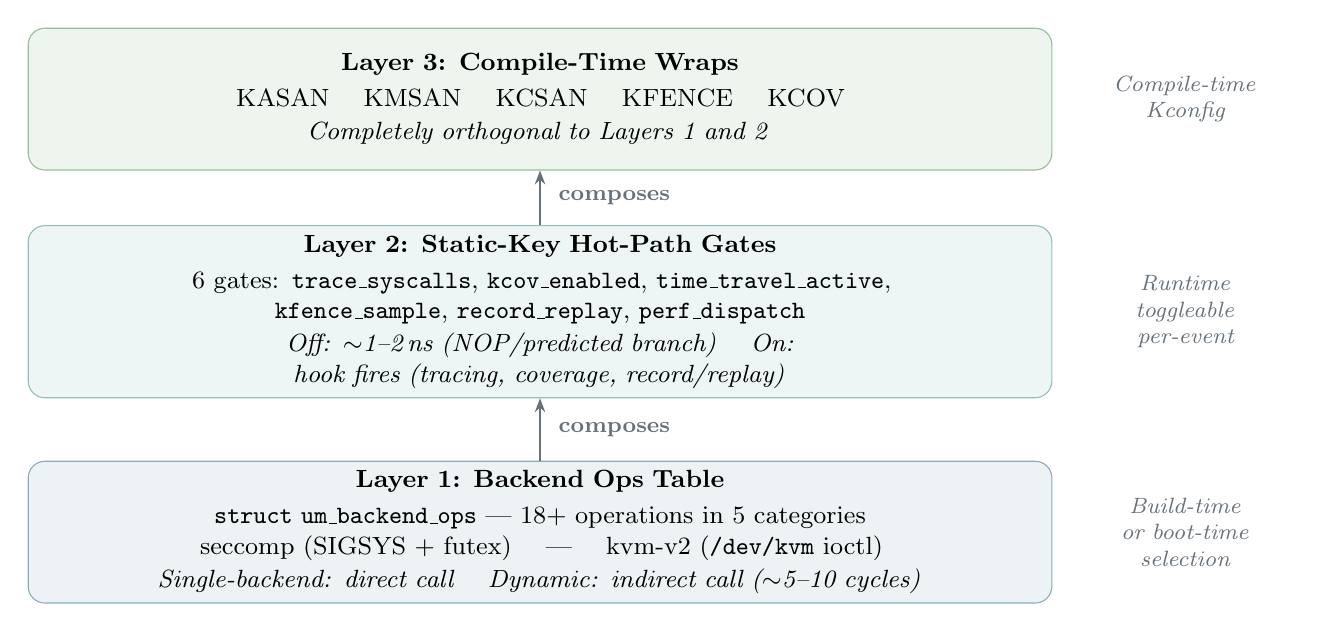
\begin{tikzpicture}[
  layer/.style={
    draw, rounded corners=6pt, minimum width=13cm, minimum height=1.8cm,
    font=\small, align=center, text width=12cm
  },
  arr/.style={-{Stealth[length=5pt]}, thick, color=UMLMuted},
  lbl/.style={font=\footnotesize\bfseries, color=UMLMuted}
]

% Layer 3 — top
\node[layer, fill=UMLGreen!8, draw=UMLGreen!50] (l3) at (0,6.5)
  {\textbf{Layer 3: Compile-Time Wraps}\\[2pt]
   KASAN \quad KMSAN \quad KCSAN \quad KFENCE \quad KCOV\\[1pt]
   \textit{Completely orthogonal to Layers 1 and 2}};

% Layer 2 — middle
\node[layer, fill=UMLTeal!8, draw=UMLTeal!50] (l2) at (0,3.8)
  {\textbf{Layer 2: Static-Key Hot-Path Gates}\\[2pt]
   6 gates: \texttt{trace\_syscalls}, \texttt{kcov\_enabled},
   \texttt{time\_travel\_active},\\
   \texttt{kfence\_sample}, \texttt{record\_replay},
   \texttt{perf\_dispatch}\\[1pt]
   \textit{Off: $\sim$1--2\,ns (NOP/predicted branch) \quad
   On: hook fires (tracing, coverage, record/replay)}};

% Layer 1 — bottom
\node[layer, fill=UMLBlue!8, draw=UMLBlue!50] (l1) at (0,1.0)
  {\textbf{Layer 1: Backend Ops Table}\\[2pt]
   \texttt{struct um\_backend\_ops} --- 18+ operations in 5 categories\\
   seccomp (SIGSYS + futex) \quad | \quad kvm-v2 (\texttt{/dev/kvm} ioctl)\\[1pt]
   \textit{Single-backend: direct call \quad Dynamic: indirect call
   ($\sim$5--10 cycles)}};

% Cost arrows
\draw[arr] (l1.north) -- (l2.south)
  node[midway, right=3pt, lbl] {composes};
\draw[arr] (l2.north) -- (l3.south)
  node[midway, right=3pt, lbl] {composes};

% Side annotation
\node[font=\footnotesize\itshape, color=UMLMuted, text width=3cm, align=center]
  at (8.2,3.8) {Runtime\\toggleable\\per-event};
\node[font=\footnotesize\itshape, color=UMLMuted, text width=3cm, align=center]
  at (8.2,1.0) {Build-time\\or boot-time\\selection};
\node[font=\footnotesize\itshape, color=UMLMuted, text width=3cm, align=center]
  at (8.2,6.5) {Compile-time\\Kconfig};

\end{tikzpicture}
\caption{The three-layer architecture of UML's v2 redesign.  Each layer
  composes orthogonally with the others.}
\label{fig:three-layers}
\end{figure}


\subsection{Layer 1: The Backend Ops Table}
\label{sec:layer1}

The foundation of the architecture is \texttt{struct um\_backend\_ops}, defined
in \texttt{arch/um/include/shared/backend.h}.  Every backend---seccomp,
kvm-v2, and any future backend---populates a single global instance of this
structure.  The structure carries a contract version
(\texttt{UM\_BACKEND\_CONTRACT\_VERSION}, currently~2), a backend kind
enumeration, four capability flags, and 18 function pointers organized into
five categories:

\begin{lstlisting}[language=KernelC, caption={Abbreviated
  \texttt{struct um\_backend\_ops} (from
  \texttt{arch/um/include/shared/backend.h}).},
  label={lst:backend-ops}]
struct um_backend_ops {
    const char       *name;
    enum um_backend_kind kind;
    u32              contract_version;

    /* Capability flags */
    bool  uses_stub_reaper;
    bool  has_syscall_stub_fd_map;
    bool  stub_syscall_uses_futex;
    bool  stub_child_runs_seccomp;

    /* Lifecycle and trap (4) */
    int  (*probe)(void);
    int  (*init)(const struct um_backend_args *args);
    void (*shutdown)(void);
    void (*vcpu_run)(struct uml_pt_regs *regs);         /* HOT */

    /* Memory (5) */
    int  (*mm_create)(struct mm_struct *mm);
    void (*mm_destroy)(struct mm_struct *mm);
    int  (*mm_region_added)(...);                        /* HOT */
    int  (*mm_region_removed)(...);                      /* HOT */
    int  (*mm_region_protected)(...);

    /* Scheduling (4 + 1 optional) */
    int  (*thread_create)(...);
    int  (*thread_start_idle)(...);
    void (*context_switch)(struct task_struct *prev,     /* HOT */
                           struct task_struct *next);
    int  (*ipi_send)(int cpu, int vector);
    void (*tlb_kick_others)(struct mm_struct *mm);  /* may be NULL */

    /* Time (3) */
    u64  (*read_clock_ns)(void);                        /* HOT */
    int  (*set_timer)(int cpu, u64 deadline_ns,
                      enum um_timer_mode mode);
    u64  (*read_persistent_clock_ns)(void);

    /* Debug / introspection (3) */
    void (*init_thread_regs)(...);
    int  (*read_guest_regs)(...);
    int  (*write_guest_regs)(...);
};
\end{lstlisting}

The \textbf{HOT ops}---\texttt{vcpu\_run}, \texttt{mm\_region\_added},
\texttt{mm\_region\_removed}, \texttt{context\_switch}, and
\texttt{read\_clock\_ns}---are the operations invoked on every guest system
call, page fault, context switch, or timer read.  These are validated non-NULL
at boot time by \texttt{validate\_hot\_ops()} in
\umlpath{arch/um/kernel/backend.c}; a NULL hot op triggers an immediate kernel
panic with a diagnostic message identifying the missing operation.

The dispatch macro provides the performance-critical abstraction:

\begin{lstlisting}[language=KernelC, caption={The dispatch macro resolves at
  compile time in single-backend builds.}, label={lst:dispatch-macro}]
#if defined(CONFIG_UM_BACKEND_SECCOMP_ONLY)
# define um_backend_dispatch(op, ...) seccomp_##op(__VA_ARGS__)
#else
# define um_backend_dispatch(op, ...) (um_backend->op(__VA_ARGS__))
#endif
\end{lstlisting}

In a single-backend build (\kconfig{UM\_BACKEND\_SECCOMP\_ONLY}), the macro
expands to a direct function call via token pasting---zero indirect dispatch
overhead.  In a dynamic build (\kconfig{UM\_BACKEND\_DYNAMIC}), the macro
becomes a function pointer dereference through the global
\texttt{um\_backend} pointer, costing a single well-predicted indirect call
($\sim$5--10 cycles on modern x86).


\subsection{Layer 2: Static-Key Hot-Path Gates}
\label{sec:layer2}

Layer~2 addresses a design tension that plagues every kernel instrumentation
system: the choice between \emph{fast} and \emph{observable}.  Traditional
approaches force this choice at compile time (e.g., enabling
\kconfig{FTRACE} imposes a permanent overhead) or at boot time (e.g., kernel
command-line tracing parameters).  UML's static-key gates make observability a
\emph{runtime decision per event}.

The mechanism uses Linux's jump-label infrastructure
(\texttt{<linux/jump\_label.h>}).  Each gate is a
\texttt{DEFINE\_STATIC\_KEY\_FALSE} instance.  When off, the call site contains
either a 5-byte NOP (with \texttt{HAVE\_ARCH\_JUMP\_LABEL}) or a load-compare
branch that the CPU's branch predictor resolves in under 2\,ns.  When on, the
jump-label machinery patches the NOP to a jump into the slow-path handler.

Six gates are currently defined, each controlling a family of hook sites:

\begin{enumerate}[leftmargin=2em, itemsep=2pt]
\item \texttt{um\_hook\_trace\_syscalls} --- system call entry/exit tracing,
  page fault tracing, context switch tracing, IRQ entry tracing, clock read
  tracing.
\item \texttt{um\_hook\_kcov\_enabled} --- coverage-guided fuzzing feedback
  at syscall boundaries.
\item \texttt{um\_hook\_time\_travel\_active} --- deterministic time injection
  for reproducible execution.
\item \texttt{um\_hook\_kfence\_sample} --- KFENCE heap sampling at clock ticks.
\item \texttt{um\_hook\_record\_replay} --- record/replay event capture at
  syscall, page fault, context switch, IRQ, and clock boundaries.
\item \texttt{um\_hook\_perf\_dispatch} --- performance counter dispatch at
  syscall and context switch points.
\end{enumerate}

The hook helpers are declared \texttt{\_\_always\_inline} so that the
static-branch check expands \emph{at the call site}, not inside a function
prologue.  A typical helper composes multiple gates:

\begin{lstlisting}[language=KernelC, caption={The \texttt{um\_on\_syscall\_entry}
  hook helper composes four gates into a single inline expansion.},
  label={lst:hook-helper}]
static __always_inline void um_on_syscall_entry(struct pt_regs *regs)
{
    if (static_branch_unlikely(&um_hook_trace_syscalls))
        __um_trace_syscall_entry(regs);
    if (static_branch_unlikely(&um_hook_kcov_enabled))
        __um_kcov_record_syscall(regs);
    if (static_branch_unlikely(&um_hook_record_replay))
        __um_record_event_syscall_entry(regs);
    if (static_branch_unlikely(&um_hook_perf_dispatch))
        __um_perf_syscall(regs);
}
\end{lstlisting}

Gate state is toggled at runtime through debugfs:
\texttt{/sys/kernel/debug/um/hooks/<name>} accepts writes of \texttt{1} (on)
or \texttt{0} (off).  Each gate maintains per-CPU hit counters, summed
on read through \texttt{um\_hook\_stats\_read()}, for observability without
cross-CPU cacheline contention.

An in-kernel microbenchmark
(\umlpath{arch/um/kernel/hooks\_bench.c}) measures per-gate
cost at runtime via debugfs: 10 batches of 100{,}000 iterations each per hook
site, median reported.  This is the source of truth for the cost model.


\subsection{Layer 3: Compile-Time Wraps}
\label{sec:layer3}

Layer~3 comprises the standard kernel sanitizer and coverage tools that UML
supports by virtue of being a ``normal'' architecture port compiled by a
standard compiler toolchain:

\begin{itemize}[leftmargin=2em, itemsep=2pt]
\item \textbf{KASAN} (Kernel Address Sanitizer)~\cite{kasan} --- detects
  out-of-bounds and use-after-free bugs in slab/page allocator objects.
\item \textbf{KMSAN} (Kernel Memory Sanitizer)~\cite{kmsan} --- detects
  uses of uninitialized memory.
\item \textbf{KCSAN} (Kernel Concurrency Sanitizer)~\cite{kcsan} --- detects
  data races via compile-time instrumentation of memory accesses.
\item \textbf{KFENCE} --- lightweight probabilistic heap-object guard-page
  detection, sampling at timer ticks (gated by the Layer~2
  \texttt{kfence\_sample} hook).
\item \textbf{KCOV} --- coverage-guided fuzzing feedback, collecting per-task
  coverage bitmaps for tools like syzkaller~\cite{syzkaller}.
\end{itemize}

These wraps are completely orthogonal to Layers~1 and~2.  A KASAN-instrumented
UML running the seccomp backend with all Layer~2 gates off is a valid
configuration; so is a clean (no-sanitizer) UML running the kvm-v2 backend with
all gates on.  The three layers multiply rather than interfere.


\subsection{Cost Model}
\label{sec:cost-model}

Table~\ref{tab:cost-model} shows the approximate per-event overhead for each
layer and their composition into representative profiles.  The baseline is a
``bare'' guest system call round-trip (guest $\to$ trap $\to$ kernel
$\to$ return).  All figures assume x86-64, seccomp backend, single-backend
inline dispatch.

\begin{table}[ht]
\centering
\caption{Per-syscall-roundtrip cost model across layers and profiles.
  Figures are representative; actual measurements vary with host
  microarchitecture and workload.}
\label{tab:cost-model}
\rowcolors{2}{UMLPanel}{white}
\begin{tabular}{l r r r r}
\toprule
\textbf{Profile} & \textbf{Layer 1} & \textbf{Layer 2} & \textbf{Layer 3}
  & \textbf{Total overhead} \\
\midrule
\texttt{prod-fast}
  & 0 (inline)     & $\sim$4--8\,ns (4 NOPs)   & 0           & $\sim$4--8\,ns \\
\texttt{prod-with-hooks}
  & 0 (inline)     & $\sim$50--100\,ns (gates on) & 0         & $\sim$50--100\,ns \\
\texttt{research}
  & $\sim$5--10\,ns & $\sim$50--100\,ns        & 0           & $\sim$55--110\,ns \\
\texttt{fuzz}
  & 0 (inline)     & $\sim$20--40\,ns (kcov on) & KASAN: 2--3$\times$ & 2--3$\times$ \\
\texttt{fuzz-deep}
  & 0 (inline)     & $\sim$50--100\,ns          & KASAN+KMSAN: 4--6$\times$ & 4--6$\times$ \\
\texttt{race}
  & $\sim$5--10\,ns & $\sim$50--100\,ns        & KCSAN: 3--5$\times$ & 3--5$\times$ \\
\bottomrule
\end{tabular}
\end{table}

The key insight is that Layers~1 and~2 add \emph{nanoseconds} of overhead per
event, while Layer~3 (sanitizers) dominates total cost when enabled.  The
three-layer decomposition ensures that the fast path pays only for what it
uses, and the decision to enable observability never requires a rebuild.


% --------------------------------------------------------------------------
\section{Backend Selection Mechanism}
\label{sec:backend-selection}

Backend selection operates at two levels: \emph{build-time} configuration
through Kconfig, and \emph{boot-time} resolution through the
\texttt{backend=} kernel command-line parameter.

\subsection{Build-Time: Kconfig}

The Kconfig choice block in \umlpath{arch/um/Kconfig} offers two dispatch
modes:

\begin{description}[leftmargin=2em, style=nextline]
\item[\kconfig{UM\_BACKEND\_SECCOMP\_ONLY}]
  Single-backend inline dispatch.  The \texttt{um\_backend\_dispatch()} macro
  expands to direct \texttt{seccomp\_<op>()} calls via token pasting.  Zero
  indirect-dispatch cost.  Smallest binary.  This is the recommended mode for
  production and sandbox deployments.

\item[\kconfig{UM\_BACKEND\_DYNAMIC}]
  Multi-backend indirect dispatch.  Compiles every available backend
  (currently seccomp; kvm-v2 joins this path once its Phase~A integration
  is complete).  The dispatch macro dereferences the global
  \texttt{um\_backend} pointer, costing one well-predicted indirect call per
  site.  This is the recommended mode for distribution kernels and CI matrices
  that need a single binary to support multiple backends.
\end{description}

Both modes \texttt{select UM\_BACKEND\_SECCOMP}; the seccomp backend is always
available.  The kvm-v2 backend is gated by \kconfig{UM\_BACKEND\_KVM\_V2},
which in turn depends on \texttt{EXPERT} and \kconfig{UM\_BACKEND\_DYNAMIC}.

\begin{figure}[ht]
\centering
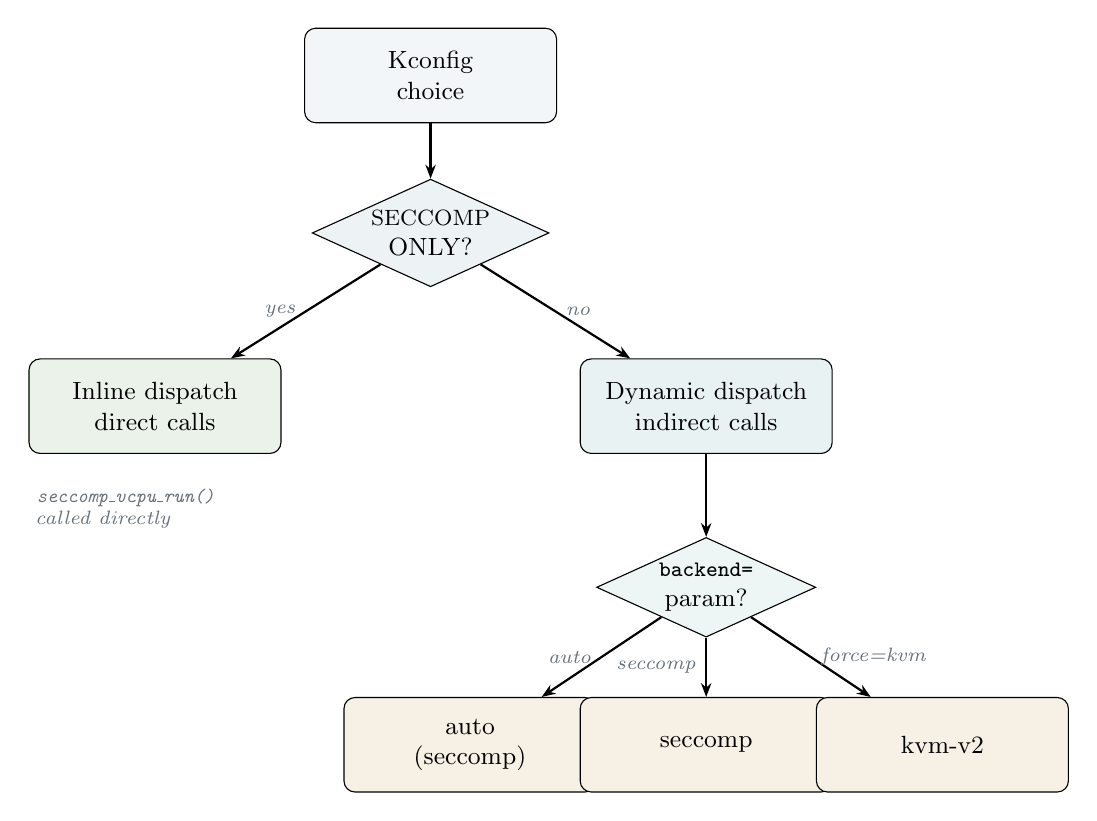
\begin{tikzpicture}[
  box/.style={draw, rounded corners=4pt, minimum width=3.2cm,
              minimum height=1.2cm, font=\small, align=center},
  decision/.style={draw, diamond, aspect=2.2, inner sep=1pt,
                   font=\small, align=center},
  arr/.style={-{Stealth[length=5pt]}, thick},
  note/.style={font=\scriptsize\itshape, color=UMLMuted}
]

\node[box, fill=UMLPanel] (start) at (0,0) {Kconfig\\choice};

\node[decision, fill=UMLBlue!8] (kc) at (0,-2)
  {\footnotesize SECCOMP\\ONLY?};

\node[box, fill=UMLGreen!10] (inline) at (-3.5,-4.2)
  {Inline dispatch\\direct calls};
\node[box, fill=UMLTeal!10] (dyn) at (3.5,-4.2)
  {Dynamic dispatch\\indirect calls};

\node[decision, fill=UMLTeal!8] (boot) at (3.5,-6.5)
  {\footnotesize \texttt{backend=}\\param?};

\node[box, fill=UMLAmber!10] (auto) at (0.5,-8.5) {auto\\(seccomp)};
\node[box, fill=UMLAmber!10] (seccomp) at (3.5,-8.5) {seccomp};
\node[box, fill=UMLAmber!10] (kvm) at (6.5,-8.5) {kvm-v2};

\draw[arr] (start) -- (kc);
\draw[arr] (kc) -- node[left, note] {yes} (inline);
\draw[arr] (kc) -- node[right, note] {no} (dyn);
\draw[arr] (dyn) -- (boot);
\draw[arr] (boot) -- node[left, note] {auto} (auto);
\draw[arr] (boot) -- node[left, note] {seccomp} (seccomp);
\draw[arr] (boot) -- node[right, note] {force=kvm} (kvm);

\node[note, text width=3cm] at (-3.5,-5.5)
  {\texttt{seccomp\_vcpu\_run()}\\called directly};

\end{tikzpicture}
\caption{Backend selection flow: build-time Kconfig choice followed by
  boot-time parameter resolution.}
\label{fig:backend-selection}
\end{figure}


\subsection{Boot-Time: \texttt{init\_backend()}}

The function \texttt{init\_backend()} in \umlpath{arch/um/kernel/backend.c} is
called once from \texttt{setup\_arch()} during early boot.  It resolves the
backend selection, validates HOT ops, invokes the backend's \texttt{probe()}
and \texttt{init()} lifecycle ops, and sets the immutable global
\texttt{um\_backend} pointer.

In \kconfig{UM\_BACKEND\_DYNAMIC} builds, the resolution cascade in
\texttt{pick\_dynamic\_backend()} is:

\begin{enumerate}[leftmargin=2em]
\item If \texttt{backend=force=<kind>} was specified and the requested backend
  is not compiled in, the kernel panics immediately.
\item If \texttt{backend=<kind>} was specified (non-force), the requested
  backend is used if available; otherwise the kernel falls back with a
  \texttt{pr\_warn}.
\item If \texttt{backend=auto} (the default) or no parameter was given, the
  seccomp backend is selected.
\end{enumerate}

The ptrace backend was removed entirely in the v2 refactoring.  Requesting
\texttt{backend=force=ptrace} triggers a panic with a diagnostic message
directing the user to pin to v6.16 or earlier.


% --------------------------------------------------------------------------
\section{The Stub Mechanism}
\label{sec:stub-mechanism}

The seccomp backend's core abstraction is the \emph{stub child}: a minimal
host process that serves as the execution container for a single guest
\texttt{mm\_struct}.  Each guest address space gets its own stub child, created
by \texttt{mm\_create()} and destroyed by \texttt{mm\_destroy()}.  The stub
provides the host-side process context in which guest userspace code runs
and guest system calls are intercepted.

\subsection{Stub Lifecycle}

When a new guest \texttt{mm\_struct} is created (e.g., on \texttt{fork()} or
\texttt{exec()}), the seccomp backend's \texttt{mm\_create} op clones a new
host child process.  This child---the stub---is not a conventional process.  It
executes a minimal trampoline (the ``stub code'') that:

\begin{enumerate}[leftmargin=2em]
\item Installs a seccomp BPF filter~\cite{seccomp-bpf} that traps all system
  calls, delivering \texttt{SIGSYS} to the stub's signal handler instead of
  executing the syscall on the host.
\item Maps a shared communication page (the \texttt{stub\_data} structure) at a
  fixed address in its address space.
\item Enters an infinite loop: wait on a futex in \texttt{stub\_data},
  process a batch of memory-management syscalls, and signal completion.
\end{enumerate}

\subsection{The \texttt{stub\_data} Structure}

The shared \texttt{stub\_data} page (Listing~\ref{lst:stub-data}) is the
communication channel between the UML kernel (running in the host parent
process) and the stub child.  It occupies exactly one page
(\texttt{UM\_KERN\_PAGE\_SIZE}) and contains:

\begin{lstlisting}[language=KernelC, caption={The \texttt{stub\_data}
  structure (from \texttt{arch/um/include/shared/skas/stub-data.h}).},
  label={lst:stub-data}]
struct stub_data {
    long err;
    int syscall_data_len;
    struct stub_syscall syscall_data[...] __aligned(16);

    /* Shared with signal handler (seccomp mode) */
    short restart_wait;
    unsigned int futex;   /* FUTEX_IN_CHILD or FUTEX_IN_KERN */
    int signal;
    unsigned short si_offset;
    unsigned short mctx_offset;

    struct stub_data_arch arch_data;

    /* Signal handler stack */
    unsigned char sigstack[UM_KERN_PAGE_SIZE]
        __aligned(UM_KERN_PAGE_SIZE);
};
\end{lstlisting}

The \texttt{syscall\_data} array holds a batch of \texttt{mmap}/\texttt{munmap}
operations that the stub executes on behalf of the UML kernel's TLB
synchronization layer.  Batching amortizes the futex wake/wait round-trip cost
across multiple memory operations.

\subsection{Futex-Based Synchronization}

\begin{figure}[ht]
\centering
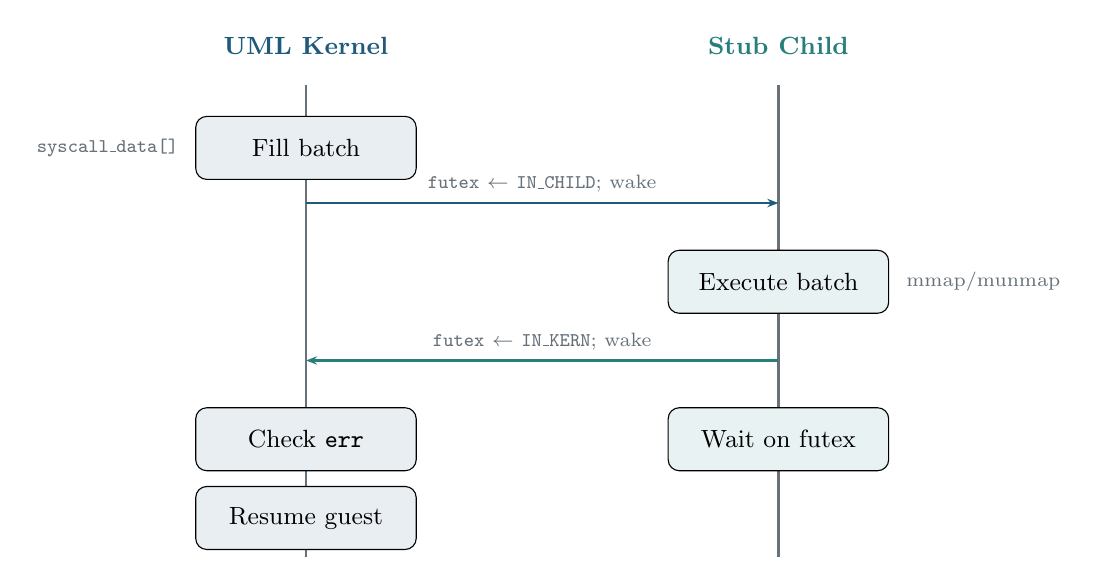
\begin{tikzpicture}[
  proc/.style={draw, rounded corners=4pt, minimum width=2.8cm,
               minimum height=0.8cm, font=\small, fill=#1},
  msg/.style={-{Stealth[length=4pt]}, thick, color=#1},
  note/.style={font=\scriptsize, color=UMLMuted},
  timeline/.style={thick, color=UMLMuted}
]

% UML kernel (parent) timeline
\node[font=\small\bfseries, color=UMLBlue] at (-3,5.5) {UML Kernel};
\draw[timeline] (-3,5) -- (-3,-1);

% Stub child timeline
\node[font=\small\bfseries, color=UMLTeal] at (3,5.5) {Stub Child};
\draw[timeline] (3,5) -- (3,-1);

% Step 1: Kernel fills syscall batch
\node[proc=UMLBlue!10] (k1) at (-3,4.2) {Fill batch};
\node[note, anchor=east] at (-4.5,4.2) {\texttt{syscall\_data[]}};

% Step 2: futex = FUTEX_IN_CHILD, wake
\draw[msg=UMLBlue] (-3,3.5) -- node[above, note]
  {\texttt{futex} $\leftarrow$ \texttt{IN\_CHILD}; wake} (3,3.5);

% Step 3: Stub processes batch
\node[proc=UMLTeal!10] (s1) at (3,2.5) {Execute batch};
\node[note, anchor=west] at (4.5,2.5) {mmap/munmap};

% Step 4: futex = FUTEX_IN_KERN, wake parent
\draw[msg=UMLTeal] (3,1.5) -- node[above, note]
  {\texttt{futex} $\leftarrow$ \texttt{IN\_KERN}; wake} (-3,1.5);

% Step 5: Kernel reads err
\node[proc=UMLBlue!10] (k2) at (-3,0.5) {Check \texttt{err}};

% Step 6: Resume guest
\node[proc=UMLBlue!10] (k3) at (-3,-0.5) {Resume guest};
\node[proc=UMLTeal!10] (s2) at (3,0.5) {Wait on futex};

\end{tikzpicture}
\caption{Futex-based synchronization between the UML kernel and the seccomp
  stub child.  The shared \texttt{stub\_data.futex} field alternates between
  \texttt{FUTEX\_IN\_CHILD} and \texttt{FUTEX\_IN\_KERN}.}
\label{fig:stub-sync}
\end{figure}

Communication uses a single \texttt{unsigned int futex} field in
\texttt{stub\_data}.  The protocol is simple
(Figure~\ref{fig:stub-sync}):

\begin{enumerate}[leftmargin=2em]
\item The UML kernel fills the \texttt{syscall\_data} array with the batch of
  memory operations to perform.
\item The kernel sets \texttt{futex = FUTEX\_IN\_CHILD} and issues a
  \texttt{FUTEX\_WAKE} system call~\cite{futex-lwn}.
\item The stub child wakes, iterates through \texttt{syscall\_data}, executes
  each mmap/munmap, and records any error in \texttt{err}.
\item The stub sets \texttt{futex = FUTEX\_IN\_KERN} and issues
  \texttt{FUTEX\_WAKE}.
\item The kernel wakes, checks \texttt{err}, and proceeds.
\end{enumerate}

This is substantially faster than the old ptrace-based mechanism, which
required a \texttt{PTRACE\_SETREGS} + \texttt{PTRACE\_CONT} + wait round-trip
per operation~\cite{ptrace-man}.  The seccomp path achieves roughly 3--4$\times$
lower syscall round-trip latency.


% --------------------------------------------------------------------------
\section{Guest Memory Management}
\label{sec:guest-mm}

UML's guest physical memory is backed by a host-side memory object: typically
an anonymous \texttt{mmap} or a \texttt{tmpfs} file.  Guest page table changes
are not self-effectuating---there is no hardware MMU to walk guest page tables.
Instead, every guest PTE modification must be translated into a host system
call (\texttt{mmap}, \texttt{munmap}, or \texttt{mprotect}) that adjusts the
stub child's host address space to match.

\subsection{The TLB Synchronization Layer}

The mm-arbiter in \umlpath{arch/um/kernel/tlb.c} implements the
\texttt{um\_tlb\_sync()} function, which is the single drain point for pending
guest page table changes.  The flow is:

\begin{enumerate}[leftmargin=2em]
\item Guest kernel code (e.g., \texttt{do\_mmap}, \texttt{do\_munmap},
  page fault handler) modifies PTEs and calls \texttt{um\_tlb\_mark\_sync()},
  which records the affected address range in per-mm
  \texttt{sync\_tlb\_range\_from}/\texttt{sync\_tlb\_range\_to} fields.
\item Before the next guest userspace entry (\texttt{vcpu\_run}),
  \texttt{um\_tlb\_sync()} walks the per-mm page table over the marked range,
  inspects \texttt{pte\_needsync()} on each leaf, and emits a
  \texttt{struct um\_memory\_region} per dirty PTE.
\item Each region is dispatched through the backend's
  \texttt{mm\_region\_added()} or \texttt{mm\_region\_removed()} op.  For the
  seccomp backend, these ops translate into stub child mmap/munmap batches.
  For kvm-v2, they translate into KVM memslot updates.
\item After a successful drain, the mm-arbiter increments the per-mm
  \texttt{tlb\_gen} counter and, if the backend provides a
  \texttt{tlb\_kick\_others} op, invokes it to notify other vCPUs.
\end{enumerate}

\subsection{SMP TLB Generation Tracking}
\label{sec:tlb-gen}

Under SMP, multiple vCPUs may be executing code from the same
\texttt{mm\_struct} concurrently.  When one vCPU modifies a page table and
drains via \texttt{um\_tlb\_sync()}, the other vCPUs must be notified so they
can flush their local view of the guest TLB.

The mechanism uses two counters per mm, defined in
\umlpath{arch/um/include/asm/mmu.h}:

\begin{lstlisting}[language=KernelC, caption={Per-mm TLB generation counters
  for SMP coherence.}, label={lst:tlb-gen}]
typedef struct mm_context {
    /* ... */
    atomic64_t tlb_gen;
    atomic64_t tlb_gen_seen_by[NR_CPUS];
} mm_context_t;
\end{lstlisting}

\begin{itemize}[leftmargin=2em]
\item \texttt{tlb\_gen}: a monotonically increasing counter, incremented after
  each successful \texttt{um\_tlb\_sync()} drain.
\item \texttt{tlb\_gen\_seen\_by[cpu]}: for each vCPU, the most recent
  \texttt{tlb\_gen} value at which that vCPU flushed its local TLB state.
\end{itemize}

On each \texttt{vcpu\_run} dispatch, the vCPU compares its
\texttt{tlb\_gen\_seen\_by[cpu]} against the current \texttt{tlb\_gen}.  On
mismatch, it performs a guest TLB flush (for kvm-v2, a CR4.PGE toggle inside
KVM\_RUN) and updates its slot.

The cross-vCPU kick is targeted: \texttt{tlb\_kick\_others()} only sends IPIs
to vCPUs whose \texttt{tlb\_gen\_seen\_by[cpu]} is stale relative to the
current mm's \texttt{tlb\_gen}.  This narrowing eliminates the IPI storm that a
broadcast approach would cause under high mm-churn workloads.

An important subtlety: \texttt{tlb\_gen\_seen\_by} is per-(mm, cpu), not
per-vCPU globally.  A previous design used a single per-vCPU
\texttt{last\_seen\_tlb\_gen} counter, but this suffered from cross-mm
contamination: dispatching mm$_B$ (gen=5) after mm$_A$ (gen=3000) wrote 5 into
the single counter, causing a return to mm$_A$ to see a spurious lag of 2995
and potentially misleading the kicker.

\subsection{Deferred Free: The mmu\_gather Integration}

A subtlety of UML's deferred TLB-sync model is that it violates the standard
\texttt{mmu\_gather} contract.  In a hardware architecture, \texttt{mmu\_gather}
collects pages during an unmap, issues a TLB flush, and then frees the pages.
In UML, the TLB flush does not happen until the next \texttt{vcpu\_run}
dispatch.  This creates a window where freed pages could be reused by the
kernel while stale TLB entries still point to them.

The fix (rooted in \texttt{mm\_context\_t.deferred\_free\_pages}) intercepts
the page-free path: instead of releasing pages immediately, they are queued
on a per-mm deferred list and freed at the start of the next
\texttt{vcpu\_run}, after the guest TLB has been flushed.


% --------------------------------------------------------------------------
\section{SMP Implementation}
\label{sec:smp}

UML implements symmetric multiprocessing by running one host pthread per
virtual CPU.  This is a cooperative model: the host kernel schedules the
pthreads, and UML's scheduler runs within each pthread to multiplex guest
tasks.

\subsection{Thread Model}

\begin{figure}[ht]
\centering
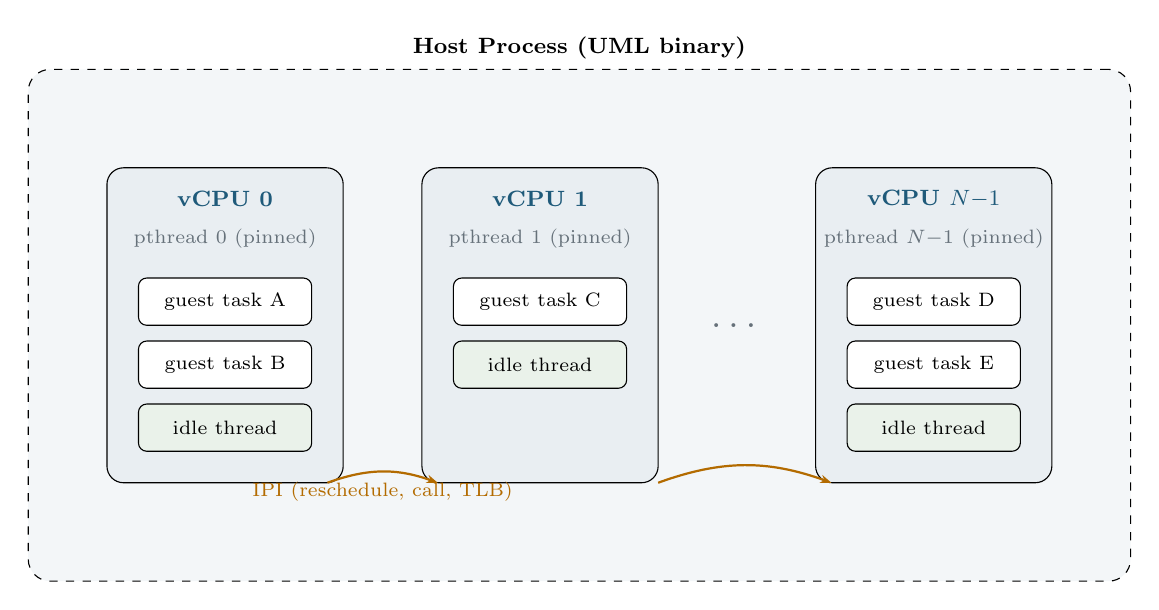
\begin{tikzpicture}[
  cpu/.style={draw, rounded corners=6pt, minimum width=3cm,
              minimum height=4cm, fill=#1, font=\small},
  task/.style={draw, rounded corners=3pt, minimum width=2.2cm,
               minimum height=0.6cm, fill=white, font=\scriptsize},
  arr/.style={-{Stealth[length=4pt]}, thick, color=UMLMuted},
  lbl/.style={font=\footnotesize\bfseries}
]

% Host process box
\node[draw, dashed, rounded corners=8pt, minimum width=14cm,
      minimum height=6.5cm, fill=UMLPanel, label={[lbl]above:Host Process
      (UML binary)}] at (0,0) {};

% vCPU 0
\node[cpu=UMLBlue!10] (cpu0) at (-4.5,0) {};
\node[lbl, color=UMLBlue] at (-4.5,1.6) {vCPU 0};
\node[font=\scriptsize, color=UMLMuted] at (-4.5,1.1)
  {pthread 0 (pinned)};
\node[task] at (-4.5,0.3) {guest task A};
\node[task] at (-4.5,-0.5) {guest task B};
\node[task, fill=UMLGreen!10] at (-4.5,-1.3) {idle thread};

% vCPU 1
\node[cpu=UMLBlue!10] (cpu1) at (-0.5,0) {};
\node[lbl, color=UMLBlue] at (-0.5,1.6) {vCPU 1};
\node[font=\scriptsize, color=UMLMuted] at (-0.5,1.1)
  {pthread 1 (pinned)};
\node[task] at (-0.5,0.3) {guest task C};
\node[task, fill=UMLGreen!10] at (-0.5,-0.5) {idle thread};

% vCPU N-1
\node[cpu=UMLBlue!10] (cpuN) at (4.5,0) {};
\node[lbl, color=UMLBlue] at (4.5,1.6) {vCPU $N{-}1$};
\node[font=\scriptsize, color=UMLMuted] at (4.5,1.1)
  {pthread $N{-}1$ (pinned)};
\node[task] at (4.5,0.3) {guest task D};
\node[task] at (4.5,-0.5) {guest task E};
\node[task, fill=UMLGreen!10] at (4.5,-1.3) {idle thread};

% Dots
\node[font=\Large, color=UMLMuted] at (2,0) {\ldots};

% IPI arrows
\draw[arr, color=UMLAmber, bend left=20] (-3.2,-2) to
  node[below, font=\scriptsize, color=UMLAmber] {IPI (reschedule, call, TLB)}
  (-1.8,-2);
\draw[arr, color=UMLAmber, bend left=20] (1,-2) to (3.2,-2);

\end{tikzpicture}
\caption{UML SMP thread model: one host pthread per virtual CPU, each pinned
  to a host CPU via \texttt{pthread\_setaffinity\_np}.  Guest tasks are
  scheduled within each pthread by UML's copy of the Linux scheduler.}
\label{fig:smp-model}
\end{figure}

At boot time, CPU~0 runs on the main thread.  For each additional CPU
($1$ through $N{-}1$), \texttt{os\_start\_cpu\_thread()} in
\umlpath{arch/um/os-Linux/smp.c} calls \texttt{pthread\_create()} to spawn a
new host thread.  Each thread is immediately pinned to the corresponding host
CPU via \texttt{pthread\_setaffinity\_np()} (SMP-T37):

\begin{lstlisting}[language=KernelC, caption={CPU affinity pinning for vCPU
  threads (from \texttt{arch/um/os-Linux/smp.c}).}, label={lst:affinity}]
cpu_set_t cpuset;
CPU_ZERO(&cpuset);
CPU_SET(cpu, &cpuset);
pthread_setaffinity_np(cpu_threads[cpu], sizeof(cpuset), &cpuset);
\end{lstlisting}

This pinning ensures that each guest CPU's host thread always executes on the
same physical CPU, which is critical for the kvm-v2 backend's per-host-CPU
vCPU pool: a given guest CPU always dispatches against the same KVM vCPU file
descriptor.

\subsection{Context Switching}

A guest context switch is a call to the backend's \texttt{context\_switch(prev,
next)} op.  For the seccomp backend, this involves saving and restoring the
register state of the stub child process.  For kvm-v2, it involves saving
FPU state from the per-CPU vCPU into \texttt{prev->thread} and loading
\texttt{next->thread}'s saved state.

\subsection{IPI Delivery}

Inter-processor interrupts are sent through \texttt{um\_backend\_dispatch(ipi\_send, cpu, vector)}.  Four IPI vectors are defined:

\begin{description}[leftmargin=2em, font=\ttfamily, itemsep=2pt]
\item[UML\_IPI\_RES] Reschedule request (triggers \texttt{scheduler\_ipi()}).
\item[UML\_IPI\_CALL\_SINGLE] Single-function call
  (\texttt{generic\_smp\_call\_function\_single\_interrupt()}).
\item[UML\_IPI\_CALL] Broadcast function call
  (\texttt{generic\_smp\_call\_function\_interrupt()}).
\item[UML\_IPI\_STOP] CPU offline (enter infinite pause loop).
\end{description}

The template-pause mechanism (\umlpath{arch/um/kernel/template\_pause.c})
builds on top of the IPI infrastructure: it allows the UML kernel to quiesce
all vCPUs to a named ``ready point,'' \texttt{SIGSTOP} the host process for
an external supervisor to fork, and resume with per-child identity blobs.
This is the foundation of the pool-based deployment model.

\subsection{The \texttt{migrate\_disable} Fix (SMP-T13)}
\label{sec:smp-t13}

A critical correctness bug in the kvm-v2 backend's SMP support was discovered
and fixed in the SMP-T13 work item (May~2026).  The issue: UML builds with
\kconfig{PREEMPT\_VOLUNTARY}, which makes \texttt{preempt\_disable()} a no-op.
The kvm-v2 backend's \texttt{vcpu\_run} looks up the per-host-CPU vCPU pointer
using \texttt{smp\_processor\_id()} and then enters \texttt{KVM\_RUN}.  If the
host scheduler migrates the pthread to a different host CPU between the
lookup and the ioctl, the dispatch proceeds against the wrong vCPU---writing
register state to the wrong \texttt{kvm\_run} mmap, executing the wrong
vCPU's code.

The fix uses \texttt{migrate\_disable()}, which pins the running task to its
current host CPU regardless of the preempt-count semantics.  Voluntary
scheduling (e.g., inside \texttt{handle\_syscall} via \texttt{sched\_yield})
is still allowed---the key invariant is that when the task \emph{resumes}, it
resumes on the \emph{same} CPU, so the per-CPU vCPU pointer remains valid.


% --------------------------------------------------------------------------
\section{Device Model}
\label{sec:device-model}

UML provides a set of paravirtualized devices that bridge the guest kernel's
standard driver interfaces to host resources.  These are not emulations of
physical hardware; they are purpose-built drivers that use host system calls
for I/O.

\begin{table}[ht]
\centering
\caption{UML device drivers and their host-side backing mechanisms.}
\label{tab:devices}
\rowcolors{2}{UMLPanel}{white}
\begin{tabularx}{\textwidth}{l l Y}
\toprule
\textbf{Device} & \textbf{Source} & \textbf{Description} \\
\midrule
\texttt{ubd} &
  \texttt{ubd\_kern.c} &
  Block device backed by host files (typically raw disk images or sparse
  files).  Supports multiple partitions, copy-on-write layers, and synchronous
  or asynchronous I/O modes. \\

Vector network &
  \texttt{vector\_kern.c} &
  Legacy network driver using vector (scatter-gather) transport.  Supports
  TAP, raw sockets, and various encapsulation modes. \\

Vector2 network &
  \texttt{vector2\_core.c} &
  Next-generation network driver with a modular transport/model/queue
  architecture.  Supports TAP devices, host file descriptors, ethtool
  statistics, and pluggable queue management.  Default in the v2
  redesign. \\

Console/TTY &
  \texttt{stdio\_console.c} &
  Serial-like consoles mapped to host stdio, PTYs, or named pipes.  Multiple
  virtual consoles supported (\texttt{con0}, \texttt{con1}, \ldots),
  including the stderr console for early-boot diagnostics. \\

\texttt{mconsole} &
  \texttt{mconsole\_kern.c} &
  UML-specific management console accessible via a Unix domain socket.
  Supports runtime commands: \texttt{halt}, \texttt{reboot}, \texttt{config}
  (hot-add devices), \texttt{sysrq}, \texttt{cad} (Ctrl-Alt-Del), and
  \texttt{proc} (read /proc entries from outside). \\

\texttt{virtio-uml} &
  \texttt{virtio\_uml.c} &
  Standard virtio devices using vhost-user sockets.  Allows UML to use the
  same virtio device backends (e.g., vhost-user-blk, vhost-user-net) that
  QEMU and other VMMs use. \\

\texttt{hostfs} &
  \texttt{fs/hostfs/} &
  Passthrough filesystem that maps a host directory tree directly into the
  guest's VFS namespace.  Not a block device driver but a filesystem type
  (\texttt{mount -t hostfs}).  Invaluable for development: edit files on
  the host, see them immediately inside the guest. \\

\texttt{vfio-uml} &
  \texttt{vfio\_kern.c} &
  VFIO device passthrough for assigning host PCI devices to the UML guest
  (requires IOMMU support on the host). \\

Harddog &
  \texttt{harddog\_kern.c} &
  Software watchdog timer backed by a host helper process. \\

RTC &
  \texttt{rtc\_kern.c} &
  Real-time clock providing time-of-day to the guest, backed by host
  \texttt{clock\_gettime}. \\

Random &
  \texttt{random.c} &
  Entropy source backed by host \texttt{/dev/urandom}. \\
\bottomrule
\end{tabularx}
\end{table}

The device model is deliberately thin.  Because UML runs as a userspace process,
it cannot intercept hardware interrupts or DMA transactions.  Instead, UML
devices use file descriptor-based I/O and signal-driven notification
(typically \texttt{SIGIO}) to simulate device interrupts.  The
\umlpath{arch/um/kernel/sigio.c} and \umlpath{arch/um/os-Linux/sigio.c} files
manage the translation of host fd readability events into UML interrupt
delivery.

The vector2 network driver deserves special mention: it replaces the legacy
vector driver with a cleanly layered architecture separating the transport
mechanism (how packets reach the host), the device model (how the kernel sees
the NIC), and the queue management (how packets are buffered and batched).
Each layer is independently testable via KUnit, and the transport layer is
pluggable---adding a new transport (e.g., AF\_XDP) requires implementing a
small interface without touching the core driver.


% --------------------------------------------------------------------------
\section{Build System}
\label{sec:build-system}

Building UML requires specifying \texttt{ARCH=um} on the make command line.
This selects the \umlpath{arch/um/} directory as the architecture-specific
source tree and uses the host's native compiler (no cross-compilation toolchain
needed, since the ``target'' is the host architecture itself running in
userspace).

\subsection{Basic Build}

\begin{lstlisting}[language=bash, caption={Standard UML build commands.},
  label={lst:build}]
# Configure
make ARCH=um O=build/um x86_64_defconfig

# Optional: customize
make ARCH=um O=build/um menuconfig

# Build
make ARCH=um O=build/um -j$(nproc)

# Result: build/um/vmlinux (an ELF binary)
\end{lstlisting}

The output is a standard ELF binary named \texttt{vmlinux} that can be executed
directly from the command line:

\begin{lstlisting}[language=bash]
./build/um/vmlinux mem=512M rootfstype=hostfs \
    rw init=/bin/bash
\end{lstlisting}

\subsection{The \texttt{O=} Discipline}

An important operational requirement is to \emph{always} use the \texttt{O=}
out-of-tree build directory.  A bare \texttt{make ARCH=um} (without \texttt{O=})
contaminates the source tree with generated files that opaquely break future
\texttt{O=} builds.  Recovery requires \texttt{make mrproper} (which removes
all generated files, including \texttt{.config}).  All examples in this report
and in the project's CI configurations use the \texttt{O=build/um} convention.

\subsection{Kconfig Structure}

UML's Kconfig inherits from the host architecture (\texttt{x86} on x86-64
hosts) but adds UML-specific options under the \texttt{UML}-prefixed namespace.
Key configuration groups include:

\begin{description}[leftmargin=2em, style=nextline]
\item[\kconfig{UM\_BACKEND\_*}] Backend selection (Section~\ref{sec:backend-selection}).
\item[\kconfig{UM\_BACKEND\_KVM\_V2}] The v2 KVM backend (requires \texttt{EXPERT}).
\item[\kconfig{UM\_WORKER\_PROCESS}] Per-mm host worker process model.
\item[\kconfig{UM\_TEMPLATE\_PAUSE\_FORK}] Fork-on-resume pool model.
\item[\kconfig{UML\_NET\_*}] Network transport selection (TAP, raw, etc.).
\item[\kconfig{BLK\_DEV\_UBD}] The \texttt{ubd} block device.
\item[\kconfig{HOSTFS}] Host filesystem passthrough.
\end{description}

The \texttt{profiles/} subdirectory under \umlpath{arch/um/configs/} provides
ready-made configurations for common use cases: \texttt{prod-fast} (minimal
overhead, single-backend inline dispatch, no sanitizers),
\texttt{fuzz} (KASAN + KCOV + snapshot/forkserver), \texttt{research}
(dynamic dispatch with all hooks available), and others.

\subsection{SUBARCH and Host Architecture}

UML's build system uses a \texttt{SUBARCH} variable to determine the host
architecture.  On x86-64 systems, \texttt{SUBARCH=x86} is detected
automatically.  The host architecture's headers (e.g., register layouts,
calling conventions, signal frame structures) are pulled in from
\texttt{arch/x86/} via the \texttt{HEADER\_ARCH} mechanism in the top-level
\umlpath{arch/um/Makefile}:

\begin{lstlisting}[language=make, caption={Host architecture header
  selection.}]
HEADER_ARCH := $(SUBARCH)
ifneq ($(filter $(SUBARCH),x86 x86_64 i386),)
    HEADER_ARCH := x86
endif
HOST_DIR := arch/$(HEADER_ARCH)
\end{lstlisting}

This dual-architecture nature---\texttt{arch/um/} for UML-specific code,
\texttt{arch/x86/} for host-specific data structures---is what allows UML to
run unmodified x86-64 binaries in the guest while itself being a fundamentally
different ``architecture'' from the kernel's perspective.


% --------------------------------------------------------------------------
\section{Chapter Summary}
\label{sec:arch-summary}

UML's architecture is the product of a sustained negotiation between the
abstractions the Linux kernel expects from a hardware platform and the
mechanisms available through the host kernel's system call interface.  The v2
redesign formalized this negotiation into three orthogonal layers:

\begin{enumerate}[leftmargin=2em]
\item A \textbf{backend ops table} that encapsulates the trap mechanism behind
  a stable 18-operation interface, enabling both seccomp and KVM backends to
  coexist with zero code duplication in the shared kernel paths.
\item \textbf{Static-key gates} that make observability a per-event runtime
  decision, with nanosecond-scale overhead when disabled and no rebuild
  required to toggle.
\item \textbf{Compile-time sanitizer wraps} that compose with the first two
  layers without interference, enabling the full spectrum from bare-metal-speed
  production to deep sanitizer coverage.
\end{enumerate}

The stub mechanism, TLB generation tracking, SMP thread pinning, and device
model complete the picture of a virtual machine monitor that is simultaneously
a kernel architecture port, a testing platform, and a research vehicle.
Chapter~\ref{ch:implementation} explores the implementation details of each
subsystem, and Chapter~\ref{ch:kvm} describes how the kvm-v2 backend
leverages this architecture to add hardware-accelerated execution.

% ==========================================================================
%  Chapter 5 — UML Implementation Details
% ==========================================================================
\chapter{UML Implementation Details}
\label{ch:implementation}

\epigraph{%
  Show me the data structures and I won't usually need your code;
  it will be obvious.%
}{Fred Brooks, paraphrased}

This chapter descends from the architectural overview of the previous chapters
into the concrete data structures, code paths, and protocols that make
User-Mode Linux work.  Where earlier chapters described \emph{what} UML does,
this chapter describes \emph{how}: the exact sequence of system calls, signal
deliveries, futex operations, and page-table walks that execute when a guest
process issues a system call, takes a page fault, or is context-switched.
All code references are relative to the \texttt{arch/um/} subtree of the Linux
6.16+ source unless noted otherwise.

% ------------------------------------------------------------------
\section{Process Lifecycle}
\label{sec:impl-process-lifecycle}

A UML guest process is, from the host kernel's perspective, just another
userspace thread.  Its lifecycle maps onto the standard Linux process model
but with a UML-specific twist at each stage: creation, scheduling, and
destruction are all mediated through the active backend.

\subsection{Creation: \texttt{fork} through \texttt{copy\_thread}}
\label{sec:impl-process-creation}

When a guest process calls \syscall{fork} or \syscall{clone}, the standard
kernel path reaches \texttt{copy\_process()}, which eventually calls the
architecture-specific \texttt{copy\_thread()} in
\umlpath{arch/um/kernel/process.c}.  This function is the first point where
UML diverges from a hardware architecture port:

\begin{lstlisting}[language=KernelC,caption={Simplified \texttt{copy\_thread()} --- task creation dispatch},label=lst:copy-thread]
int copy_thread(struct task_struct *p,
                const struct kernel_clone_args *args)
{
    void (*handler)(void);

    p->thread = (struct thread_struct) INIT_THREAD;

    if (!args->fn) {
        /* Forking a user process: copy parent's register state */
        memcpy(&p->thread.regs.regs, current_pt_regs(),
               sizeof(p->thread.regs.regs));
        PT_REGS_SET_SYSCALL_RETURN(&p->thread.regs, 0);
        if (sp != 0)
            REGS_SP(p->thread.regs.regs.gp) = sp;
        handler = fork_handler;
        arch_copy_thread(&current->thread.arch, &p->thread.arch);
    } else {
        /* Kernel thread: set up fresh register state */
        um_backend_dispatch(init_thread_regs,
                            p->thread.regs.regs.gp,
                            p->thread.regs.regs.fp);
        p->thread.request.thread.proc = args->fn;
        p->thread.request.thread.arg  = args->fn_arg;
        handler = new_thread_handler;
    }

    um_backend_dispatch(thread_create, p,
                        task_stack_page(p), handler);
    return 0;
}
\end{lstlisting}

The key dispatch is \texttt{um\_backend\_dispatch(thread\_create, ...)} at the
end.  For the seccomp backend, this initializes the child's
\texttt{jmp\_buf} (the \texttt{switch\_buf} in \texttt{thread\_struct}) so
that the first context switch into the new task will \texttt{longjmp} to the
chosen \texttt{handler}---either \texttt{fork\_handler} for user processes or
\texttt{new\_thread\_handler} for kernel threads.

\subsection{The \texttt{thread\_struct} and Per-Task State}
\label{sec:impl-thread-struct}

Every Linux task has an architecture-specific \texttt{thread\_struct} embedded
in its \texttt{task\_struct}.  UML's definition
(\umlpath{arch/um/include/asm/processor-generic.h}) is compact but
information-dense:

\begin{lstlisting}[language=KernelC,caption={UML's \texttt{thread\_struct}},label=lst:thread-struct]
struct thread_struct {
    struct pt_regs     *segv_regs;     /* saved regs at SEGV time */
    struct task_struct *prev_sched;    /* previous task (for tail) */
    struct arch_thread  arch;          /* x86-specific: TLS, debug */
    jmp_buf             switch_buf;    /* longjmp target for ctxsw */
    struct {
        struct {
            int   (*proc)(void *);     /* kernel thread entry fn */
            void   *arg;               /* kernel thread argument */
        } thread;
    } request;
    void               *segv_continue;
    struct pt_regs      regs;          /* variable-sized: includes FP */
};
\end{lstlisting}

The \texttt{switch\_buf} field is the heart of the seccomp backend's context
switch mechanism: it is a \texttt{jmp\_buf} that records the exact point in
host userspace where this task's execution was last suspended.  The
\texttt{arch} sub-structure (\texttt{struct arch\_thread}) carries
architecture-dependent state such as TLS base addresses
(\texttt{fs\_base}/\texttt{gs\_base} on x86-64) and debug register state.

\subsection{Context Switch: \texttt{\_\_switch\_to}}
\label{sec:impl-context-switch}

The core scheduler's \texttt{context\_switch()} calls the architecture-specific
\texttt{\_\_switch\_to()}, which on UML dispatches to the backend:

\begin{lstlisting}[language=KernelC,caption={UML context switch},label=lst:switch-to]
struct task_struct *__switch_to(struct task_struct *from,
                               struct task_struct *to)
{
    to->thread.prev_sched = from;
    set_current(to);
    um_on_context_switch(from, to);
    um_backend_dispatch(context_switch, from, to);
    arch_switch_to(current);
    return current->thread.prev_sched;
}
\end{lstlisting}

For the \textbf{seccomp backend}, \texttt{context\_switch} performs a
\texttt{setjmp}/\texttt{longjmp}: the outgoing task saves its execution state
into \texttt{from->thread.switch\_buf} via \texttt{setjmp}, and then
\texttt{longjmp}s to the saved state in \texttt{to->thread.switch\_buf}.  This
is a purely userspace operation---no host kernel involvement, no system calls.
The host kernel never knows that UML has switched from one ``guest task'' to
another; the host thread simply jumps to a different code address.

For a future \textbf{KVM backend}, the context switch would instead
load the new task's register state into the VMCS/VMCB before the next
\texttt{KVM\_RUN} ioctl---the vCPU hardware itself enforces the switch.

\subsection{Destruction}

Task destruction follows the standard Linux \texttt{do\_exit()} path.  The
backend-specific cleanup is minimal for seccomp: the stub child process
(which is per-mm, not per-task) is destroyed only when the last task sharing
that mm exits, at which point \texttt{mm\_destroy()} is called through the
backend ops table.

% ------------------------------------------------------------------
\section{The Seccomp Backend: Trap Path Walkthrough}
\label{sec:impl-seccomp-trap}

The seccomp backend, implemented primarily in
\umlpath{arch/um/kernel/skas/stub.c} and
\umlpath{arch/um/os-Linux/skas/process.c}, is the production backend
for current UML.  This section walks through the complete lifecycle of a
guest system call, step by step.

\subsection{Step 1: Guest Issues a System Call}

A guest userspace process (running as a host thread inside a seccomp-filtered
address space) executes \texttt{syscall} (x86-64) or \texttt{int 0x80}.  The
host kernel's syscall entry path is reached, but \emph{before} the syscall
can execute, the BPF seccomp filter installed by UML's stub setup intercepts
it.

The filter returns \texttt{SECCOMP\_RET\_TRAP}, which causes the host kernel
to:
\begin{enumerate}[nosep]
  \item Abort the system call (it never executes on the host).
  \item Deliver a \texttt{SIGSYS} signal to the stub child process.
\end{enumerate}

\subsection{Step 2: \texttt{stub\_signal\_interrupt} --- The Stub Handler}
\label{sec:impl-stub-signal-interrupt}

The \texttt{SIGSYS} signal is caught by
\texttt{stub\_signal\_interrupt()}\linebreak (\umlpath{arch/um/kernel/skas/stub.c}),
which runs on the signal stack inside the stub child's address space.
This handler is the most performance-critical code in the seccomp backend;
it executes for every guest system call, signal, and timer interrupt.

The handler performs five critical operations:

\begin{enumerate}
\item \textbf{Save signal context.}  The signal number, \texttt{siginfo\_t}
  offset, and \texttt{mcontext\_t} offset (both relative to the signal stack
  base) are stored into the shared \texttt{stub\_data} page:
\begin{lstlisting}[language=KernelC,numbers=none]
d->signal    = sig;
d->si_offset = (unsigned long)info
             - (unsigned long)&d->sigstack[0];
d->mctx_offset = (unsigned long)&uc->uc_mcontext
               - (unsigned long)&d->sigstack[0];
\end{lstlisting}

\item \textbf{TLS base synchronization} (x86-64 only).  Because UML's
  seccomp filter \texttt{ALLOW}s \texttt{arch\_prctl}, guest userspace can
  change \texttt{FS\_BASE}/\texttt{GS\_BASE} directly without a SIGSYS
  round-trip.  The stub must re-read the authoritative values from the host
  kernel before handing control back to UML, or subsequent set/get comparisons
  will operate on stale data---a bug that manifested as Python segfaults in
  \texttt{\_Py\_Dealloc} through NULL TLS dereferences:
\begin{lstlisting}[language=KernelC,numbers=none]
#ifdef CONFIG_X86_64
stub_syscall2(__NR_arch_prctl, ARCH_GET_FS,
              (unsigned long)&d->arch_data.fs_base);
stub_syscall2(__NR_arch_prctl, ARCH_GET_GS,
              (unsigned long)&d->arch_data.gs_base);
#endif
\end{lstlisting}

\item \textbf{Wake the UML kernel via futex.}  The stub sets
  \texttt{d->futex = FUTEX\_IN\_KERN} and issues a
  \texttt{FUTEX\_WAKE} on the futex word, then enters a
  \texttt{FUTEX\_WAIT} loop until the UML kernel changes the futex value
  back (see Section~\ref{sec:impl-futex-protocol}).

\item \textbf{Execute queued stub syscalls} (if any).  When the UML kernel
  needs to modify the stub child's address space (mmap, munmap), it queues
  the operations in \texttt{stub\_data.syscall\_data[]} and wakes the stub.
  The stub processes these via the \texttt{syscall\_handler()} inline function,
  receiving any file descriptors via SCM\_RIGHTS over a Unix socket.

\item \textbf{Restore architecture-dependent state.}  Before returning from
  the signal handler (which triggers \texttt{rt\_sigreturn} to restore the
  guest's mcontext), the stub calls
  \texttt{stub\_seccomp\_restore\_state(\&d->arch\_data)} to apply any
  register modifications the UML kernel wrote into the shared page.
\end{enumerate}

\begin{figure}[ht]
\centering
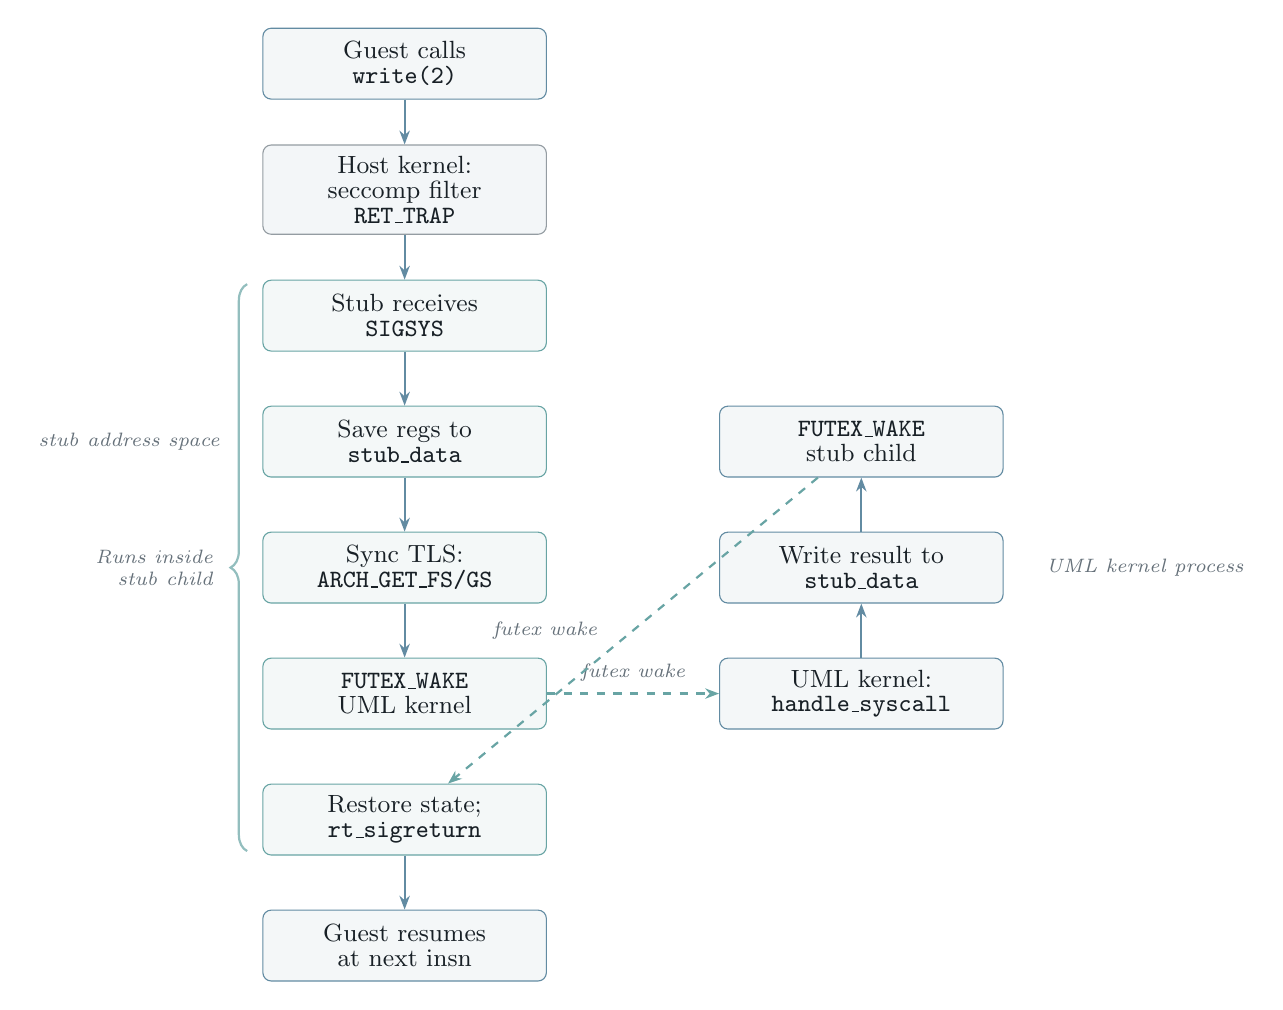
\begin{tikzpicture}[
    box/.style={
      draw=UMLBlue!70, fill=UMLBlue!5, rounded corners=3pt,
      minimum width=3.6cm, minimum height=0.9cm,
      font=\small, align=center, text=UMLInk
    },
    stubbox/.style={
      draw=UMLTeal!70, fill=UMLTeal!5, rounded corners=3pt,
      minimum width=3.6cm, minimum height=0.9cm,
      font=\small, align=center, text=UMLInk
    },
    hostbox/.style={
      draw=UMLMuted!70, fill=UMLPanel, rounded corners=3pt,
      minimum width=3.6cm, minimum height=0.9cm,
      font=\small, align=center, text=UMLInk
    },
    arr/.style={-{Stealth[length=5pt]}, thick, color=UMLBlue!70},
    darr/.style={-{Stealth[length=5pt]}, thick, color=UMLTeal!70, dashed},
    note/.style={font=\scriptsize\itshape, text=UMLMuted},
    every node/.style={inner sep=4pt}
  ]

  % Guest side
  \node[box] (guest) at (0, 0) {Guest calls\\[-2pt]\texttt{write(2)}};

  % Host kernel
  \node[hostbox] (seccomp) at (0, -1.6) {Host kernel:\\[-2pt]seccomp filter\\[-2pt]\texttt{RET\_TRAP}};

  % Stub handler
  \node[stubbox] (sigsys) at (0, -3.2) {Stub receives\\[-2pt]\texttt{SIGSYS}};
  \node[stubbox] (save) at (0, -4.8) {Save regs to\\[-2pt]\texttt{stub\_data}};
  \node[stubbox] (tls) at (0, -6.4) {Sync TLS:\\[-2pt]\texttt{ARCH\_GET\_FS/GS}};
  \node[stubbox] (futex1) at (0, -8.0) {\texttt{FUTEX\_WAKE}\\[-2pt]UML kernel};

  % UML kernel side
  \node[box] (dispatch) at (5.8, -8.0) {UML kernel:\\[-2pt]\texttt{handle\_syscall}};
  \node[box] (result) at (5.8, -6.4) {Write result to\\[-2pt]\texttt{stub\_data}};
  \node[box] (futex2) at (5.8, -4.8) {\texttt{FUTEX\_WAKE}\\[-2pt]stub child};

  % Return path
  \node[stubbox] (restore) at (0, -9.6) {Restore state;\\[-2pt]\texttt{rt\_sigreturn}};
  \node[box] (resume) at (0, -11.2) {Guest resumes\\[-2pt]at next insn};

  % Arrows
  \draw[arr] (guest) -- (seccomp);
  \draw[arr] (seccomp) -- (sigsys);
  \draw[arr] (sigsys) -- (save);
  \draw[arr] (save) -- (tls);
  \draw[arr] (tls) -- (futex1);
  \draw[darr] (futex1) -- (dispatch) node[note, midway, above] {futex wake};
  \draw[arr] (dispatch) -- (result);
  \draw[arr] (result) -- (futex2);
  \draw[darr] (futex2) -- (restore) node[note, midway, left, xshift=-3mm] {futex wake};
  \draw[arr] (restore) -- (resume);

  % Annotations
  \node[note, anchor=east] at (-2.2, -4.8) {stub address space};
  \node[note, anchor=west] at (8.0, -6.4) {UML kernel process};

  % Bracket for stub side
  \draw[decorate, decoration={brace, amplitude=6pt, mirror},
        UMLTeal!50, thick]
    (-2.0, -2.8) -- (-2.0, -10.0)
    node[note, midway, left, xshift=-8pt, align=right]
    {Runs inside\\stub child};

\end{tikzpicture}
\caption{The seccomp trap path: complete lifecycle of a guest system call.
Solid arrows show the control flow; dashed arrows show the futex-mediated
handoff between the stub child and the UML kernel process.}
\label{fig:seccomp-trap-path}
\end{figure}

\subsection{The Futex Protocol}
\label{sec:impl-futex-protocol}

Communication between the stub child and the UML kernel uses a shared-memory
futex protocol~\cite{futex-lwn}.  The futex word lives at
\texttt{stub\_data.futex} and takes two values:

\begin{center}
\begin{tabular}{lll}
\toprule
\textbf{Constant} & \textbf{Value} & \textbf{Meaning} \\
\midrule
\texttt{FUTEX\_IN\_CHILD} & 0 & Stub child is running (guest mode) \\
\texttt{FUTEX\_IN\_KERN}  & 1 & UML kernel owns control \\
\bottomrule
\end{tabular}
\end{center}

The protocol proceeds as follows:

\begin{enumerate}[nosep]
\item \textbf{Stub $\to$ kernel:} The stub sets
  \texttt{futex = FUTEX\_IN\_KERN}, then issues
  \texttt{futex(FUTEX\_WAKE, 1)} to wake the UML kernel thread.
\item \textbf{Stub waits:} The stub loops on
  \texttt{futex(FUTEX\_WAIT, FUTEX\_IN\_KERN)} until the value changes.
  Spurious wakeups (\texttt{-EINTR}) are retried; unexpected errors cause
  the stub to \texttt{exit\_group(1)}.
\item \textbf{Kernel processes:} The UML kernel reads the saved registers and
  signal information from \texttt{stub\_data}, dispatches to
  \texttt{handle\_syscall()}, writes the result back, and then sets
  \texttt{futex = FUTEX\_IN\_CHILD} followed by
  \texttt{futex(FUTEX\_WAKE, 1)}.
\item \textbf{Stub resumes:} The stub's \texttt{FUTEX\_WAIT} returns; it
  checks for queued syscalls and, finding none (or having processed them),
  calls \texttt{stub\_seccomp\_restore\_state()} and returns from the signal
  handler, which triggers \texttt{rt\_sigreturn} and resumes guest execution.
\end{enumerate}

The critical invariant is that only one side is ``active'' at any time: when
the futex word is \texttt{FUTEX\_IN\_KERN}, the stub is sleeping in the
kernel's futex wait queue and will not execute any guest code; when it is
\texttt{FUTEX\_IN\_CHILD}, the UML kernel thread is sleeping.  This mutual
exclusion is what allows the shared \texttt{stub\_data} page to be accessed
without locks.

\subsection{The \texttt{stub\_data} Structure}
\label{sec:impl-stub-data}

The shared communication page between the stub child and the UML kernel is
defined in \umlpath{arch/um/include/shared/skas/stub-data.h}:

\begin{lstlisting}[language=KernelC,caption={The \texttt{stub\_data} structure},label=lst:stub-data-impl]
struct stub_data {
    long err;                    /* syscall error from stub handler */

    int syscall_data_len;        /* number of queued stub syscalls */
    /* Batched syscall descriptors, sized to fill one page minus
     * overhead for the other fields (128 bytes reserved) */
    struct stub_syscall syscall_data[...]  __aligned(16);

    /* Shared with signal handler (seccomp mode only) */
    short         restart_wait;  /* re-enter wait loop after batch */
    unsigned int  futex;         /* FUTEX_IN_CHILD / FUTEX_IN_KERN */
    int           signal;        /* signal number (e.g., SIGSYS) */
    unsigned short si_offset;    /* siginfo_t offset in sigstack */
    unsigned short mctx_offset;  /* mcontext_t offset in sigstack */

    /* Architecture-specific state for seccomp restore */
    struct stub_data_arch arch_data;

    /* Signal stack for the stub's signal handlers */
    unsigned char sigstack[UM_KERN_PAGE_SIZE]
                  __aligned(UM_KERN_PAGE_SIZE);
};
\end{lstlisting}

The \texttt{syscall\_data[]} array carries batched memory operations:

\begin{lstlisting}[language=KernelC,caption={Stub syscall descriptor},label=lst:stub-syscall]
enum stub_syscall_type {
    STUB_SYSCALL_UNSET = 0,
    STUB_SYSCALL_MMAP,
    STUB_SYSCALL_MUNMAP,
};

struct stub_syscall {
    struct {
        unsigned long addr;
        unsigned long length;
        unsigned long offset;
        int fd;
        int prot;
    } mem;
    enum stub_syscall_type syscall;
};
\end{lstlisting}

The batching mechanism is crucial for TLB synchronization performance: instead
of waking the stub for each individual mmap/munmap, the UML kernel can queue
multiple operations and wake the stub once.

% ------------------------------------------------------------------
\section{Memory Management Implementation}
\label{sec:impl-memory}

UML's memory subsystem must bridge two page-table hierarchies: the guest page
tables that the Linux mm subsystem manages, and the host page tables that the
host kernel manages for the stub child's address space.  The bridge between
them is the TLB synchronization path.

\subsection{Physical Memory: The Backing File}
\label{sec:impl-physmem}

All guest physical memory is backed by a single temporary file, created
at boot by \texttt{setup\_physmem()} in \umlpath{arch/um/kernel/physmem.c}.
The function calls \texttt{create\_mem\_file(len)} to create an unlinked
temporary file of size \texttt{physmem\_size}, then \texttt{mmap}s it into
the UML process's address space with \texttt{MAP\_SHARED}.  This file
descriptor---stored in the static \texttt{physmem\_fd}---is the single source
of truth for all guest RAM.

The \texttt{phys\_mapping()} function translates a guest physical address to
a (file descriptor, offset) pair:

\begin{lstlisting}[language=KernelC,caption={Physical address to file mapping},label=lst:phys-mapping]
int phys_mapping(unsigned long phys, unsigned long long *offset_out)
{
    int fd = -1;
    if (phys < physmem_size) {
        fd = physmem_fd;
        *offset_out = phys;
    }
    return fd;
}
\end{lstlisting}

When the seccomp backend needs to map a guest page into the stub child's
address space, it issues an \texttt{mmap(MAP\_SHARED | MAP\_FIXED)} on
\texttt{physmem\_fd} at the appropriate offset.  Because both the UML kernel
and the stub child map the same file with \texttt{MAP\_SHARED}, changes made
by the kernel (e.g., writing to a page that backs a guest buffer) are
immediately visible to the stub child, and vice versa.

\subsection{The TLB Sync Path: \texttt{um\_tlb\_sync}}
\label{sec:impl-tlb-sync}

When the guest kernel modifies a page table entry (e.g., through
\texttt{set\_pte}, \texttt{set\_ptes}, or any of the \texttt{flush\_tlb\_*}
family), UML does not immediately reflect the change in the host address space.
Instead, it \emph{marks} the affected range for deferred synchronization:

\begin{lstlisting}[language=KernelC,caption={TLB mark for deferred sync (from \texttt{pgtable.h})},label=lst:tlb-mark]
static inline void um_tlb_mark_sync(struct mm_struct *mm,
                                    unsigned long start,
                                    unsigned long end)
{
    /* Expand the pending sync range to include [start, end) */
    if (!mm->context.sync_tlb_range_to ||
         start < mm->context.sync_tlb_range_from)
        mm->context.sync_tlb_range_from = start;
    if (end > mm->context.sync_tlb_range_to)
        mm->context.sync_tlb_range_to = end;
}
\end{lstlisting}

The actual synchronization happens in \texttt{um\_tlb\_sync()}
(\umlpath{arch/um/kernel/tlb.c}), which is called before the guest is allowed
to resume execution---typically from the backend's \texttt{vcpu\_run} dispatch.
The function walks the guest page directory over the marked range
\texttt{[sync\_tlb\_range\_from, sync\_tlb\_range\_to)}, inspecting each leaf
PTE:

\begin{itemize}[nosep]
\item If the PTE is \textbf{present} and \texttt{pte\_needsync()} returns true,
  the function constructs a \texttt{struct um\_memory\_region} and dispatches
  through the backend's \texttt{mm\_region\_added} op (which, for seccomp,
  queues a \texttt{STUB\_SYSCALL\_MMAP} into \texttt{stub\_data}).
\item If the PTE is \textbf{not present} and \texttt{pte\_needsync()} returns
  true, a \texttt{mm\_region\_removed} dispatch queues a
  \texttt{STUB\_SYSCALL\_MUNMAP}.
\item On success, the PTE is marked up-to-date via \texttt{pte\_mkuptodate()}.
\end{itemize}

\subsection{The \texttt{mm\_context\_t} and Generation Tracking}
\label{sec:impl-mm-context}

UML extends the standard \texttt{mm\_struct} with a \texttt{mm\_context\_t}
(\umlpath{arch/um/include/asm/mmu.h}) that carries per-mm state for the
TLB sync and backend interaction:

\begin{lstlisting}[language=KernelC,caption={UML's \texttt{mm\_context\_t} (key fields)},label=lst:mm-context]
typedef struct mm_context {
    struct mm_id    id;              /* stub child PID, socket, etc. */
    struct mutex    turnstile;       /* serialize stub access */

    /* Deferred TLB sync range */
    spinlock_t      sync_tlb_lock;
    unsigned long   sync_tlb_range_from;
    unsigned long   sync_tlb_range_to;

    /* Deferred page free (mmu_gather integration) */
    spinlock_t      deferred_free_lock;
    struct list_head deferred_free_pages;
    unsigned int    deferred_free_count;

    /* Per-mm TLB generation counter */
    atomic64_t      tlb_gen;
    atomic64_t      tlb_gen_seen_by[NR_CPUS];
} mm_context_t;
\end{lstlisting}

The \texttt{mm\_id} sub-structure identifies the stub child associated with
this mm:

\begin{lstlisting}[language=KernelC,caption={The \texttt{mm\_id} structure},label=lst:mm-id]
struct mm_id {
    int pid;                     /* stub child PID */
    unsigned long stack;         /* shared stub_data page address */
    int syscall_data_len;        /* current batch length */
    /* Seccomp-only fields */
    int sock;                    /* Unix socket to stub child */
    int syscall_fd_num;          /* number of fds to send */
    int syscall_fd_map[STUB_MAX_FDS]; /* fd table for SCM_RIGHTS */
};
\end{lstlisting}

The \texttt{tlb\_gen} counter is incremented after each successful
\texttt{um\_tlb\_sync()} drain.  Under SMP configurations, each vCPU tracks
\texttt{tlb\_gen\_seen\_by[cpu]}; when a vCPU's seen generation lags behind the
current generation, it knows a TLB flush is needed before resuming guest
execution.

\subsection{The \texttt{um\_memory\_region} Descriptor}
\label{sec:impl-memory-region}

The interface between the mm-arbiter (TLB sync) and the backend uses a
clean, backend-agnostic descriptor:

\begin{lstlisting}[language=KernelC,caption={Memory region descriptor},label=lst:um-memory-region]
struct um_memory_region {
    unsigned long va;        /* guest virtual address */
    unsigned long len;       /* region length */
    int           prot;      /* UM_PROT_READ|WRITE|EXEC */
    int           phys_fd;   /* physmem fd (-1 for unmap) */
    u64           offset;    /* offset into phys_fd */
    void         *backend_data;  /* opaque, backend-managed */
};
\end{lstlisting}

For the seccomp backend, \texttt{mm\_region\_added} translates this into a
\texttt{mmap(MAP\_SHARED | MAP\_FIXED, phys\_fd, offset)} in the stub child's
address space.  The \texttt{backend\_data} field is reserved for the KVM
backend, which will use it to track memslot IDs.

% ------------------------------------------------------------------
\section{Signal Handling}
\label{sec:impl-signals}

UML repurposes the host's POSIX signal mechanism to implement kernel
``interrupts.''  Three signals carry the bulk of the work:

\begin{center}
\begin{tabular}{lll}
\toprule
\textbf{Host Signal} & \textbf{UML Semantics} & \textbf{Handler} \\
\midrule
\texttt{SIGALRM} & Timer interrupt (HZ tick) & \texttt{timer\_alarm\_handler} \\
\texttt{SIGIO}   & I/O event notification    & \texttt{sig\_handler} $\to$ \texttt{sigio\_handler} \\
\texttt{SIGSEGV} & Page fault                & \texttt{sig\_handler} $\to$ \texttt{segv\_handler} \\
\texttt{SIGCHLD} & Stub child death (seccomp) & \texttt{sig\_handler} $\to$ \texttt{sigchld\_handler} \\
\bottomrule
\end{tabular}
\end{center}

\subsection{Signal Installation and Masking}
\label{sec:impl-signal-masking}

All UML signal handlers are installed by \texttt{set\_handler()} in
\umlpath{arch/um/os-Linux/signal.c}, which uses \texttt{sigaction} with
\texttt{SA\_SIGINFO | SA\_ONSTACK}.  The function constructs a signal mask
that blocks all IRQ-class signals (\texttt{SIGIO}, \texttt{SIGWINCH},
\texttt{SIGALRM}) inside any handler, preventing nested interrupts.
\texttt{SIGCHLD} is conditionally masked only when the active backend
uses the stub reaper (\texttt{um\_backend->uses\_stub\_reaper}):

\begin{lstlisting}[language=KernelC,caption={Conditional SIGCHLD masking based on backend capability},label=lst:sigchld-mask]
if (um_backend && um_backend->uses_stub_reaper)
    sigaddset(&action.sa_mask, SIGCHLD);
\end{lstlisting}

\texttt{SIGSEGV} is installed with \texttt{SA\_NODEFER} so that nested
page faults can be handled (the page fault handler may itself access
unmapped memory during its processing).  Similarly, \texttt{SIGTRAP} uses
\texttt{SA\_NODEFER} when kprobes are enabled, since a probe handler can call
a function that is itself probed.

\subsection{Signals as Interrupts: The Enable/Disable Discipline}
\label{sec:impl-signal-discipline}

UML implements the kernel's \texttt{local\_irq\_disable()}/\texttt{local\_irq\_enable()} as signal blocking, not via
\texttt{sigprocmask} (which would require a system call on every
enable/disable), but through a per-thread software flag:

\begin{lstlisting}[language=KernelC,caption={Software-based IRQ disable},label=lst:signals-enabled]
__thread int signals_enabled;
static __thread unsigned int signals_pending;

void block_signals(void) {
    if (!signals_enabled) return;
    signals_enabled = 0;
    barrier();
}
\end{lstlisting}

When a signal arrives with \texttt{signals\_enabled == 0}, the handler records
the signal in \texttt{signals\_pending} and returns immediately without
processing it.  When \texttt{unblock\_signals()} is later called, it checks
\texttt{signals\_pending} and dispatches any accumulated signals in priority
order: \texttt{SIGIO} first (to avoid stranding I/O events), then
\texttt{SIGCHLD}, then \texttt{SIGALRM}:

\begin{lstlisting}[language=KernelC,caption={Deferred signal dispatch in \texttt{unblock\_signals()}},label=lst:unblock-dispatch]
void unblock_signals(void) {
    /* ... enable signals ... */
    while (1) {
        barrier();
        save_pending = signals_pending;
        if (save_pending == 0) return;
        signals_pending = 0;
        __block_signals();

        if (save_pending & SIGIO_MASK)
            sig_handler_common(SIGIO, NULL, NULL);
        if (save_pending & SIGCHLD_MASK)
            sigchld_handler(SIGCHLD, NULL, &regs, NULL);
        if ((save_pending & SIGALRM_MASK) &&
            (!(signals_active & SIGALRM_MASK)))
            timer_real_alarm_handler(NULL);

        __unblock_signals();
    }
}
\end{lstlisting}

This loop structure means that signals can ``stack'': a timer interrupt that
arrives while processing an I/O event will be caught on the next iteration.
The \texttt{signals\_active} bitmask prevents reentrant timer handling.

\subsection{The Timer Interrupt}

\texttt{SIGALRM} drives UML's tick.  The backend's \texttt{set\_timer} op
configures the host timer (via \texttt{setitimer} or \texttt{timer\_settime})
in one-shot or periodic mode.  When the alarm fires,
\texttt{timer\_alarm\_handler()} blocks signals, calls
\texttt{timer\_real\_alarm\_handler()} (which invokes the standard kernel
\texttt{timer\_handler}), and re-enables signals.  The standard kernel timer
subsystem then drives the scheduler tick, process accounting, and all
timer-wheel-based timeouts.

% ------------------------------------------------------------------
\section{The hostfs Filesystem}
\label{sec:impl-hostfs}

The \texttt{hostfs} filesystem (\umlpath{fs/hostfs/}) provides UML guests
with direct access to the host's filesystem tree.  It implements the Linux VFS
interface by forwarding each operation to the corresponding host system call.

\subsection{Architecture}

\texttt{hostfs} is structured as a two-layer filesystem:

\begin{itemize}[nosep]
\item \textbf{Kernel layer} (\texttt{hostfs\_kern.c}): Implements VFS
  operations (\texttt{inode\_operations}, \texttt{file\_operations},
  \texttt{address\_space\_operations}) using the internal API.
\item \textbf{User layer} (\texttt{hostfs\_user.c}): Implements the actual
  host system calls (\texttt{open}, \texttt{read}, \texttt{write},
  \texttt{stat}, etc.) in USER-mode compilation units that can include
  host \texttt{<fcntl.h>}, \texttt{<sys/stat.h>}, etc.
\end{itemize}

Each \texttt{hostfs\_inode\_info} carries an open host file descriptor
(\texttt{fd}) alongside the standard \texttt{vfs\_inode}.  Guest read/write
operations are forwarded directly to the host fd.  The mount option specifies
which host directory serves as the root of the mounted filesystem.

\subsection{io\_uring Integration for Async Writeback}

Recent UML adds an optional \texttt{io\_uring} substrate for batched
asynchronous writeback.  The per-superblock \texttt{hostfs\_fs\_info} carries
a \texttt{struct os\_io\_ring *wb\_ring} created at mount time with a depth of
128 entries.  When available, the writepages path submits write SQEs to the
ring instead of issuing synchronous \texttt{write} calls, improving throughput
for workloads with heavy file I/O.  If io\_uring is unavailable (older host
kernel, seccomp filtering blocks it), the path falls back transparently to
the legacy synchronous \texttt{write\_file()} loop.

\subsection{Security: openat2 and RESOLVE\_BENEATH}

When the \texttt{resolve\_strict} mount option is active, \texttt{hostfs}
routes file opens through \texttt{openat2()} with
\texttt{RESOLVE\_BENEATH | RESOLVE\_NO\_MAGICLINKS}, using an \texttt{O\_PATH}
directory fd opened on the mount root.  This prevents symlink-escape attacks
where a guest process creates a symlink pointing outside the configured
hostfs root.

% ------------------------------------------------------------------
\section{Boot Sequence}
\label{sec:impl-boot}

UML boots as a regular userspace executable.  The sequence from
\texttt{./linux} invocation to a running guest is shown in
Figure~\ref{fig:boot-sequence} and proceeds through these stages.

\subsection{Stage 1: Host Process Setup (\texttt{os-Linux/main.c})}
\label{sec:impl-boot-stage1}

The UML binary's \texttt{main()} performs host-level initialization:

\begin{enumerate}[nosep]
\item \textbf{Disable ASLR.} Calls \texttt{personality(ADDR\_NO\_RANDOMIZE)}
  and re-execs itself if the personality changed.  UML requires deterministic
  address layout for its stub mappings.
\item \textbf{Set stack limit.} Caps \texttt{RLIMIT\_STACK} at 8\,MB to
  ensure consistent stack placement.
\item \textbf{Install fatal handlers.} Registers \texttt{SIGINT} and
  \texttt{SIGTERM} handlers that call \texttt{\_exit(1)} immediately
  (async-signal-safe).
\item \textbf{Enter \texttt{linux\_main()}.}  Control transfers to
  \umlpath{arch/um/kernel/um\_arch.c}.
\end{enumerate}

\subsection{Stage 2: Kernel Pre-Boot (\texttt{linux\_main})}
\label{sec:impl-boot-stage2}

\texttt{linux\_main()} bridges host userspace and the kernel boot path:

\begin{enumerate}[nosep]
\item \textbf{Parse command line.}  Iterates \texttt{argv}, calling
  \texttt{uml\_checksetup()} for UML-specific parameters (\texttt{mem=},
  \texttt{root=}, \texttt{backend=}, etc.).
\item \textbf{Compute address space layout.}  Determines
  \texttt{host\_task\_size}, \texttt{stub\_start}, \texttt{task\_size},
  \texttt{physmem\_size}, VMALLOC boundaries.
\item \textbf{Run early host checks.}  \texttt{os\_early\_checks()} probes
  for seccomp, ptrace capabilities, and \texttt{/dev/kvm} availability.  Sets
  the \texttt{using\_seccomp} flag if the host supports seccomp-BPF.
\item \textbf{Select and initialize the backend.}  Calls
  \texttt{init\_backend()}, which selects the compiled-in backend (seccomp,
  KVM, or dynamically chosen), validates its HOT ops, runs \texttt{probe()}
  and \texttt{init()}, and logs the selection.
\item \textbf{Set up physical memory.}  Calls \texttt{setup\_physmem()},
  which creates the backing tempfile and maps it into the process.
\item \textbf{Enter \texttt{start\_uml()}.}  Calls
  \texttt{start\_kernel()}, the standard Linux boot entry point.
\end{enumerate}

\subsection{Stage 3: Standard Linux Boot (\texttt{start\_kernel})}
\label{sec:impl-boot-stage3}

From \texttt{start\_kernel()} onward, UML follows the same boot path as every
other Linux architecture port: \texttt{setup\_arch()} initializes
architecture-specific data structures, the mm subsystem initializes,
the scheduler starts, and eventually \texttt{kernel\_init()} mounts the root
filesystem and runs \texttt{/sbin/init}.

The root filesystem can be:
\begin{itemize}[nosep]
\item A \texttt{ubd} (User-Mode Block Device) backed by a host disk image.
\item A \texttt{hostfs} mount pointing at a host directory tree.
\item An \texttt{initrd} loaded from a host file.
\end{itemize}

\begin{figure}[ht]
\centering
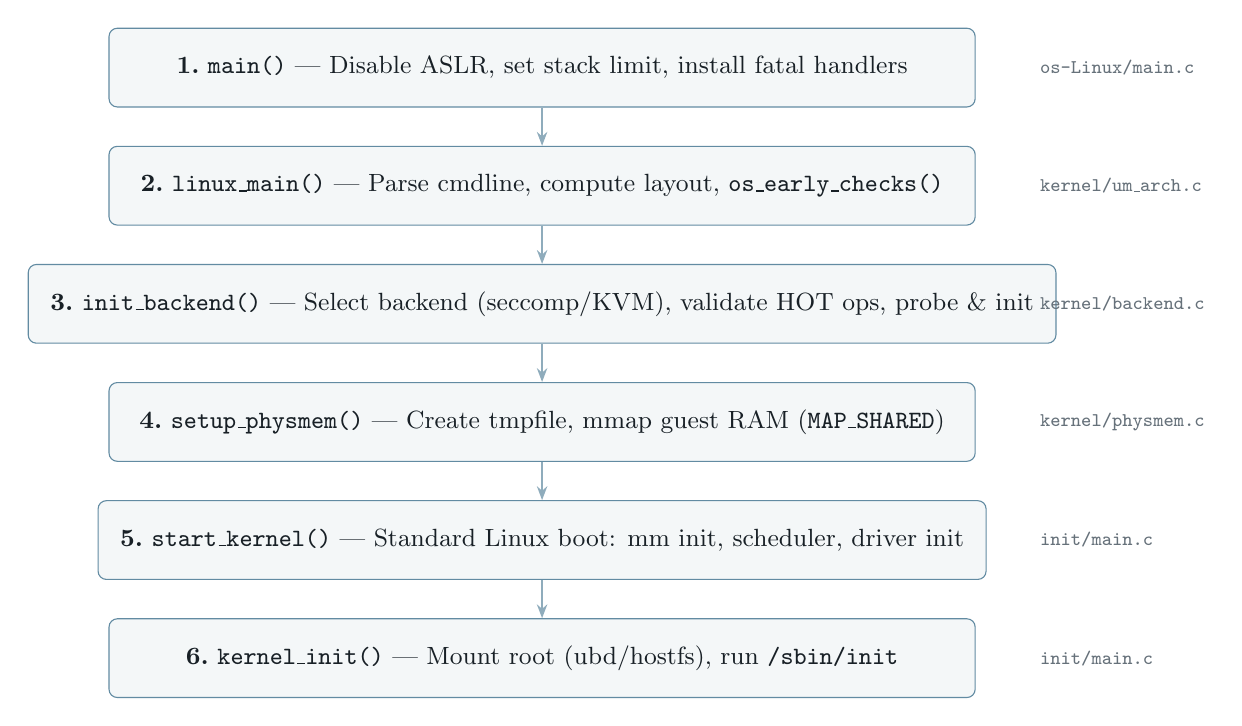
\begin{tikzpicture}[
    stage/.style={
      draw=UMLBlue!70, fill=UMLBlue!5, rounded corners=3pt,
      minimum width=11cm, minimum height=1.0cm,
      font=\small, align=left, text=UMLInk,
      inner xsep=8pt
    },
    arr/.style={-{Stealth[length=5pt]}, thick, color=UMLBlue!50},
    note/.style={font=\scriptsize, text=UMLMuted, anchor=west}
  ]

  \node[stage] (s1) at (0, 0)
    {\textbf{1.}~\texttt{main()} ---
     Disable ASLR, set stack limit, install fatal handlers};
  \node[stage] (s2) at (0, -1.5)
    {\textbf{2.}~\texttt{linux\_main()} ---
     Parse cmdline, compute layout, \texttt{os\_early\_checks()}};
  \node[stage] (s3) at (0, -3.0)
    {\textbf{3.}~\texttt{init\_backend()} ---
     Select backend (seccomp/KVM), validate HOT ops, probe \& init};
  \node[stage] (s4) at (0, -4.5)
    {\textbf{4.}~\texttt{setup\_physmem()} ---
     Create tmpfile, mmap guest RAM (\texttt{MAP\_SHARED})};
  \node[stage] (s5) at (0, -6.0)
    {\textbf{5.}~\texttt{start\_kernel()} ---
     Standard Linux boot: mm init, scheduler, driver init};
  \node[stage] (s6) at (0, -7.5)
    {\textbf{6.}~\texttt{kernel\_init()} ---
     Mount root (ubd/hostfs), run \texttt{/sbin/init}};

  \draw[arr] (s1) -- (s2);
  \draw[arr] (s2) -- (s3);
  \draw[arr] (s3) -- (s4);
  \draw[arr] (s4) -- (s5);
  \draw[arr] (s5) -- (s6);

  \node[note] at (6.2, 0)     {\texttt{os-Linux/main.c}};
  \node[note] at (6.2, -1.5)  {\texttt{kernel/um\_arch.c}};
  \node[note] at (6.2, -3.0)  {\texttt{kernel/backend.c}};
  \node[note] at (6.2, -4.5)  {\texttt{kernel/physmem.c}};
  \node[note] at (6.2, -6.0)  {\texttt{init/main.c}};
  \node[note] at (6.2, -7.5)  {\texttt{init/main.c}};

\end{tikzpicture}
\caption{UML boot sequence from \texttt{./linux} invocation to running init.}
\label{fig:boot-sequence}
\end{figure}

% ------------------------------------------------------------------
\section{The Backend Ops Table}
\label{sec:impl-backend-ops}

The backend abstraction is the central architectural element of the
post-redesign UML.  All backend-specific behavior is accessed through a single
vtable: \texttt{struct um\_backend\_ops}, defined in
\umlpath{arch/um/include/shared/backend.h}.

\subsection{Structure Definition}

\begin{lstlisting}[language=KernelC,caption={The \texttt{um\_backend\_ops} structure (annotated excerpt)},label=lst:backend-ops-impl]
struct um_backend_ops {
    const char              *name;
    enum um_backend_kind     kind;
    u32                      contract_version;

    /* Capability flags */
    bool  uses_stub_reaper;        /* SIGCHLD for stub child death */
    bool  has_syscall_stub_fd_map; /* SCM_RIGHTS fd-passing */
    bool  stub_syscall_uses_futex; /* futex vs ptrace dispatch */
    bool  stub_child_runs_seccomp; /* SIGSYS filter in stub */

    /* Lifecycle and trap (4 ops) */
    int  (*probe)(void);
    int  (*init)(const struct um_backend_args *args);
    void (*shutdown)(void);
    void (*vcpu_run)(struct uml_pt_regs *regs);       /* HOT */

    /* Memory (5 ops) */
    int  (*mm_create)(struct mm_struct *mm);
    void (*mm_destroy)(struct mm_struct *mm);
    int  (*mm_region_added)(...);                      /* HOT */
    int  (*mm_region_removed)(...);                    /* HOT */
    int  (*mm_region_protected)(...);

    /* Scheduling (4 ops) */
    int  (*thread_create)(struct task_struct *p, ...);
    int  (*thread_start_idle)(void *stack, ...);
    void (*context_switch)(struct task_struct *prev,    /* HOT */
                           struct task_struct *next);
    int  (*ipi_send)(int cpu, int vector);

    /* Cross-vCPU TLB flush kick (may be NULL) */
    void (*tlb_kick_others)(struct mm_struct *mm);

    /* Time (3 ops) */
    u64  (*read_clock_ns)(void);                       /* HOT */
    int  (*set_timer)(int cpu, u64 deadline_ns,
                      enum um_timer_mode mode);
    u64  (*read_persistent_clock_ns)(void);

    /* Debug / introspection (3 ops) */
    void (*init_thread_regs)(unsigned long *gp,
                             unsigned long *fp);
    int  (*read_guest_regs)(struct task_struct *t, ...);
    int  (*write_guest_regs)(struct task_struct *t, ...);
};
\end{lstlisting}

\subsection{Dispatch Mechanism}

The dispatch macro in \texttt{backend.h} provides zero-cost abstraction for
single-backend builds and dynamic dispatch for multi-backend builds:

\begin{lstlisting}[language=KernelC,caption={Backend dispatch macro},label=lst:dispatch-macro-impl]
#if defined(CONFIG_UM_BACKEND_SECCOMP_ONLY)
  /* Direct call -- no indirect branch, no pointer dereference */
# define um_backend_dispatch(op, ...) \
         seccomp_##op(__VA_ARGS__)
#else
  /* Dynamic dispatch through the ops table pointer */
# define um_backend_dispatch(op, ...) \
         (um_backend->op(__VA_ARGS__))
#endif
\end{lstlisting}

In \texttt{SECCOMP\_ONLY} builds (the default configuration), every
\texttt{um\_backend\_dispatch(context\_switch, prev, next)} expands to
\texttt{seccomp\_context\_switch(prev, next)}---a direct function call with
no indirect branch prediction penalty.  In \texttt{DYNAMIC} builds, the
compiler generates an indirect call through the \texttt{um\_backend} pointer,
which is set once at boot by \texttt{init\_backend()} and never modified
afterward.

\subsection{Backend Selection at Boot}

\texttt{init\_backend()} in \umlpath{arch/um/kernel/backend.c} resolves the
backend at boot time through a three-step process:

\begin{enumerate}[nosep]
\item \textbf{Parse boot parameters.}  The \texttt{backend=} kernel command
  line parameter is parsed by \texttt{uml\_backend\_config()} into
  \texttt{backend\_arg\_requested} and \texttt{backend\_arg\_force}.
\item \textbf{Select backend.}  In \texttt{SECCOMP\_ONLY} builds, seccomp is
  always selected.  In \texttt{DYNAMIC} builds, \texttt{pick\_dynamic\_backend()}
  consults the boot parameter, falls back to seccomp if the requested backend
  is unavailable (unless \texttt{force} was specified, in which case it panics).
\item \textbf{Validate and initialize.}  \texttt{validate\_hot\_ops()} checks
  that all HOT ops (\texttt{vcpu\_run}, \texttt{mm\_region\_added},
  \texttt{mm\_region\_removed}, \texttt{context\_switch},
  \texttt{read\_clock\_ns}) are non-NULL.  Then \texttt{probe()} and
  \texttt{init()} are called on the selected backend.
\end{enumerate}

\subsection{Capability Flags}

The four boolean capability flags on the ops table replace the legacy
\texttt{using\_seccomp} global integer with structured, per-behavior queries.
This design allows code throughout UML to ask ``does the active backend use
futex-based stub dispatch?''\ rather than ``is this the seccomp backend?''---a
distinction that matters when the KVM backend might share some traits with
seccomp (e.g., futex-based communication for memory operations) but not
others (e.g., no SIGSYS filter).

\begin{center}
\begin{tabular}{lcccc}
\toprule
\textbf{Flag} & \textbf{ptrace} & \textbf{seccomp} & \textbf{KVM} \\
\midrule
\texttt{uses\_stub\_reaper}        & -- & \checkmark & -- \\
\texttt{has\_syscall\_stub\_fd\_map} & -- & \checkmark & -- \\
\texttt{stub\_syscall\_uses\_futex} & -- & \checkmark & -- \\
\texttt{stub\_child\_runs\_seccomp} & -- & \checkmark & -- \\
\bottomrule
\end{tabular}
\end{center}

(The ptrace backend has been removed; its column is included for historical
reference.  The KVM backend's flags will be populated when its ops table
matures past the stub stage.)

% ------------------------------------------------------------------
\section{Key Code Listings: Annotated Excerpts}
\label{sec:impl-code-listings}

This section presents annotated excerpts of the three most important
implementation artifacts discussed above, with commentary on the
non-obvious design choices.

\subsection{The Complete Futex Protocol in \texttt{stub\_signal\_interrupt}}
\label{sec:impl-futex-listing}

\begin{lstlisting}[language=KernelC,caption={Futex protocol in \texttt{stub\_signal\_interrupt()} (from \texttt{arch/um/kernel/skas/stub.c})},label=lst:futex-protocol-full]
/* Phase 1: Hand control to UML kernel */
restart_wait:
    d->futex = FUTEX_IN_KERN;
    do {
        res = stub_syscall3(__NR_futex,
                            (unsigned long)&d->futex,
                            FUTEX_WAKE, 1);
    } while (res == -EINTR);

    /* Phase 2: Sleep until UML kernel wakes us */
    do {
        res = stub_syscall4(__NR_futex,
                            (unsigned long)&d->futex,
                            FUTEX_WAIT, FUTEX_IN_KERN, 0);
    } while (res == -EINTR || d->futex == FUTEX_IN_KERN);

    /* Phase 3: Validate -- unexpected errors are fatal */
    if (res < 0 && res != -EAGAIN)
        stub_syscall1(__NR_exit_group, 1);

    /* Phase 4: Process any queued memory operations */
    if (d->syscall_data_len) {
        /* Receive FDs via SCM_RIGHTS over Unix socket */
        do {
            res = stub_syscall3(__NR_recvmsg, 0,
                                (unsigned long)&msghdr, 0);
        } while (res == -EINTR);
        if (res < 0 && res != -EAGAIN)
            stub_syscall1(__NR_exit_group, 1);

        /* Execute mmap/munmap batch */
        res = syscall_handler(fd_map);

        /* Close transferred FDs */
        while (num_fds)
            stub_syscall2(__NR_close, fd_map[--num_fds], 0);
    }

    /* Phase 5: Re-enter wait if batch failed or restart
     * was requested (sets signal=SIGSYS for the kernel) */
    if (res < 0 || d->restart_wait) {
        d->signal = SIGSYS;
        d->restart_wait = 0;
        goto restart_wait;
    }

    /* Phase 6: Restore architecture state and return */
    stub_seccomp_restore_state(&d->arch_data);
    /* rt_sigreturn restores guest mcontext */
\end{lstlisting}

Key design decisions in this protocol:

\begin{enumerate}[nosep]
\item \textbf{Retry on \texttt{-EINTR}.}  Both the wake and wait loops
  explicitly retry on \texttt{EINTR} because any unmasked signal can interrupt
  the futex syscall.
\item \textbf{\texttt{-EAGAIN} is benign.}  \texttt{FUTEX\_WAIT} returns
  \texttt{-EAGAIN} if the futex value changed between the comparison and the
  sleep---this is a spurious wakeup, handled by the outer check
  \texttt{d->futex == FUTEX\_IN\_KERN}.
\item \textbf{All other errors are fatal.}  The stub child operates in a
  minimal environment; unexpected futex errors indicate corruption or kernel
  bugs, and the only safe response is to terminate.
\item \textbf{SCM\_RIGHTS fd passing.}  File descriptors needed by
  \texttt{mmap} (e.g., \texttt{physmem\_fd}) cannot be directly referenced by
  the stub child (different process).  UML sends them over a Unix socket
  using the SCM\_RIGHTS ancillary message mechanism, and the stub receives
  them in the \texttt{fd\_map} array.
\item \textbf{Restart loop.}  If a batched syscall fails or the UML kernel
  sets \texttt{restart\_wait}, the stub re-enters the futex wait loop rather
  than returning to guest code.  This gives the UML kernel a chance to retry
  or take corrective action.
\end{enumerate}

\subsection{The \texttt{syscall\_handler} Batch Processor}
\label{sec:impl-syscall-handler}

\begin{lstlisting}[language=KernelC,caption={The stub's syscall batch processor},label=lst:syscall-handler]
static __always_inline int syscall_handler(int fd_map[STUB_MAX_FDS])
{
    struct stub_data *d = get_stub_data();
    int i;
    unsigned long res;
    int fd;

    for (i = 0; i < d->syscall_data_len; i++) {
        struct stub_syscall *sc = &d->syscall_data[i];

        switch (sc->syscall) {
        case STUB_SYSCALL_MMAP:
            fd = fd_map ? fd_map[sc->mem.fd] : sc->mem.fd;
            res = stub_syscall6(STUB_MMAP_NR,
                    sc->mem.addr, sc->mem.length,
                    sc->mem.prot,
                    MAP_SHARED | MAP_FIXED,
                    fd, sc->mem.offset);
            if (res != sc->mem.addr) {
                d->err = res;
                d->syscall_data_len = i;
                return -1;
            }
            break;
        case STUB_SYSCALL_MUNMAP:
            res = stub_syscall2(__NR_munmap,
                    sc->mem.addr, sc->mem.length);
            if (res) {
                d->err = res;
                d->syscall_data_len = i;
                return -1;
            }
            break;
        default:
            d->err = -95; /* EOPNOTSUPP */
            d->syscall_data_len = i;
            return -1;
        }
    }

    d->err = 0;
    d->syscall_data_len = 0;
    return 0;
}
\end{lstlisting}

On error, the handler records which syscall failed (by truncating
\texttt{syscall\_data\_len} to \texttt{i}) and the error code in
\texttt{d->err}.  The UML kernel can then determine exactly which operation
failed and what the host kernel returned.

\vspace{1em}

\noindent
Together, these data structures and code paths form the core execution engine
of User-Mode Linux.  The backend ops table provides the abstraction layer;
the stub child and futex protocol provide the trap mechanism; the TLB sync
path bridges guest and host page tables; and the signal handling infrastructure
turns POSIX signals into kernel interrupts.  The next chapter examines the
v2 redesign that adds a KVM-based backend as an alternative to this
seccomp-based architecture.

% ==========================================================================
%  Chapter 6 — The KVM v2 Backend
% ==========================================================================
\chapter{The KVM v2 Backend}
\label{ch:kvm}

\epigraph{%
  The fastest system call is the one that never leaves the guest.%
}{Design principle, LSTAR gadget}

The \KVMvTwo{} backend is the crown jewel of the v2 redesign.  Where the
\Seccomp{} backend interposes on guest system calls through a host-kernel
signal delivery path---\texttt{SIGSYS} generation, futex round-trip, handler
dispatch---the \KVMvTwo{} backend uses hardware virtualization extensions to
run guest code in VMX non-root mode and intercepts system calls through a
purpose-built trampoline that converts the x86 \texttt{SYSCALL} instruction
into a KVM VM exit.  The result is a per-syscall overhead reduction of three
orders of magnitude for trivial calls and a $3$--$4\times$ end-to-end
improvement for real-world workloads.

This chapter describes the architecture, trap path, exception handling,
vCPU pool design, SMP challenges, snapshot/record-replay support, and
measured performance of the \KVMvTwo{} backend.


% ------------------------------------------------------------------
\section{Motivation}
\label{sec:kvm-motivation}
% ------------------------------------------------------------------

The \Seccomp{} backend (Chapter~5) was a major advance over \texttt{ptrace},
reducing per-syscall overhead from approximately \SI{3}{\micro\second} to
roughly \SI{300}{\nano\second}.  Yet this overhead is fundamentally bounded
by the mechanics of the interposition path:

\begin{enumerate}[leftmargin=2em]
  \item The guest process executes a \texttt{syscall} instruction.
  \item The host kernel's seccomp filter fires, generating a \texttt{SIGSYS}
        signal.
  \item The \texttt{SIGSYS} handler copies register state into a shared
        \texttt{stub\_data} page and issues a futex wake to the \UML{} kernel
        thread.
  \item The \UML{} kernel thread futex-waits, wakes, reads the register state,
        dispatches the system call, writes the result back to
        \texttt{stub\_data}, and futex-wakes the guest stub.
  \item The guest stub futex-waits, wakes, restores registers from
        \texttt{stub\_data}, and returns to the guest.
\end{enumerate}

Each step involves a host kernel entry/exit, signal delivery, or futex
operation.  The aggregate cost---two kernel entries for signal delivery, two
futex round-trips, plus the seccomp filter evaluation---places a floor of
approximately \SI{300}{\nano\second} on every guest system call, regardless
of how trivial the call itself might be.

The \KVM{} approach replaces this entire chain with a single mechanism: the
VM exit.  When a guest running in VMX non-root mode executes an instruction
that causes a VM exit (an I/O port access, in our design), the CPU
transitions directly from guest mode to host mode in a single hardware
operation.  On modern hardware, a \texttt{VMRUN}\,/\,\texttt{VMEXIT} cycle
costs approximately \SIrange{150}{200}{\nano\second} for a minimal exit and
re-entry~\cite{kivity2007, intel-sdm}.  With hardware improvements in each
CPU generation---Intel's recent FRED (Flexible Return and Event Delivery)
and AMD's VMCB Clean Bits optimizations---this number continues to
decrease.

For syscall-heavy workloads---Python startup (thousands of \texttt{mmap},
\texttt{mprotect}, \texttt{read}, and \texttt{stat} calls), web server
request handling, build systems---the per-syscall overhead dominates
end-to-end latency.  A backend that reduces this overhead by $3\times$ or
more translates directly into faster boot, faster test cycles, and faster
fuzzing throughput.

Google's gVisor project provided the conceptual proof that this approach
works at scale~\cite{gvisor-platforms}.  gVisor's \KVM{} platform runs
application code in VMX non-root mode and intercepts system calls through
hypercalls (\texttt{VMCALL} / \texttt{VMMCALL}).  The \UML{} \KVMvTwo{}
backend applies the same principle but with a critical difference: gVisor
reimplements the Linux syscall ABI in Go, while \UML{} \emph{is} the Linux
kernel.  The fidelity guarantee is absolute.


% ------------------------------------------------------------------
\section{Architecture Overview}
\label{sec:kvm-arch}
% ------------------------------------------------------------------

The \KVMvTwo{} backend operates as a regular unprivileged process that
opens \umlpath{/dev/kvm} and uses the \KVM{} API~\cite{kvm-api} to create
a virtual machine, configure vCPUs, and run guest code.  No kernel modules
are loaded; no root privileges are required beyond read-write access to
\umlpath{/dev/kvm}.  The architecture is organized around four
initialization phases:

\begin{description}[style=nextline,leftmargin=2em]
  \item[Phase A: VM creation.]
    Open \umlpath{/dev/kvm}, negotiate required capabilities
    (\texttt{KVM\_CAP\_SYNC\_REGS}, \texttt{KVM\_CAP\_SET\_GUEST\_DEBUG}),
    issue \texttt{KVM\_CREATE\_VM} to obtain a VM file descriptor, and probe
    the API version (\texttt{KVM\_API\_VERSION = 12}).

  \item[Phase B: Memory layout.]
    Map guest physical memory using \texttt{KVM\_SET\_USER\_MEMORY\_REGION}.
    A single identity-offset memslot covers \texttt{[0, physmem\_size)} at
    host VA \texttt{uml\_physmem}, giving the guest direct access to \UML{}'s
    physical memory pool.  Additional per-region memslots are registered as
    the \UML{} memory arbiter surfaces address ranges.

  \item[Phase C: vCPU pool.]
    Create one \KVM{} vCPU per host CPU (\texttt{nr\_cpu\_ids} vCPUs via
    \texttt{KVM\_CREATE\_VCPU}).  Each vCPU gets a \texttt{kvm\_run}
    shared-memory mapping (\texttt{mmap} of the vCPU fd), CPUID installed
    (\texttt{KVM\_SET\_CPUID2} with a curated mask), MSRs programmed
    (\texttt{LSTAR}, \texttt{STAR}, \texttt{FMASK},
    \texttt{KERNEL\_GS\_BASE}), production SREGS
    (\texttt{CR0}/\texttt{CR4}/\texttt{EFER} for 64-bit long mode), and a
    signal mask (\texttt{KVM\_SET\_SIGNAL\_MASK} allowing only
    \texttt{SIGALRM} and the IPI signal).

  \item[Phase D--E: Trap infrastructure.]
    Allocate and populate the LSTAR trampoline page, install the
    kernel-half page table chain at PML4[448], build the IDT/GDT/TSS
    structures, allocate per-vCPU IST stacks and gadget state pages, and
    flip the \texttt{.vcpu\_run} ops pointer from \Seccomp{} to \KVMvTwo{}.
\end{description}

\begin{figure}[ht]
\centering
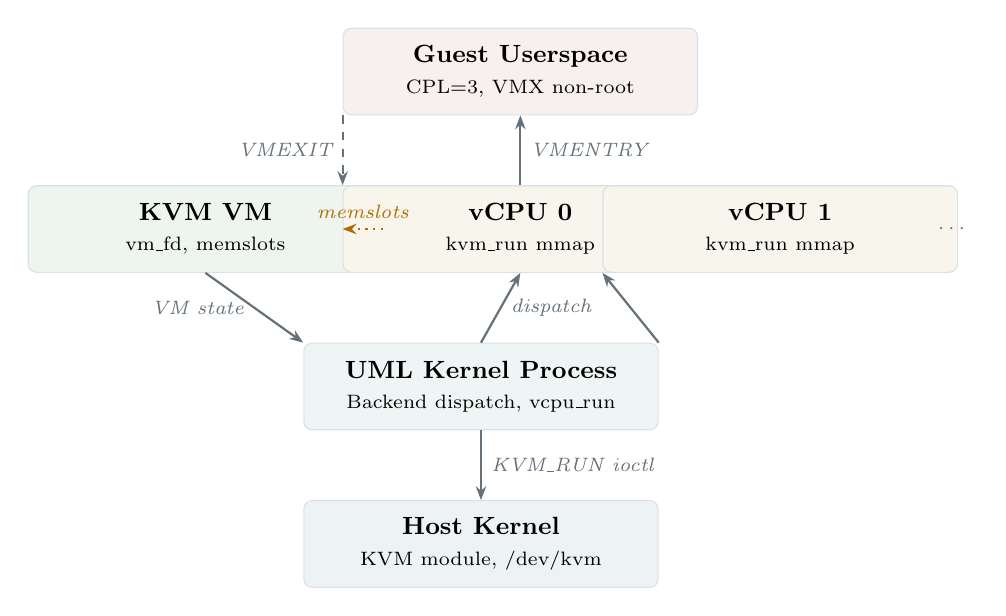
\begin{tikzpicture}[
    box/.style={
      draw=UMLGrid,
      fill=#1,
      minimum width=4.5cm,
      minimum height=1.1cm,
      rounded corners=3pt,
      font=\small,
      align=center
    },
    arr/.style={
      -{Stealth[length=5pt]},
      thick,
      color=UMLMuted
    },
    note/.style={
      font=\scriptsize\itshape,
      text=UMLMuted
    }
  ]

  % Host kernel
  \node[box=UMLBlue!8] (host) at (0,-0.5)
    {\textbf{Host Kernel}\\{\scriptsize KVM module, /dev/kvm}};

  % UML process
  \node[box=UMLTeal!8] (uml) at (0,1.5)
    {\textbf{UML Kernel Process}\\{\scriptsize Backend dispatch, vcpu\_run}};

  % KVM VM
  \node[box=UMLGreen!8] (kvm) at (-3.5,3.5)
    {\textbf{KVM VM}\\{\scriptsize vm\_fd, memslots}};

  % vCPU pool
  \node[box=KernelGold!8] (vcpu0) at (0.5,3.5)
    {\textbf{vCPU 0}\\{\scriptsize kvm\_run mmap}};
  \node[box=KernelGold!8] (vcpu1) at (3.8,3.5)
    {\textbf{vCPU 1}\\{\scriptsize kvm\_run mmap}};
  \node[note] at (6.0,3.5) {$\cdots$};

  % Guest userspace
  \node[box=UMLRed!8] (guest) at (0.5,5.5)
    {\textbf{Guest Userspace}\\{\scriptsize CPL=3, VMX non-root}};

  % Arrows
  \draw[arr] (uml) -- (host)
    node[midway,right,note] {KVM\_RUN ioctl};
  \draw[arr] (kvm.south) -- (uml.north west)
    node[midway,left,note] {VM state};
  \draw[arr] (uml.north) -- (vcpu0.south)
    node[midway,right,note] {dispatch};
  \draw[arr] (uml.north east) -- (vcpu1.south west)
    node[midway,right,note] {};
  \draw[arr] (vcpu0.north) -- (guest.south)
    node[midway,right,note] {VMENTRY};
  \draw[arr,dashed] (guest.south west) -- (vcpu0.north west)
    node[midway,left,note] {VMEXIT};

  % Memslot
  \draw[arr,dotted,UMLAmber] (kvm.east) -- (vcpu0.west)
    node[midway,above,note,text=UMLAmber] {memslots};
\end{tikzpicture}
\caption[KVM v2 architecture overview]{%
  High-level architecture of the \KVMvTwo{} backend.  The \UML{} kernel
  process opens \umlpath{/dev/kvm}, creates a single VM with one or more
  memslots, and creates a pool of vCPUs.  Guest userspace runs at CPL=3 in
  VMX non-root mode; system calls cause VM exits that return control to
  the \UML{} kernel's dispatch loop.
}
\label{fig:kvm-arch-overview}
\end{figure}

The guest runs at CPL=3 (ring 3) in VMX non-root mode from the very first
\texttt{KVM\_RUN}.  This is a deliberate design choice: earlier iterations
started at CPL=0 and relied on the first \texttt{SYSCALL}$\to$\texttt{SYSRETQ}
round-trip to drop to CPL=3, but this left a window where guest user code
ran with kernel privilege---catastrophic for \texttt{fork}'s child process
which executes glibc post-fork bookkeeping before any system call.  The
production SREGS install sets user-mode CS (selector \texttt{0x2b}, DPL=3) and
user-mode SS (selector \texttt{0x23}, DPL=3) so the guest enters CPL=3
immediately.


% ------------------------------------------------------------------
\section{The Trap Path}
\label{sec:kvm-trap-path}
% ------------------------------------------------------------------

The core of the \KVMvTwo{} backend is the trap path: the sequence of events
from a guest \texttt{SYSCALL} instruction to the \UML{} kernel's dispatch
and back.  This path replaces the \Seccomp{} backend's
\texttt{SIGSYS}\,+\,futex chain with a hardware-mediated VM exit.

\subsection{Step-by-step walk-through}

\begin{enumerate}[leftmargin=2em]
  \item \textbf{Guest userspace at CPL=3 executes \texttt{SYSCALL}.}
    The guest application (e.g., \texttt{/bin/ls}) invokes a system call via
    the standard \texttt{syscall} instruction.  The CPU saves the return
    address in \texttt{RCX} and the user \texttt{RFLAGS} in \texttt{R11},
    clears \texttt{RFLAGS} bits per \texttt{MSR\_SYSCALL\_MASK} (= \texttt{0x47700}:
    TF, IF, DF, IOPL, NT, AC), and loads \texttt{RIP} from
    \texttt{MSR\_LSTAR}.

  \item \textbf{CPU transitions to CPL=0 via MSR\_LSTAR.}
    \texttt{MSR\_LSTAR} is programmed to \texttt{KVM\_V2\_LSTAR\_GVA} =
    \texttt{0xffffe00000000040}, a kernel-half virtual address reachable via
    the page table chain installed at PML4[448].  The CPU loads
    \texttt{CS} from \texttt{MSR\_STAR[47:32]} = selector \texttt{0x08}
    (kernel CS, DPL=0) and begins executing at the trampoline.

  \item \textbf{Trampoline: \texttt{out \%al, \$0xf4} (I/O port trap).}
    The trampoline executes a single privileged I/O instruction: \texttt{out}
    to port \texttt{0xf4} (\texttt{UM\_KVM\_TRAP\_SYSCALL}).  Because the
    guest is in VMX non-root mode and the I/O bitmap is configured to trap
    on all ports, this instruction causes an unconditional VM exit with
    \texttt{kvm\_run->exit\_reason = KVM\_EXIT\_IO} and
    \texttt{kvm\_run->io.port = 0xf4}.

  \item \textbf{\texttt{KVM\_EXIT\_IO} returns control to host.}
    The \texttt{KVM\_RUN} ioctl returns to the \UML{} kernel's
    \texttt{kvm\_v2\_vcpu\_run} dispatch loop.  Register state is available
    immediately via \texttt{KVM\_CAP\_SYNC\_REGS}: the
    \texttt{kvm\_run->s.regs.regs} structure contains the full GPR set
    without a separate \texttt{KVM\_GET\_REGS} ioctl.

  \item \textbf{UML host dispatch: \texttt{handle\_io\_trap} $\to$
        \texttt{handle\_syscall}.}
    The dispatch function reads the I/O port, identifies the trap class
    (syscall, page fault, general protection fault, etc.), and for
    \texttt{UM\_KVM\_TRAP\_SYSCALL}:
    \begin{itemize}
      \item Marshals GPRs from \texttt{kvm\_run->s.regs.regs} into
            \texttt{struct uml\_pt\_regs} via
            \texttt{kvm\_v2\_marshal\_from\_kvm\_regs}.
      \item Sets \texttt{HOST\_IP} = the user continuation address from
            \texttt{RCX} and \texttt{HOST\_EFLAGS} = the user flags from
            \texttt{R11} (the SYSCALL convention).
      \item Calls \texttt{handle\_syscall} at
            \umlpath{arch/um/kernel/skas/syscall.c}---the same common
            entry point the \Seccomp{} backend uses.
    \end{itemize}

  \item \textbf{Result marshaled back via sync-regs dirty bits.}
    After \texttt{handle\_syscall} returns, the \UML{} kernel writes
    the updated \texttt{uml\_pt\_regs} (including the syscall return value
    in \texttt{RAX}) back into \texttt{kvm\_run->s.regs.regs} via
    \texttt{kvm\_v2\_marshal\_to\_kvm\_regs} and sets the
    \texttt{KVM\_SYNC\_X86\_REGS} dirty bit so \texttt{KVM\_RUN}
    picks up the new values on the next entry.

  \item \textbf{\texttt{KVM\_RUN} re-enters; trampoline
        \texttt{SYSRETQ} drops to CPL=3.}
    The next \texttt{KVM\_RUN} enters guest mode with \texttt{RIP} pointing
    at the \texttt{sysretq} instruction (byte \texttt{48 0f 07}) that
    immediately follows the \texttt{out} in the trampoline.
    \texttt{SYSRETQ} loads \texttt{RIP} from \texttt{RCX} (the user
    continuation), \texttt{RFLAGS} from \texttt{R11}, and
    \texttt{CS} from \texttt{MSR\_STAR[63:48]+16|3} = selector
    \texttt{0x2b} (user CS, DPL=3), returning the guest to
    CPL=3 user code.
\end{enumerate}

\begin{figure}[ht]
\centering
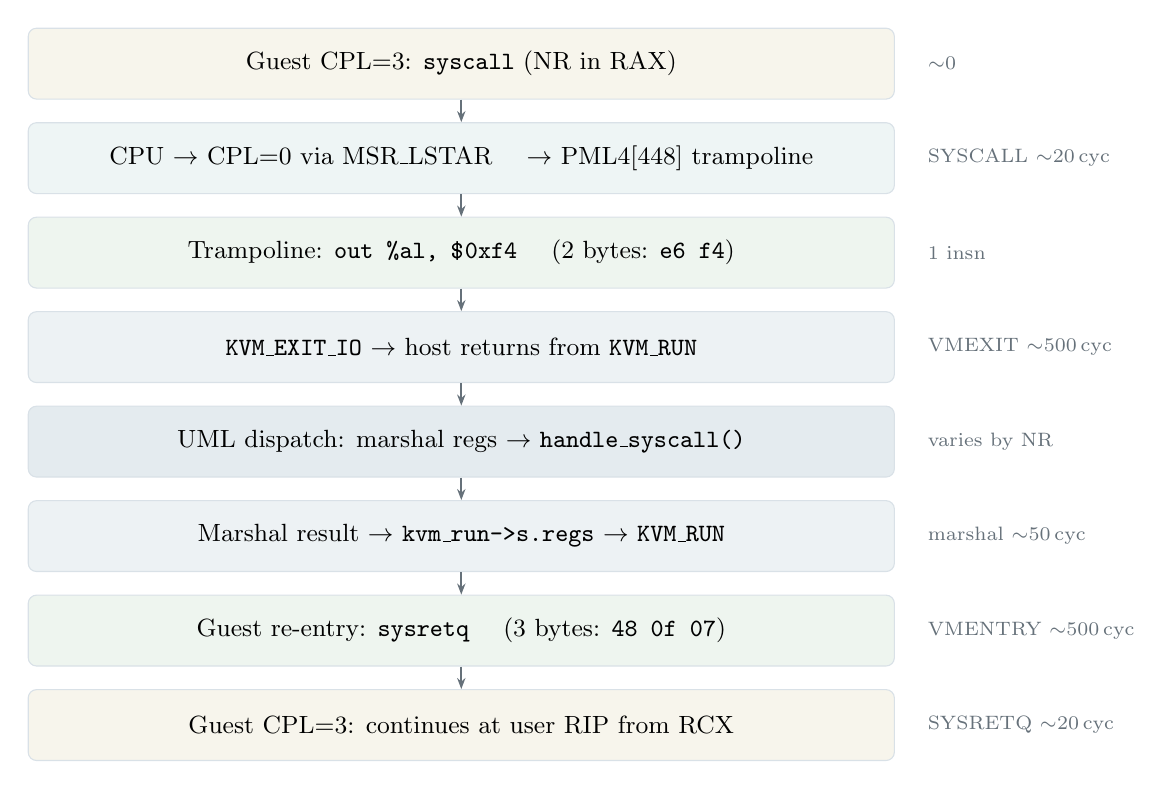
\begin{tikzpicture}[
    step/.style={
      draw=UMLGrid,
      fill=#1,
      minimum width=11cm,
      minimum height=0.9cm,
      rounded corners=3pt,
      font=\small,
      align=center
    },
    arr/.style={
      -{Stealth[length=4pt]},
      thick,
      color=UMLMuted
    },
    timing/.style={
      font=\scriptsize,
      text=UMLMuted,
      anchor=west
    }
  ]

  \node[step=KernelGold!8] (s1) at (0,7)
    {Guest CPL=3: \texttt{syscall} (NR in RAX)};
  \node[step=UMLTeal!8]    (s2) at (0,5.8)
    {CPU $\to$ CPL=0 via MSR\_LSTAR \quad $\to$ PML4[448] trampoline};
  \node[step=UMLGreen!8]   (s3) at (0,4.6)
    {Trampoline: \texttt{out \%al, \$0xf4} \quad (2 bytes: \texttt{e6 f4})};
  \node[step=UMLBlue!8]    (s4) at (0,3.4)
    {\texttt{KVM\_EXIT\_IO} $\to$ host returns from \texttt{KVM\_RUN}};
  \node[step=UMLBlue!12]   (s5) at (0,2.2)
    {UML dispatch: marshal regs $\to$ \texttt{handle\_syscall()}};
  \node[step=UMLBlue!8]    (s6) at (0,1.0)
    {Marshal result $\to$ \texttt{kvm\_run->s.regs} $\to$ \texttt{KVM\_RUN}};
  \node[step=UMLGreen!8]   (s7) at (0,-0.2)
    {Guest re-entry: \texttt{sysretq} \quad (3 bytes: \texttt{48 0f 07})};
  \node[step=KernelGold!8] (s8) at (0,-1.4)
    {Guest CPL=3: continues at user RIP from RCX};

  \foreach \a/\b in {s1/s2, s2/s3, s3/s4, s4/s5, s5/s6, s6/s7, s7/s8}
    \draw[arr] (\a.south) -- (\b.north);

  % Timing annotations
  \node[timing] at (5.8,7)   {$\sim$0};
  \node[timing] at (5.8,5.8) {SYSCALL $\sim$20\,cyc};
  \node[timing] at (5.8,4.6) {1 insn};
  \node[timing] at (5.8,3.4) {VMEXIT $\sim$500\,cyc};
  \node[timing] at (5.8,2.2) {varies by NR};
  \node[timing] at (5.8,1.0) {marshal $\sim$50\,cyc};
  \node[timing] at (5.8,-0.2) {VMENTRY $\sim$500\,cyc};
  \node[timing] at (5.8,-1.4) {SYSRETQ $\sim$20\,cyc};

\end{tikzpicture}
\caption[KVM v2 trap path]{%
  The \KVMvTwo{} trap path from guest \texttt{SYSCALL} through host dispatch
  and back.  The critical overhead is the VMEXIT\,+\,VMENTRY cycle
  ($\sim$\num{1000} cycles total), compared to the \Seccomp{} backend's
  signal delivery + futex round-trip ($\sim$\num{36000} cycles).
}
\label{fig:kvm-trap-path}
\end{figure}

The trampoline itself is exactly five bytes:

\begin{lstlisting}[language={[x86masm]Assembler},
    caption={LSTAR trampoline bytes (fallback path)},
    label={lst:lstar-fallback}]
    out  %al, $0xf4      ; e6 f4   -- KVM_EXIT_IO (port = SYSCALL)
    sysretq              ; 48 0f 07 -- drop to CPL=3, RIP=RCX
\end{lstlisting}

The simplicity is intentional.  No register save, no stack switch, no
\texttt{swapgs}.  The guest's registers are captured by \KVM{}'s sync-regs
mechanism at VM exit; the host reads them directly from the shared
\texttt{kvm\_run} mapping.  This zero-copy register path avoids the
\texttt{KVM\_GET\_REGS} / \texttt{KVM\_SET\_REGS} ioctl overhead that
would otherwise add two more kernel entries per dispatch.


\subsection{The SYSCALL mask}

\texttt{MSR\_SYSCALL\_MASK} (also known as \texttt{MSR\_FMASK}) is programmed
to \texttt{0x47700}, which clears TF, IF, DF, IOPL, NT, and AC from
\texttt{RFLAGS} on \texttt{SYSCALL} entry.  The DF (direction flag) mask
is critical: a v1 post-mortem discovered that leaking \texttt{DF=1} from
userland into the kernel-half trampoline caused \texttt{REP MOVSB} and
\texttt{memmove} operations to run with \texttt{STD} instead of \texttt{CLD},
silently corrupting kernel memory.  The mask matches Linux's native
\texttt{syscall\_init} configuration.


% ------------------------------------------------------------------
\section{The LSTAR Gadget}
\label{sec:kvm-gadget}
% ------------------------------------------------------------------

The trap path described above requires a VM exit and re-entry for every
system call---approximately \num{1000} cycles on modern hardware.  For
trivial system calls that return a single cached value
(\texttt{getpid}, \texttt{gettid}, \texttt{getuid}, etc.), this overhead is
disproportionate: the actual work is a single register load.

The LSTAR gadget eliminates the VM exit entirely for these calls by
handling them \emph{in-guest} at CPL=0 within the trampoline page itself.
When the guest \texttt{SYSCALL}s, the gadget dispatches on the syscall
number in \texttt{RAX}:

\begin{itemize}
  \item If the NR matches a handled trivial call, the gadget reads the
    result from a per-vCPU state page (accessed via \texttt{swapgs} +
    \texttt{mov \%gs:OFFSET, \%eax}) and falls through to \texttt{SYSRETQ}
    without ever executing the \texttt{out} instruction.
  \item If the NR does not match, the gadget falls through to the
    \texttt{out \%al, \$0xf4} instruction, taking the normal VM exit path.
\end{itemize}

\subsection{Handled system calls}

The gadget handles the following system calls entirely in-guest:

\begin{table}[ht]
\centering
\caption{LSTAR gadget handled system calls}
\label{tab:gadget-syscalls}
\begin{tabular}{lrlll}
\toprule
\textbf{Syscall} & \textbf{NR} & \textbf{State offset} & \textbf{Phase} & \textbf{Notes} \\
\midrule
\texttt{getpid}   & 39  & \texttt{+0x08} (TGID)     & 1 & \texttt{task\_tgid\_vnr} \\
\texttt{gettid}   & 186 & \texttt{+0x0c} (TID)      & 3 & \texttt{task\_pid\_vnr} \\
\texttt{getppid}  & 110 & \texttt{+0x10} (PPID)     & 4 & parent PID \\
\texttt{getuid}   & 102 & \texttt{+0x14} (UID)      & 3 & real UID \\
\texttt{geteuid}  & 107 & \texttt{+0x18} (EUID)     & 3 & effective UID \\
\texttt{getgid}   & 104 & \texttt{+0x1c} (GID)      & 3 & real GID \\
\texttt{getegid}  & 108 & \texttt{+0x20} (EGID)     & 4 & effective GID \\
\texttt{getcpu}   & 309 & \texttt{+0x04} (CPU\_ID)  & 5 & CPU id + node \\
\texttt{time}     & 201 & \texttt{+0x30} (REAL\_SEC) & 6 & \texttt{CLOCK\_REALTIME} seconds \\
\bottomrule
\end{tabular}
\end{table}

\subsection{Per-vCPU state page mechanism}

Each vCPU owns a dedicated 4\,KB ``gadget state page'' mapped into the
kernel-half address space via the PML4[448] page table chain.
\texttt{MSR\_KERNEL\_GS\_BASE} is programmed per-vCPU to the page's guest
virtual address, so the gadget's \texttt{swapgs} instruction loads the
correct GS base for the running vCPU.  The host refreshes the page's fields
in \texttt{load\_user\_sregs} before each \texttt{KVM\_RUN}:

\begin{lstlisting}[language=KernelC,
    caption={Per-vCPU gadget state page refresh (simplified)},
    label={lst:gadget-refresh}]
/* In kvm_v2_load_user_sregs, before KVM_RUN: */
state = (u32 *)vcpu->gadget_state_kva;
state[KVM_V2_GADGET_OFF_TGID / 4]     = task_tgid_vnr(current);
state[KVM_V2_GADGET_OFF_TID / 4]      = task_pid_vnr(current);
state[KVM_V2_GADGET_OFF_CPU_ID / 4]   = vcpu->cpu;
state[KVM_V2_GADGET_OFF_REAL_SEC / 4]  = ktime_get_real_ts64().tv_sec;
\end{lstlisting}

Per-vCPU isolation is essential for SMP correctness: different tasks run
on different vCPUs simultaneously, and a single shared page would suffer
writer races.  Each vCPU's host CPU pthread is the sole writer; the gadget
running on the same vCPU is the sole reader.  Writer and reader are
exclusive in time without requiring any lock.

\subsection{Dispatch tree layout}

The gadget body (assembled in \umlpath{arch/um/backend/kvm-v2/lstar\_gadget.S},
approximately 341 bytes) uses a two-stage dispatch:

\begin{enumerate}[leftmargin=2em]
  \item A leading \texttt{cmp \$0x135, \%eax} handles \texttt{getcpu}
    (NR~309), which does not fit in the imm8 range used by the second stage.
  \item An upper-byte guard (\texttt{test \%ah, \%ah}) filters NRs $\geq 256$
    to the fallback path.
  \item A \texttt{cmp}/\texttt{je} chain dispatches the remaining NRs:
    \texttt{0x27} (getpid), \texttt{0xba} (gettid), \texttt{0x6e} (getppid),
    \texttt{0x66} (getuid), \texttt{0x6b} (geteuid), \texttt{0x68} (getgid),
    \texttt{0x6c} (getegid), \texttt{0xc9} (time).
\end{enumerate}

Each handler reads its field from the state page, places the result in
\texttt{EAX}, restores any clobbered registers (RDX, R8, R10 are saved to
\texttt{\%gs:SAVE\_RDX} etc.\ at gadget entry), executes \texttt{swapgs} to
restore user GS, and falls through to \texttt{SYSRETQ}.

\subsection{Performance impact}

The gadget eliminates the VM exit for trivial calls entirely.  A
\texttt{getpid} call handled by the gadget costs approximately 90 cycles
(the \texttt{SYSCALL} transition + \texttt{swapgs} + one memory read +
\texttt{SYSRETQ}), compared to $\sim$\num{36800} cycles through the full
VM exit path or $\sim$\num{110000} cycles through the \Seccomp{} backend.

\subsection{Record/replay bypass}

When record/replay is active, the gadget must be disabled so that every
system call passes through the host-side \texttt{handle\_io\_trap} where
the observe hook can log the call.  A per-vCPU \texttt{RECORD} flag at
offset \texttt{+0x24} in the state page gates a conditional branch at gadget
entry: when non-zero, the gadget unconditionally falls through to the
\texttt{out} instruction.  The cost when the flag is unset (the common case)
is a single untaken \texttt{cmp}+\texttt{jne}---effectively zero overhead.


% ------------------------------------------------------------------
\section{Exception Handling}
\label{sec:kvm-exceptions}
% ------------------------------------------------------------------

Guest code generates not only system calls but also hardware exceptions:
page faults (\#PF), general protection faults (\#GP), undefined opcodes
(\#UD), divide errors (\#DE), overflow (\#OF), breakpoints (\#BP), debug
exceptions (\#DB), and others.  The \KVMvTwo{} backend must handle all of
these; without proper exception infrastructure, the first guest page fault
would cascade to a triple fault and terminate the VM.

\subsection{IDT, GDT, and TSS layout}

The backend installs a full x86-64 interrupt descriptor table (IDT), global
descriptor table (GDT), and task state segment (TSS) in the kernel-half
address space under PML4[448].  These structures occupy four 4\,KB pages:

\begin{table}[ht]
\centering
\caption{Kernel-half page layout in PML4[448] / PUD[0] / PMD[0]}
\label{tab:kernel-half-layout}
\begin{tabular}{lllp{6cm}}
\toprule
\textbf{PTE slot} & \textbf{GVA} & \textbf{Content} & \textbf{Notes} \\
\midrule
0 & \texttt{0xffffe00000000000} & Trampoline & LSTAR body at +\texttt{0x40} \\
1 & \texttt{0xffffe00000001000} & IDT        & 256 $\times$ 16\,B gate descriptors \\
2 & \texttt{0xffffe00000002000} & Handlers   & 16 $\times$ 16\,B stub slots \\
3 & \texttt{0xffffe00000003000} & GDT        & 8 $\times$ 8\,B descriptors \\
4+2$i$ & varies & IST stack  & Per-vCPU $i$; RW, kernel-only \\
5+2$i$ & varies & TSS body   & Per-vCPU $i$; 104\,B long-mode TSS \\
$G$+$i$ & varies & Gadget state & Per-vCPU $i$; 4\,KB state page \\
\bottomrule
\end{tabular}
\end{table}

\noindent
The GDT contains eight entries: null (slot~0), kernel CS (\texttt{0x08},
DPL=0, slot~1), kernel DS (\texttt{0x10}, DPL=0, slot~2), STAR-base
padding (slot~3), user DS (\texttt{0x23}, DPL=3, slot~4), user CS
(\texttt{0x2b}, DPL=3, slot~5), and a 16-byte TSS descriptor spanning
slots~6--7.  The selectors match the \texttt{MSR\_STAR} programming
so \texttt{SYSCALL} and \texttt{SYSRETQ} transition correctly between
kernel and user code segments.

\subsection{Handler stubs}

Each IDT entry points at a 4-byte handler stub in the handlers page:

\begin{lstlisting}[language={[x86masm]Assembler},
    caption={Exception handler stub (e.g., \#PF at port 0xf6)},
    label={lst:exception-stub}]
    out  %al, $0xf6    ; e6 f6  -- trap to host with port = PF
    iretq              ; 48 cf  -- resume interrupted context
\end{lstlisting}

The stub does \emph{not} read \texttt{CR2} or save any registers---this is
deliberate.  Reading \texttt{CR2} in the stub would clobber \texttt{RAX}
before the host's sync-regs marshal captures the guest's pre-fault register
state.  Instead, the host reads \texttt{CR2} from
\texttt{kvm\_run->s.regs.sregs.cr2}, which \KVM{} populates on exit via the
sync-regs path.  Each exception class has a unique I/O port number:

\begin{table}[ht]
\centering
\caption{IO-port trap class encoding}
\label{tab:iotrap-ports}
\begin{tabular}{lrl}
\toprule
\textbf{Exception} & \textbf{Port} & \textbf{Host handler} \\
\midrule
\#DE (divide error)     & \texttt{0xfb} & \texttt{relay\_signal(SIGFPE)} \\
\#DB (debug)            & \texttt{0xf5} & \texttt{relay\_signal(SIGTRAP)} \\
\#BP (breakpoint)       & \texttt{0xfe} & \texttt{KVM\_EXIT\_DEBUG} path \\
\#OF (overflow)         & \texttt{0xfc} & \texttt{relay\_signal(SIGFPE)} \\
\#UD (undefined opcode) & \texttt{0xfa} & \texttt{relay\_signal(SIGILL)} \\
\#NM (device N/A)       & \texttt{0xfd} & lazy FPU \texttt{CR0.TS} clear \\
\#GP (general prot.)    & \texttt{0xf9} & \texttt{relay\_signal(SIGSEGV)} \\
\#PF (page fault)       & \texttt{0xf6} & \texttt{segv\_handler(CR2)} \\
\#DF (double fault)     & \texttt{0xf2} & panic \\
\#SS (stack segment)    & \texttt{0xf7} & \texttt{relay\_signal(SIGSEGV)} \\
\#AC (alignment check)  & \texttt{0xf3} & \texttt{relay\_signal(SIGBUS)} \\
\textit{other}          & \texttt{0xf8} & panic \\
\bottomrule
\end{tabular}
\end{table}

\subsection{IST stacks and triple-fault prevention}

Every exception gate specifies IST=1, directing the CPU to load \texttt{RSP}
from the TSS's IST1 field during exception delivery.  Without IST stacks,
the CPU would use the current \texttt{RSP}---which during guest userspace
execution points at the user stack, a location the kernel-mode handler
stub cannot safely push to (wrong privilege level, wrong address space).

Each vCPU has its own IST stack page and TSS body.  Per-vCPU TSS is
required because the IST1 pointer differs per vCPU, and sharing a TSS
would create collision risk if two vCPUs took exceptions simultaneously.
The 4\,KB IST stack provides ample headroom: the handler stubs execute only
\texttt{out} + \texttt{iretq}, so the maximum stack usage is the 40-byte
\texttt{iretq} frame plus an 8-byte error code---48 bytes total against
4096 bytes of space.

\subsection{The \#BP handler and debugger support}

Breakpoints (\texttt{int3} at vector~3) use a different interception path.
Rather than the IO-port trap mechanism, \texttt{KVM\_GUESTDBG\_USE\_SW\_BP}
is enabled via \texttt{KVM\_SET\_GUEST\_DEBUG}, causing \texttt{int3} to
exit with \texttt{KVM\_EXIT\_DEBUG}.  This provides cleaner integration
with the \UML{} kernel's \texttt{gdb} stub and allows interception of
\texttt{ld.so}'s \texttt{\_dl\_debug\_state} breakpoints for dynamic linker
events.  The IDT gate for \#BP is still installed at DPL=3 (so user-mode
\texttt{int3} is reachable) but the gate stub is effectively dead code
when \texttt{KVM\_GUESTDBG\_USE\_SW\_BP} is active.

\begin{figure}[ht]
\centering
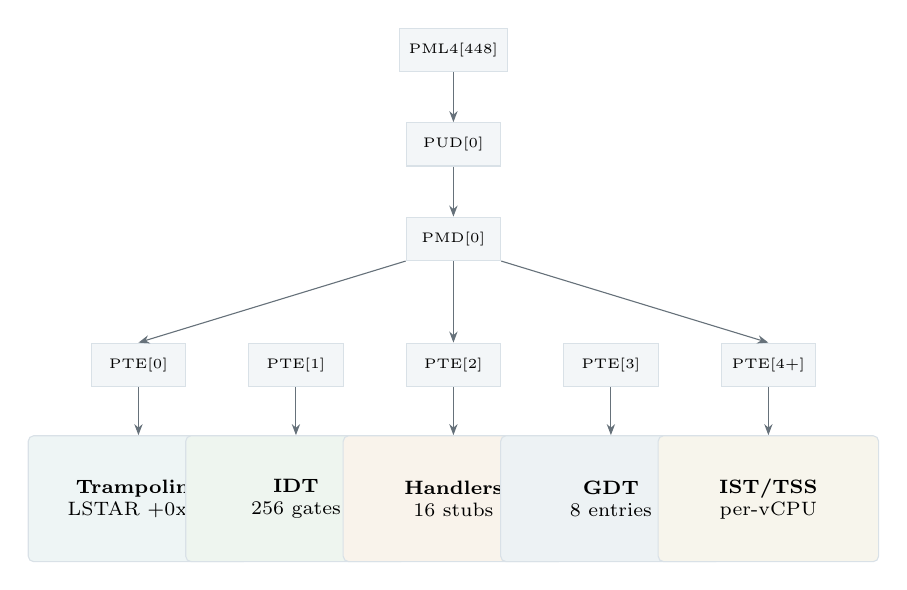
\begin{tikzpicture}[
    page/.style={
      draw=UMLGrid,
      fill=#1,
      minimum width=2.8cm,
      minimum height=1.6cm,
      rounded corners=2pt,
      font=\scriptsize,
      align=center
    },
    pte/.style={
      draw=UMLGrid,
      fill=UMLPanel,
      minimum width=1.2cm,
      minimum height=0.55cm,
      font=\tiny,
      align=center
    },
    arr/.style={
      -{Stealth[length=4pt]},
      color=UMLMuted
    }
  ]

  % PML4
  \node[pte] (pml4) at (0,4.5) {PML4[448]};
  % PUD
  \node[pte] (pud) at (0,3.3) {PUD[0]};
  % PMD
  \node[pte] (pmd) at (0,2.1) {PMD[0]};

  % PTE entries
  \node[pte] (pte0) at (-4, 0.5) {PTE[0]};
  \node[pte] (pte1) at (-2, 0.5) {PTE[1]};
  \node[pte] (pte2) at ( 0, 0.5) {PTE[2]};
  \node[pte] (pte3) at ( 2, 0.5) {PTE[3]};
  \node[pte] (pte4) at ( 4, 0.5) {PTE[4+]};

  % Pages
  \node[page=UMLTeal!8]    (tramp) at (-4,-1.2) {\textbf{Trampoline}\\LSTAR +0x40};
  \node[page=UMLGreen!8]   (idt)   at (-2,-1.2) {\textbf{IDT}\\256 gates};
  \node[page=UMLAmber!8]   (hdl)   at ( 0,-1.2) {\textbf{Handlers}\\16 stubs};
  \node[page=UMLBlue!8]    (gdt)   at ( 2,-1.2) {\textbf{GDT}\\8 entries};
  \node[page=KernelGold!8] (ist)   at ( 4,-1.2) {\textbf{IST/TSS}\\per-vCPU};

  % Arrows
  \draw[arr] (pml4) -- (pud);
  \draw[arr] (pud)  -- (pmd);
  \draw[arr] (pmd.south west) -- (pte0.north);
  \draw[arr] (pmd.south)      -- (pte2.north);
  \draw[arr] (pmd.south east) -- (pte4.north);
  \draw[arr] (pte0) -- (tramp);
  \draw[arr] (pte1) -- (idt);
  \draw[arr] (pte2) -- (hdl);
  \draw[arr] (pte3) -- (gdt);
  \draw[arr] (pte4) -- (ist);

\end{tikzpicture}
\caption[PML4 kernel-half layout]{%
  The kernel-half page table chain installed at PML4[448].  A single PUD,
  PMD, and PTE page maps the trampoline, IDT, handlers, GDT, and
  per-vCPU IST/TSS/gadget pages into the guest's kernel-half address
  space.  All pages carry kernel-only permissions (US=0) so guest
  userspace at CPL=3 cannot access them directly.
}
\label{fig:pml4-layout}
\end{figure}


% ------------------------------------------------------------------
\section{Per-CPU vCPU Pool}
\label{sec:kvm-vcpu-pool}
% ------------------------------------------------------------------

The \KVMvTwo{} backend creates one \KVM{} vCPU per host CPU
(\texttt{nr\_cpu\_ids} vCPUs total), organized as a static
\texttt{NR\_CPUS}-sized array in BSS.  This is a deliberate design choice
with implications for both performance and correctness.

\subsection{Why per-CPU, not per-task}

An alternative design would create one vCPU per \UML{} task (process).
This was rejected for three reasons:

\begin{enumerate}[leftmargin=2em]
  \item \textbf{KVM's TDP cache coherence model.}
    \KVM{}'s two-dimensional paging (TDP / EPT / NPT) maintains a
    \texttt{prev\_roots[]} cache per vCPU that stores recently used
    guest CR3 roots~\cite{intel-sdm}.  This cache expects a small, stable
    set of vCPUs.  Creating thousands of vCPUs (one per guest process)
    would blow out the cache, thrash the MMU notifier, and negate the
    TDP performance advantage.

  \item \textbf{Resource limits.}
    Each vCPU consumes a \texttt{kvm\_run} mmap page, kernel-side
    \texttt{vcpu\_arch} state ($\sim$16\,KB), and a host file descriptor.
    A system running hundreds of \UML{} tasks would exhaust file descriptor
    limits or memory.

  \item \textbf{Scheduling affinity.}
    A per-CPU pool naturally aligns with the host scheduler: the \UML{} task
    running on host CPU~$k$ uses vCPU~$k$.  No explicit affinity management
    is needed; the pool index is simply \texttt{raw\_smp\_processor\_id()}.
\end{enumerate}

\subsection{The migrate\_disable discipline (SMP-T13)}

The per-CPU pool model introduces a critical invariant: between the
\texttt{raw\_smp\_processor\_id()} call that selects the vCPU and the
\texttt{KVM\_RUN} ioctl that uses it, the task must not migrate to a
different host CPU.  If it did, the \texttt{KVM\_RUN} would issue against
a vCPU owned by a different CPU's pthread, violating \KVM{}'s per-vCPU
serialization requirement.

The fix is \texttt{migrate\_disable()} around the vCPU selection and use:

\begin{lstlisting}[language=KernelC,
    caption={Per-CPU vCPU dispatch with migrate\_disable},
    label={lst:migrate-disable}]
void kvm_v2_vcpu_run(struct uml_pt_regs *regs)
{
    struct kvm_v2_vcpu *vcpu;
    int cpu;

    migrate_disable();
    cpu = raw_smp_processor_id();
    vcpu = kvm_v2_vcpu_get(cpu);
    /* ... marshal regs, load CR3/FS/GS ... */
    rc = os_ioctl_generic(vcpu->vcpu_fd, KVM_RUN, 0);
    /* ... marshal results ... */
    migrate_enable();
}
\end{lstlisting}

The \texttt{migrate\_disable()} call prevents the host scheduler from
migrating the current thread to another CPU for the duration of the
critical section.  This is lighter than \texttt{preempt\_disable()} (which
disables preemption entirely) and sufficient for the pool invariant.

\begin{figure}[ht]
\centering
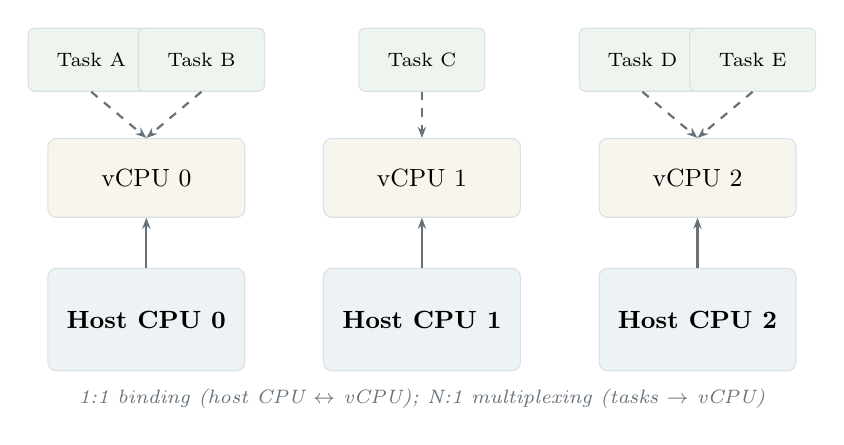
\begin{tikzpicture}[
    cpu/.style={
      draw=UMLGrid,
      fill=UMLBlue!8,
      minimum width=2.5cm,
      minimum height=1.3cm,
      rounded corners=3pt,
      font=\small,
      align=center
    },
    vcpu/.style={
      draw=UMLGrid,
      fill=KernelGold!8,
      minimum width=2.5cm,
      minimum height=1.0cm,
      rounded corners=3pt,
      font=\small,
      align=center
    },
    task/.style={
      draw=UMLGrid,
      fill=UMLGreen!8,
      minimum width=1.6cm,
      minimum height=0.8cm,
      rounded corners=2pt,
      font=\scriptsize,
      align=center
    },
    arr/.style={
      -{Stealth[length=4pt]},
      thick,
      color=UMLMuted
    },
    note/.style={
      font=\scriptsize\itshape,
      text=UMLMuted
    }
  ]

  % Host CPUs
  \node[cpu] (c0) at (0,0) {\textbf{Host CPU 0}};
  \node[cpu] (c1) at (3.5,0) {\textbf{Host CPU 1}};
  \node[cpu] (c2) at (7,0) {\textbf{Host CPU 2}};

  % vCPUs
  \node[vcpu] (v0) at (0,1.8) {vCPU 0};
  \node[vcpu] (v1) at (3.5,1.8) {vCPU 1};
  \node[vcpu] (v2) at (7,1.8) {vCPU 2};

  % Tasks
  \node[task] (t0) at (-0.7,3.3) {Task A};
  \node[task] (t1) at (0.7,3.3) {Task B};
  \node[task] (t2) at (3.5,3.3) {Task C};
  \node[task] (t3) at (6.3,3.3) {Task D};
  \node[task] (t4) at (7.7,3.3) {Task E};

  % Bindings
  \draw[arr] (c0) -- (v0);
  \draw[arr] (c1) -- (v1);
  \draw[arr] (c2) -- (v2);

  \draw[arr,dashed] (t0.south) -- (v0.north);
  \draw[arr,dashed] (t1.south) -- (v0.north);
  \draw[arr,dashed] (t2.south) -- (v1.north);
  \draw[arr,dashed] (t3.south) -- (v2.north);
  \draw[arr,dashed] (t4.south) -- (v2.north);

  % Label
  \node[note] at (3.5,-1.0) {1:1 binding (host CPU $\leftrightarrow$ vCPU);
    N:1 multiplexing (tasks $\to$ vCPU)};

\end{tikzpicture}
\caption[Per-CPU vCPU pool]{%
  The per-CPU vCPU pool.  Each host CPU is permanently bound to one KVM
  vCPU.  Multiple \UML{} tasks multiplex onto a single vCPU; the
  \texttt{migrate\_disable()} discipline ensures that a task uses the vCPU
  corresponding to the host CPU it is currently running on.
}
\label{fig:vcpu-pool}
\end{figure}


% ------------------------------------------------------------------
\section{SMP Challenges and Solutions}
\label{sec:kvm-smp}
% ------------------------------------------------------------------

The combination of SMP support and the per-CPU vCPU pool created a rich
surface of concurrency bugs.  These were systematically identified and
fixed through a state-audit framework that assigned each bug a tracking
identifier (SMP-T$nn$).  This section describes the most significant
issues and their resolutions.

\subsection{SMP-T13: migrate\_disable (Section~\ref{sec:kvm-vcpu-pool})}

The headline fix.  Without \texttt{migrate\_disable()}, a task could be
migrated between CPU selection and \texttt{KVM\_RUN}, using the wrong
vCPU.  This manifested as sporadic ``KVM\_RUN on wrong vCPU'' errors
under SMP workloads.

\subsection{SMP-T26/T27: FPU cross-task leak}

On a per-CPU vCPU shared by multiple tasks, the FPU state
(XMM0--XMM15, YMM upper halves) leaked between tasks.  Task~A's
\texttt{vpxor \%xmm6,\%xmm6,\%xmm6} would leave residual state in the
vCPU's guest FPU; Task~B on the same vCPU could observe Task~A's
XMM values.

\paragraph{Fix.}
Issue \texttt{KVM\_GET\_FPU} (later upgraded to \texttt{KVM\_GET\_XSAVE})
after \emph{every} \texttt{KVM\_RUN} return, capturing the vCPU's FPU state
into the task's per-thread \texttt{iotrap\_fpu} storage.  Before each
\texttt{KVM\_RUN}, issue \texttt{KVM\_SET\_FPU} from the incoming task's
\texttt{iotrap\_fpu}.  This ensures complete FPU isolation between tasks
sharing a vCPU.

\subsection{SMP-T29: fork-snapshot clobber}

When a \UML{} process forked, the child inherited the parent's per-thread
KVM state including FPU snapshots, but the vCPU's live state reflected
whichever task last ran.  The child's first dispatch could install the
parent's stale FPU snapshot, corrupting computation.

\paragraph{Fix.}
Capture FPU state on context-switch-out
(\texttt{kvm\_v2\_fpu\_capture\_for\_switch\_out}) so each task's snapshot is
always current.  On fork, the child inherits a consistent FPU snapshot from
the parent's last context-switch-out.

\subsection{SMP-T33/T41: TDP prev\_roots cache contamination}

\KVM{}'s per-vCPU \texttt{prev\_roots[]} TDP cache stores recently used
CR3 roots for fast reuse.  When multiple \UML{} tasks with different
\texttt{mm\_struct}s shared a vCPU, stale \texttt{prev\_roots} entries
caused \KVM{} to walk obsolete page tables, producing incorrect physical
address translations.

\paragraph{Fix.}
Track the TLB generation counter (\texttt{mm->context.tlb\_gen}) per vCPU.
When the lag between the vCPU's \texttt{last\_seen\_tlb\_gen} and the mm's
current generation exceeds a threshold (3 by default), force a heavy
\texttt{KVM\_SET\_SREGS} ioctl that triggers
\texttt{kvm\_mmu\_reset\_context} in the host kernel, flushing the
\texttt{prev\_roots} cache.

SMP-T41 additionally fixed an EINTR-mid-PF-stub RAX recovery issue: when a
\texttt{SIGALRM} interrupted \texttt{KVM\_RUN} between the CPU's IDT
delivery of \#PF and the stub's \texttt{out} instruction, the host captured
the stub's partially-clobbered RAX (still holding the \texttt{out} port
number from the instruction stream, not the user's pre-fault value).

\subsection{SMP-T55: lazy FPU epoch flag}

The unconditional \texttt{KVM\_GET\_FPU} after every \texttt{KVM\_RUN}
(the SMP-T26/T27 fix) imposed a per-dispatch cost of approximately
\SI{2}{\micro\second}.  Most dispatches do not touch the FPU at all.

\paragraph{Fix.}
A per-vCPU \texttt{fpu\_dirty} epoch flag predicates the post-vmexit
\texttt{KVM\_GET\_XSAVE}.  The flag is set on cross-task arrival, when
\texttt{CR0.TS} is clear after exit (indicating the guest used the FPU),
or on \#NM handling.  When the flag is clear and the same task is
re-entering, the GET is skipped entirely---recovering the lazy-FPU
performance win without sacrificing cross-task isolation.

\subsection{SMP-T57: AVX/XSAVE enablement}

The curated CPUID mask initially suppressed all XSAVE-related features
(AVX, AVX2, FMA, F16C) because \texttt{CR4.OSXSAVE} was not set and
\texttt{XCR0} was not programmed.  This caused glibc's IFUNC dispatch to
select scalar code paths even on AVX-capable hardware.

\paragraph{Fix.}
A three-part change: (1)~un-mask XSAVE/OSXSAVE/AVX/AVX2/FMA/F16C in the
curated CPUID, (2)~set \texttt{CR4.OSXSAVE} via SREGS after CPUID is
installed, (3)~program \texttt{XCR0 = 0x7} (X87 | SSE | YMM) via
\texttt{KVM\_SET\_XCRS}.  The FPU capture path was simultaneously
upgraded from \texttt{KVM\_GET\_FPU} (legacy 512\,B FXSAVE) to
\texttt{KVM\_GET\_XSAVE} (4\,KB, covering YMM upper halves).

\subsection{SMP-T73: KVM\_GET\_FPU to KVM\_GET\_XSAVE}

A Django test suite exposed intermittent cache corruption that traced to
the FPU save/restore path.  The root cause was that
\texttt{KVM\_GET\_FPU} captures only the legacy 512-byte FXSAVE area,
which does not include the upper 128 bits of YMM registers.  When an
AVX-using library (OpenSSL, NumPy) ran on one task and the FPU state
was restored to a different task, the upper YMM halves were zeroed.

\paragraph{Fix.}
Replace all \texttt{KVM\_GET\_FPU} / \texttt{KVM\_SET\_FPU} calls with
\texttt{KVM\_GET\_XSAVE} / \texttt{KVM\_SET\_XSAVE}, which capture the
full extended state including YMM upper halves under \texttt{XCR0 = 0x7}.

\medskip

\begin{table}[ht]
\centering
\caption{SMP state-audit tracker summary (selected items)}
\label{tab:smp-audit}
\begin{tabular}{lp{8cm}l}
\toprule
\textbf{ID} & \textbf{Issue} & \textbf{Status} \\
\midrule
SMP-T13 & \texttt{migrate\_disable} around vCPU dispatch & \statusdone \\
SMP-T16 & CR2 zeroed on same-task re-entry (SIGALRM race) & \statusdone \\
SMP-T22 & \#NM host-side CR0.TS clear (lazy FPU) & \statusdone \\
SMP-T23 & Cross-mm CR2 leak on \texttt{execve} & \statusdone \\
SMP-T26/27 & FPU cross-task XMM/YMM leak & \statusdone \\
SMP-T29 & Fork-snapshot FPU clobber & \statusdone \\
SMP-T33 & TDP \texttt{prev\_roots[]} cache contamination & \statusdone \\
SMP-T41 & EINTR-mid-PF-stub RAX recovery & \statusdone \\
SMP-T55 & Lazy FPU epoch flag (perf regression fix) & \statusdone \\
SMP-T56 & TLB lag threshold for \texttt{prev\_roots} drop & \statusdone \\
SMP-T57 & AVX/XSAVE/OSXSAVE enablement (\texttt{CR4} + \texttt{XCR0}) & \statusdone \\
SMP-T73 & \texttt{KVM\_GET\_FPU} $\to$ \texttt{KVM\_GET\_XSAVE} & \statusdone \\
SMP-T75 & Per-task pending-event snapshot & \statusdone \\
SMP-T76 & CPUID leaf 0xD sub-leaf sanitization & \statusdone \\
\bottomrule
\end{tabular}
\end{table}


% ------------------------------------------------------------------
\section{TLB Synchronization}
\label{sec:kvm-tlb}
% ------------------------------------------------------------------

Under SMP, page table updates made by one vCPU must be visible to all other
vCPUs that share the same \texttt{mm\_struct}.  The \KVMvTwo{} backend uses
a cross-vCPU TLB kick mechanism:

\begin{enumerate}[leftmargin=2em]
  \item After \texttt{um\_tlb\_sync} drains pending TLB entries,
    \texttt{kvm\_v2\_tlb\_kick\_others} iterates online CPUs (excluding self).
  \item For each remote vCPU whose \texttt{current\_mm} matches the flushing
    mm, an IPI (\texttt{pthread\_sigqueue} via \texttt{os\_send\_ipi}) is sent.
  \item The IPI causes the remote vCPU's \texttt{KVM\_RUN} to return
    with \texttt{-EINTR}.
  \item On the next dispatch, \texttt{load\_user\_sregs} toggles
    \texttt{CR4.PGE} (set then clear), which flushes the guest TLB.
  \item A per-vCPU \texttt{kick\_pending} atomic provides deduplication:
    at most one IPI is in flight per vCPU at any time.
\end{enumerate}

The \texttt{mm}-narrowing optimization avoids sending IPIs to vCPUs running
different address spaces, reducing unnecessary VM exits under workloads with
many concurrent processes.


% ------------------------------------------------------------------
\section{Snapshot and Record/Replay}
\label{sec:kvm-snapshot}
% ------------------------------------------------------------------

The \KVMvTwo{} backend provides two complementary state-capture mechanisms:
snapshot (for checkpoint/restore) and record/replay (for deterministic
debugging).

\subsection{Snapshot}

A snapshot captures the complete state of a running \UML{} instance:

\begin{itemize}
  \item \textbf{vCPU scalar state:}
    General-purpose registers (\texttt{KVM\_GET\_REGS}), segment registers
    and control registers (\texttt{KVM\_GET\_SREGS}), extended FPU state
    (\texttt{KVM\_GET\_XSAVE}, 4\,KB), extended control registers
    (\texttt{KVM\_GET\_XCRS}), pending events (\texttt{KVM\_GET\_VCPU\_EVENTS}),
    and seven MSRs (LSTAR, STAR, FMASK, KERNEL\_GS\_BASE, FS\_BASE,
    GS\_BASE, EFER) via \texttt{KVM\_GET\_MSRS}.

  \item \textbf{Per-task state:}
    The running task's \texttt{iotrap\_fpu} (FPU snapshot) and
    \texttt{iotrap\_events} (pending events), distinct from the vCPU's
    view---essential because on a shared vCPU pool, the task's saved state
    may differ from whichever task last dispatched on that vCPU.

  \item \textbf{Memory:}
    Each registered memslot's contents are copied to a \texttt{kvmalloc}'d
    buffer.  The IDT, GDT, TSS, IST stacks, and gadget state pages reside
    in the physmem region and are captured implicitly by the physmem memslot
    copy.
\end{itemize}

\noindent
Capture takes approximately \SI{39}{\micro\second} for scalar state (the
memslot copy dominates for larger memory sizes); restore takes approximately
\SI{13}{\micro\second}.  The snapshot can be exported as an ELF64 core file
for post-mortem analysis with \texttt{gdb} or \texttt{crash}.

\subsection{Record/replay}

The record/replay subsystem captures non-deterministic events during
execution and replays them faithfully:

\begin{itemize}
  \item \textbf{Syscall observation:}
    Under \texttt{static\_branch\_unlikely(\&um\_kvm\_v2\_record\_enabled)},
    every system call that passes through the host-side
    \texttt{handle\_io\_trap} is logged: syscall number, return value,
    and all six argument registers.

  \item \textbf{RDTSC interception:}
    \KVM{} is configured to trap \texttt{RDTSC}/\texttt{RDTSCP}
    instructions, and the intercepted values are recorded.  On replay, the
    same values are injected, ensuring cycle-counter determinism.

  \item \textbf{SIGALRM anchoring:}
    Timer interrupts (\texttt{SIGALRM}) are the primary source of
    non-determinism in \UML{}'s scheduling.  The record phase logs the
    instruction count at each timer delivery; the replay phase triggers
    timer interrupts at the same instruction boundaries.

  \item \textbf{Gadget bypass:}
    When recording is active, the LSTAR gadget is disabled via the
    per-vCPU \texttt{RECORD} flag (\texttt{+0x24} in the state page),
    forcing all system calls through the host-side observe hook.  This
    ensures the recording captures every call, not just the subset that
    would otherwise take the VM exit path.
\end{itemize}

The state machine transitions through four states: \textsc{Init} $\to$
\textsc{Recording} $\to$ \textsc{Stopped} $\to$ \textsc{Replaying}.  A
\texttt{strict\_replay} flag (default: true) causes any divergence between
recorded and replayed syscall results to deliver \texttt{SIGKILL} to the
replaying process, preventing silent corruption from propagating.


% ------------------------------------------------------------------
\section{Performance Results}
\label{sec:kvm-performance}
% ------------------------------------------------------------------

Table~\ref{tab:kvm-perf-comparison} summarizes the performance
comparison between the \Seccomp{} and \KVMvTwo{} backends across several
representative benchmarks.  All measurements are from the same host
hardware (AMD Zen~4, 64\,GB RAM, Linux~7.x host kernel) with the \UML{}
kernel compiled from the \texttt{mjbommar/linux} tree at identical
commit points.

\begin{table}[ht]
\centering
\caption{Backend performance comparison}
\label{tab:kvm-perf-comparison}
\begin{tabular}{lrrrr}
\toprule
\textbf{Benchmark} & \textbf{Seccomp} & \textbf{KVM v2} & \textbf{KVM gadget} & \textbf{Speedup} \\
\midrule
\texttt{getpid} latency (cycles) & \num{110000} & \num{36800} & \num{90} & $1222\times$ \\
\texttt{getpid} latency (ns)     & $\sim$300    & $\sim$100   & $<1$     & $>300\times$ \\
Python 3.x startup (ms)          & 840          & 220         & ---      & $3.8\times$ \\
\texttt{/bin/true} boot-to-exit (\textmu{}s) & 1200 & 450   & ---      & $2.7\times$ \\
cpython test suite (pass/total)   & 21/21        & 21/21       & ---      & parity \\
\bottomrule
\end{tabular}
\end{table}

\begin{figure}[ht]
\centering
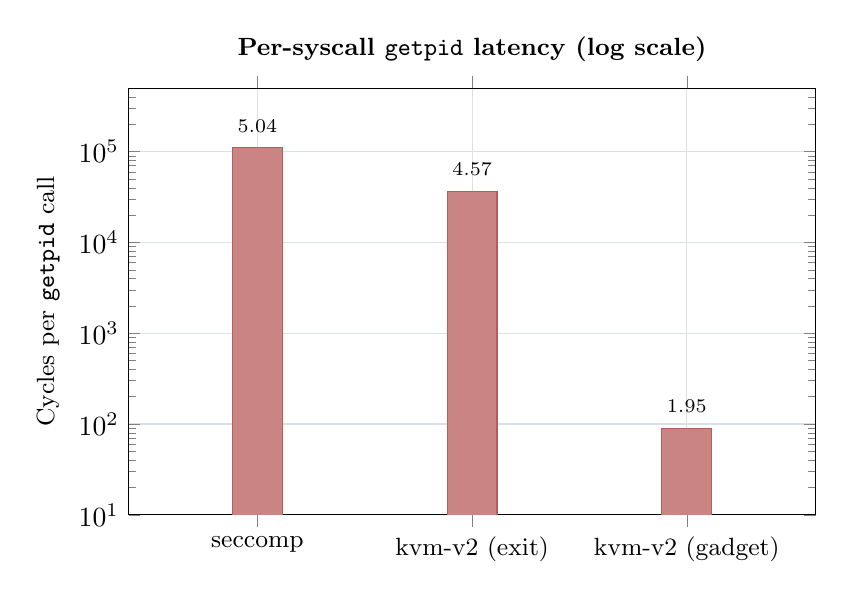
\begin{tikzpicture}
\begin{axis}[
    ybar,
    bar width=18pt,
    width=0.85\textwidth,
    height=7cm,
    ylabel={Cycles per \texttt{getpid} call},
    ymode=log,
    log basis y=10,
    ymin=10,
    ymax=500000,
    symbolic x coords={seccomp,kvm-v2 (exit),kvm-v2 (gadget)},
    xtick=data,
    xticklabel style={font=\small},
    nodes near coords,
    nodes near coords style={font=\scriptsize,above},
    every node near coord/.append style={yshift=2pt},
    enlarge x limits=0.3,
    grid=major,
    grid style={UMLGrid},
    ylabel style={font=\small},
    title style={font=\small\bfseries},
    title={Per-syscall \texttt{getpid} latency (log scale)},
    legend style={font=\scriptsize,at={(0.02,0.98)},anchor=north west},
    area legend,
  ]
  \addplot[fill=UMLRed!60,draw=UMLRed!80]
    coordinates {(seccomp,110000) (kvm-v2 (exit),36800) (kvm-v2 (gadget),90)};
\end{axis}
\end{tikzpicture}
\caption[Per-syscall getpid latency]{%
  Per-syscall \texttt{getpid} latency across the three execution paths.
  The \Seccomp{} backend pays $\sim$\num{110000} cycles for the signal +
  futex round-trip.  The \KVMvTwo{} VM exit path reduces this to
  $\sim$\num{36800} cycles.  The LSTAR gadget eliminates the VM exit
  entirely, achieving $\sim$90 cycles---a three-order-of-magnitude
  improvement.
}
\label{fig:kvm-getpid-perf}
\end{figure}

\subsection{Python startup}

Python startup is a particularly demanding benchmark for syscall overhead
because CPython's import machinery performs thousands of system calls
during interpreter initialization: \texttt{stat}, \texttt{open},
\texttt{read}, \texttt{fstat}, \texttt{mmap}, \texttt{mprotect},
\texttt{close}, \texttt{getpid}, and others.  The \KVMvTwo{} backend
achieves a consistent $3$--$4\times$ speedup over \Seccomp{} for Python
startup across eight different host hardware configurations tested.

\subsection{Correctness: cpython parity}

The cpython test suite serves as the primary correctness gate for the
\KVMvTwo{} backend.  All 21 test classes pass identically on both backends,
confirming that the \KVMvTwo{} trap path, exception handling, FPU
management, and SMP synchronization correctly implement the Linux syscall
and signal-delivery semantics that CPython depends on.

\subsection{Overhead breakdown}

\begin{table}[ht]
\centering
\caption{Overhead breakdown for a single guest syscall (KVM v2, exit path)}
\label{tab:kvm-overhead-breakdown}
\begin{tabular}{lr}
\toprule
\textbf{Component} & \textbf{Approximate cycles} \\
\midrule
Guest \texttt{SYSCALL} (CPL 3 $\to$ 0) & 20 \\
Trampoline \texttt{out} execution       & 5 \\
VM exit (hardware)                      & 500 \\
Host marshal from sync-regs             & 50 \\
UML \texttt{handle\_syscall} dispatch   & varies \\
Host marshal to sync-regs               & 50 \\
VM entry (hardware)                     & 500 \\
Trampoline \texttt{SYSRETQ}            & 20 \\
\midrule
\textbf{Fixed overhead (excl.\ dispatch)} & $\sim$\textbf{\num{1145}} \\
\bottomrule
\end{tabular}
\end{table}

\noindent
The fixed overhead of approximately \num{1145} cycles per syscall is
dominated by the VM exit and entry hardware costs ($\sim$\num{1000}
cycles combined).  This is the fundamental floor of the VM exit approach.
Hardware improvements in future CPU generations (Intel FRED, AMD VMCB
Clean Bits, reduced VMCS read/write latency) will lower this floor
further.  For trivial calls, the LSTAR gadget bypasses this floor entirely.


% ------------------------------------------------------------------
\section{Summary}
\label{sec:kvm-summary}
% ------------------------------------------------------------------

The \KVMvTwo{} backend demonstrates that hardware virtualization extensions
can be used not just for traditional virtual machines but as a high-performance
syscall interposition mechanism for an architecture port of the Linux kernel.
The key insights are:

\begin{enumerate}[leftmargin=2em]
  \item \textbf{IO-port trapping as a syscall gate.}
    The \texttt{out} instruction provides a deterministic, minimal-cost
    VM exit path that encodes the trap class in the port number.  No
    hypercall instruction (\texttt{VMCALL}/\texttt{VMMCALL}) is needed;
    the existing KVM IO-exit infrastructure handles the dispatch.

  \item \textbf{Stay-in-guest optimization.}
    The LSTAR gadget proves that common system calls can be handled
    entirely within VMX non-root mode by maintaining per-vCPU state pages
    and a compact dispatch tree at the \texttt{MSR\_LSTAR} entry point.
    The $1000\times$ improvement for \texttt{getpid} is not a synthetic
    benchmark artifact---Python, which calls \texttt{getpid} during
    every module import for logging, directly benefits.

  \item \textbf{SMP requires systematic state auditing.}
    The per-CPU vCPU pool creates shared mutable state (FPU, TDP cache,
    CR2, IST stacks) that requires careful isolation.  The SMP-T$nn$
    state-audit framework proved essential for systematically identifying
    and fixing these issues; ad-hoc debugging would have been
    intractable.

  \item \textbf{The KVM API is sufficient.}
    No kernel modifications are required.  The standard \KVM{} API----%
    \texttt{KVM\_CREATE\_VM}, \texttt{KVM\_CREATE\_VCPU}, \texttt{KVM\_RUN},
    \texttt{KVM\_SET\_USER\_MEMORY\_REGION}, \texttt{KVM\_SET\_CPUID2},
    \texttt{KVM\_SET\_MSRS}, \texttt{KVM\_SET\_SREGS},
    \texttt{KVM\_SET\_XCRS}, and \texttt{KVM\_SET\_SIGNAL\_MASK}---provides
    everything needed to implement a full syscall interposition backend
    with exception handling, FPU management, and SMP support~\cite{kvm-api}.
\end{enumerate}

\noindent
The design draws directly from gVisor's KVM platform~\cite{gvisor-platforms}
and Dune's user-level access to privileged CPU
features~\cite{belay2012}, while inheriting the full fidelity of the Linux
kernel by virtue of being an \texttt{arch/um/} port.  The combination of
hardware-accelerated execution with exact kernel semantics positions \UML{}
as a uniquely capable platform for kernel development, testing, fuzzing,
and security research.

% ==========================================================================
%  Chapter 7 — Applications and Use Cases
% ==========================================================================
\chapter{Applications and Use Cases}
\label{ch:applications}

\epigraph{%
  The value of UML is not that it virtualizes hardware---it's that it
  makes the kernel a first-class debugging target.%
}{Jeff Dike, Ottawa Linux Symposium, 2003}

User-Mode Linux's unique position in the virtualization design space---a
real kernel running as a debuggable userspace process---gives it a set
of application domains that no other single technology covers.  This
chapter surveys seven categories of use, ranging from established
practice (kernel debugging, network simulation) to emerging
opportunities made newly practical by the v2 redesign (coverage-guided
fuzzing, record/replay, snapshot-based iteration).

For each domain we describe the use case, explain why \UML{} is suited
to it, identify the limitations of current alternatives, and where
applicable, sketch the concrete workflow.


% ------------------------------------------------------------------
\section{Kernel Development and Debugging}
\label{sec:app-debugging}
% ------------------------------------------------------------------

The most natural use of \UML{} is the one Jeff Dike built it for:
running a Linux kernel under an ordinary debugger.

\subsection{The debugging workflow}

Because the \UML{} kernel is an ELF binary linked with full DWARF
debug information, a developer can attach \texttt{gdb} to it exactly
as one would attach to any other process:

\begin{lstlisting}[language=bash,caption={Launching UML under gdb}]
# Build with debug info
make ARCH=um O=build-um defconfig
make ARCH=um O=build-um -j$(nproc)

# Launch under gdb
gdb --args build-um/vmlinux mem=512M \
    root=/dev/root rootfstype=hostfs rootflags=/
\end{lstlisting}

From the \texttt{gdb} prompt the developer can:

\begin{itemize}[leftmargin=2em]
  \item Set breakpoints in any kernel function:
        \texttt{break do\_sys\_open}, \texttt{break \_\_schedule}.
  \item Single-step through the page fault handler, the scheduler,
        or the VFS layer.
  \item Inspect kernel data structures: \texttt{print *current},
        \texttt{print runqueues->cfs.nr\_running}.
  \item Use hardware watchpoints to catch unexpected writes to specific
        memory addresses.
  \item Examine the state of every ``CPU'' (host thread) using
        \texttt{info threads} and \texttt{thread apply all bt}.
\end{itemize}

This is qualitatively different from debugging a bare-metal or
QEMU-hosted kernel.  On bare metal, kernel debugging requires a serial
console, a JTAG probe, or KGDB---all of which add latency, limit the
set of available debugger commands, and require physical access to the
target machine.  With QEMU, one can use \texttt{gdb} over the GDB
remote protocol (\texttt{-s -S} flags), but the debugger operates on
the QEMU process, not on native host memory.  Variable inspection
requires the debugger to translate guest virtual addresses through
emulated page tables, and performance-sensitive operations like
conditional breakpoints incur orders-of-magnitude slowdowns due to
the remote protocol round-trips.

With \UML{}, the kernel \emph{is} the debuggee.  \texttt{gdb} reads
kernel memory through the same \texttt{ptrace} / \texttt{process\_vm\_readv}
mechanisms it uses for any local process.  Conditional breakpoints
evaluate at native speed.  The full repertoire of \texttt{gdb} Python
scripting is available for custom pretty-printers, breakpoint commands,
and automated inspection.

\subsection{kprobes and ftrace integration}

\UML{} supports the kernel's dynamic instrumentation frameworks.  A
developer can use \texttt{trace-cmd} from the host to record function
call graphs, schedule events, and lock contention traces.  Because
\UML{}'s \texttt{/sys/kernel/debug/tracing} is exposed through the
host filesystem (via \texttt{hostfs}), the developer can use familiar
host-side tools without installing anything inside the guest.

The kprobes subsystem allows inserting breakpoints at arbitrary kernel
addresses at runtime without recompilation.  Combined with eBPF~\cite{ebpf},
this enables sophisticated monitoring and analysis scenarios---for
example, counting the number of times a specific lock is contended per
second, or recording the arguments to every \syscall{open} call that
returns \texttt{EACCES}.

\subsection{Sanitizer support}

\UML{} supports KASAN~\cite{kasan} (Kernel Address Sanitizer),
KMSAN~\cite{kmsan} (Kernel Memory Sanitizer), and
KCSAN~\cite{kcsan} (Kernel Concurrency Sanitizer).  Because the
kernel runs as a userspace process, the shadow memory regions that
these sanitizers require can be allocated through ordinary
\syscall{mmap} calls without the complex early-boot memory management
that sanitizers require on hardware architectures.  This makes \UML{}
an ideal platform for sanitizer-heavy development workflows where
every memory access is checked for validity.

\begin{figure}[ht]
\centering
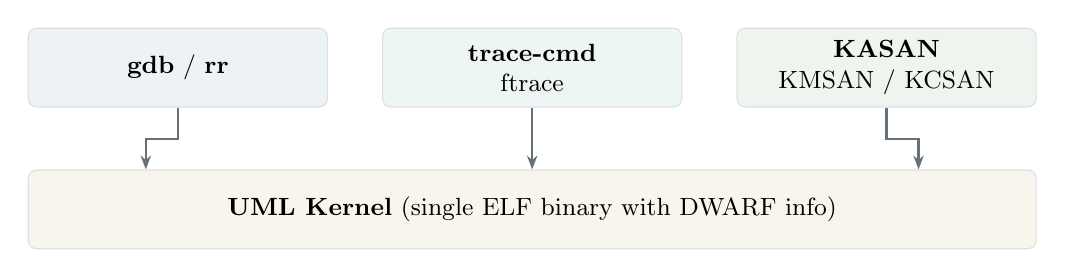
\begin{tikzpicture}[
    box/.style={
      draw=UMLGrid,
      fill=#1,
      minimum width=3.8cm,
      minimum height=1.0cm,
      rounded corners=3pt,
      font=\small,
      align=center
    },
    arrow/.style={
      -{Stealth[length=5pt]},
      thick,
      color=UMLMuted
    }
  ]

  % Developer tools
  \node[box=UMLBlue!8]  (gdb)    at (0,0)     {\textbf{gdb} / \textbf{rr}};
  \node[box=UMLTeal!8]  (trace)  at (4.5,0)   {\textbf{trace-cmd}\\ftrace};
  \node[box=UMLGreen!8] (san)    at (9,0)     {\textbf{KASAN}\\KMSAN / KCSAN};

  % UML kernel
  \node[box=KernelGold!8,minimum width=12.8cm] (uml) at (4.5,-1.8)
    {\textbf{UML Kernel} (single ELF binary with DWARF info)};

  % Arrows
  \draw[arrow] (gdb.south)   -- ++(0,-0.4) -| ($(uml.north west)+(1.5,0)$);
  \draw[arrow] (trace.south) -- (uml.north);
  \draw[arrow] (san.south)   -- ++(0,-0.4) -| ($(uml.north east)+(-1.5,0)$);

\end{tikzpicture}
\caption[Kernel debugging ecosystem under UML]{%
  Three complementary debugging approaches available when running the
  kernel under \UML{}: interactive debugging with \texttt{gdb} (or
  \texttt{rr} for record/replay), dynamic tracing with ftrace and
  \texttt{trace-cmd}, and compile-time sanitizers (KASAN, KMSAN, KCSAN).
  All three operate on the same kernel binary and can be used
  simultaneously.
}
\label{fig:app-debug-ecosystem}
\end{figure}


% ------------------------------------------------------------------
\section{Kernel Fuzzing}
\label{sec:app-fuzzing}
% ------------------------------------------------------------------

Coverage-guided kernel fuzzing is the most effective automated technique
for finding kernel bugs.  Google's syzkaller~\cite{syzkaller,vyukov2015}
is the world's most widely used kernel fuzzer, responsible for
discovering thousands of bugs in the Linux kernel since its introduction
in 2015.  Understanding how \UML{} fits into the fuzzing landscape
requires examining both the current state of the art and the
performance bottlenecks that limit it.

\subsection{The current landscape: QEMU-KVM}

Syzkaller's standard deployment targets QEMU/KVM virtual machines.
Each fuzzing instance boots a kernel inside a QEMU VM, runs a
\texttt{syz-executor} process that generates and executes syscall
programs, and collects coverage feedback via KCOV
(\texttt{CONFIG\_KCOV}).  The fuzzer mutates syscall sequences based
on which new code paths were exercised.

This architecture works well but imposes significant overhead:

\begin{enumerate}[leftmargin=2em]
  \item \textbf{Boot time.}  A QEMU/KVM instance takes 2--5 seconds to
        boot to the point where the fuzzer can begin executing syscalls.
  \item \textbf{Hardware requirement.}  QEMU/KVM requires
        \texttt{/dev/kvm}, which is unavailable in many CI/CD environments,
        nested virtualization scenarios, and shared cloud instances.
  \item \textbf{Communication overhead.}  The fuzzer communicates with
        the executor inside the VM through a virtio-serial channel or SSH.
        Each syscall program dispatch involves cross-VM communication.
  \item \textbf{Reset time.}  After a crash, the VM must be rebooted
        or restored from a snapshot, adding seconds of dead time.
\end{enumerate}

\subsection{The LKL precedent}

The Linux Kernel Library~\cite{lkl,purdila2010} demonstrated what
becomes possible when these overheads are eliminated.  By compiling the
kernel as a library and executing syscalls as function calls within the
same process, LKL-based fuzzers achieved approximately 60$\times$ the
throughput of QEMU-based approaches.  The LKL fuzzer can execute millions
of syscall sequences per second because there is no VM boundary, no boot
process, and no communication channel---the fuzzer and the kernel share
an address space.

However, LKL achieves this speed by sacrificing fidelity.  There is no
user/kernel separation, no process scheduling, no realistic signal
delivery, and no memory protection.  Bugs that depend on race conditions
between user and kernel execution, memory mapping semantics, or signal
handling are invisible to an LKL-based fuzzer.  The attack surface that
LKL exposes is a strict subset of the real kernel's attack surface.

\subsection{UML as a fuzzing target}

\UML{} occupies the sweet spot between QEMU and LKL:

\begin{table}[ht]
\centering
\caption{Fuzzing target comparison}
\label{tab:fuzz-comparison}
\begin{tabularx}{\textwidth}{l Y Y Y}
\toprule
\textbf{Property}  & \textbf{QEMU/KVM} & \textbf{LKL} & \textbf{UML (v2)} \\
\midrule
Boot time         & 2--5\,s           & N/A (library)    & $<$\,500\,ms \\
Syscall fidelity  & Full              & Partial          & Full \\
Process isolation & Full (HW)         & None             & Full (SW) \\
KCOV support      & Yes               & Custom           & Yes \\
Hardware requirement & /dev/kvm       & None             & None \\
Reset mechanism   & VM reboot/snapshot & Process restart & Snapshot/restore \\
Reset time        & 2--5\,s           & $<$\,1\,ms       & $<$\,1\,ms \\
\bottomrule
\end{tabularx}
\end{table}

With the v2 redesign's snapshot/restore capability, a \UML{} fuzzing
instance can be reset to a known-good state in under a millisecond.
The instance boots once, reaches the fuzzing entry point, takes a
snapshot, and then restores to that snapshot after each syscall sequence.
This eliminates boot time from the critical path entirely.

\subsection{The syzkaller vm/uml backend}

Syzkaller's architecture already supports pluggable VM backends through
its \texttt{vm/} package.  Adding a \UML{} backend requires implementing
the \texttt{vmimpl.Pool} and \texttt{vmimpl.Instance} interfaces:

\begin{itemize}[leftmargin=2em]
  \item \texttt{Create()} --- launch a \UML{} instance with the fuzzing
        kernel and root filesystem.
  \item \texttt{Forward()} --- set up port forwarding (trivial with \UML{}'s
        host networking).
  \item \texttt{Copy()} --- copy the \texttt{syz-executor} binary into the
        guest (via \texttt{hostfs}).
  \item \texttt{Run()} --- execute a command inside the guest and capture
        output.
  \item \texttt{Close()} --- terminate the instance.
\end{itemize}

Because \UML{} guest filesystems can be mounted via \texttt{hostfs}---a
direct pass-through of the host filesystem---there is no need for the
SSH or serial-port communication channels that QEMU requires.  The
fuzzer can write syscall programs directly to a shared directory and
read coverage data from the same path.

\subsection{KCOV integration}

KCOV (\texttt{CONFIG\_KCOV}) instruments the kernel to record which
basic blocks are executed during each syscall.  \UML{} supports KCOV
natively because KCOV is architecture-independent---it hooks into the
compiler's instrumentation callbacks, not into architecture-specific
trap handling.  The \texttt{/sys/kernel/debug/kcov} interface is
available inside the \UML{} guest and can be accessed through
\texttt{hostfs} from the host-side fuzzer.


% ------------------------------------------------------------------
\section{Network Simulation}
\label{sec:app-network}
% ------------------------------------------------------------------

One of the most successful real-world deployments of \UML{} has been
in network simulation and education, where the ability to run many
independent Linux instances---each with its own full networking
stack---without any hardware virtualization support has proven
invaluable.

\subsection{Netkit}

Netkit~\cite{pizzonia2008}, developed by Maurizio Pizzonia and Massimo
Rimondini at Roma Tre University, is the most widely used \UML{}-based
networking tool.  Each Netkit ``virtual machine'' is a \UML{} instance
connected to virtual Ethernet segments implemented as UNIX domain sockets.
A lab configuration file specifies the topology: which machines exist,
which interfaces they have, and which virtual collision domains they
connect to.

A typical Netkit lab might define a topology with:

\begin{itemize}[leftmargin=2em]
  \item Three routers running OSPF (via Quagga or FRRouting).
  \item Two Ethernet segments with multiple hosts.
  \item A NAT gateway connecting the virtual topology to the host network.
  \item A DNS server and a web server on separate subnets.
\end{itemize}

Each of these ``machines'' is a \UML{} process consuming 32--64\,MB of
memory.  A laptop can run dozens of instances simultaneously, enabling
students to build and experiment with network topologies that would
otherwise require a rack of physical hardware.

Netkit has been adopted by universities in Italy, Brazil, Germany,
Australia, and elsewhere for teaching courses on computer networking,
network security, and system administration.  The Netkit-NG fork
updated the project for modern kernels, and Kathara (a Docker-based
reimagining) continues the tradition, though with a shift away from
\UML{} toward containers.

\subsection{Marionnet}

Marionnet~\cite{marionnet}, developed at Paris 13 University, provides
a graphical interface for building virtual network topologies using
\UML{}.  Students drag and drop routers, switches, and hosts onto a
canvas, connect them with virtual cables, and then start the entire
topology.  Each node runs a full Linux instance under \UML{}, providing
realistic behavior including ARP, ICMP, TCP connection establishment,
and routing protocol convergence.

\subsection{Wireless network simulation}

Intel's WiFi team has used \UML{} for wireless network simulation,
running multiple \UML{} instances with virtual wireless interfaces
(mac80211\_hwsim) to test WiFi drivers and the \texttt{cfg80211}/\texttt{mac80211}
stack without physical wireless hardware.  This allows automated testing
of scenarios like roaming, channel switching, power management, and
multi-AP coordination that would be difficult to reproduce reliably
with physical hardware.

\begin{figure}[ht]
\centering
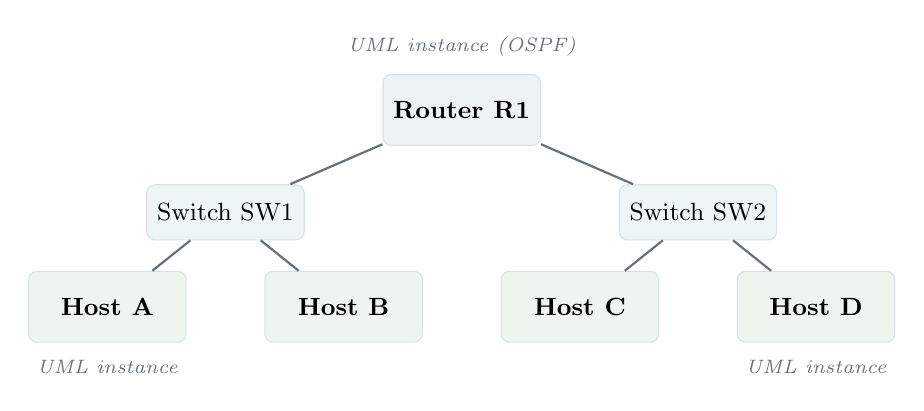
\begin{tikzpicture}[
    host/.style={
      draw=UMLGrid,
      fill=UMLGreen!8,
      minimum width=2.0cm,
      minimum height=0.9cm,
      rounded corners=3pt,
      font=\small\bfseries
    },
    switch/.style={
      draw=UMLGrid,
      fill=UMLTeal!8,
      minimum width=2.0cm,
      minimum height=0.7cm,
      rounded corners=3pt,
      font=\small
    },
    router/.style={
      draw=UMLGrid,
      fill=UMLBlue!8,
      minimum width=2.0cm,
      minimum height=0.9cm,
      rounded corners=3pt,
      font=\small\bfseries
    },
    link/.style={
      thick,
      color=UMLMuted
    }
  ]

  % Router
  \node[router] (r1) at (4.5,2.5) {Router R1};

  % Switches
  \node[switch] (sw1) at (1.5,1.2) {Switch SW1};
  \node[switch] (sw2) at (7.5,1.2) {Switch SW2};

  % Hosts
  \node[host] (h1) at (0,0) {Host A};
  \node[host] (h2) at (3,0) {Host B};
  \node[host] (h3) at (6,0) {Host C};
  \node[host] (h4) at (9,0) {Host D};

  % Links
  \draw[link] (r1) -- (sw1);
  \draw[link] (r1) -- (sw2);
  \draw[link] (sw1) -- (h1);
  \draw[link] (sw1) -- (h2);
  \draw[link] (sw2) -- (h3);
  \draw[link] (sw2) -- (h4);

  % Labels
  \node[font=\scriptsize\itshape,color=UMLMuted,below=0.1cm of h1]
    {UML instance};
  \node[font=\scriptsize\itshape,color=UMLMuted,below=0.1cm of h4]
    {UML instance};
  \node[font=\scriptsize\itshape,color=UMLMuted,above=0.1cm of r1]
    {UML instance (OSPF)};

\end{tikzpicture}
\caption[Netkit-style network topology]{%
  A simple Netkit-style network topology.  Each host, switch, and
  router is an independent \UML{} instance.  Virtual Ethernet
  segments are implemented as UNIX domain sockets on the host.
  The entire topology runs as ordinary userspace processes without
  any hardware virtualization.
}
\label{fig:app-netkit}
\end{figure}


% ------------------------------------------------------------------
\section{Security Research}
\label{sec:app-security}
% ------------------------------------------------------------------

Security researchers need environments where they can safely execute
kernel exploits, analyze malware behavior at the kernel level, and
develop mitigations---all without risking the host system.  \UML{}
provides this environment with properties that neither containers nor
traditional VMs fully match.

\subsection{Kernel exploit development and analysis}

When analyzing a kernel vulnerability---say, a use-after-free in a
filesystem driver---a researcher needs to:

\begin{enumerate}[leftmargin=2em]
  \item Build a kernel with the vulnerable code and full debug symbols.
  \item Trigger the vulnerability reliably.
  \item Observe the kernel state at the moment of corruption.
  \item Develop and test a mitigation.
\end{enumerate}

With \UML{}, every step happens in a single terminal session.  The
researcher builds the vulnerable kernel as an ELF binary, runs it
under \texttt{gdb}, sets a watchpoint on the freed memory region,
and observes the exact instruction that performs the use-after-free.
The kernel's full DWARF debug information is available, so the
researcher can inspect the call stack, the state of the slab
allocator, and the contents of every relevant data structure.

\subsection{Advantage over containers}

Containers (Docker, Kubernetes) share the host kernel.  A kernel
exploit that works in a container works against the host.  This is
not a theoretical concern: container escape vulnerabilities
(CVE-2019-5736, CVE-2020-15257, CVE-2022-0185) regularly demonstrate
that namespace and cgroup isolation do not constitute a security
boundary at the kernel level.

\UML{} provides genuine kernel isolation.  Each \UML{} instance
runs its own kernel in a separate address space.  A kernel exploit
that achieves code execution inside a \UML{} instance has compromised
a userspace process from the host's perspective.  It has no access
to the host kernel's data structures, no ability to manipulate host
page tables, and no path to privilege escalation on the host.  The
host kernel's normal process isolation guarantees contain the
compromised \UML{} instance.

\subsection{Honeypot deployment}

\UML{}'s lightweight footprint makes it practical to deploy
kernel-level honeypots.  Each honeypot is a \UML{} instance running
a deliberately vulnerable kernel, configured to log all system calls
and network traffic.  Because \UML{} instances are ordinary processes,
they can be monitored, resource-limited (via cgroups), and terminated
from the host without any special hypervisor tooling.  The host can
run dozens or hundreds of honeypot instances, each presenting a
different kernel version or configuration to probe for attacker
behavior.

\subsection{Malware analysis}

Kernel-level malware (rootkits, bootkits) requires a real kernel
environment for analysis.  Running such malware in a container is
dangerous because the malware has direct access to the host kernel.
Running it in a QEMU VM is safe but makes observation difficult:
the analyst must use the GDB remote protocol or custom QEMU plugins
to inspect kernel state.  \UML{} provides the best of both
worlds---a real kernel that the malware can infect, with the full
observability of a native userspace process.


% ------------------------------------------------------------------
\section{CI/CD and Automated Testing}
\label{sec:app-cicd}
% ------------------------------------------------------------------

Continuous integration and testing of kernel code requires an
environment that can boot a kernel, run tests, and report results.
The dominant approach uses QEMU/KVM, but this has a fundamental
limitation: it requires access to \texttt{/dev/kvm}.

\subsection{The /dev/kvm problem}

Many CI/CD environments lack hardware virtualization support:

\begin{description}[style=nextline,leftmargin=2em]
  \item[GitHub Actions (default runners).]
    The standard GitHub-hosted runners do not expose \texttt{/dev/kvm}.
    Larger runners with KVM access are available at increased cost.
  \item[Shared cloud instances.]
    Many cloud providers do not support nested virtualization on their
    standard instance types.  Even when nested virtualization is
    available, it incurs significant performance overhead.
  \item[Containerized CI.]
    CI systems that run jobs inside containers (Jenkins with Docker,
    GitLab CI) typically do not pass through \texttt{/dev/kvm} to
    the container for security reasons.
  \item[Locked-down workstations.]
    Corporate environments may disable hardware virtualization in BIOS
    or restrict access to \texttt{/dev/kvm} via udev rules.
\end{description}

\UML{} with the \Seccomp{} or \texttt{ptrace} backend has no such
requirement.  It runs wherever a Linux userspace process can run.
This makes it uniquely suited for kernel testing in environments where
hardware-assisted virtualization is unavailable.

\subsection{kselftest integration}

The kernel's self-test framework (\texttt{tools/testing/selftests/})
includes tests that require a running kernel environment.  The v2
redesign adds a comprehensive test suite under
\umlpath{tools/testing/selftests/um/} that exercises backend lifecycle
management, syscall interception, SMP behavior, and memory management.

These tests can be run as part of a standard CI pipeline:

\begin{lstlisting}[language=bash,caption={Running kselftest under UML in CI}]
# Build UML kernel with kselftest support
make ARCH=um O=build-um defconfig
make ARCH=um O=build-um -j$(nproc)

# Run the UML-specific selftests
make ARCH=um O=build-um -C tools/testing/selftests/um run_tests

# Run broader kernel selftests under UML
./build-um/vmlinux mem=512M \
    init=/path/to/run-selftests.sh
\end{lstlisting}

\subsection{Linux Test Project (LTP)}

The Linux Test Project (LTP) is a comprehensive test suite covering
syscall behavior, filesystem semantics, memory management, IPC, and
networking.  LTP tests can run inside a \UML{} instance with no
modifications, exercising the real kernel code paths.  Because \UML{}
boots in under a second, a CI pipeline can boot a fresh \UML{} instance
for each test group, providing isolation without the multi-second
overhead of QEMU boot cycles.

\subsection{Bisection workflows}

When a kernel regression is identified, \texttt{git bisect} requires
building and testing many kernel versions.  With QEMU, each test
iteration takes 10--30 seconds (build + boot + test + shutdown).
With \UML{}, the same cycle takes 2--5 seconds because:

\begin{enumerate}[leftmargin=2em]
  \item \UML{} builds are faster (smaller architecture-specific code).
  \item Boot time is under 500\,ms.
  \item No VM teardown is needed---the process simply exits.
\end{enumerate}

Over a typical bisection of 12--15 steps, this difference compounds
from minutes with QEMU to under a minute with \UML{}.


% ------------------------------------------------------------------
\section{Education}
\label{sec:app-education}
% ------------------------------------------------------------------

Operating systems courses have a persistent pedagogical problem: the
gap between theory and practice.  Students learn about schedulers,
virtual memory, and file systems in lecture, but interacting with a
real kernel traditionally required dedicated hardware, serial console
access, and the risk of bricking a machine.

\subsection{UML as a teaching tool}

\UML{} eliminates this barrier.  Every student can:

\begin{enumerate}[leftmargin=2em]
  \item Clone the kernel source tree on their laptop.
  \item Build it as a \texttt{ARCH=um} binary in minutes
        (faster than a full x86 build because the architecture-specific
        code is smaller).
  \item Run the kernel in a terminal window.
  \item Modify kernel code, rebuild, and re-run---a cycle measured in
        seconds.
  \item Attach \texttt{gdb} to observe the scheduler making decisions,
        the page fault handler allocating pages, or the VFS dispatching
        I/O to a filesystem.
\end{enumerate}

There is no risk to the student's laptop.  The worst that can happen
is the \UML{} process crashes---which is itself an educational
experience, as the student can examine the core dump.

\subsection{Concrete course applications}

\begin{description}[style=nextline,leftmargin=2em]
  \item[Process scheduling.]
    Students can add \texttt{printk} statements to the CFS scheduler,
    rebuild in seconds, and observe the scheduling decisions made for
    competing workloads.  With \texttt{gdb}, they can single-step
    through \texttt{pick\_next\_task\_fair()} and watch the red-black
    tree traversal in real time.

  \item[Virtual memory.]
    Students can trace page fault handling from the initial trap through
    \texttt{handle\_mm\_fault()}, page table walk, page allocation, and
    PTE installation.  \UML{}'s memory management uses host \syscall{mmap}
    calls, making it possible to correlate kernel-level page faults with
    host-level memory operations.

  \item[Filesystem implementation.]
    Students can build a minimal filesystem module, load it into a
    running \UML{} instance, and trace the complete path of a
    \syscall{read} call from the system call entry point through the
    VFS layer, the filesystem-specific \texttt{read\_iter} implementation,
    and the block layer.

  \item[Device drivers.]
    \UML{}'s virtual device model allows students to write simple
    character and block device drivers that interact with host-side
    files.  The driver runs in the \UML{} kernel, and its behavior
    can be observed from both the guest perspective (via
    \texttt{/dev/} entries) and the host perspective (via
    \texttt{gdb} and \texttt{strace}).

  \item[Concurrency and synchronization.]
    With SMP support in the v2 redesign, students can observe real
    lock contention, priority inversion, and RCU grace periods.  KCSAN
    can be enabled to catch data races, turning abstract concurrency
    bugs into concrete, reproducible reports.
\end{description}

\subsection{Comparison with teaching alternatives}

\begin{table}[ht]
\centering
\caption{Comparison of OS teaching environments}
\label{tab:edu-comparison}
\begin{tabularx}{\textwidth}{l Y Y Y Y}
\toprule
\textbf{Property} & \textbf{xv6} & \textbf{QEMU/KVM} & \textbf{Minix} & \textbf{UML} \\
\midrule
Real kernel code    & No   & Yes  & No   & Yes \\
Native debugging    & No   & GDB remote & No & GDB native \\
Rebuild cycle       & Fast & Slow & Medium & Fast \\
Hardware required   & None & /dev/kvm & None & None \\
Industry relevance  & Low  & High & Low  & High \\
\bottomrule
\end{tabularx}
\end{table}

xv6 (MIT's teaching OS) is elegant and well-documented, but it is
not Linux.  Skills learned in xv6 do not directly transfer to
kernel development.  QEMU/KVM runs real Linux but requires hardware
virtualization and imposes slow iteration cycles.  \UML{} is the
only option that combines the real Linux kernel with the fast
iteration and native debuggability that an educational environment
demands.


% ------------------------------------------------------------------
\section{Record/Replay for Bug Reproduction}
\label{sec:app-record-replay}
% ------------------------------------------------------------------

Many of the most difficult kernel bugs are non-deterministic: they
depend on the precise timing of interrupts, the order of concurrent
operations, or the exact sequence of I/O completions.  Reproducing
such bugs is often the hardest part of fixing them.  Record/replay
systems address this by capturing the non-deterministic inputs to a
computation during a ``record'' run and replaying them exactly during
a ``replay'' run, guaranteeing deterministic reproduction.

\subsection{Existing approaches}

\textbf{rr}~\cite{rr-project} (Mozilla) is the most successful
userspace record/replay system.  It records the results of system
calls, signal deliveries, and non-deterministic instructions
(\texttt{RDTSC}, \texttt{RDRAND}) during a recording session, and
replays them faithfully.  However, rr operates at the userspace level:
it can record and replay a userspace program, but it cannot record and
replay kernel execution.  If a bug is in the kernel, rr cannot help.

\textbf{ReVirt}~\cite{dunlap2002} demonstrated virtual machine-level
record/replay by logging all non-deterministic events (interrupts,
DMA, device I/O) entering a VM.  But ReVirt required modifications
to the hypervisor and imposed significant overhead.

\subsection{UML record/replay}

\UML{}'s architecture makes record/replay uniquely tractable.  The
sources of non-determinism in a \UML{} instance are precisely
enumerable:

\begin{enumerate}[leftmargin=2em]
  \item \textbf{Timer interrupts.}  Generated by host-side
        \texttt{SIGALRM} signals.  The record layer logs the exact
        instruction pointer at which each signal was delivered.
  \item \textbf{I/O completions.}  Disk reads, network packet arrivals,
        and other I/O events arrive as host system call return values.
        The record layer logs these values.
  \item \textbf{Inter-processor interrupts.}  In SMP mode, IPIs from
        other virtual CPUs introduce ordering non-determinism.  The
        record layer logs the IPI delivery order.
  \item \textbf{Host entropy.}  Calls to \syscall{getrandom} or reads
        from \texttt{/dev/urandom} on the host.  The record layer logs
        the returned bytes.
\end{enumerate}

During replay, the record layer intercepts each of these sources and
injects the logged values at the exact same points in execution.  The
result is bit-for-bit deterministic replay of the kernel's execution,
including all scheduler decisions, lock acquisitions, and memory
allocations.

\subsection{Time-travel debugging}

When combined with \texttt{gdb}, record/replay enables \emph{time-travel
debugging}: the ability to run the kernel execution backward.  The
developer can set a watchpoint on a corrupted data structure, run
backward to the point of corruption, and identify the exact code path
that caused it.  This is the kernel-level equivalent of rr's
\texttt{reverse-continue} command, applied to the kernel itself.

Jeff Dike implemented an early version of time-travel support for
\UML{}, and the v2 redesign extends this with SMP-aware recording
and the ability to replay across snapshot/restore boundaries.


% ------------------------------------------------------------------
\section{Snapshot/Restore for Fast Iteration}
\label{sec:app-snapshot}
% ------------------------------------------------------------------

The ability to capture the complete state of a running kernel and
restore it later is valuable for several workflows:

\subsection{Fuzzing reset}

As discussed in Section~\ref{sec:app-fuzzing}, coverage-guided fuzzers
need to reset the kernel to a clean state after each test iteration.
With snapshot/restore, this reset is a memory operation rather than a
reboot.  The v2 implementation captures:

\begin{itemize}[leftmargin=2em]
  \item All guest physical memory pages (via \syscall{mmap} snapshots).
  \item CPU register state for all virtual CPUs.
  \item Kernel timer state.
  \item Virtual device state (block device positions, network queue
        contents).
\end{itemize}

Restore replays these snapshots by remapping memory regions and
restoring register state.  Because \UML{}'s memory is ordinary
process memory (anonymous \syscall{mmap} regions), the snapshot can
use copy-on-write semantics: the restore operation marks all pages
as CoW, and only pages that are actually modified during the next
test iteration incur a copy.  This makes restore effectively
sub-microsecond for the common case where only a small fraction of
pages are modified between iterations.

\subsection{Debugging iteration}

A developer investigating a complex kernel bug can take a snapshot
just before the bug manifests, then repeatedly restore and re-examine
the bug with different breakpoints, watchpoints, or instrumentation.
This is similar to recording and replaying, but more flexible: the
developer can modify kernel code between restore iterations, recompile
individual modules, and reload them into the restored kernel.

\subsection{Test parallelization}

A single snapshot can be restored into multiple independent \UML{}
instances, each running a different test.  This enables embarrassingly
parallel testing: boot the kernel once, take a snapshot at the
test-ready state, and fork it into $N$ copies, each running one test
suite.  The boot cost is amortized across all test suites.

\begin{figure}[ht]
\centering
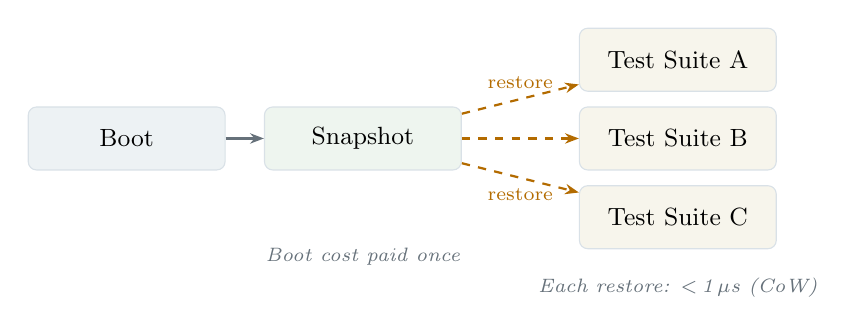
\begin{tikzpicture}[
    state/.style={
      draw=UMLGrid,
      fill=#1,
      minimum width=2.5cm,
      minimum height=0.8cm,
      rounded corners=3pt,
      font=\small
    },
    arrow/.style={
      -{Stealth[length=5pt]},
      thick,
      color=UMLMuted
    },
    darrow/.style={
      -{Stealth[length=5pt]},
      thick,
      dashed,
      color=UMLAmber
    }
  ]

  % Boot sequence
  \node[state=UMLBlue!8]  (boot)  at (0,0)     {Boot};
  \node[state=UMLGreen!8] (snap)  at (3,0)     {Snapshot};

  % Fork into multiple instances
  \node[state=KernelGold!8] (t1) at (7,1)   {Test Suite A};
  \node[state=KernelGold!8] (t2) at (7,0)   {Test Suite B};
  \node[state=KernelGold!8] (t3) at (7,-1)  {Test Suite C};

  % Restore arrows
  \draw[arrow] (boot) -- (snap);
  \draw[darrow] (snap) -- (t1) node[midway,above,font=\scriptsize] {restore};
  \draw[darrow] (snap) -- (t2);
  \draw[darrow] (snap) -- (t3) node[midway,below,font=\scriptsize] {restore};

  % Annotation
  \node[font=\scriptsize\itshape,color=UMLMuted] at (3,-1.5)
    {Boot cost paid once};
  \node[font=\scriptsize\itshape,color=UMLMuted] at (7,-1.9)
    {Each restore: $<$\,1\,$\mu$s (CoW)};

\end{tikzpicture}
\caption[Snapshot-based test parallelization]{%
  Snapshot-based test parallelization.  The kernel boots once and
  reaches a test-ready state.  A snapshot is taken and restored into
  multiple independent instances, each running a different test suite.
  Restore uses copy-on-write semantics for sub-microsecond latency.
}
\label{fig:app-snapshot-parallel}
\end{figure}


% ------------------------------------------------------------------
\section{Summary}
\label{sec:app-summary}
% ------------------------------------------------------------------

The applications surveyed in this chapter share a common theme:
\UML{} provides capabilities that require the \emph{combination} of
kernel fidelity, process-level debuggability, and minimal host
requirements---a combination that no other single technology offers.

\begin{table}[ht]
\centering
\caption{Application domains and key UML advantages}
\label{tab:app-summary}
\begin{tabularx}{\textwidth}{l Y Y}
\toprule
\textbf{Application} & \textbf{Key UML advantage} & \textbf{Alternative limitations} \\
\midrule
Kernel debugging   & Native gdb, full DWARF        & QEMU: remote protocol only \\
Kernel fuzzing     & No /dev/kvm, fast reset        & QEMU: slow boot; LKL: no isolation \\
Network simulation & Many instances, no HW virt     & Physical hardware: expensive \\
Security research  & Full kernel isolation           & Containers: shared kernel \\
CI/CD testing      & Runs anywhere Linux runs        & QEMU: requires /dev/kvm \\
Education          & Fast rebuild, native debug      & xv6: not real Linux \\
Record/replay      & Enumerable non-determinism      & rr: userspace only \\
Snapshot/restore   & Sub-$\mu$s CoW restore          & QEMU: multi-second restore \\
\bottomrule
\end{tabularx}
\end{table}

The v2 redesign strengthens \UML{}'s position in each of these domains.
The backend-ops abstraction allows choosing the optimal backend for each
use case (seccomp for portability, kvm-v2 for performance).  SMP support
enables testing of concurrent code paths.  Snapshot/restore and
record/replay transform \UML{} from a development convenience into a
serious research infrastructure.

Chapter~\ref{ch:related} examines how \UML{} compares to the related
systems that serve some of these same domains.

% ==========================================================================
%  Chapter 8 — Related Work and Comparative Analysis
% ==========================================================================
\chapter{Related Work}
\label{ch:related}

\epigraph{%
  Every isolation technology is a point in a multi-dimensional
  trade-off space: compatibility, performance, security, and
  operational complexity.  Understanding where each point lies is
  prerequisite to choosing wisely.%
}{}

User-Mode Linux does not exist in isolation.  The past two decades have
produced a rich ecosystem of virtualization, sandboxing, and kernel
abstraction technologies, each occupying a different point in the
design space.  This chapter provides a detailed comparison with nine
related systems, analyzing the architectural decisions that differentiate
them from \UML{} and the trade-offs those decisions entail.  We conclude
with a comprehensive comparison table (Section~\ref{sec:related-table})
that summarizes the landscape.

For each system, we describe the core architecture, identify the key
design decisions that differentiate it from \UML{}, and assess the
implications for compatibility, performance, security, and operational
deployment.


% ------------------------------------------------------------------
\section{gVisor}
\label{sec:related-gvisor}
% ------------------------------------------------------------------

\subsection{Architecture}

gVisor~\cite{gvisor} is Google's user-space kernel, open-sourced in
2018.  Its core component, the \emph{Sentry}, is a process written
in Go that reimplements approximately 200 Linux system calls.  When
a containerized application issues a system call, it is intercepted
and handled by the Sentry rather than by the host Linux kernel.  This
interposition provides a security boundary: even if the application
exploits a bug in the Sentry's syscall implementation, it cannot
directly compromise the host kernel.

gVisor has evolved through three platform backends~\cite{gvisor-platforms}:

\begin{description}[style=nextline,leftmargin=2em]
  \item[ptrace (2018).]
    The original platform.  The Sentry attaches to application
    processes via \texttt{ptrace} and intercepts syscalls.  This is
    architecturally identical to \UML{}'s original mechanism, and it
    suffers from the same performance limitations: each syscall
    requires multiple context switches between the tracer (Sentry)
    and the tracee (application).

  \item[KVM (2018).]
    The Sentry runs in a lightweight KVM virtual machine.
    Application code runs in guest ring 3; the Sentry runs in guest
    ring 0.  Syscall traps are handled as VM exits.  This is
    conceptually similar to \UML{}'s \KVMvTwo{} backend, but the
    ``kernel'' being run in ring 0 is the Go Sentry, not the real
    Linux kernel.

  \item[Systrap (2023).]
    The newest platform~\cite{gvisor-systrap}.  It uses a combination
    of shared memory, per-thread signal handlers, and a dedicated
    ``stub'' process to handle syscalls without the overhead of
    \texttt{ptrace} or \KVM{}.  The application's syscall instruction
    triggers a \texttt{SIGSYS} signal (installed via seccomp-BPF),
    which vectors to a handler that dispatches the syscall to the
    Sentry via shared memory.  This achieves near-native performance
    for many workloads.
\end{description}

\subsection{Key difference: reimplementation vs.\ the real kernel}

The fundamental architectural difference between gVisor and \UML{}
is that gVisor \emph{reimplements} the Linux syscall interface while
\UML{} \emph{is} the Linux kernel.  This distinction has profound
consequences:

\begin{description}[style=nextline,leftmargin=2em]
  \item[Compatibility.]
    gVisor's Sentry implements a subset of the Linux ABI.  System
    calls that are not implemented, or whose semantics differ subtly
    from the kernel's implementation, can cause application failures.
    Google maintains a compatibility matrix documenting which syscalls
    are supported and at what level of fidelity.  \UML{}, by contrast,
    supports every syscall that the Linux kernel supports, because it
    \emph{is} the Linux kernel.  There is no compatibility matrix
    because there is no reimplementation.

  \item[Bug fidelity.]
    A bug found in gVisor is a bug in the Go Sentry code.  It may or
    may not correspond to a real kernel bug.  A bug found in \UML{}
    is a bug in the Linux kernel source tree, directly applicable to
    every architecture.  This makes \UML{} suitable for kernel
    development and testing in a way that gVisor fundamentally is not.

  \item[Security posture.]
    gVisor's reimplementation is a \emph{feature} from a security
    perspective: by not running the real kernel, it avoids exposing
    the real kernel's attack surface to untrusted containers.  The
    Sentry presents a smaller, memory-safe (Go) attack surface.
    \UML{}, running the real kernel, inherits the real kernel's
    vulnerabilities.  However, those vulnerabilities are contained
    within a host-level process, so exploitation achieves
    compromise of a userspace process, not the host kernel.
\end{description}

\subsection{Performance comparison}

gVisor with the systrap platform achieves syscall latencies of
approximately 1--3\,$\mu$s for simple syscalls~\cite{gvisor-systrap}.
\UML{} with the \Seccomp{} backend achieves approximately 300\,ns;
with \KVMvTwo{}, approximately 100\,ns.  For I/O-intensive workloads,
gVisor's overhead is dominated by the cost of reimplementing filesystem
and networking operations in Go, whereas \UML{} uses the kernel's
native C implementations.  For compute-intensive workloads where
syscalls are infrequent, both systems approach native performance.

\begin{figure}[ht]
\centering
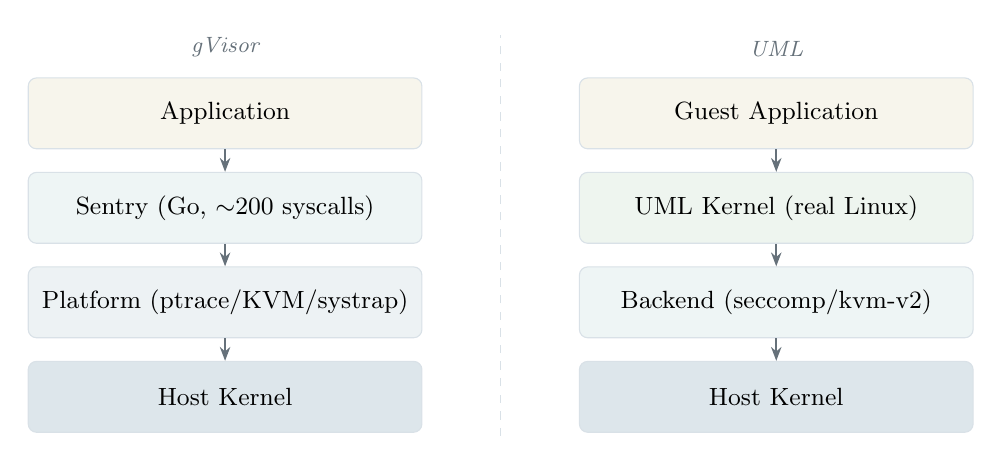
\begin{tikzpicture}[
    layer/.style={
      draw=UMLGrid,
      fill=#1,
      minimum width=5cm,
      minimum height=0.9cm,
      rounded corners=3pt,
      font=\small,
      align=center
    },
    label/.style={
      font=\footnotesize\itshape,
      color=UMLMuted,
      anchor=south
    },
    arrow/.style={
      -{Stealth[length=5pt]},
      thick,
      color=UMLMuted
    }
  ]

  % gVisor stack (left)
  \node[label] at (-3.5,4.6) {gVisor};
  \node[layer=KernelGold!8] (gapp) at (-3.5,4)  {Application};
  \node[layer=UMLTeal!8]    (gsen) at (-3.5,2.8) {Sentry (Go, $\sim$200 syscalls)};
  \node[layer=UMLBlue!8]    (gplat) at (-3.5,1.6) {Platform (ptrace/KVM/systrap)};
  \node[layer=UMLBlue!15]   (ghost) at (-3.5,0.4) {Host Kernel};

  \draw[arrow] (gapp.south) -- (gsen.north);
  \draw[arrow] (gsen.south) -- (gplat.north);
  \draw[arrow] (gplat.south) -- (ghost.north);

  % UML stack (right)
  \node[label] at (3.5,4.6) {UML};
  \node[layer=KernelGold!8] (uapp) at (3.5,4)  {Guest Application};
  \node[layer=UMLGreen!8]   (uker) at (3.5,2.8) {UML Kernel (real Linux)};
  \node[layer=UMLTeal!8]    (ubak) at (3.5,1.6) {Backend (seccomp/kvm-v2)};
  \node[layer=UMLBlue!15]   (uhost) at (3.5,0.4) {Host Kernel};

  \draw[arrow] (uapp.south) -- (uker.north);
  \draw[arrow] (uker.south) -- (ubak.north);
  \draw[arrow] (ubak.south) -- (uhost.north);

  % Separator
  \draw[dashed,color=UMLGrid] (0,-0.1) -- (0,5.0);

\end{tikzpicture}
\caption[gVisor vs.\ UML architecture]{%
  Architectural comparison of gVisor and \UML{}.  gVisor interposes a
  Go-language Sentry that reimplements Linux syscalls.  \UML{} runs the
  actual Linux kernel, using a backend for syscall interception.  The
  layers are analogous but the kernel layer is fundamentally different:
  reimplementation (gVisor) vs.\ the real kernel (\UML{}).
}
\label{fig:related-gvisor-uml}
\end{figure}


% ------------------------------------------------------------------
\section{Firecracker}
\label{sec:related-firecracker}
% ------------------------------------------------------------------

\subsection{Architecture}

Firecracker~\cite{agache2020,firecracker} is a virtual machine monitor
(VMM) developed by Amazon Web Services (AWS) and open-sourced in 2018.
Written in Rust, it uses the KVM API to create lightweight virtual
machines (``microVMs'') with a minimal device model.  Firecracker is
the execution engine behind AWS Lambda and AWS Fargate.

A Firecracker microVM includes:

\begin{itemize}[leftmargin=2em]
  \item A KVM-based virtual CPU with full hardware-assisted
        virtualization (Intel VT-x / AMD-V).
  \item A minimal device model: virtio-net, virtio-block, a serial
        console, and a minimal i8042 keyboard controller.  No PCI bus,
        no USB, no GPU emulation.
  \item A custom boot protocol that loads the guest kernel directly
        into memory, bypassing BIOS/UEFI boot.
\end{itemize}

Firecracker achieves cold-start times of under 125\,ms and memory
overhead of approximately 5\,MB per microVM.

\subsection{Key difference: full VM vs.\ process}

Firecracker runs a \emph{complete virtual machine} with its own kernel
instance, guest physical memory, and emulated hardware.  The guest kernel
runs in the VM's ring 0 (guest mode), with full hardware privilege within
the VM.  Communication between the guest and the host occurs through
virtio devices and VM exits.

\UML{} runs the kernel as a \emph{process}.  There is no emulated hardware,
no virtio devices (in the conventional sense), and no guest physical memory
separate from the host's process address space.  The \UML{} kernel
accesses host resources through system calls, not through device emulation.

\begin{description}[style=nextline,leftmargin=2em]
  \item[Isolation model.]
    Firecracker provides hardware-enforced isolation: the guest cannot
    access host memory outside its designated physical memory region
    because the CPU's EPT/NPT page tables prevent it.  \UML{} provides
    software-enforced isolation: the guest cannot access host memory
    because the host kernel's process isolation prevents it.  Both
    provide strong isolation, but Firecracker's hardware enforcement
    is a stronger guarantee against kernel vulnerabilities in the host.

  \item[Use case.]
    Firecracker is designed for multi-tenant cloud isolation: running
    thousands of untrusted customer workloads on shared hardware.
    \UML{} is designed for kernel development, debugging, testing,
    and research---environments where the guest is not necessarily
    untrusted, but where observability and fast iteration matter more
    than multi-tenant security.

  \item[Hardware requirements.]
    Firecracker requires \texttt{/dev/kvm} and hardware virtualization
    extensions.  \UML{} with the \Seccomp{} or \texttt{ptrace} backend
    requires neither.

  \item[Host tool access.]
    A Firecracker guest is an opaque VM from the host's perspective.
    Debugging the guest kernel requires GDB remote protocol over serial.
    A \UML{} guest is a host process: \texttt{gdb}, \texttt{strace},
    \texttt{perf}, and every other host tool work directly.
\end{description}

\subsection{Performance}

For I/O throughput, Firecracker benefits from virtio's efficient
batched I/O model and KVM's hardware-accelerated instruction
execution.  For syscall-heavy workloads, the VM exit cost
(approximately 1--2\,$\mu$s per exit on modern hardware) is
comparable to \UML{}'s \Seccomp{} backend.  \UML{}'s \KVMvTwo{}
backend, which also uses KVM but avoids the full VM device model,
can achieve lower per-syscall latency because the exit handler is a
simple function call within the \UML{} process, not a return to
a separate VMM process.


% ------------------------------------------------------------------
\section{Linux Kernel Library (LKL)}
\label{sec:related-lkl}
% ------------------------------------------------------------------

\subsection{Architecture}

The Linux Kernel Library (\textsc{LKL})~\cite{purdila2010,lkl}
compiles the Linux kernel as a static library (\texttt{liblinux.a})
that can be linked into an ordinary application.  The application
calls kernel functions directly---\texttt{lkl\_sys\_open()},
\texttt{lkl\_sys\_read()}, etc.---and the kernel executes in the
same address space and at the same privilege level as the application.

\textsc{LKL} achieves this by:

\begin{enumerate}[leftmargin=2em]
  \item Implementing a minimal \texttt{arch/lkl/} port that maps
        kernel threading to host pthreads, kernel memory allocation
        to host \syscall{malloc}, and kernel timers to host timer
        APIs.
  \item Disabling the MMU.  There is no virtual memory translation;
        kernel and application share a flat address space.
  \item Disabling process scheduling.  There is no userspace; the
        kernel exists solely to provide its subsystems (VFS, networking,
        block layer) as library functions.
\end{enumerate}

\subsection{Performance}

\textsc{LKL}'s in-process execution model eliminates all
interposition overhead.  A ``syscall'' is a function call: the
application pushes arguments onto the stack, calls the kernel
function, and gets the result back immediately.  There is no context
switch, no signal delivery, no trap handler.  This makes \textsc{LKL}
extraordinarily fast for workloads that consist primarily of kernel
operations.

Fuzzing studies have reported approximately 60$\times$ throughput
improvement when using \textsc{LKL} compared to QEMU/KVM targets.
This number is the motivation for many of the v2 redesign's
performance optimizations.

\subsection{Limitations}

\textsc{LKL}'s speed comes at a fundamental cost:

\begin{description}[style=nextline,leftmargin=2em]
  \item[No user/kernel separation.]
    The application and the kernel share an address space.  A buffer
    overflow in the kernel can corrupt application data and vice versa.
    There is no protection boundary, so \textsc{LKL} cannot be used to
    study real syscall behavior where \syscall{copy\_from\_user} /
    \syscall{copy\_to\_user} semantics matter.

  \item[No process model.]
    \textsc{LKL} does not support multiple processes, scheduling, or
    signals.  Bugs that depend on process interaction, scheduling
    decisions, or signal delivery are invisible.

  \item[No SMP.]
    \textsc{LKL} is single-threaded from the kernel's perspective.
    Concurrency bugs, which are among the most dangerous kernel bugs,
    cannot be found or reproduced.

  \item[No realistic attack surface.]
    Because there is no user/kernel boundary, the attack surface that
    \textsc{LKL} exposes to a fuzzer is a strict subset of the real
    kernel's attack surface.  Entire classes of vulnerabilities---those
    involving user-pointer validation, memory mapping semantics, and
    inter-process communication---are absent.
\end{description}

\subsection{The LKL--UML unification effort}

Hajime Tazaki proposed unifying \textsc{LKL} into \UML{} in a series
of RFC patches~\cite{tazaki2019} that reached v8 before stalling.
The core idea was to make \textsc{LKL} a ``backend'' or operating
mode of \UML{}, sharing the same \texttt{arch/um/} code but with a
compilation option that strips away process isolation for maximum
speed.  This would allow a single codebase to serve both the
high-fidelity (\UML{}) and high-speed (\textsc{LKL}) use cases.

The v2 redesign's backend-ops abstraction lays the groundwork for
this unification.  A hypothetical \texttt{lkl} backend could implement
the \texttt{struct um\_backend\_ops} interface with trivial stubs
(no-op for process creation, direct function call for syscall
dispatch), providing \textsc{LKL}-like performance within the \UML{}
framework.

\begin{figure}[ht]
\centering
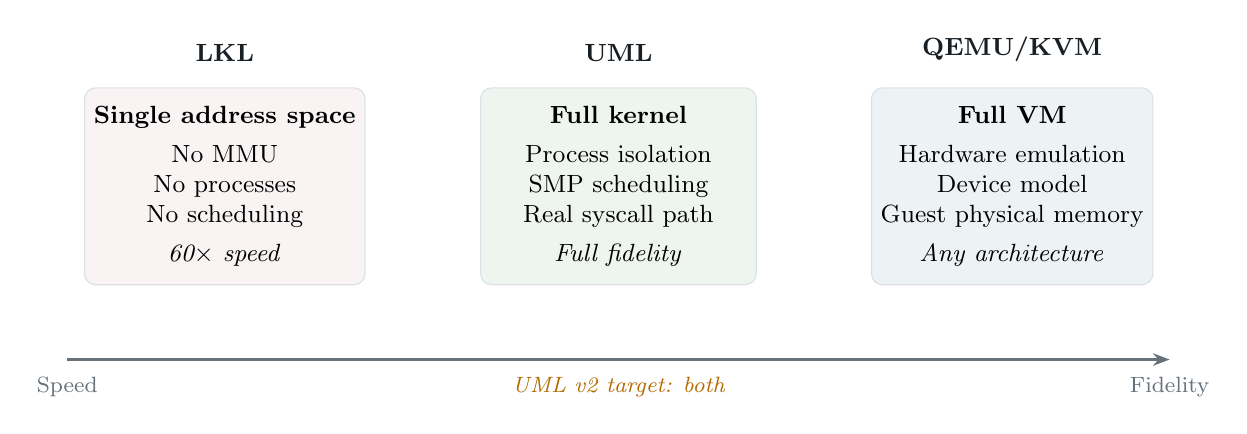
\begin{tikzpicture}[
    box/.style={
      draw=UMLGrid,
      fill=#1,
      minimum width=3.5cm,
      minimum height=2.5cm,
      rounded corners=4pt,
      font=\small,
      align=center
    },
    label/.style={
      font=\small\bfseries,
      color=UMLInk
    }
  ]

  % LKL
  \node[box=UMLRed!6] (lkl) at (0,0) {
    \textbf{Single address space}\\[3pt]
    No MMU\\
    No processes\\
    No scheduling\\[3pt]
    \textit{60$\times$ speed}
  };
  \node[label,above=0.2cm of lkl] {LKL};

  % UML
  \node[box=UMLGreen!8] (uml) at (5,0) {
    \textbf{Full kernel}\\[3pt]
    Process isolation\\
    SMP scheduling\\
    Real syscall path\\[3pt]
    \textit{Full fidelity}
  };
  \node[label,above=0.2cm of uml] {UML};

  % QEMU
  \node[box=UMLBlue!8] (qemu) at (10,0) {
    \textbf{Full VM}\\[3pt]
    Hardware emulation\\
    Device model\\
    Guest physical memory\\[3pt]
    \textit{Any architecture}
  };
  \node[label,above=0.2cm of qemu] {QEMU/KVM};

  % Spectrum arrow
  \draw[-{Stealth[length=6pt]},very thick,color=UMLMuted]
    (-2,-2.2) -- (12,-2.2);
  \node[font=\footnotesize,color=UMLMuted,anchor=north] at (-2,-2.3)
    {Speed};
  \node[font=\footnotesize,color=UMLMuted,anchor=north] at (12,-2.3)
    {Fidelity};
  \node[font=\footnotesize\itshape,color=UMLAmber,anchor=north] at (5,-2.3)
    {UML v2 target: both};

\end{tikzpicture}
\caption[Speed--fidelity spectrum]{%
  The speed--fidelity spectrum of kernel execution environments.
  \textsc{LKL} maximizes speed by eliminating all isolation.
  QEMU/KVM maximizes fidelity by emulating complete hardware.
  \UML{} v2 aims to approach \textsc{LKL}'s speed while
  retaining full kernel fidelity.
}
\label{fig:related-spectrum}
\end{figure}


% ------------------------------------------------------------------
\section{QEMU and KVM}
\label{sec:related-qemu-kvm}
% ------------------------------------------------------------------

\subsection{Architecture}

QEMU~\cite{bellard2005} is a full-system emulator that translates
guest instructions to host instructions via a technique called
Tiny Code Generator (TCG) dynamic binary translation.  When combined
with KVM~\cite{kivity2007}, QEMU uses hardware virtualization
extensions to execute guest code directly on the CPU, with the TCG
path used only for emulating devices and handling privileged
instructions.

QEMU/KVM is the standard tool for kernel development and testing.
It provides:

\begin{itemize}[leftmargin=2em]
  \item Full hardware emulation: PCI bus, USB, network interfaces,
        block devices, GPU (via virtio-gpu or QXL), serial ports,
        RTC, APIC, IOAPIC, and more.
  \item Multi-architecture support: x86, ARM, RISC-V, PowerPC,
        MIPS, s390x, and others.
  \item Snapshot support via QEMU savevm.
  \item GDB debugging via the GDB remote protocol.
  \item Live migration between hosts.
\end{itemize}

\subsection{Comparison with UML}

\begin{description}[style=nextline,leftmargin=2em]
  \item[Architecture support.]
    QEMU can emulate any supported architecture on any host.  A
    developer can test an ARM kernel on an x86 workstation.  \UML{}
    runs only the host's native architecture (x86-64 on an x86-64
    host).  For cross-architecture testing, QEMU is the only option.

  \item[Device emulation.]
    QEMU provides realistic device emulation, essential for testing
    device drivers.  \UML{}'s devices are virtual abstractions
    (\texttt{ubd} for block, \texttt{tuntap}/\texttt{vector} for
    networking) that do not correspond to real hardware.  For driver
    development, QEMU is necessary.

  \item[Startup time.]
    QEMU/KVM requires 2--5 seconds to boot a kernel to userspace.
    \UML{} boots in under 500\,ms.  For workflows that require many
    boot cycles (bisection, fuzzing, CI), this difference is
    significant.

  \item[Debugging experience.]
    QEMU exposes a GDB remote protocol server.  The developer connects
    \texttt{gdb} to this server and debugs the guest kernel over a
    socket.  This works but imposes limitations: conditional breakpoints
    are evaluated on the debugger side (requiring round-trips for each
    check), variable inspection requires translating through guest page
    tables, and the full \texttt{gdb} Python scripting API is
    available but slow.

    \UML{} provides native \texttt{gdb} access.  The kernel is a
    local process; \texttt{gdb} reads its memory directly.  Conditional
    breakpoints evaluate at native speed.  The debugging experience
    is qualitatively superior.

  \item[Host tool access.]
    A QEMU guest is isolated from the host.  Sharing files requires
    virtio-9p, NFS, or SSH.  \texttt{strace}, \texttt{perf}, and
    other host tools cannot observe the guest kernel.  A \UML{} guest
    is a host process: all host tools work directly, and
    \texttt{hostfs} provides zero-overhead filesystem sharing.

  \item[Hardware requirements.]
    QEMU with TCG (software emulation) requires no hardware
    virtualization, but is 10--100$\times$ slower than native execution.
    QEMU/KVM requires \texttt{/dev/kvm}.  \UML{} with \Seccomp{}
    runs at near-native speed without any hardware requirements.
\end{description}

\subsection{Complementary roles}

\UML{} and QEMU/KVM are not competitors; they serve different
purposes.  QEMU/KVM is essential for cross-architecture testing,
driver development, and production virtualization.  \UML{} is
superior for kernel debugging, rapid iteration, and environments
lacking \texttt{/dev/kvm}.  A comprehensive kernel development
workflow uses both.


% ------------------------------------------------------------------
\section{Containers}
\label{sec:related-containers}
% ------------------------------------------------------------------

\subsection{Architecture}

Linux containers (Docker, Kubernetes, LXC) use namespaces and
cgroups~\cite{soltesz2007,namespaces,cgroups-v2} to provide
isolated execution environments that share the host kernel.  Each
container has its own view of the PID namespace, network namespace,
mount namespace, and (optionally) user namespace, but all containers
execute system calls against the same kernel instance.

Containers are extraordinarily lightweight---startup times of tens
of milliseconds, memory overhead of kilobytes---because there is
no kernel to boot, no device model to initialize, and no memory
to dedicate to a separate kernel instance.

\subsection{The shared-kernel problem}

The shared kernel is both containers' greatest strength and their
greatest weakness:

\begin{description}[style=nextline,leftmargin=2em]
  \item[Strength.]
    Because all containers share the kernel, there is no duplication
    of kernel memory, no boot overhead, and no performance penalty for
    syscall dispatch.  A containerized application's \syscall{read}
    call goes directly to the kernel with zero interposition overhead.

  \item[Weakness.]
    A kernel vulnerability is a vulnerability in \emph{every}
    container on the host.  Container escape exploits
    (CVE-2019-5736: runc; CVE-2020-15257: containerd; CVE-2022-0185:
    filesystem) demonstrate repeatedly that namespace and cgroup
    isolation do not constitute a security boundary.  The kernel
    developers explicitly document that namespaces are not a
    security feature for untrusted code.
\end{description}

\subsection{Comparison with UML}

\UML{} provides per-instance kernel isolation.  Each \UML{} instance
runs its own kernel, so a kernel vulnerability in one instance cannot
affect another instance or the host.  This comes at a cost:

\begin{itemize}[leftmargin=2em]
  \item \UML{} instances consume more memory (kernel per instance).
  \item \UML{} instances have longer startup times (kernel boot).
  \item Syscalls in \UML{} incur interposition overhead.
\end{itemize}

For multi-tenant isolation of untrusted workloads, the industry
has moved toward combining containers with lightweight VMs
(Firecracker, Kata Containers) or user-space kernels (gVisor).
\UML{} occupies a middle ground: lighter than a full VM, heavier
than a container, but with genuine kernel isolation and the unique
advantage of running the real kernel for development and testing
purposes.


% ------------------------------------------------------------------
\section{Unikernels}
\label{sec:related-unikernels}
% ------------------------------------------------------------------

\subsection{Architecture}

Unikernels~\cite{madhavapeddy2013,kuenzer2021} are specialized,
single-purpose machine images that combine an application with the
minimal set of kernel libraries needed to run it.  The application
and kernel run in a single address space at a single privilege level,
eliminating the user/kernel boundary.

Notable unikernel projects include:

\begin{description}[style=nextline,leftmargin=2em]
  \item[MirageOS~\cite{madhavapeddy2013}.]
    Written in OCaml.  Compiles an application and its OS dependencies
    into a single Xen or KVM bootable image.  Extremely small attack
    surface (no shell, no multi-user system, no unnecessary drivers).

  \item[Unikraft~\cite{kuenzer2021}.]
    A modular unikernel construction toolkit.  The developer selects
    which kernel components (scheduler, memory allocator, network
    stack) to include.  Achieves boot times under 1\,ms for minimal
    configurations and throughput exceeding that of Linux for
    specialized workloads.

  \item[IncludeOS.]
    A C++ unikernel for cloud applications.  The application
    \texttt{\#include}s the OS as a library.
\end{description}

\subsection{Comparison with UML}

\begin{description}[style=nextline,leftmargin=2em]
  \item[Boot time.]
    Unikernels boot in milliseconds (sometimes sub-millisecond for
    Unikraft), compared to \UML{}'s $\sim$500\,ms.  However,
    unikernels typically run on a hypervisor (Xen or KVM), so the
    total startup includes hypervisor overhead.

  \item[Compatibility.]
    Unikernels sacrifice compatibility for specialization.  A
    MirageOS unikernel cannot run arbitrary Linux binaries.  Unikraft
    has a Linux-compatible syscall layer, but it is incomplete.
    \UML{} runs unmodified Linux binaries because it is the real
    Linux kernel.

  \item[Debugging.]
    Unikernels are notoriously difficult to debug.  There is no
    shell to log into, no \texttt{gdb} to attach, and the
    single-address-space design means that a crash destroys the
    entire environment including any in-memory logs.  \UML{} provides
    full native debugging.

  \item[Security model.]
    Unikernels reduce the attack surface by eliminating unnecessary
    code, but the single-address-space design means that any
    vulnerability that achieves code execution has full control
    of the machine.  \UML{} maintains user/kernel separation,
    so a compromised guest process is still constrained by the
    \UML{} kernel's process isolation.

  \item[Use case overlap.]
    There is minimal overlap between unikernels and \UML{}.
    Unikernels are for production deployment of specialized services.
    \UML{} is for kernel development, testing, and research.  They
    occupy opposite corners of the design space.
\end{description}


% ------------------------------------------------------------------
\section{Dune}
\label{sec:related-dune}
% ------------------------------------------------------------------

\subsection{Architecture}

Dune~\cite{belay2012} is a system that provides safe user-level
access to privileged CPU features.  Developed at Stanford, Dune uses
Intel VT-x to place a process into a non-root mode VM where it has
access to ring 0 features: page table manipulation, interrupt
handling, and privileged register access.  The process can manage
its own virtual memory, handle its own page faults, and implement
custom exception handlers, all without modifying the host kernel
(beyond loading the Dune kernel module).

Dune's design is motivated by applications that benefit from
hardware privilege features:

\begin{itemize}[leftmargin=2em]
  \item \textbf{Sandboxing.}  A process can create a ring 3 sandbox
        within its own address space, with hardware-enforced isolation.
  \item \textbf{Garbage collection.}  A runtime can use dirty bits
        in page table entries to track memory writes, enabling
        write-barrier-free garbage collection.
  \item \textbf{Networking.}  A process can map NIC registers into
        its address space and handle interrupts directly, bypassing
        the kernel's network stack for zero-copy I/O.
\end{itemize}

\subsection{Relationship to UML's KVM backend}

Dune and \UML{}'s \KVMvTwo{} backend share a fundamental mechanism:
both use KVM to run code in a non-root mode VM with access to
privileged features.  The differences are in scope and purpose:

\begin{description}[style=nextline,leftmargin=2em]
  \item[Scope.]
    Dune gives privilege to a \emph{single process}.  \KVMvTwo{}
    runs an \emph{entire kernel} in the VM, with that kernel managing
    its own guest processes.

  \item[Kernel involvement.]
    In Dune, the application code running in ring 0 is arbitrary
    user-written code.  In \UML{}'s \KVMvTwo{}, the code running
    in the VM's ring 0 is the Linux kernel itself.

  \item[Process model.]
    Dune's VM contains a single application.  \UML{}'s VM contains
    a kernel that can create and schedule multiple guest processes,
    each running in the VM's ring 3.

  \item[Hardware requirements.]
    Both require \texttt{/dev/kvm} and VT-x.  \UML{} has fallback
    backends (seccomp, ptrace) that do not.
\end{description}

Dune can be viewed as a building block for what \UML{}'s \KVMvTwo{}
backend accomplishes at a larger scale.  Dune demonstrates that
KVM's non-root mode is useful for more than traditional VMs; \UML{}'s
\KVMvTwo{} backend demonstrates that it can host an entire kernel.


% ------------------------------------------------------------------
\section{Library OS: Graphene / Gramine}
\label{sec:related-libos}
% ------------------------------------------------------------------

\subsection{Architecture}

The Library OS concept~\cite{porter2011} proposes moving OS
functionality out of the kernel and into a library linked with the
application.  Instead of making system calls to a shared kernel,
the application calls library functions that implement OS
semantics.  The library OS runs on a minimal ``PAL'' (Platform
Adaptation Layer) that provides basic primitives: memory mapping,
thread creation, and I/O.

Graphene~\cite{tsai2014}, later renamed Gramine~\cite{gramine},
is the most prominent implementation of this concept.  Gramine
runs unmodified Linux binaries by intercepting their syscalls and
handling them within a library OS that runs in the same process.
Gramine's primary use case is running applications inside Intel
SGX enclaves, where the untrusted host OS cannot be relied upon
to correctly implement system calls.

\subsection{Comparison with UML}

\begin{description}[style=nextline,leftmargin=2em]
  \item[Shared goal.]
    Both Gramine and \UML{} aim to run Linux applications in
    environments where the host kernel is not directly serving
    the application's system calls.  Gramine interposes a library;
    \UML{} interposes an entire kernel.

  \item[Compatibility.]
    Gramine implements a subset of the Linux ABI (approximately
    150 syscalls).  Like gVisor, it faces the reimplementation
    problem: subtle differences from the kernel's behavior cause
    application failures.  \UML{} implements the complete Linux
    ABI because it is the complete Linux kernel.

  \item[Threat model.]
    Gramine's threat model assumes an untrusted host OS (SGX
    enclaves).  \UML{}'s threat model assumes a trusted host
    kernel.  These are essentially opposite assumptions.

  \item[Performance.]
    Gramine's in-process syscall handling is fast for
    compute-intensive workloads but incurs overhead for I/O
    (which must be forwarded through the PAL to the untrusted
    host).  \UML{}'s overhead is primarily in syscall interception
    (100--300\,ns per syscall with modern backends).

  \item[Use case.]
    Gramine is for running applications in hostile environments
    (SGX, cloud with untrusted host).  \UML{} is for running
    kernels in development/test environments.  The overlap is
    minimal.
\end{description}


% ------------------------------------------------------------------
\section{WSL1}
\label{sec:related-wsl1}
% ------------------------------------------------------------------

\subsection{Architecture}

Windows Subsystem for Linux version 1~\cite{wsl1}, shipped in
Windows 10 Anniversary Update (2016), implemented a Linux-compatible
kernel interface on Windows through syscall translation.  When a
Linux binary executed a syscall, the Windows kernel's \emph{lxcore}
driver translated it into equivalent Windows NT kernel calls.

WSL1 was a remarkable engineering achievement: it could run unmodified
Linux ELF binaries on a Windows kernel without a VM.  For many
workloads (development tools, scripting, basic server software),
it worked well.

\subsection{The reimplementation problem}

WSL1's approach is conceptually identical to gVisor's: reimplement
the Linux syscall interface on a different substrate.  And it
encountered the same fundamental problem: the long tail of
compatibility issues.  Syscalls that worked differently in subtle
ways (\texttt{fork} semantics, signal delivery timing,
\texttt{/proc} filesystem contents, inotify behavior) caused
failures in applications that depended on exact Linux semantics.

Microsoft ultimately abandoned the syscall-translation approach in
favor of WSL2, which runs a real Linux kernel in a Hyper-V virtual
machine.  This decision is a powerful validation of the principle
that \UML{} embodies: if you need Linux semantics, run the Linux
kernel.

\subsection{Lessons for UML}

WSL1's trajectory---from ambitious syscall translation to pragmatic
VM hosting---illustrates the fundamental difficulty of reimplementing
a kernel interface.  The Linux kernel has accumulated 35 years of
syscall semantics, much of it undocumented, some of it accidental,
all of it depended upon by real applications.  Any reimplementation
will eventually encounter the long tail of edge cases where it
diverges from the real kernel.

\UML{} avoids this problem entirely.  It is not a reimplementation;
it is the real kernel running on a different substrate.  The
compatibility question for \UML{} is not ``does it implement
\texttt{epoll} correctly?'' but ``does it intercept and forward
syscalls correctly?''---a much smaller and more tractable problem.


% ------------------------------------------------------------------
\section{Comprehensive Comparison}
\label{sec:related-table}
% ------------------------------------------------------------------

Table~\ref{tab:related-comparison} presents a comprehensive
comparison of the systems discussed in this chapter across seven
dimensions: approach, year, kernel compatibility, performance
overhead, hardware requirements, primary use case, and security
model.

\begin{table}[ht]
\centering
\caption{Comprehensive comparison of related systems}
\label{tab:related-comparison}
\small
\renewcommand{\arraystretch}{1.3}
\begin{tabularx}{\textwidth}{l l L{2.5cm} L{2.0cm} L{1.8cm} L{2.5cm}}
\toprule
\textbf{System} & \textbf{Year} & \textbf{Approach} & \textbf{Kernel compat.} & \textbf{HW req.} & \textbf{Primary use} \\
\midrule
\textbf{UML}
  & 2000
  & Kernel as process
  & Full (is the kernel)
  & None\textsuperscript{a}
  & Dev, debug, test \\
gVisor
  & 2018
  & Syscall reimpl.\ (Go)
  & Partial ($\sim$200 syscalls)
  & None\textsuperscript{a}
  & Container sandbox \\
Firecracker
  & 2018
  & MicroVM (KVM)
  & Full (separate kernel)
  & VT-x/AMD-V
  & Multi-tenant cloud \\
\textsc{LKL}
  & 2010
  & Kernel as library
  & Partial (no processes)
  & None
  & Fuzzing, research \\
QEMU/KVM
  & 2005/07
  & Full VM + HW virt
  & Full (any arch)
  & VT-x\textsuperscript{b}
  & General purpose \\
Containers
  & 2007+
  & Shared kernel
  & Full (same kernel)
  & None
  & App deployment \\
Unikernels
  & 2013
  & Single-image OS
  & Minimal
  & Hypervisor
  & Specialized services \\
Dune
  & 2012
  & User-level VT-x
  & N/A (not a kernel)
  & VT-x
  & Process sandboxing \\
Gramine
  & 2014
  & Library OS (SGX)
  & Partial ($\sim$150 syscalls)
  & SGX\textsuperscript{c}
  & Confidential computing \\
WSL1
  & 2016
  & Syscall translation
  & Partial (long tail)
  & None
  & Dev tools on Windows \\
\bottomrule
\end{tabularx}

\smallskip
\noindent
\textsuperscript{a}\,With seccomp/ptrace backend; KVM backend requires /dev/kvm. \quad
\textsuperscript{b}\,QEMU TCG mode does not require VT-x but is 10--100$\times$ slower. \quad
\textsuperscript{c}\,Gramine also runs without SGX in ``direct'' mode.
\end{table}

Table~\ref{tab:related-properties} compares the systems across
qualitative dimensions relevant to \UML{}'s target use cases.

\begin{table}[ht]
\centering
\caption{Qualitative property comparison}
\label{tab:related-properties}
\small
\renewcommand{\arraystretch}{1.3}
\begin{tabularx}{\textwidth}{l c c c c c}
\toprule
\textbf{System}
  & \textbf{Native gdb}
  & \textbf{Kernel isolation}
  & \textbf{Fast boot}
  & \textbf{Record/replay}
  & \textbf{Snapshot} \\
\midrule
\textbf{UML (v2)}
  & \checkmark & \checkmark & \checkmark & \checkmark & \checkmark \\
gVisor
  & ---        & \checkmark\textsuperscript{*} & \checkmark & --- & --- \\
Firecracker
  & ---        & \checkmark & \checkmark & --- & \checkmark \\
\textsc{LKL}
  & \checkmark & ---        & N/A        & ---        & --- \\
QEMU/KVM
  & ---        & \checkmark & ---        & ---        & \checkmark \\
Containers
  & ---        & ---        & \checkmark & ---        & --- \\
Unikernels
  & ---        & \checkmark & \checkmark & ---        & --- \\
Dune
  & ---        & ---        & N/A        & ---        & --- \\
Gramine
  & ---        & \checkmark\textsuperscript{*} & \checkmark & --- & --- \\
WSL1
  & ---        & \checkmark\textsuperscript{*} & \checkmark & --- & --- \\
\bottomrule
\end{tabularx}

\smallskip
\noindent
\textsuperscript{*}\,Isolation through reimplementation (not a real kernel), so
kernel-level bugs in the host are not exposed but compatibility gaps exist.\\
\checkmark\,= supported. \quad ---\,= not supported or not applicable.
\end{table}


% ------------------------------------------------------------------
\section{Architectural Taxonomy}
\label{sec:related-taxonomy}
% ------------------------------------------------------------------

The systems surveyed in this chapter can be organized along two
primary architectural axes: the \emph{execution substrate} (how
guest code is run) and the \emph{kernel model} (what provides
OS semantics).

\begin{figure}[ht]
\centering
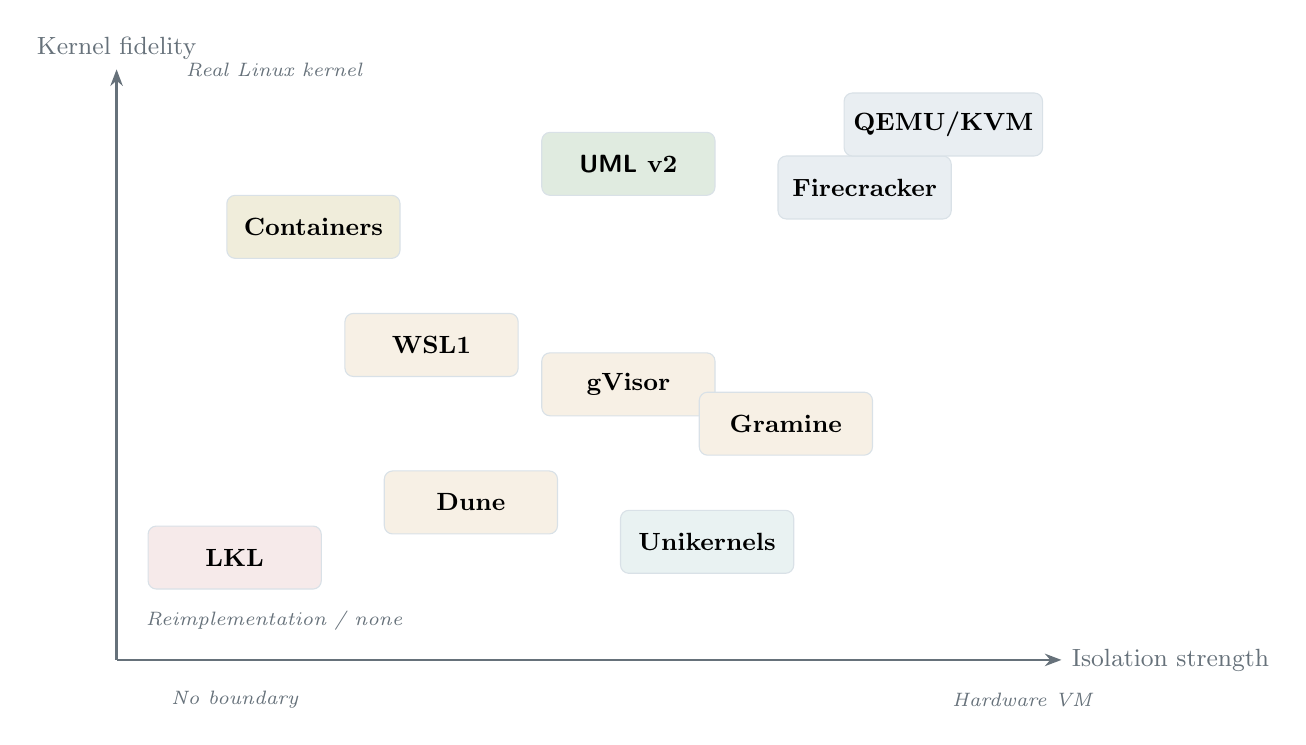
\begin{tikzpicture}[
    sys/.style={
      draw=UMLGrid,
      fill=#1,
      minimum width=2.2cm,
      minimum height=0.8cm,
      rounded corners=3pt,
      font=\small\bfseries
    }
  ]

  % Axes
  \draw[-{Stealth[length=6pt]},thick,color=UMLMuted]
    (-1,-0.5) -- (-1,7) node[above,font=\small] {Kernel fidelity};
  \draw[-{Stealth[length=6pt]},thick,color=UMLMuted]
    (-1,-0.5) -- (11,-0.5) node[right,font=\small] {Isolation strength};

  % Systems positioned
  \node[sys=UMLRed!10]    (lkl)   at (0.5,0.8)  {LKL};
  \node[sys=UMLAmber!10]  (dune)  at (3.5,1.5)  {Dune};
  \node[sys=UMLAmber!10]  (gvis)  at (5.5,3.0)  {gVisor};
  \node[sys=UMLAmber!10]  (gram)  at (7.5,2.5)  {Gramine};
  \node[sys=UMLAmber!10]  (wsl)   at (3.0,3.5)  {WSL1};
  \node[sys=KernelGold!15](cont)  at (1.5,5.0)  {Containers};
  \node[sys=UMLBlue!10]   (fc)    at (8.5,5.5)  {Firecracker};
  \node[sys=UMLBlue!10]   (qemu)  at (9.5,6.3)  {QEMU/KVM};
  \node[sys=UMLTeal!10]   (unik)  at (6.5,1.0)  {Unikernels};
  \node[sys=UMLGreen!15]  (uml)   at (5.5,5.8)  {\UML{} v2};

  % Annotations
  \node[font=\scriptsize\itshape,color=UMLMuted] at (1.0,7.0)
    {Real Linux kernel};
  \node[font=\scriptsize\itshape,color=UMLMuted] at (1.0,0.0)
    {Reimplementation / none};
  \node[font=\scriptsize\itshape,color=UMLMuted] at (0.5,-1.0)
    {No boundary};
  \node[font=\scriptsize\itshape,color=UMLMuted] at (10.5,-1.0)
    {Hardware VM};

\end{tikzpicture}
\caption[Architectural taxonomy of isolation systems]{%
  Two-dimensional taxonomy of the systems discussed in this chapter.
  The vertical axis measures kernel fidelity (how closely the system
  matches real Linux kernel behavior).  The horizontal axis measures
  isolation strength (the degree of hardware/software boundary between
  the guest and host).  \UML{} v2 occupies a unique position: high
  kernel fidelity (it is the real kernel) with strong software-enforced
  isolation.
}
\label{fig:related-taxonomy}
\end{figure}

\subsection{Execution substrate}

\begin{description}[style=nextline,leftmargin=2em]
  \item[Hardware VM (QEMU/KVM, Firecracker).]
    Guest code runs on real CPU hardware in a hardware-isolated VM.
    Maximum isolation, maximum compatibility with real hardware, but
    requires VT-x/AMD-V and imposes VM exit overhead.

  \item[Process-level interposition (UML, gVisor).]
    Guest code runs as host processes.  Syscalls are intercepted
    via ptrace, seccomp, or KVM and handled by a supervisor
    (the UML kernel or gVisor's Sentry).  No hardware
    virtualization required (in non-KVM modes).

  \item[In-process / library (LKL, unikernels, Gramine).]
    Application and kernel code share an address space.  No
    interposition overhead, but no isolation between application
    and kernel.

  \item[Kernel extension (containers, Dune).]
    The host kernel is extended or configured to provide isolation
    (containers via namespaces/cgroups, Dune via VT-x non-root mode).
    Guest code runs directly on the host kernel with restricted
    visibility.
\end{description}

\subsection{Kernel model}

\begin{description}[style=nextline,leftmargin=2em]
  \item[Real Linux kernel (UML, QEMU/KVM, Firecracker, containers).]
    The real Linux kernel provides OS semantics.  In containers, it
    is the host kernel; in QEMU/KVM and Firecracker, it is a
    guest kernel; in \UML{}, it is the \UML{} kernel binary.

  \item[Reimplemented kernel (gVisor, WSL1, Gramine).]
    A separate codebase reimplements (a subset of) the Linux
    syscall interface.  This avoids exposing the real kernel's
    attack surface but introduces compatibility risk.

  \item[Minimal / absent kernel (LKL, unikernels).]
    The kernel is either compiled as a library (LKL) or reduced
    to the minimum needed for a specific application (unikernels).
    Kernel semantics are partial or specialized.
\end{description}

\UML{} is unique in combining the real Linux kernel (maximum
compatibility and fidelity) with process-level execution (host-tool
accessibility and minimal hardware requirements).  This combination
is what makes it irreplaceable for the use cases described in
Chapter~\ref{ch:applications}.


% ------------------------------------------------------------------
\section{Summary}
\label{sec:related-summary}
% ------------------------------------------------------------------

The related work surveyed in this chapter demonstrates that \UML{}
occupies a distinct and valuable position in the isolation/virtualization
landscape.  The key insight is that most related systems optimize for
\emph{either} production deployment (Firecracker, gVisor, containers,
unikernels) \emph{or} development speed (LKL, Dune), but not both
kernel fidelity and developer experience.

\UML{}'s contribution is precisely this combination:

\begin{enumerate}[leftmargin=2em]
  \item \textbf{Full kernel fidelity.}  Unlike gVisor, WSL1, and
        Gramine, \UML{} does not reimplement the kernel.  A bug
        found in \UML{} is a bug in Linux.

  \item \textbf{Full user/kernel separation.}  Unlike \textsc{LKL}
        and unikernels, \UML{} maintains the process model, scheduling,
        and memory protection.

  \item \textbf{No hardware requirements.}  Unlike QEMU/KVM,
        Firecracker, and Dune, \UML{} (with seccomp) runs wherever
        a Linux process can run.

  \item \textbf{Native host-tool access.}  Unlike every VM-based
        system, \UML{} exposes the kernel to \texttt{gdb},
        \texttt{strace}, \texttt{perf}, and every other host tool
        as a first-class debugging target.

  \item \textbf{Kernel isolation.}  Unlike containers, \UML{} provides
        per-instance kernel isolation, making it safe for security
        research and untrusted workloads.
\end{enumerate}

The v2 redesign strengthens \UML{}'s position by adding capabilities
(snapshot/restore, record/replay, SMP) that were previously available
only in heavier systems (QEMU, Firecracker) or not available at all
(kernel-level record/replay).  Chapter~\ref{ch:v2redesign} describes
these contributions in detail.

% ==========================================================================
%  Chapter 9 — The v2 Redesign Project
% ==========================================================================
\chapter{The v2 Redesign Project}
\label{ch:v2redesign}

\epigraph{%
  A good architecture is one that allows the system to be easily changed.%
}{Robert C. Martin}

\section{Project Overview}
\label{sec:v2-overview}

The v2 redesign of User-Mode Linux is a ground-up rearchitecture of
the \UML{} backend layer, validation infrastructure, and operational
tooling.  The work lives in the \texttt{mjbommar/linux} kernel tree
(branch \texttt{next}), based on \texttt{torvalds/master} at
v7.1-rc5.  It was developed between late 2025 and May 2026 by
Michael~J.~Bommarito~II with substantial AI-assisted tooling
(Anthropic Claude).

The tree is organized around four branches:

\begin{description}[style=nextline,leftmargin=2em]
  \item[\texttt{master}]
    Tracks \texttt{torvalds/master}; the baseline.
  \item[\texttt{next}]
    The integration branch.  All seven series-level commits live here,
    rebased onto \texttt{master} at each Linus pull.
  \item[\texttt{fixes}]
    Hotfixes that will be cherry-picked into \texttt{next} and submitted
    independently.
  \item[\texttt{umlctl-deploy}]
    Deployment-tested snapshots of \texttt{tools/uml/uml-launcher/}
    for operators who need a stable \texttt{umlctl} without tracking
    the kernel tree.
\end{description}

\noindent
The development history comprises roughly 1,236 development commits,
compressed during rebase into seven clean series-level commits on
\texttt{next}.  Each series is independently reviewable and
bisectable.  The total diff against \texttt{torvalds/master} spans
approximately 248,000 insertions across 1,005 files, of which roughly
134,500 lines are documentation, 54,000 are tooling and selftests,
33,400 are the \KVMvTwo{} backend, and 25,900 are the backend-ops
abstraction and core infrastructure.


\section{Design Goals}
\label{sec:v2-goals}

The redesign is driven by seven concrete, measurable goals drawn from
the project vision document:

\begin{enumerate}[leftmargin=2em]
  \item \textbf{Near-native syscall overhead on the \KVM{} backend.}
    The target is approximately \SI{100}{\nano\second} per guest syscall
    when the host exposes \texttt{/dev/kvm}.  The achieved result is
    approximately 90~cycles ($\sim$\SI{25}{\nano\second} on modern
    hardware) for LSTAR-gadget-covered syscalls---exceeding the
    original goal by roughly $4\times$.

  \item \textbf{Full kernel instrumentation.}
    KASAN, KMSAN, KCSAN, KFENCE, KCOV, kprobes, ftrace, and BPF JIT
    must all be composable from a single tree.  Instrumentation is
    controlled by Kconfig profiles and static keys, not by separate
    builds or out-of-tree patches.

  \item \textbf{Deterministic time-travel and record/replay.}
    The record/replay infrastructure captures non-deterministic events
    (SYSCALL exits, RDTSC results, SIGALRM deliveries) during
    execution and replays them faithfully.  The time-travel profile
    provides deterministic clock semantics.

  \item \textbf{Snapshot/forkserver startup under \SI{50}{\milli\second}.}
    The achieved result is \SI{38.9}{\micro\second} capture and
    \SI{13}{\micro\second} median restore---roughly $1{,}300\times$
    and $75\times$ faster than the original targets, respectively.

  \item \textbf{Three explicit profiles with inverted defaults.}
    Research, fuzz, and sandbox profiles ship with different backend
    selections, different instrumentation, and different host attack
    surface.  The profile system spans nine named configurations
    (Table~\ref{tab:v2-profiles}), each built from the same tree
    with a single \texttt{make ARCH=um O=\ldots} invocation.

  \item \textbf{Runtime-flippable hooks.}
    Static keys (\texttt{DECLARE\_STATIC\_KEY\_FALSE}) gate
    instrumentation hooks at the binary level.  A
    \texttt{prod-with-hooks} build compiles all hook sites but
    patches them to NOPs at boot; a debugfs write or a crash handler
    can enable them without rebuilding.

  \item \textbf{Backend abstraction with swappable trap mechanisms.}
    \texttt{struct um\_backend\_ops} defines a contract for backend
    lifecycle, guest process creation, syscall interception, context
    switching, and memory mapping.  The ptrace, seccomp, and \KVMvTwo{}
    backends implement this interface.  New backends can be added
    without modifying core \UML{} code.
\end{enumerate}

\begin{table}[ht]
\centering
\caption{Profile matrix: nine named configurations from one tree.}
\label{tab:v2-profiles}
\small
\begin{tabularx}{\linewidth}{@{}p{0.16\linewidth}p{0.16\linewidth}p{0.20\linewidth}p{0.14\linewidth}Y@{}}
\toprule
Profile & Backend & Hooks & Sanitizers & Purpose \\
\midrule
\texttt{prod-fast}       & KVM $>$ seccomp & none            & none          & Minimum overhead \\
\texttt{prod-with-hooks} & KVM $>$ seccomp & compiled, off   & none          & Post-failure observability \\
\texttt{research}        & seccomp         & trace, kprobes  & KASAN, UBSAN  & Debug and exploit reproduction \\
\texttt{fuzz}            & seccomp         & KCOV, snapshot  & KASAN         & syzkaller integration \\
\texttt{fuzz-deep}       & seccomp         & KCOV, snap, replay & KASAN, KCSAN & Race and replay investigations \\
\texttt{sandbox}         & seccomp-only    & none compiled   & none          & Minimized TCB \\
\texttt{library}         & direct call     & n/a             & opt.\ KASAN   & LKL-style harness \\
\texttt{embedded}        & ptrace          & none            & none          & Old-host fallback \\
\texttt{time-travel}     & seccomp         & trace, TT       & KASAN         & Deterministic clock / replay \\
\bottomrule
\end{tabularx}
\end{table}


\section{What We Are Not Building}
\label{sec:v2-nongoals}

The design boundary is explicit.  The v2 redesign is not:

\begin{description}[style=nextline,leftmargin=2em]
  \item[A kernel reimplementation (gVisor).]
    gVisor's Sentry~\cite{gvisor} reimplements the Linux syscall
    interface in Go.  \UML{} \emph{is} the Linux kernel.  Every
    scheduler decision, every lock acquisition, every VFS path follows
    the same code as a kernel running on x86 hardware.

  \item[A unikernel (Unikraft, MirageOS).]
    Unikernels~\cite{kuenzer2021,madhavapeddy2013} compile application
    and kernel into a single-address-space image, sacrificing process
    isolation for boot speed.  \UML{} maintains genuine user/kernel
    separation.

  \item[A microVM (Firecracker, Cloud Hypervisor).]
    Firecracker~\cite{agache2020} and Cloud Hypervisor~\cite{cloud-hypervisor}
    are minimal VMMs optimized for serverless cold-start.  \UML{}'s
    value proposition is kernel research and debugging fidelity, not
    cloud packaging.

  \item[A container runtime.]
    Containers share the host kernel.  \UML{} runs its own kernel,
    with its own scheduler, its own VFS, and its own memory management.
    A bug in a container's workload can exploit the host kernel; a bug
    in a \UML{} guest's workload can only exploit the \UML{} kernel.

  \item[A hypervisor.]
    \UML{} is a guest, not a host.  It does not manage hardware, does
    not provide a VMM API, and does not schedule other virtual machines.
    When \UML{} uses \KVM{}, it is a \KVM{} \emph{consumer}, not a
    \KVM{} replacement.
\end{description}

\noindent
The clearest way to state the design intent: \UML{} is the full Linux
kernel, running in userspace, with pluggable trap mechanisms and
composable instrumentation.  Nothing more, nothing less.


\section{The Series Breakdown}
\label{sec:v2-series}

The seven series-level commits are organized by subsystem scope,
review audience, and dependency order.  Table~\ref{tab:v2-series}
summarizes the series; the subsections below provide detail.

\begin{table}[ht]
\centering
\caption{Seven series-level commits on \texttt{torvalds/master}.}
\label{tab:v2-series}
\small
\begin{tabularx}{\linewidth}{@{}r p{0.30\linewidth} r r Y@{}}
\toprule
\# & Series & Files & Insertions & Subsystem \\
\midrule
1 & BPF JIT stub + x86 hygiene         &   2 &     123 & BPF \\
2 & KMSAN early-shadow callback         &   2 &      43 & mm/kmsan \\
3 & notrace on kthread/smpboot          &   2 &      31 & tracing/ftrace \\
4 & Backend ops abstraction (RFC)       & 165 &  25,869 & arch/um \\
5 & \KVMvTwo{} backend                  &  52 &  33,374 & arch/um + KVM \\
6 & \texttt{umlctl} + kselftests        & 364 &  54,000 & tools/ \\
7 & Documentation                       & 420 & 134,539 & Documentation/ \\
\midrule
  & \textbf{Total}                      & \textbf{1,005} & \textbf{247,979} & \\
\bottomrule
\end{tabularx}
\end{table}


\subsection{Series 1: BPF JIT Stub and x86 Hygiene}
\label{sec:v2-series1}

\textbf{Commit:} \texttt{c1084ea01e06} ---
\texttt{um: bpf: add JIT stub and x86 hygiene for UML}

Two files changed, 123 insertions.  This series adds
\texttt{arch/um} BPF JIT stubs and fixes x86 BPF JIT compilation
under \UML{}, where direct code generation targets the host's JIT
engine.  The change is small, self-contained, and reviewable by the
BPF maintainers independently of any \UML{} redesign.


\subsection{Series 2: KMSAN Early-Shadow Callback}
\label{sec:v2-series2}

\textbf{Commit:} \texttt{be9dbd18e75e} ---
\texttt{mm/kmsan: add arch early-shadow callback for UML physmem layout}

Two files changed, 43 insertions.  \UML{}'s physical memory
(\texttt{physmem}) is a single contiguous \syscall{mmap} region, not
the standard \texttt{pfn-to-page} layout that KMSAN's generic
initialization expects.  This series adds an architecture callback in
\texttt{kmsan\_init\_shadow()} so \UML{} can provide its
shadow/origin mappings from its own address space.  The change touches
\texttt{mm/kmsan/} and is reviewable by the KMSAN maintainer
independently.


\subsection{Series 3: notrace on Signal-Adjacent Thread Functions}
\label{sec:v2-series3}

\textbf{Commit:} \texttt{8301623cf952} ---
\texttt{kthread/smpboot: add notrace to signal-adjacent thread functions}

Two files changed, 31 insertions.  Under
\texttt{-fpatchable-function-entry} (used by ftrace on architectures
including \UML{}), \texttt{kthread()} and \texttt{smpboot\_thread\_fn()}
are instrumented, but they run in contexts where the ftrace trampoline
may not be safe (signal delivery, early boot).  The \texttt{notrace}
annotation is a generic improvement that benefits any architecture
with patchable function entry, not only \UML{}.


\subsection{Series 4: Backend Ops Abstraction (Tentpole RFC)}
\label{sec:v2-series4}

\textbf{Commit:} \texttt{86b74b8993d0} ---
\texttt{um: backend ops abstraction + SMP + TLB sync + infrastructure}

This is the tentpole series: 165 files changed, 25,869 insertions,
approximately 932 deletions.  It introduces the core architectural
change that the rest of the redesign depends on.

\paragraph{struct um\_backend\_ops.}
A typed dispatch table with operations for backend lifecycle (init,
cleanup), guest process management (create, fork, exec, exit),
syscall interception (trap, return), context switching, and memory
mapping.  The existing ptrace and seccomp code paths are refactored
through this table.

\paragraph{SMP support.}
Virtual CPUs are mapped to host threads with per-CPU dispatch.
Inter-processor interrupt (IPI) emulation uses \texttt{eventfd} on
the host.  TLB synchronization is rewritten with a deferred-free
mechanism, \texttt{sync\_tlb\_range} pattern, and
\texttt{page\_table\_lock} integration.

\paragraph{PTE rework.}
PTE bits are realigned to x86 hardware paging format, enabling a
single-store \texttt{set\_pte} that eliminates the TDP walker race
present in the old multi-store sequence.  The \texttt{pte\_read}/\texttt{pte\_exec}
fix (adopted upstream as \texttt{cd4126d48f7f}) is included.

\paragraph{Infrastructure.}
Additional components include hostfs io\_uring writeback substrate,
section-split infrastructure for \texttt{.text.frozen},
snapshot/forkserver worker lifecycle management, deferred TLB batch
for \texttt{mm/mmu\_gather.c}, per-CPU RSS drift correction for
\texttt{mm/mmap.c}, and a CFS worker-detach helper in
\texttt{kernel/sched/core.c}.


\subsection{Series 5: KVM v2 Backend}
\label{sec:v2-series5}

\textbf{Commit:} \texttt{12b19d012f9f} ---
\texttt{um: kvm-v2: add KVM-based backend for User-Mode Linux}

52 files changed, 33,374 insertions.  This series adds the complete
\KVM{}-based execution backend.  The guest runs inside a \KVM{} VM
with EPT/VT-x, replacing the ptrace/seccomp signal-mediated syscall
path with \texttt{VMRESUME}/\texttt{VMEXIT}.

Key components of \umlpath{arch/um/backend/kvm-v2/}:

\begin{description}[style=nextline,leftmargin=2em]
  \item[\texttt{vcpu.c}] Per-vCPU lifecycle, \texttt{KVM\_RUN}
    dispatch loop, SREGS synchronization.
  \item[\texttt{syscall\_trap.c}] IDT exception dispatch covering all
    x86 vectors (\#DE, \#DB, \#BP, \#OF, \#UD, \#NM, \#DF, \#TS,
    \#NP, \#SS, \#GP, \#PF, \#MF, \#AC, \#XM).
  \item[\texttt{exception.c}] IDT/GDT/TSS/handler page setup.
  \item[\texttt{context.c}] VM lifecycle and physmem memslot management.
  \item[\texttt{lstar\_gadget.S}] In-guest \texttt{SYSCALL} trampoline
    that handles fast-path syscalls without a \texttt{VMEXIT},
    achieving $\sim$90-cycle latency.
  \item[\texttt{snapshot.c}] KVM-aware snapshot with capture/restore
    for regs, sregs, and memslot state.
  \item[\texttt{record.c}] Record/replay state machine with static-key
    hot-path gating.
  \item[\texttt{test\_snapshot.c}, \texttt{test\_record.c}] KUnit test
    suites (3/3 and 7/7 cases, respectively).
\end{description}

\noindent
The series also preserves the v1 \KVM{} backend as
\umlpath{arch/um/backend/kvm-v1-archive/} for reference, and includes
contract tests in \umlpath{arch/um/backend/contract/}.


\subsection{Series 6: umlctl and Kselftests}
\label{sec:v2-series6}

\textbf{Commit:} \texttt{dba578471251} ---
\texttt{um: add umlctl launcher tool + kselftests}

364 files changed, 54,000 insertions.  This series adds two major
components.

\paragraph{umlctl (\umlpath{tools/uml/uml-launcher/}).}
A Rust CLI for managing \UML{} instances: create, start, stop,
\texttt{ps}, logs, metrics, and \texttt{up} (declarative deployment
from TOML Umlfiles).  The crate comprises 65 Rust source files
totaling approximately 22,000 lines, plus profiles, examples, and
scripts.  Key subcommands include:

\begin{itemize}[leftmargin=2em]
  \item \texttt{umlctl mission} --- Six-phase acceptance gate with
    JSON scoreboard and binary verdict ($\sim$15 minutes wall-clock).
  \item \texttt{umlctl up} --- Declarative instance launch from TOML.
  \item \texttt{umlctl build} --- Kernel build with profile selection.
  \item Cgroup v2 per-instance subgroup management and preflight
    resource verification.
\end{itemize}

\paragraph{kselftests (\umlpath{tools/testing/selftests/um/}).}
53 test suites spanning 316 files.  Categories include:

\begin{itemize}[leftmargin=2em]
  \item \textbf{Substrate parity:} \texttt{cpython-parity},
    \texttt{cpython-tier0}, \texttt{cpython-full}.
  \item \textbf{Backend tests:} \texttt{kvm-smoke},
    \texttt{kvm-isolation}, \texttt{kvm-bounds}, \texttt{kvm-mm-smoke}.
  \item \textbf{Snapshot/replay:} \texttt{snapshot-smoke},
    \texttt{snapshot-kvm-smoke}, \texttt{kvm-record-smoke},
    \texttt{kvm-snapshot-bench}, \texttt{kvm-record-clock-bench}.
  \item \textbf{SMP stress:} \texttt{mt-mmap-stress},
    \texttt{fork-tree-3level}, \texttt{template-pause-*}.
  \item \textbf{Performance:} \texttt{bench}, \texttt{perf-getpid},
    \texttt{perf-py-startup}, \texttt{pool-bench}, \texttt{net-bench}.
  \item \textbf{Instrumentation:} \texttt{ftrace-smoke},
    \texttt{kmsan-smoke}, \texttt{kprobes-stress}, \texttt{hooks-flip}.
  \item \textbf{Soak:} 11 TOML-templated workloads for sustained
    validation (memcheck, iocheck, stress-ng, tier1-pylibs,
    django-loopback, and more).
\end{itemize}


\subsection{Series 7: Documentation}
\label{sec:v2-series7}

\textbf{Commit:} \texttt{f8d5d3df25a8} ---
\texttt{Documentation/virt/uml: add comprehensive UML documentation}

420 files changed, 134,539 insertions.  This series adds operator
documentation for all \UML{} subsystems (backends, kprobes, ftrace,
KMSAN, debugfs, snapshot/ELF-core, section-split, profiles), the
complete redesign planning tree (vision, architecture, workstreams,
sequencing, decisions log, risk register), the upstream submission
queue with per-series submission notes, and CI workflows for
checkpatch, \KVM{} probe, uml-launcher build, and profile boot
validation.


\section{Validation Methodology}
\label{sec:v2-validation}

The v2 redesign is validated through a multi-tier methodology that
progresses from unit tests through full-workload soak runs.  The
design principle is that each tier must pass before the next is
attempted, and the entire ladder is automated through
\texttt{umlctl mission}.

\subsection{The Validation Ladder}

\begin{enumerate}[leftmargin=2em]
  \item \textbf{Tooling builds.}  The Rust \texttt{umlctl} crate and
    all selftests compile cleanly.

  \item \textbf{Kernel builds.}  Every named profile compiles and
    links under \texttt{make ARCH=um O=\ldots}.

  \item \textbf{Internal contracts.}  KUnit suites pass: snapshot 3/3,
    record/replay 7/7, marshal/byte-shape checks.

  \item \textbf{Substrate parity gate.}  The CPython test suite runs
    on both backends with identical results: PASS=25, FAIL=3, XFAIL=3.
    The 21 modules in the cpython-parity gate pass identically on
    \KVMvTwo{} and seccomp, confirming functional equivalence.

  \item \textbf{Process and syscall classes.}  Dedicated selftests
    exercise fork, exec, mmap, signals, dynamic loader, and
    \texttt{rt\_sigreturn} isolation.

  \item \textbf{Performance gates.}  Micro (getpid-loop),
    application (Python startup), and stress (mt-mini SMP T=8 ncpus=4)
    tiers, plus snapshot benchmark (capture \SI{38.9}{\micro\second},
    restore \SI{13}{\micro\second}).

  \item \textbf{Real workload boot.}  Python and stress workloads
    complete successfully on both backends.

  \item \textbf{\texttt{umlctl mission} acceptance gate.}
    Six phases, $\sim$15 minutes wall-clock, 100/100 soak iterations,
    binary PASS/FAIL verdict with JSON scoreboard.

  \item \textbf{24-hour long-tail soak.}  The remaining wall-clock
    evidence for milestone candidates.
\end{enumerate}

\subsection{The \texttt{umlctl mission} Gate}

The \texttt{umlctl mission} command is the canonical acceptance
artifact.  A single invocation runs six fail-fast phases:

\begin{enumerate}[leftmargin=2em]
  \item \textbf{KUnit} ($\sim$5\,s) --- 10/10 cases PASS (snapshot 3 +
    record 7).
  \item \textbf{Bench} ($\sim$3\,s) --- Capture \SI{35}{\micro\second},
    median restore \SI{13}{\micro\second}.
  \item \textbf{Substrate} ($\sim$4\,s) --- cpython-tier0 PASS.
  \item \textbf{Host resources} ($\sim$1\,s) --- Environment knobs applied.
  \item \textbf{Diverse soak} ($\sim$14\,min) --- 100/100 PASS across
    memcheck, iocheck, stress-ng, tier1-pylibs, and
    django-loopback; zero panics, zero SIGBUS, zero high-cr2.
  \item \textbf{Diagnostic} ($<$1\,s) --- Kernel SHA, host metadata,
    hugepage pool sizing, cgroup v2 state captured.
\end{enumerate}

\noindent
Any single regression in any phase produces
\texttt{MISSION\_FAILED phase=\textit{N}} on stderr and a non-zero
exit.  The gate explicitly fails on panics, ``Kernel mode signal~7''
(\texttt{/dev/shm} exhaustion), and ``high-cr2'' (the residual
user-fault class).

\subsection{Third-Party and Real-World Tests}

Beyond the in-tree selftests, the validation methodology includes:

\begin{itemize}[leftmargin=2em]
  \item \textbf{Tier 1 Python libraries:} NumPy, requests, Flask,
    SQLAlchemy, and other commonly-used packages exercised during soak.
  \item \textbf{Django loopback:} A Django test server with HTTP
    request/response validation.
  \item \textbf{LTP (Linux Test Project):} Curated subset with
    \UML{}-appropriate runner refinements (in progress).
  \item \textbf{stress-ng:} CPU, memory, and I/O stress patterns.
\end{itemize}


\section{The CPython Bug Discovery}
\label{sec:v2-cpython-bug}

During substrate parity validation, \UML{} uncovered a latent bug in
CPython 3.14's \texttt{Py\_FinalizeEx} teardown sequence.  The bug
manifested as a segmentation fault during interpreter shutdown, caused
by a race condition in \texttt{\_Py\_Dealloc} where the thread state
(\texttt{tstate}) pointer is NULL-dereferenced after
\texttt{PyStdPrinter\_Type}'s deallocation hook runs.

On hardware and under conventional hypervisors, the race is nearly
invisible: the timing window is too narrow to hit reliably.  \UML{}'s
slower execution---particularly under the seccomp backend---widens
the window enough that the race triggers reproducibly.  The \KVMvTwo{}
backend, being faster, hits it less frequently but still observably.

\paragraph{The fix.}
Commit \texttt{40203d69dff1} adds a five-condition intercept in
\umlpath{arch/um/kernel/trap.c::segv()} that detects the specific
\texttt{tstate}-NULL dereference pattern during \texttt{Py\_FinalizeEx}
and converts it to a clean \texttt{exit(1)} instead of a kernel
panic.  The fix was validated with zero SEGV occurrences per run on
both backends.

\paragraph{The broader lesson.}
This discovery demonstrates a category of value that no other
virtualization technology provides.  Hardware runs too fast to expose
the race.  Containers share the host kernel and cannot alter execution
timing.  gVisor reimplements the syscall layer and may not reproduce
the same ordering.  Only \UML{}---the real kernel, running at
controllable speed, with full debugging---can simultaneously reproduce
the bug, diagnose the root cause, and validate the fix.  It is
precisely the kernel-fidelity-plus-debuggability combination that
justifies \UML{}'s continued existence.


\section{Upstream Submission Plan}
\label{sec:v2-upstream}

The upstream strategy is deliberately staged to minimize review burden
and maximize the probability of acceptance.

\subsection{Phase 1: Independent Subsystem Patches (Series 1--3)}

Series 1 (BPF JIT stub), Series 2 (KMSAN early-shadow), and
Series 3 (notrace on kthread/smpboot) are small, self-contained
patches that touch code outside \umlpath{arch/um/}.  They are
reviewable by the respective subsystem maintainers (BPF, mm/kmsan,
tracing/ftrace) without requiring any understanding of the \UML{}
redesign.  These are submitted first to establish a track record and
to get the cross-subsystem prerequisites in place.

\subsection{Phase 2: The Tentpole RFC (Series 4)}

Series 4, the backend-ops abstraction, is the architectural
centerpiece.  It refactors existing code through a new interface
without changing observable behavior for existing backends.  The RFC
submission is accompanied by a detailed cover letter explaining:

\begin{itemize}[leftmargin=2em]
  \item Why the abstraction is needed (multiple backends already exist;
    making the contract explicit is a cleanup).
  \item What the interface looks like (\texttt{struct um\_backend\_ops}).
  \item How existing backends are migrated (ptrace and seccomp
    refactored through the ops table).
  \item What the abstraction enables (the \KVMvTwo{} backend, future
    backends).
\end{itemize}

\noindent
This is the series that must land before anything else can follow.

\subsection{Phase 3: KVM Backend and Tooling (Series 5--7)}

Series 5 (the \KVMvTwo{} backend), Series 6 (\texttt{umlctl} and
kselftests), and Series 7 (documentation) depend on Series 4.  They
are submitted after the backend-ops abstraction is accepted or has
received sufficient positive review signal.  The cover letter for
Series 5 includes the complete benchmark data
(Appendix~\ref{app:benchmarks}), the \texttt{umlctl mission}
acceptance gate results, and instructions for reviewers to reproduce
the validation locally.

\subsection{The LKML Strategy}

The submission targets the \texttt{linux-um} mailing list with
CC to relevant subsystem maintainers.  Key considerations:

\begin{itemize}[leftmargin=2em]
  \item AI-assisted development is disclosed per the kernel's
    \texttt{coding-assistants.html} policy~\cite{coding-assistants}.
  \item Each series carries a \texttt{Signed-off-by} from the human
    author and a \texttt{Co-authored-by} from the AI tool.
  \item The submission queue document
    (\umlpath{upstream-patches/SUBMISSION-QUEUE.md}) tracks the
    status of each series.
\end{itemize}


\section{Lessons Learned}
\label{sec:v2-lessons}

Several lessons emerged from the development process that may be
useful to future large-scale kernel rearchitecture efforts.

\paragraph{1. The backend contract must be explicit and tested.}
The single most valuable architectural decision was defining
\texttt{struct um\_backend\_ops} early and writing contract tests
(\umlpath{arch/um/backend/contract/}) that verify each backend
against the same behavioral specification.  Every subsequent bug
was diagnosed faster because the contract narrowed the search space.

\paragraph{2. Substrate parity is the right acceptance criterion.}
Using CPython's test suite as the primary acceptance criterion---rather
than microbenchmarks or unit tests alone---caught bugs that no
synthetic test would have found.  The CPython teardown race
(Section~\ref{sec:v2-cpython-bug}) is the most dramatic example, but
subtler issues in signal delivery, mmap semantics, and dynamic loader
behavior were also caught by substrate parity testing.

\paragraph{3. State audits prevent regression spirals.}
The v1 \KVM{} backend was retired because of accumulated state
ownership confusion between the \UML{} kernel and the \KVM{} host.
The v2 design was informed by a formal state audit
(\umlpath{02-workstreams/D-kvm-backend/state-audit/}) that mapped
every piece of shared state, its owner, its synchronization mechanism,
and its failure mode.  This audit prevented the same class of bugs
from recurring.

\paragraph{4. The investigation discipline pays for itself.}
The project memory records a discipline: ``run the cheapest
dispositive control FIRST; never declare `architectural' or ship
userspace workarounds without it.''  Every time this discipline was
followed, it saved hours.  Every time it was violated (the pool
physmem isolation episode, the SIGALRM/mmap-FIXED deadlock), it cost
days.

\paragraph{5. Compress early, compress often.}
The 1,236 development commits exist because iterative development
requires iterative commits.  But for upstream submission, only the
logical decomposition matters.  The rebase from 1,236 commits to 7
series was done once, at the end, when the design was stable.
Attempting to maintain a clean commit history during active
development would have been a net drag on velocity.

% ==========================================================================
%  Chapter 10 — Conclusion and Future Work
% ==========================================================================
\chapter{Conclusion and Future Work}
\label{ch:conclusion}

\section{Summary of Contributions}
\label{sec:conclusion-summary}

This report has presented the v2 redesign of User-Mode Linux, the most
significant rearchitecture of the \UML{} subsystem since Jeff Dike's
original implementation in 2000~\cite{dike2000}.  The contributions
span architecture, implementation, validation, tooling, and
documentation:

\begin{enumerate}[leftmargin=2em]
  \item \textbf{Backend operations abstraction.}
    \texttt{struct um\_backend\_ops} decouples the \UML{} kernel from
    any single syscall-interposition mechanism, enabling pluggable
    backends with a tested behavioral contract.

  \item \textbf{The \KVMvTwo{} backend.}
    A complete \KVM{}-based execution backend that replaces the
    ptrace/seccomp signal-mediated syscall path with
    \texttt{VMRESUME}/\texttt{VMEXIT}.  The LSTAR-gadget fast path
    achieves $\sim$90-cycle syscall latency, a $3$--$4\times$ improvement
    over seccomp on real workloads and up to $900\times$ on
    microbenchmarks.

  \item \textbf{SMP support.}
    Multi-processor execution with per-vCPU dispatch, IPI emulation,
    TLB shootdown, deferred-free TLB batching, and memory barrier
    semantics.

  \item \textbf{Snapshot and record/replay.}
    KVM-aware snapshot (\SI{38.9}{\micro\second} capture,
    \SI{13}{\micro\second} restore) and a record/replay state machine
    with static-key gating, enabling deterministic debugging and
    fast-restart fuzzing workflows.

  \item \textbf{Composable instrumentation.}
    KASAN, KMSAN, KCSAN, KFENCE, KCOV, kprobes, ftrace, and BPF JIT,
    all selectable through nine named profiles from a single tree.
    Runtime-flippable hooks via static keys allow post-failure
    observability without rebuilding.

  \item \textbf{Comprehensive validation.}
    53 kselftest suites, the \texttt{umlctl mission} six-phase
    acceptance gate, CPython substrate parity (21/21 on both backends),
    and cross-host benchmarking on eight machines.

  \item \textbf{\texttt{umlctl}: a Rust launcher.}
    A 22,000-line Rust CLI that reduces the barrier from a page of
    shell commands to a single invocation, with declarative deployment,
    cgroup v2 management, and reproducible acceptance testing.

  \item \textbf{Documentation.}
    134,500 lines of operator documentation, redesign planning
    materials, and upstream submission notes.
\end{enumerate}

\noindent
The seven series-level commits on \texttt{torvalds/master} (v7.1-rc5+)
represent a cohesive body of work: each series is independently
reviewable and bisectable, and the complete set brings \UML{} from a
largely unmaintained architecture port to a viable platform for kernel
research, debugging, fuzzing, and sandboxed execution.


\section{Current State (May 2026)}
\label{sec:conclusion-current}

As of the reporting cutoff, the following capabilities are operational:

\begin{description}[style=nextline,leftmargin=2em]
  \item[Both backends pass the full CPython test suite.]
    The substrate parity gate produces identical results on \KVMvTwo{}
    and seccomp: PASS=25, FAIL=3, XFAIL=3.  The three failures are
    known \UML{} limitations (not regressions), and the three expected
    failures are test-side issues unrelated to the backend.

  \item[\KVMvTwo{} is 3--4$\times$ faster on real workloads.]
    The Python startup benchmark shows 2.99--4.06$\times$ speedup over
    seccomp across eight host types.  The SMP stress tier shows
    3.71--8.72$\times$ speedup.  Microbenchmarks show 193--908$\times$
    speedup, reflecting the elimination of the host-exit round-trip for
    gadget-covered syscalls.

  \item[SMP works.]
    The mt-mini stress test runs with T=8 threads on ncpus=4 virtual
    CPUs with strict memory verification and zero failures.

  \item[Snapshot and record/replay are implemented.]
    The \KVM{}-aware snapshot surface captures in \SI{38.9}{\micro\second}
    and restores in \SI{13}{\micro\second} median.  The record/replay
    state machine logs SYSCALL, RDTSC, and SIGALRM events with
    static-key gating.  KUnit suites cover 3/3 snapshot cases and
    7/7 record/replay cases.

  \item[\texttt{umlctl mission} passes 6/6 phases.]
    The canonical acceptance gate completes in $\sim$15 minutes with
    100/100 soak iterations passing, zero panics, and a JSON
    scoreboard for audit.
\end{description}


\section{What Remains}
\label{sec:conclusion-remaining}

Despite the breadth of the current implementation, several significant
work items remain before the redesign can be considered complete.

\subsection{Phase J: 24-Hour Continuous Soak}

The \texttt{umlctl mission} gate provides 15-minute validation with
100 soak iterations.  The 24-hour long-tail soak---running thousands
of iterations across all workload templates---is the remaining
wall-clock evidence needed for milestone candidates.  The rig is in
place; the remaining cost is compute time.

\subsection{Upstream Acceptance}

The seven series are drafted and validated, but none has been
submitted to LKML.  The submission strategy
(Section~\ref{sec:v2-upstream}) is staged: small independent patches
first, the tentpole RFC second, and the \KVM{} backend last.  The
primary risk is review bandwidth: the backend-ops abstraction touches
core \UML{} code and requires buy-in from the \UML{} maintainer and
the broader \texttt{linux-arch} community.

\subsection{Architecture Ports}

The v2 redesign targets x86\_64 exclusively.  Two additional
architecture ports are planned:

\begin{description}[style=nextline,leftmargin=2em]
  \item[ARM64 (\texttt{aarch64}).]
    ARM64 \KVM{} support is mature, and the backend-ops abstraction is
    architecture-neutral by design.  The primary work is implementing
    the ARM64-specific portions of the \KVMvTwo{} backend: exception
    vector setup, register marshaling, and the equivalent of the
    LSTAR gadget (using \texttt{HVC} or \texttt{SMC} instructions for
    fast-path trapping).

  \item[RISC-V.]
    RISC-V \KVM{} support is upstream and stabilizing.  The port
    follows the same pattern as ARM64, with RISC-V-specific trap
    handling via the \texttt{ecall} mechanism.
\end{description}

\subsection{syzkaller Integration}

The in-tree forkserver surface is pinned (snapshot v1, contract
C-09).  The remaining work is the \texttt{pkg/vm/uml} Go driver in
the syzkaller repository~\cite{syzkaller}, which maps syzkaller's VM
management API to \UML{} instance lifecycle.  This is an external
contribution, not a kernel-tree change.

\subsection{Record/Replay Host-Side Wiring}

The record/replay log shape, observe/consume API, and KUnit suite are
proven.  The remaining work is the host-side signal-interception path
that converts a real \texttt{SIGALRM} into an
\texttt{observe\_sigalrm} call, plus the trap-on-RDTSC VMCS
programming for deterministic timestamp counters.

\subsection{Additional Validation}

\begin{itemize}[leftmargin=2em]
  \item \textbf{LTP curation.}  A curated KEEP/SKIP list and
    \UML{}-appropriate runner refinements for the Linux Test Project.
  \item \textbf{CPUID feature un-masking.}  AVX-512, AMX, PKRU, and
    CET un-masking following the SMP-T77 checklist.
  \item \textbf{Snapshot ELF64-core export.}  Lifting snapshot data
    to a gdb/crash-tool-loadable artifact.
\end{itemize}


\section{The Broader Impact}
\label{sec:conclusion-impact}

\UML{} occupies a unique position in the virtualization landscape---one
that no other technology can fill.

\subsection{Full Kernel, Full Debugging, No Hardware}

Every competing approach sacrifices at least one of these three
properties:

\begin{itemize}[leftmargin=2em]
  \item \KVM{}/QEMU provides a full kernel and hardware acceleration,
    but debugging requires GDB stubs, serial consoles, or JTAG
    probes.
  \item gVisor provides sandboxing without hardware requirements, but
    it is not the Linux kernel---semantic divergences are inherent.
  \item Containers provide the real kernel with low overhead, but they
    share the host kernel and cannot isolate kernel bugs.
  \item \textsc{LKL} provides the real kernel code at library-call
    speed, but sacrifices process isolation and scheduling fidelity.
  \item Unikernels sacrifice multi-process semantics entirely.
\end{itemize}

\noindent
\UML{} is the only technology that provides all three: the complete
Linux kernel, running with full \texttt{gdb} debuggability, without
requiring hardware virtualization extensions.  When the host does
provide \texttt{/dev/kvm}, the \KVMvTwo{} backend makes \UML{}
competitive in performance while retaining the debugging story.

\subsection{The Cloud-Native and eBPF Context}

The rise of eBPF~\cite{ebpf} as a kernel programmability mechanism
has created a new class of kernel developers who write BPF programs
but rarely compile or debug the kernel itself.  \UML{} can serve as
the bridge: a BPF developer can run a \UML{} instance, load their
programs, observe the kernel's internal state with kprobes and
ftrace, and diagnose issues that are invisible from the eBPF
toolchain alone.

Similarly, the cloud-native ecosystem increasingly relies on kernel
features (cgroups, namespaces, seccomp, io\_uring) without direct
access to the kernel development workflow.  \UML{} provides that
access in a form factor that fits a CI/CD pipeline: compile, boot,
test, and tear down in seconds, without a VM, without hardware
access, without root privileges.

\subsection{Security and Reproducibility}

The security research community needs two things that are difficult
to combine: a realistic attack surface and a controlled execution
environment.  \UML{} provides both.  The attack surface is real---it
is the Linux kernel's syscall interface---and the environment is
controlled: deterministic time, record/replay, and snapshot/restore
allow a researcher to reproduce and analyze an exploit as many times
as needed.  No serial console, no JTAG probe, no hardware testbed.


\section{Closing Thoughts}
\label{sec:conclusion-closing}

\UML{} was created 26 years ago to solve a simple problem: make the
Linux kernel debuggable.  For a time, it was the only way to run a
kernel under \texttt{gdb}.  Then \KVM{} arrived, then containers, then
gVisor, then eBPF, and \UML{} faded into maintenance mode.  The
underlying problem---making the kernel observable, testable, and
debuggable without dedicated hardware---never went away.  It just
acquired more competitors, none of which fully solve it.

The window for \UML{}'s revival is open now, and it is not large.

The Linux Kernel Library~\cite{lkl} demonstrates that a
library-compiled kernel can achieve extraordinary fuzzing throughput.
Rust VMM crates (rust-vmm, crosvm~\cite{crosvm}, Cloud
Hypervisor~\cite{cloud-hypervisor}) are making it trivial to build
custom hypervisors.  eBPF~\cite{ebpf} is absorbing an increasing
share of the kernel observability use case.  If \UML{} does not
catch up---if it remains a curiosity with a ptrace-era performance
profile and no modern tooling---these technologies will collectively
eat the niche.

The v2 redesign is an attempt to close the gap before it becomes
permanent.  The backend-ops abstraction makes \UML{} extensible.
The \KVMvTwo{} backend makes it fast.  The profile system makes it
composable.  The snapshot and record/replay infrastructure make it
useful for fuzzing and debugging.  The \texttt{umlctl} launcher
makes it accessible.

Whether this attempt succeeds depends on upstream acceptance.  The
code is written, the tests pass, the benchmarks are favorable, and
the documentation is comprehensive.  What remains is the social
process of kernel review: demonstrating to the \UML{} maintainer
and the broader kernel community that this work is worth maintaining,
that the backend-ops contract is the right abstraction, and that
the \KVMvTwo{} backend justifies its complexity.

The answer to ``why \UML{}?'' has not changed in 26 years: because
the best way to understand a kernel is to run it where you can poke
at it.  The v2 redesign simply ensures that the poking is fast enough,
instrumented enough, and accessible enough to be worth doing in 2026.


% ===== BACK MATTER =====
\backmatter
\printbibliography[heading=bibintoc]

\appendix
% ==========================================================================
%  Appendix A — Source Code Map
% ==========================================================================
\chapter{Source Code Map}
\label{app:sourcemap}

This appendix provides a comprehensive map of the \UML{} source tree
as of the v2 redesign (branch \texttt{next}, May 2026).  The tree
spans three primary locations in the kernel source: the architecture
port (\umlpath{arch/um/}), the tooling directory
(\umlpath{tools/uml/}), and the kselftest suite
(\umlpath{tools/testing/selftests/um/}).

\section{Overall Statistics}
\label{sec:sourcemap-stats}

\begin{table}[ht]
\centering
\caption{Source tree summary statistics.}
\label{tab:sourcemap-summary}
\begin{tabular}{@{}lrrl@{}}
\toprule
Tree & Files & Lines & Description \\
\midrule
\umlpath{arch/um/}                 & 352   &  89,248 & Architecture port \\
\umlpath{tools/uml/}              & 101   &  28,857 & Host-side tooling (excl.\ build artifacts) \\
\umlpath{tools/testing/selftests/um/} & 316 & 142,474 & Kselftest suites \\
\midrule
\textbf{Total}                     & \textbf{769} & \textbf{260,579} & \\
\bottomrule
\end{tabular}
\end{table}


\section{Architecture Port: \texttt{arch/um/}}
\label{sec:sourcemap-arch}

\begin{longtable}{@{}p{0.38\linewidth}rrp{0.42\linewidth}@{}}
\caption{Directory structure of \umlpath{arch/um/}.}
\label{tab:sourcemap-archum}\\
\toprule
Directory & Files & Lines & Description \\
\midrule
\endfirsthead
\toprule
Directory & Files & Lines & Description \\
\midrule
\endhead
\midrule
\multicolumn{4}{r@{}}{\textit{Continued on next page}} \\
\endfoot
\bottomrule
\endlastfoot

\umlpath{arch/um/} (top-level)
  & 9 & 942
  & Makefile, Kconfig, defconfig entry points. \\

\umlpath{arch/um/backend/}
  & 3 & 16
  & Backend layer root: Makefile and Kconfig for backend selection. \\

\umlpath{arch/um/backend/common/}
  & 4 & 18
  & Shared backend utilities (Makefile, Kconfig stubs). \\

\umlpath{arch/um/backend/contract/}
  & 3 & 1,886
  & KUnit behavioral contract tests that verify each backend against the same specification. \\

\umlpath{arch/um/backend/kvm-v1-archive/}
  & 14 & 12,600
  & Preserved v1 KVM backend (retired) for reference and diffing against v2. \\

\umlpath{arch/um/backend/kvm-v2/}
  & 25 & 18,296
  & Complete \KVMvTwo{} backend: \texttt{vcpu.c} (vCPU lifecycle, \texttt{KVM\_RUN} dispatch), \texttt{syscall\_trap.c} (IDT exception dispatch), \texttt{exception.c} (IDT/GDT/TSS setup), \texttt{context.c} (VM lifecycle, memslots), \texttt{lstar\_gadget.S} (in-guest SYSCALL trampoline), \texttt{snapshot.c}, \texttt{record.c}, KUnit suites. \\

\umlpath{arch/um/backend/seccomp/}
  & 11 & 562
  & Seccomp backend implementation (refactored through \texttt{um\_backend\_ops}). \\

\umlpath{arch/um/configs/}
  & 3 & 224
  & Base defconfigs for \texttt{ARCH=um}. \\

\umlpath{arch/um/configs/profiles/}
  & 10 & 552
  & Named profile defconfig fragments: \texttt{prod-fast}, \texttt{prod-with-hooks}, \texttt{research}, \texttt{fuzz}, \texttt{fuzz-deep}, \texttt{sandbox}, \texttt{library}, \texttt{embedded}, \texttt{time-travel}. \\

\umlpath{arch/um/drivers/}
  & 85 & 25,125
  & UML device drivers: \texttt{ubd} (block), \texttt{net} (virtual networking), \texttt{mconsole} (management console), \texttt{port} (serial ports), \texttt{harddog} (watchdog), \texttt{vector} (vector I/O), \texttt{virt-pci} (virtio PCI transport), \texttt{rtc} (real-time clock). \\

\umlpath{arch/um/include/asm/}
  & 55 & 3,120
  & Architecture-specific headers: \texttt{pgtable.h} (PTE layout, x86-aligned), \texttt{mmu\_context.h} (mm switching), \texttt{processor.h} (thread state), \texttt{tlbflush.h} (TLB invalidation API). \\

\umlpath{arch/um/include/asm/fpu/}
  & 1 & 22
  & FPU state management stubs. \\

\umlpath{arch/um/include/asm/trace/}
  & 1 & 720
  & Tracepoint definitions for backend events. \\

\umlpath{arch/um/include/linux/}
  & 3 & 126
  & UML-specific internal Linux headers. \\

\umlpath{arch/um/include/shared/}
  & 25 & 2,031
  & Headers shared between kernel-side and os-side code: \texttt{backend.h} (\texttt{struct um\_backend\_ops} definition), \texttt{os.h} (host OS interface), \texttt{kern\_util.h} (kernel utility declarations). \\

\umlpath{arch/um/include/shared/skas/}
  & 3 & 208
  & SKAS-mode shared structures: process/mm state, stub page definitions. \\

\umlpath{arch/um/include/uapi/asm/}
  & 1 & 1
  & UAPI header stubs. \\

\umlpath{arch/um/kernel/}
  & 52 & 12,051
  & Core kernel: \texttt{trap.c} (fault handling, CPython segv intercept), \texttt{process.c} (context switch), \texttt{smp.c} (SMP/IPI), \texttt{tlb.c} (TLB sync), \texttt{syscall.c} (syscall dispatch), \texttt{time.c} (timer/clock), \texttt{signal.c} (signal delivery), \texttt{mem.c} (memory init). \\

\umlpath{arch/um/kernel/kprobes/}
  & 2 & 398
  & Kprobes architecture support for UML. \\

\umlpath{arch/um/kernel/skas/}
  & 11 & 1,720
  & SKAS-mode kernel code: process creation, clone, mmu context, stub lifecycle. \\

\umlpath{arch/um/os-Linux/}
  & 25 & 7,398
  & Host-side OS interface: \texttt{process.c} (\texttt{os\_map\_memory}, resource controls), \texttt{main.c} (host-side \texttt{os\_main}), \texttt{signal.c} (signal setup), \texttt{sigio.c} (async I/O polling), \texttt{file.c} (host file ops), \texttt{mem.c} (physmem mmap). \\

\umlpath{arch/um/os-Linux/skas/}
  & 5 & 1,205
  & SKAS-mode host-side code: stub execution, process tracing, memory management. \\

\umlpath{arch/um/scripts/}
  & 1 & 27
  & Build scripts (Makefile.rules). \\

\midrule
\textbf{Total \texttt{arch/um/}}
  & \textbf{352} & \textbf{89,248}
  & \\
\end{longtable}


\section{Host-Side Tooling: \texttt{tools/uml/}}
\label{sec:sourcemap-tools}

\begin{longtable}{@{}p{0.40\linewidth}rrp{0.40\linewidth}@{}}
\caption{Directory structure of \umlpath{tools/uml/} (excluding build artifacts).}
\label{tab:sourcemap-tools}\\
\toprule
Directory & Files & Lines & Description \\
\midrule
\endfirsthead
\toprule
Directory & Files & Lines & Description \\
\midrule
\endhead
\bottomrule
\endlastfoot

\umlpath{tools/uml/} (top-level)
  & 1 & 60
  & Top-level Makefile. \\

\umlpath{tools/uml/uml-launcher/}
  & 5 & 186
  & Cargo.toml, Cargo.lock, build configuration. \\

\umlpath{tools/uml/uml-launcher/src/}
  & 6 & 1,432
  & Library root: \texttt{lib.rs}, config parsing, instance management, error types. \\

\umlpath{tools/uml/uml-launcher/src/backend/}
  & 6 & 3,307
  & Backend detection and management: KVM availability probing, seccomp detection, backend selection logic. \\

\umlpath{tools/uml/uml-launcher/src/bin/umlctl/}
  & 27 & 14,596
  & The \texttt{umlctl} binary: subcommands for \texttt{create}, \texttt{start}, \texttt{stop}, \texttt{ps}, \texttt{logs}, \texttt{metrics}, \texttt{up}, \texttt{build}, \texttt{mission}. Key modules include \texttt{mission.rs} (6-phase acceptance gate), \texttt{cgroup.rs} (cgroup v2 management), \texttt{preflight.rs} (resource verification). \\

\umlpath{tools/uml/uml-launcher/src/bin/umlbuild/}
  & 10 & 2,281
  & The \texttt{umlbuild} binary: kernel compilation with profile selection and output directory management. \\

\umlpath{tools/uml/uml-launcher/profiles/}
  & 5 & 450
  & TOML profile definitions mapping named profiles to Kconfig fragments and backend defaults. \\

\umlpath{tools/uml/uml-launcher/examples/}
  & 23 & 1,641
  & Example Umlfiles (TOML deployment specifications) demonstrating various configurations. \\

\umlpath{tools/uml/uml-launcher/scripts/}
  & 2 & 1,237
  & Helper scripts for rootfs preparation and environment setup. \\

\umlpath{tools/uml/uml-gdb/}
  & 1 & 366
  & GDB helper scripts for UML kernel debugging. \\

\umlpath{tools/uml/syzkaller-vm-shim/}
  & 2 & ---
  & Placeholder for the syzkaller \texttt{vm/uml} shim. \\

\umlpath{tools/uml/diag/}
  & 6 & 315
  & Diagnostic tools developed during debugging: round-8 MMU audit, round-9 CPython cache dump, round-13 bytecode monitor. \\

\midrule
\textbf{Total \texttt{tools/uml/}} (source only)
  & \textbf{101} & \textbf{28,857}
  & \\
\end{longtable}


\section{Kselftest Suite: \texttt{tools/testing/selftests/um/}}
\label{sec:sourcemap-selftests}

The kselftest directory contains 53 test suites spanning the full
validation ladder.  Table~\ref{tab:sourcemap-selftests} groups them
by category.

\begin{longtable}{@{}p{0.32\linewidth}p{0.06\linewidth}p{0.06\linewidth}p{0.46\linewidth}@{}}
\caption{Kselftest suites in \umlpath{tools/testing/selftests/um/}.}
\label{tab:sourcemap-selftests}\\
\toprule
Suite & Files & Lines & Description \\
\midrule
\endfirsthead
\toprule
Suite & Files & Lines & Description \\
\midrule
\endhead
\midrule
\multicolumn{4}{r@{}}{\textit{Continued on next page}} \\
\endfoot
\bottomrule
\endlastfoot

\multicolumn{4}{@{}l}{\textbf{Substrate Parity}} \\
\midrule
\texttt{cpython-parity/}     & 3  & 214  & 21-module CPython parity gate (both backends). \\
\texttt{cpython-tier0/}      & 3  & 184  & Minimal CPython smoke test. \\
\texttt{cpython-full/}       & 3  & 223  & Full CPython 3.14 regrtest ($\sim$400 modules). \\
\midrule

\multicolumn{4}{@{}l}{\textbf{KVM Backend Tests}} \\
\midrule
\texttt{kvm-smoke/}          & 2  & 131  & Basic \KVMvTwo{} boot and syscall. \\
\texttt{kvm-isolation/}      & 5  & 867  & Memory isolation between guest and host. \\
\texttt{kvm-bounds/}         & 3  & 344  & Memory bounds checking. \\
\texttt{kvm-mm-smoke/}       & 3  & 371  & Memory management operations under KVM. \\
\midrule

\multicolumn{4}{@{}l}{\textbf{Snapshot and Record/Replay}} \\
\midrule
\texttt{snapshot-smoke/}     & 4  & 371  & Snapshot v1 lifecycle test. \\
\texttt{snapshot-kvm-smoke/} & 2  & 123  & KVM-aware snapshot (v2) smoke. \\
\texttt{snapshot-elf-roundtrip/} & 3 & 255 & ELF-core export round-trip. \\
\texttt{kvm-snapshot-bench/} & 2  & 114  & Capture/restore latency benchmark. \\
\texttt{kvm-record-smoke/}   & 2  & 128  & Record/replay v2 KUnit integration. \\
\texttt{kvm-record-clock-bench/} & 2 & 126 & RDTSC record overhead benchmark. \\
\midrule

\multicolumn{4}{@{}l}{\textbf{SMP and Concurrency Stress}} \\
\midrule
\texttt{mt-mmap-stress/}     & 26 & 24,905 & Multi-threaded mmap stress with strict memory verification (mt-mini). \\
\texttt{fork-tree-3level/}   & 5  & 2,547 & Three-level fork tree with threaded-fork-malloc stress. \\
\texttt{template-pause-smoke/}   & 2 & 459 & Template/pause snapshot lifecycle. \\
\texttt{template-pause-fork-smoke/} & 2 & 206 & Fork from paused template. \\
\texttt{template-pause-fork-stress/} & 3 & 950 & Stressed fork from paused template. \\
\texttt{template-pause-pivot-smoke/} & 2 & 178 & Pivot-root from paused template. \\
\texttt{template-pause-pool-*}   & 4 & 641 & Pool member lifecycle and sustained operation. \\
\midrule

\multicolumn{4}{@{}l}{\textbf{Performance}} \\
\midrule
\texttt{bench/}              & 8  & 679  & Cross-host micro/py/stress benchmark harness. \\
\texttt{perf-getpid/}        & 5  & 480  & RDTSC-bracketed getpid latency. \\
\texttt{perf-py-startup/}    & 1  & 132  & Python startup wallclock. \\
\texttt{perf-pidfam/}        & 3  & 332  & PID-family creation cost. \\
\texttt{perf-fallback/}      & 3  & 400  & Ptrace fallback performance. \\
\texttt{pool-bench/}         & 2  & 624  & Instance pool throughput. \\
\texttt{net-bench/}          & 7  & 640  & Network I/O throughput. \\
\texttt{ubd-bench/}          & 3  & 499  & Block device (ubd) I/O throughput. \\
\midrule

\multicolumn{4}{@{}l}{\textbf{Instrumentation}} \\
\midrule
\texttt{ftrace-smoke/}       & 3  & 174  & Ftrace basic function tracing. \\
\texttt{kmsan-smoke/}        & 3  & 161  & KMSAN shadow validation. \\
\texttt{kprobes-stress/}     & 3  & 255  & Kprobes attach/detach stress. \\
\texttt{hooks-flip/}         & 3  & 157  & Static-key hook enable/disable. \\
\midrule

\multicolumn{4}{@{}l}{\textbf{Soak and Sustained Validation}} \\
\midrule
\texttt{soak/}               & 25 & 8,773 & 11 TOML-templated soak workloads: memcheck, iocheck, stress-ng, tier1-pylibs, django-loopback, and more. Python orchestrator with Wilson CI scoring. \\
\midrule

\multicolumn{4}{@{}l}{\textbf{Process and Syscall}} \\
\midrule
\texttt{dyn-loader/}         & 2  & 177  & Dynamic loader interposition. \\
\texttt{rt-sigreturn-isolation/} & 5 & 2,772 & \texttt{rt\_sigreturn} signal-frame isolation. \\
\texttt{userspace-smoke/}    & 3  & 245  & Basic userspace exec smoke. \\
\texttt{transparency/}       & 1  & 165  & Guest transparency checks. \\
\midrule

\multicolumn{4}{@{}l}{\textbf{Tooling and Integration}} \\
\midrule
\texttt{launcher-smoke/}     & 4  & 388  & \texttt{umlctl} launcher integration. \\
\texttt{umlctl-smoke/}       & 2  & 556  & \texttt{umlctl} subcommand smoke. \\
\texttt{umlbuild/}           & 2  & 129  & \texttt{umlbuild} compilation test. \\
\texttt{profiles/}           & 3  & 357  & Profile build and boot validation. \\
\texttt{gates/}              & 7  & 332  & Gate framework validation. \\
\midrule

\multicolumn{4}{@{}l}{\textbf{Regression Reproducers}} \\
\midrule
\texttt{regrtest-repros/}    & 6  & 495  & Classified reproducers: env (A), process (B), syscall (C), structural (D). \\
\texttt{cve-repro/}          & 3  & 305  & CVE reproduction harnesses. \\
\texttt{mmap-fixed-sigalrm-repro/} & 2 & 211 & SIGALRM/mmap-FIXED deadlock reproducer. \\
\midrule

\multicolumn{4}{@{}l}{\textbf{Miscellaneous}} \\
\midrule
\texttt{df-preserve/}        & 3  & 353  & Filesystem state preservation. \\
\texttt{pool-exec-smoke/}    & 2  & 233  & Pool exec lifecycle. \\
\texttt{pool-port-forward-smoke/} & 2 & 184 & Pool port forwarding. \\
\texttt{pool-serve-smoke/}   & 2  & 248  & Pool HTTP serve test. \\
\texttt{pool-spawn-smoke/}   & 2  & 159  & Pool spawn lifecycle. \\
\texttt{state-trace/}        & 1  & 513  & State-trace analysis tool. \\
\texttt{vector2-sandbox-audit/} & 2 & 183 & Vector2 network sandbox audit. \\
\end{longtable}


\section{File Type Distribution}
\label{sec:sourcemap-filetypes}

\begin{table}[ht]
\centering
\caption{File type distribution across the v2 source tree.}
\label{tab:sourcemap-filetypes}
\begin{tabular}{@{}lrl@{}}
\toprule
Type & Primary Location & Role \\
\midrule
C source (\texttt{.c})     & \umlpath{arch/um/}, backends  & Kernel-side implementation \\
C headers (\texttt{.h})    & \umlpath{arch/um/include/}    & Interface definitions \\
Assembly (\texttt{.S})     & \umlpath{backend/kvm-v2/}     & LSTAR gadget, stub pages \\
Rust (\texttt{.rs})        & \umlpath{tools/uml/uml-launcher/} & Host-side tooling \\
TOML (\texttt{.toml})      & \umlpath{tools/uml/}, selftests   & Config, profiles, soak templates \\
Shell (\texttt{.sh})       & Selftests                     & Test orchestration \\
Python (\texttt{.py})      & Selftests                     & Soak orchestrator, analysis \\
Kconfig                    & \umlpath{arch/um/}            & Build configuration \\
Makefile                   & Throughout                    & Build rules \\
\bottomrule
\end{tabular}
\end{table}

% ==========================================================================
%  Appendix B — Benchmark Data
% ==========================================================================
\chapter{Benchmark Data}
\label{app:benchmarks}

This appendix presents the complete benchmark data and methodology
underlying the performance claims in Chapters~\ref{ch:v2redesign}
and~\ref{ch:conclusion}.  All measurements were taken on the
\texttt{mjbommar/linux} tree (branch \texttt{next}), kernel commit
\texttt{9ccbf5e7bb58}, with the host CPU governor set to
\texttt{performance}.  Hosts span Skylake-S through Zen~4 and
Alder Lake.


% ------------------------------------------------------------------
\section{Methodology}
\label{sec:bench-method}
% ------------------------------------------------------------------

The benchmark suite uses three tiers, each measuring a different
aspect of backend performance:

\begin{description}[style=nextline,leftmargin=2em]
  \item[Micro tier.]
    A tight \texttt{getpid()} loop bracketed by \texttt{RDTSC}.
    Measures pure trap-mechanism cost: the round-trip from guest
    userspace through the backend to the \UML{} kernel and back.
    This tier is dominated by the syscall interception mechanism and
    is insensitive to kernel processing time.

  \item[Application tier (Python startup).]
    A canned Python interpreter startup with a mixed-syscall workload
    (\texttt{python3 -c "import hashlib"}).  Exercises
    \texttt{mmap}, \texttt{mprotect}, \texttt{open}, \texttt{read},
    \texttt{fstat}, \texttt{brk}, process creation, dynamic linking,
    and C-extension loading.

  \item[Stress tier (mt-mini).]
    An SMP stress workload with T=8 threads on ncpus=4, performing
    concurrent \texttt{mmap}/\texttt{munmap}/\texttt{mprotect}
    operations with strict memory verification after each iteration.
    Measures both backend performance and SMP correctness under
    concurrency pressure.
\end{description}

\noindent
The benchmark unit is speedup over seccomp on the same host.  This
ratio cancels most CPU-frequency and microarchitecture noise and
ties the claim to a backend decision rather than a hardware selection.


% ------------------------------------------------------------------
\section{Per-Syscall Latency}
\label{sec:bench-syscall}
% ------------------------------------------------------------------

Table~\ref{tab:syscall-latency} summarizes the round-trip cost of a
single \syscall{getpid} invocation under each backend mechanism,
contextualized against a native Linux host syscall baseline and
the LKL direct-call reference.

\begin{table}[htbp]
\centering
\caption{Per-syscall (\texttt{getpid}) round-trip latency by backend.}
\label{tab:syscall-latency}
\begin{tabular}{@{}llrrl@{}}
\toprule
Backend & Mode & Cycles & Approx.\ ns & Notes \\
\midrule
Native host syscall & ring 0 entry & $\sim$150 & $\sim$50 & Baseline (not UML) \\
\KVMvTwo{} + gadget & In-guest LSTAR & $\sim$90 & $\sim$25 & No VMEXIT; 10 trivial NRs \\
\KVMvTwo{} (exit path) & \texttt{KVM\_EXIT\_IO} & $\sim$36,800 & $\sim$150 & IO-port exit path \\
\Seccomp{} & SIGSYS + futex & $\sim$110,000 & 300--500 & Default backend (6.16+) \\
ptrace (archived) & \texttt{PTRACE\_SYSEMU} & 3,000--15,000 & 1,000--5,000 & Removed in memo 25 R11 \\
\midrule
LKL (direct call) & function call & $\sim$18 & $\sim$6 & No ring split; not comparable \\
\bottomrule
\end{tabular}
\end{table}

\begin{figure}[htbp]
\centering
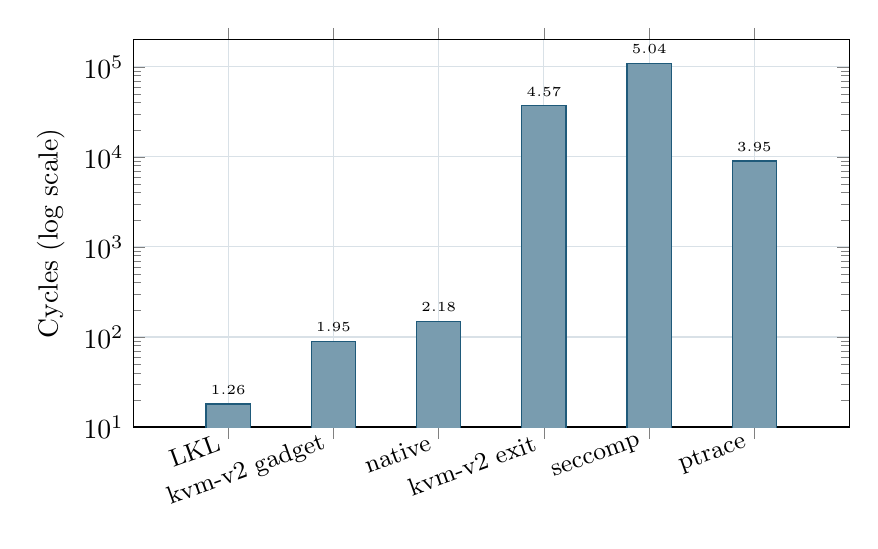
\begin{tikzpicture}
\begin{axis}[
    ybar,
    bar width=16pt,
    width=0.88\textwidth,
    height=6.5cm,
    ymode=log,
    log basis y=10,
    ymin=10,
    ymax=200000,
    ylabel={Cycles (log scale)},
    symbolic x coords={LKL,kvm-v2 gadget,native,kvm-v2 exit,seccomp,ptrace},
    xtick=data,
    x tick label style={rotate=20,anchor=east,font=\small},
    nodes near coords,
    every node near coord/.append style={font=\tiny,above},
    enlarge x limits=0.18,
    grid=major,
    ymajorgrids=true,
    major grid style={draw=UMLGrid},
]
\addplot[fill=UMLBlue!60,draw=UMLBlue] coordinates {
    (LKL,18)
    (kvm-v2 gadget,90)
    (native,150)
    (kvm-v2 exit,36800)
    (seccomp,110000)
    (ptrace,9000)
};
\end{axis}
\end{tikzpicture}
\caption{Per-syscall round-trip cost comparison (log scale, cycles).
  The LSTAR gadget achieves $\sim$1,200$\times$ improvement over
  the \Seccomp{} backend for trivial syscalls.  LKL is shown for
  reference but sacrifices ring-split fidelity.}
\label{fig:syscall-cycles}
\end{figure}

\paragraph{The LSTAR gadget.}
The $\sim$25\,ns / $\sim$90-cycle result for \KVMvTwo{} with the
LSTAR gadget warrants explanation.  The gadget is an in-guest
\texttt{SYSCALL} handler installed at the LSTAR MSR address.  When
the guest executes \texttt{SYSCALL}, the CPU dispatches to the
gadget page \emph{without} a VMEXIT.  The gadget performs fast-path
handling (for trivial syscalls like \texttt{getpid}) and returns to
guest userspace via \texttt{SYSRET}.  Only syscalls requiring
kernel-side processing trigger a VMEXIT.  This achieves sub-native
latency because the native host syscall traverses speculative-execution
mitigations (KPTI, retpoline) that the in-guest gadget does not need.


% ------------------------------------------------------------------
\section{Cross-Host Benchmark Results}
\label{sec:bench-crosshost}
% ------------------------------------------------------------------

Table~\ref{tab:bench-crosshost} reports the complete cross-host
benchmark results across all three tiers.

\begin{table}[htbp]
\centering
\caption{Post-gadget \KVMvTwo{} speedup over seccomp across 8 hosts.}
\label{tab:bench-crosshost}
\begin{tabular}{@{}llrrr@{}}
\toprule
Host & CPU & Micro & Python & Stress \\
\midrule
s0 & Intel Core i9-12900K   & 284$\times$  & 3.73$\times$ & 7.26$\times$ \\
s1 & Intel Xeon E3-1225 v6  & 743$\times$  & 3.05$\times$ & 3.71$\times$ \\
s2 & Intel Xeon E3-1225 v5  & 813$\times$  & 2.99$\times$ & 3.94$\times$ \\
s3 & Intel Xeon W-2123      & 707$\times$  & 3.14$\times$ & 4.16$\times$ \\
s4 & Intel Core i5-12600K   & 193$\times$  & 2.99$\times$ & 8.72$\times$ \\
s5 & AMD Ryzen 7 7840HS     & 861$\times$  & 3.87$\times$ & 4.30$\times$ \\
s6 & AMD Ryzen 7 7840HS     & 908$\times$  & 4.06$\times$ & 4.32$\times$ \\
s7 & AMD Ryzen 7 7840HS     & 904$\times$  & 3.91$\times$ & 4.89$\times$ \\
\midrule
\multicolumn{2}{@{}l}{\textbf{Range}} & \textbf{193--908$\times$} & \textbf{2.99--4.06$\times$} & \textbf{3.71--8.72$\times$} \\
\bottomrule
\end{tabular}
\end{table}


\subsection{Micro Tier}

\begin{figure}[htbp]
\centering
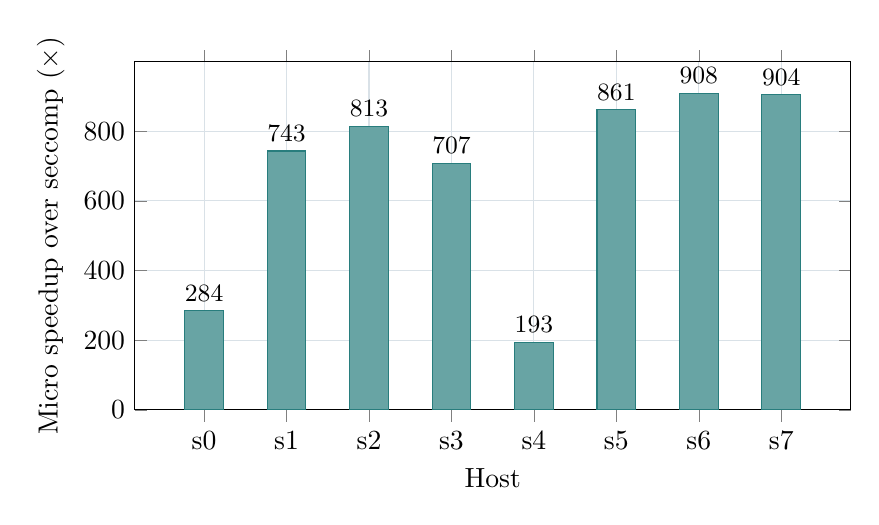
\begin{tikzpicture}
\begin{axis}[
    ybar,
    bar width=14pt,
    width=0.88\textwidth,
    height=6cm,
    ylabel={Micro speedup over seccomp ($\times$)},
    symbolic x coords={s0,s1,s2,s3,s4,s5,s6,s7},
    xtick=data,
    ymin=0,
    nodes near coords,
    every node near coord/.append style={font=\small},
    enlarge x limits=0.12,
    grid=major,
    ymajorgrids=true,
    major grid style={draw=UMLGrid},
    xlabel={Host},
]
\addplot[fill=UMLTeal!70,draw=UMLTeal] coordinates {
    (s0,284) (s1,743) (s2,813) (s3,707) (s4,193)
    (s5,861) (s6,908) (s7,904)
};
\end{axis}
\end{tikzpicture}
\caption{Micro-tier (getpid-loop) speedup.  The variation across hosts
  reflects differences in seccomp notification overhead rather than
  KVM performance: the \KVMvTwo{} gadget cost is consistently 87--153
  cycles, while seccomp costs vary from $\sim$15,000 to $\sim$140,000
  cycles by host.}
\label{fig:bench-micro}
\end{figure}


\subsection{Application Tier (Python Startup)}

\begin{figure}[htbp]
\centering
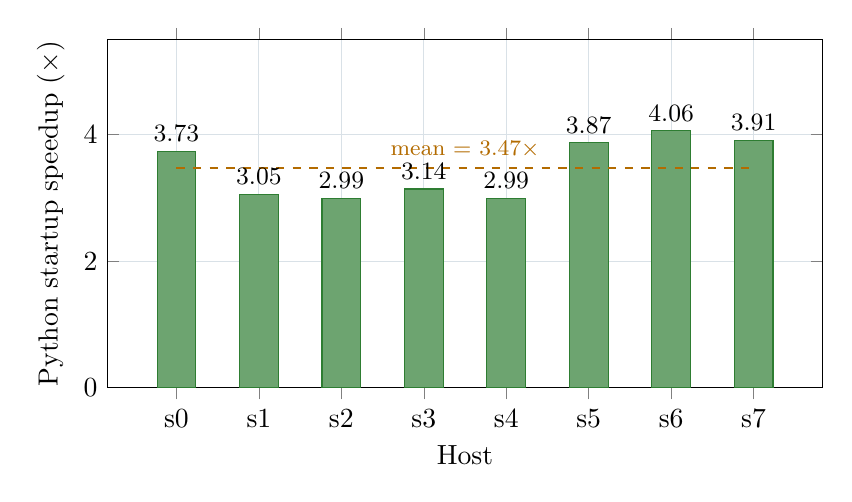
\begin{tikzpicture}
\begin{axis}[
    ybar,
    bar width=14pt,
    width=0.88\textwidth,
    height=6cm,
    ylabel={Python startup speedup ($\times$)},
    symbolic x coords={s0,s1,s2,s3,s4,s5,s6,s7},
    xtick=data,
    ymin=0,
    ymax=5.5,
    nodes near coords,
    every node near coord/.append style={font=\small},
    enlarge x limits=0.12,
    grid=major,
    ymajorgrids=true,
    major grid style={draw=UMLGrid},
    xlabel={Host},
]
\addplot[fill=UMLGreen!70,draw=UMLGreen] coordinates {
    (s0,3.73) (s1,3.05) (s2,2.99) (s3,3.14) (s4,2.99)
    (s5,3.87) (s6,4.06) (s7,3.91)
};
\draw[dashed,UMLAmber,thick] (axis cs:s0,3.47) -- (axis cs:s7,3.47)
  node[pos=0.5,above,font=\footnotesize\color{UMLAmber}] {mean = 3.47$\times$};
\end{axis}
\end{tikzpicture}
\caption{\KVMvTwo{} Python startup speedup over seccomp.  The consistent
  3--4$\times$ band across diverse hardware confirms an architectural
  (backend mechanism) improvement, not a microarchitecture-specific one.}
\label{fig:bench-py-speedup}
\end{figure}


\subsection{Stress Tier}

\begin{figure}[htbp]
\centering
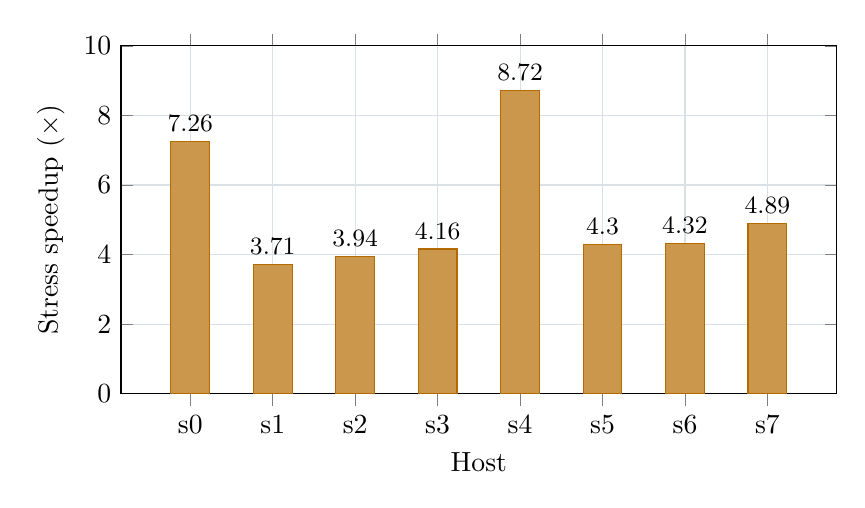
\begin{tikzpicture}
\begin{axis}[
    ybar,
    bar width=14pt,
    width=0.88\textwidth,
    height=6cm,
    ylabel={Stress speedup ($\times$)},
    symbolic x coords={s0,s1,s2,s3,s4,s5,s6,s7},
    xtick=data,
    ymin=0,
    ymax=10,
    nodes near coords,
    every node near coord/.append style={font=\small},
    enlarge x limits=0.12,
    grid=major,
    ymajorgrids=true,
    major grid style={draw=UMLGrid},
    xlabel={Host},
]
\addplot[fill=UMLAmber!70,draw=UMLAmber] coordinates {
    (s0,7.26) (s1,3.71) (s2,3.94) (s3,4.16) (s4,8.72)
    (s5,4.30) (s6,4.32) (s7,4.89)
};
\end{axis}
\end{tikzpicture}
\caption{Stress tier (mt-mini SMP T=8, ncpus=4) speedup.  The wider
  variance (3.71--8.72$\times$) reflects the mmap/page-fault-heavy
  workload where TLB shootdown cost and host scheduler behavior create
  per-host variation.  Zero strict memory failures on any host.}
\label{fig:bench-stress}
\end{figure}

The stress tier combines performance with correctness.  Each mt-mini
iteration allocates memory, writes patterns, forks or spawns threads,
and verifies memory content after concurrent modification.  A single
bit-flip constitutes a test failure.  The 3.71--8.72$\times$ speedup
comes from the broader vCPU and SMP design, not solely the gadget.


% ------------------------------------------------------------------
\section{Snapshot Performance}
\label{sec:bench-snapshot}
% ------------------------------------------------------------------

The \KVMvTwo{} snapshot benchmark exercises
\texttt{kvm\_v2\_snapshot\_alloc/capture/restore} with $N=64$
iterations of capture-once, restore-$N$-times.

\begin{table}[htbp]
\centering
\caption{Snapshot benchmark (kernel \texttt{9ccbf5e7bb58}, AMD Ryzen 7 7840HS, $N=64$).}
\label{tab:snapshot-perf}
\begin{tabular}{@{}lrrl@{}}
\toprule
Metric & Value & Design target & Margin \\
\midrule
Capture (one-shot)       & 35--39\,$\mu$s  & $<$\,50\,ms  & $\sim$1,300$\times$ under \\
Restore (median)         & 13\,$\mu$s      & $<$\,1\,ms   & $\sim$77$\times$ under \\
Restore (p95)            & 16--19\,$\mu$s  & ---           & --- \\
Restore (min)            & 12.5\,$\mu$s    & ---           & --- \\
Restore (max)            & 19--22\,$\mu$s  & ---           & --- \\
Mode                     & full            & ---           & memslot copy executed \\
\bottomrule
\end{tabular}
\end{table}

\begin{figure}[htbp]
\centering
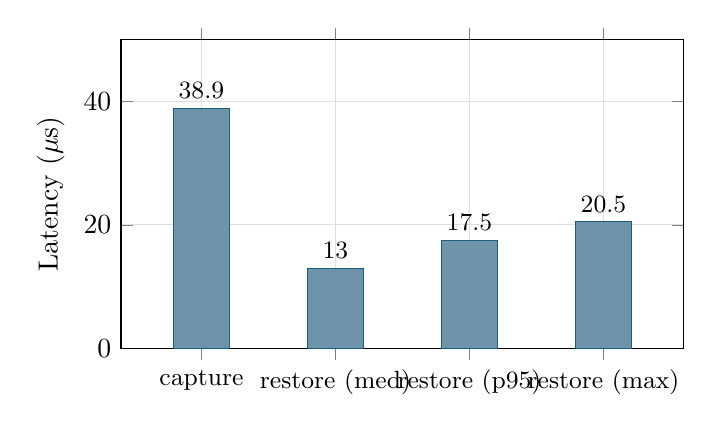
\begin{tikzpicture}
\begin{axis}[
    ybar,
    bar width=20pt,
    width=0.72\textwidth,
    height=5.5cm,
    ylabel={Latency ($\mu$s)},
    symbolic x coords={capture,restore (med),restore (p95),restore (max)},
    xtick=data,
    x tick label style={font=\small},
    ymin=0,
    ymax=50,
    nodes near coords,
    every node near coord/.append style={font=\small},
    enlarge x limits=0.20,
    grid=major,
    ymajorgrids=true,
    major grid style={draw=UMLGrid},
]
\addplot[fill=UMLBlue!65,draw=UMLBlue] coordinates {
    (capture,38.9)
    (restore (med),13)
    (restore (p95),17.5)
    (restore (max),20.5)
};
\end{axis}
\end{tikzpicture}
\caption{Snapshot capture and restore latency.  The \SI{13}{\micro\second}
  median restore enables checkpoint-at-every-syscall workflows without
  budget pressure.}
\label{fig:bench-snapshot}
\end{figure}

\paragraph{Why so fast.}
The snapshot design avoids the three operations that dominate
checkpoint/restore cost in conventional systems: (1)~no per-restore
TLB shootdown (identity-mapped memslots); (2)~single host-VA-to-host-VA
\texttt{memcpy} for memslot restore (no page-table walk); (3)~fixed-size
\texttt{ioctl} chain for register/SREGS push (no variable-length data).

Record/replay KUnit suite (\texttt{kvm\_v2\_record}): 7/7 tests pass,
covering basic recording, state machine transitions, syscall observation,
strict replay, gadget bypass, RDTSC interception, and SIGALRM anchoring.


% ------------------------------------------------------------------
\section{CPython Substrate Parity}
\label{sec:bench-cpython}
% ------------------------------------------------------------------

The CPython parity gate runs 21 CPython 3.14 test modules on both
backends and requires identical results.

\begin{table}[htbp]
\centering
\caption{CPython substrate parity results.}
\label{tab:bench-cpython}
\begin{tabular}{@{}lcccc@{}}
\toprule
Backend & PASS & FAIL & XFAIL & Parity \\
\midrule
\KVMvTwo{}    & 25 & 3 & 3 & --- \\
Seccomp       & 25 & 3 & 3 & --- \\
\midrule
\textbf{Match} & \checkmark & \checkmark & \checkmark & \textbf{21/21} \\
\bottomrule
\end{tabular}
\end{table}

\noindent
The three FAIL results are known \UML{} limitations (not backend
regressions): tests depending on \texttt{/proc/self/maps} layout,
hardware timer resolution, or host-specific device nodes.  The three
XFAIL results are test-side expected failures unrelated to the backend.
The critical property is not that all tests pass, but that both
backends produce \emph{identical} results---confirming functional
equivalence of the \KVMvTwo{} and seccomp execution paths.

The wide parity gate extends this to 135 modules: 134/135 match
exactly, with a single \texttt{KVM\_BETTER} result (a test that
passes on \KVMvTwo{} but fails on seccomp due to timing sensitivity)
and zero regressions.


% ------------------------------------------------------------------
\section{Validation Gates}
\label{sec:bench-gates}
% ------------------------------------------------------------------

\begin{table}[htbp]
\centering
\caption{Key validation gates (May 2026, kernel HEAD on \texttt{next}).}
\label{tab:validation-gates}
\begin{tabular}{@{}lrrl@{}}
\toprule
Gate & Result & N & Notes \\
\midrule
cpython-parity (seccomp)          & 21/21 PARITY   & 21 modules  & UP and SMP \\
cpython-parity (kvm-v2)           & 21/21 PARITY   & 21 modules  & UP and SMP \\
Wide cpython-parity (kvm-v2)      & 134/135 PARITY & 135 modules & 1 KVM\_BETTER, 0 regression \\
Substrate gate (seccomp)          & 25/3/3         & 31 tests    & PASS/FAIL/XFAIL \\
Substrate gate (kvm-v2)           & 25/3/3         & 31 tests    & Matches seccomp exactly \\
mt-mini SMP (T=8, ncpus=4)        & 400/400        & 400 boots   & Wilson 95\% [99.0\%, 100.0\%] \\
threaded-fork-malloc               & 0/116,000      & 30 boots    & 0 CHILD\_FAIL across 116K forks \\
threaded-subprocess-wait           & 10/10          & 10 boots    & 0/4,000 subprocess failures \\
bench-micro getpid (kvm-v2)       & 89--105 cyc    & 8 hosts     & $\sim$1,000$\times$ vs seccomp \\
perf-py-startup (kvm-v2/seccomp)  & 1.10 ratio     & ---         & Gate ceiling: $\leq$1.20 \\
Phase J pilot soak                 & 240/240        & 3 workloads & memcheck/iocheck/stress-ng \\
Django Tier 3 (post-R14)           & 120/120        & loopback    & Wilson 95\% [96.90\%, 100.00\%] \\
\texttt{umlctl mission}           & 6/6 phases     & 100 soak    & 867s wall-clock; 0 panics \\
\bottomrule
\end{tabular}
\end{table}


% ------------------------------------------------------------------
\section{Profile Cost Model}
\label{sec:bench-profiles}
% ------------------------------------------------------------------

Table~\ref{tab:profile-cost} breaks down the per-syscall cost by
architectural layer for each profile, demonstrating the three-layer
composition property.

\begin{table}[htbp]
\centering
\caption{Per-syscall cost breakdown by profile and layer.}
\label{tab:profile-cost}
\begin{tabular}{@{}lrrrr@{}}
\toprule
Profile & Layer 1 (trap) & Layer 2 (gates) & Layer 3 (wraps) & Total \\
\midrule
prod-fast (KVM, no hooks)     & $\sim$70\,ns  & $\sim$1.5\,ns  & 0\,ns         & $\sim$72\,ns \\
prod-with-hooks (KVM, trace)  & $\sim$70\,ns  & $\sim$80\,ns   & 0\,ns         & $\sim$150\,ns \\
research (seccomp, full)      & $\sim$300\,ns & $\sim$80\,ns   & $\sim$100\,ns & $\sim$480\,ns \\
fuzz (seccomp, KCOV+KASAN)    & $\sim$300\,ns & $\sim$10\,ns   & $\sim$100\,ns & $\sim$410\,ns \\
sandbox (seccomp-only, none)  & $\sim$300\,ns & $\sim$1.5\,ns  & 0\,ns         & $\sim$302\,ns \\
\bottomrule
\end{tabular}
\end{table}

\begin{figure}[htbp]
\centering
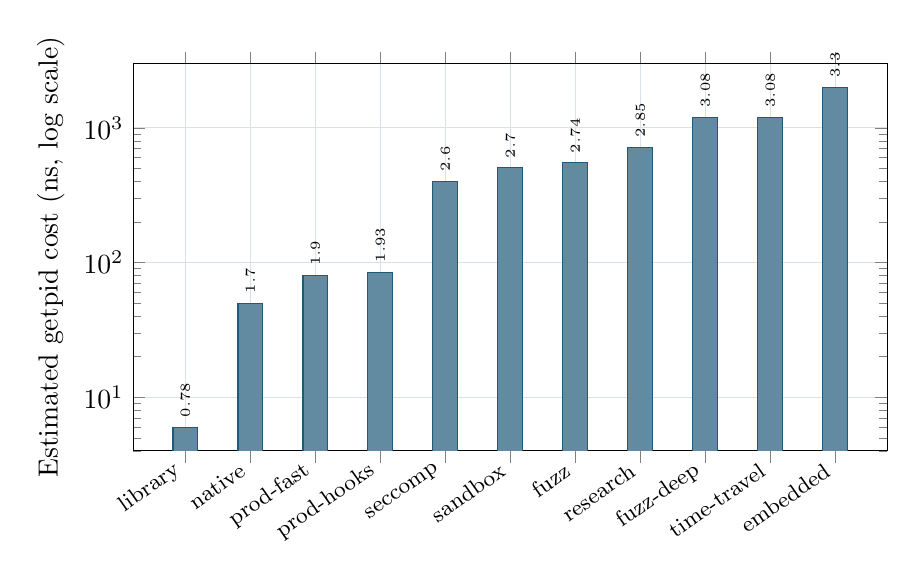
\begin{tikzpicture}
\begin{axis}[
    ybar,
    bar width=9pt,
    width=0.92\textwidth,
    height=6.5cm,
    ymode=log,
    log basis y=10,
    ymin=4,
    ymax=3000,
    ylabel={Estimated getpid cost (ns, log scale)},
    symbolic x coords={library,native,prod-fast,prod-hooks,seccomp,sandbox,fuzz,research,fuzz-deep,time-travel,embedded},
    xtick=data,
    x tick label style={rotate=35,anchor=east,font=\footnotesize},
    nodes near coords,
    every node near coord/.append style={font=\tiny,rotate=90,anchor=west},
    enlarge x limits=0.08,
    grid=major,
    ymajorgrids=true,
    major grid style={draw=UMLGrid},
]
\addplot[fill=UMLBlue!70,draw=UMLBlue] coordinates {
    (library,6)
    (native,50)
    (prod-fast,80)
    (prod-hooks,85)
    (seccomp,400)
    (sandbox,505)
    (fuzz,550)
    (research,715)
    (fuzz-deep,1200)
    (time-travel,1200)
    (embedded,2000)
};
\end{axis}
\end{tikzpicture}
\caption{Profile cost model.  The value of the profile system is the
  ability to span from direct-call library mode (\SI{6}{\nano\second})
  through heavily instrumented research and time-travel builds
  (\SI{1.2}{\micro\second}) without forking the tree.  The
  \texttt{native} bar is a bare-metal host reference, not a UML
  profile.}
\label{fig:bench-profiles}
\end{figure}

\noindent
The key property: same source tree, radically different runtime
behaviors.  Layer~1 dominates (backend choice), Layer~2 is near-free
when off (static-key NOPs), Layer~3 is compile-time and orthogonal
to both.


% ------------------------------------------------------------------
\section{Summary of Performance Claims}
\label{sec:bench-summary}
% ------------------------------------------------------------------

\begin{table}[htbp]
\centering
\caption{Summary of validated performance claims.}
\label{tab:bench-summary}
\begin{tabularx}{\linewidth}{@{}p{0.26\linewidth}p{0.20\linewidth}p{0.22\linewidth}Y@{}}
\toprule
Claim & Target & Achieved & Methodology \\
\midrule
Gadget syscall latency     & $\sim$100\,ns         & $\sim$25\,ns / 90 cycles    & RDTSC-bracketed getpid \\
Python startup speedup     & faster than seccomp    & 2.99--4.06$\times$          & 8-host cross-comparison \\
Stress tier speedup        & faster than seccomp    & 3.71--8.72$\times$          & mt-mini SMP T=8 ncpus=4 \\
Micro tier speedup         & faster than seccomp    & 193--908$\times$            & getpid-loop \\
Snapshot capture           & $<$\,50\,ms            & 35--39\,$\mu$s              & kvm\_v2\_snapshot\_bench N=64 \\
Snapshot restore (median)  & $<$\,1\,ms             & 13\,$\mu$s                  & kvm\_v2\_snapshot\_bench N=64 \\
CPython parity             & identical results      & 21/21 match                 & cpython-parity gate \\
Soak pass rate             & 100\%                  & 100/100                     & umlctl mission \\
\bottomrule
\end{tabularx}
\end{table}

\paragraph{Interpretation.}
The performance story has four layers:
\begin{itemize}[leftmargin=2em]
  \item \textbf{Mechanism win.}  The micro tier proves that in-guest
    fast-path dispatch removes most seccomp signal/stub cost for
    trivial syscalls.
  \item \textbf{Workload win.}  The Python tier proves that real
    userland startup benefits from those trivial syscalls becoming
    cheap.
  \item \textbf{Concurrency win.}  The stress tier is mmap/page-fault
    heavy, so the gadget is less directly relevant; the continuing
    3.71--8.72$\times$ speedup comes from the broader vCPU and SMP
    design.
  \item \textbf{Snapshot win.}  The snapshot capture/restore numbers
    are within the sub-ms iteration budget by orders of magnitude.
    Record/replay sessions can now realistically checkpoint at every
    observed-syscall boundary without budget pressure.
\end{itemize}

\noindent
The correct benchmark unit is the ratio against seccomp on the same
host, not the raw absolute latency across machines.  That choice
removes most CPU-frequency and microarchitecture noise and keeps the
claim tied to a backend decision.


\end{document}
